%更新：2015/01/25
\documentclass[a4j,12pt,makeidx]{jbook}
\usepackage{graphicx}
\usepackage{url}
\usepackage{makeidx}
\usepackage{here}
%しおり機能
\usepackage[dvipdfmx]{hyperref}
\usepackage{pxjahyper}
\usepackage{xcolor}
\hypersetup{
   bookmarksdepth=0,
   colorlinks=true,
   hyperfigures=frue
 }
 %
 %
\newcommand{\tp}{\thechapter}

\makeindex 
 \begin{document} 
 \title{Think Python：コンピュータサイエンティストのように考えてみよう\\
第二版}

 \author{アレン・B・ダウニー　\\
\\
\\
\\
相川利樹（日本語訳）}
 %\date{\today}
 \date{}
 \maketitle
 \vfill
 \begin{center}
（原題）Think Python: How to Think Like a Computer Scientist \\
2nd Edition \\
 （著者）Allen B. Downey
 \end{center}
 %%
 \vfill
 {\small
 Copyright\copyright 2018 相川利樹  \\
 「ThinkPython:コンピュータサイエンティストのように考えてみよう」（第二版） \\ by 相川利樹 is licensed under a Creative Commons 表示 3.0 非移植 License
 }
 \tableofcontents
 \clearpage
 \clearpage
 %
\phantomsection
 \addcontentsline{toc}{chapter}{はじめに}
 \chapter*{はじめに\markboth{はじめに}{}}
 \markboth{はじめに}{}
{\bf 本書の来歴} \par
１９９９年１月Javaを使ったプログラミング入門の講義の準備をしていた。これまで三回もこの講義を行っていたが、段々と嫌気が募ってきた。この講義の落第者の割合は高く、及第した学生の全体的な到達レベルもそんなに高くなかった。\par
　問題の一つは書籍だ。それらの書籍は余りにも大きく、必要以上にJavaの文法の細部にページを割き、如何にプログラムを組むかといった点に充分な組織的な配慮がなされてないものであった。それらの書籍の全てが「落とし穴」効果に犯されていた。つまり、最初は易しく、徐々に先に進むスタイルになっているが、第五章あたりから急に難しくなって床が抜けてしまう。学生たちは余りにも急に多くの新しいことにぶつかり、これ以降私は系統だった講義ができなくなり、切れ切れの講義をせざるをえないという状況に陥る訳だった。 \par
　講義開始の二週間前私は自分自身で本を書くことに決めた。目標は
\begin{itemize}
\item でき得る限り短く。同じ内容ならば五十ページを割くより、十ページで済ます方が学生の負担は少ない。
\item 語彙に注意する。呪文は最小限にし、語句は最初にキチンと定義して使う。
\item 徐々に組み立てる。「落とし穴」を避けるため、難しいテーマはそれを細分化したステップで構成する。
\item プログラム言語ではなく、プログラミングに焦点を当てる。最小限に必要なものだけでJavaを構成する。
\end{itemize}
本の題名は必要だった。そのとき心に浮かんだのが、「コンピュータサイエンティストのように考えてみよう」(``How to think like a computer scientist")である。　
私の第一版は荒削りなものであったが有効だった。学生たちはそれを読み、高度な話題や興味あるテーマにもクラスの時間を割けるほどの理解を示した。さらに、最も重要なことであるが、学生たちがそれらのテーマについての実習もできたことだ。私はこの本をGNU Free Documentation Licenseの下で出版した。このことはこの本のコピー、変更、さらに配布は利用者が自由にできることを意味していた。 \par
次ぎに起きたことは実にかっこいいことだった。バージニア州の高校教師、Jeff Elknerが私の本を引き継ぎ、それをPythonで書き直してくれた。そして、彼はその翻訳版を私に送ってくれた。私は私の書いた本を読んでPythonを学ぶという希有な経験をした。2001年にはGreen Tea PressからPython版の初版を出版した。 \par
2003年に私はOlin Collegeで教鞭を取り始め、そこで初めてPythonを教えることになった。やってみると、Javaのときと対照的に学生の躓きは少なく学習が進み、もっと興味有るテーマに取り組めるようになり、概して学生たちはより面白がった。\par
九年間以上かけて私は間違いを修正、サンプルプログラムを推敲、そして練習問題に多くの材料を追加し、この本を充実したものにしよう努力してきた。その結果誕生したのがこの本である。少し控え目に書名はThink Pythonとした。主な変更点を以下列記する。
\begin{itemize}
\item 各章の終わりにデバッギングに関する節を設けた。これらの節はバグを避けること、バグの発見の仕方の技術を扱っている。
\item 理解を助ける小テストからかなり本格的な課題までに渡り、多くの練習問題を追加した。そしてそれらの殆ど全てに解答を書いた。
\item 一連の事例研究を追加した。それらは課題、その解法、議論からなる少し長めの例題である。 
\item プログラム開発手法や基本的なデザインパターンの議論を拡張した。
\item デバッギング、アルゴリズムの解析に関する付録を追加した。
\end{itemize}
第二版では以下のような改訂を行った：
\begin{itemize}
\item 本の内容および関連するコードをPython3に即して更新した。
\item 初心者がPythonをインターネットブラウザで実行することができるように{\tt web}に関する新たな一節を追加した。
\item 第4.1節で導入した{\tt Swampy}と呼んだタートルグラフィックパッケージをPythonの標準のモジュールである{\tt turtle}に変更した。
\item 一つの新らしい章を追加した。この章は「便利グッズ」という題で必ずしも必要ではないがあれば便利だというPythonの特徴を導入した。
\end{itemize}
私はこの本を使うことで学習が楽しみになり、あなたの役に立ち少しでもコンピュータサイエンティストのように考えることができるようになることを期待する。\\
%\bigskip

\noindent
Allen B. Downey \\
Olin College
%
%
\chapter{プログラムが動くまで}
この本の目標は、如何にしたらコンピュータサイエンティストのように考えることができるかをあなたに教えることである。
そのような考え方は数学者、工学者、自然科学者のそれぞれの特徴を合わせ持っている。
数学者のように、コンピュータサイエンティストは自分のアイデアをコンピュータ上で実限させるために形式言語を使う。
工学者のように物ごとを設計し、部品を集めて一つのシステムを作り、さまざまの可能性の損得を評価する。
また、自然科学者のように、複雑系の振る舞いを調べ、仮説を立て、予測を検証する。\par
このコンピュータサイエンティストに求められる最も重要な能力は{\bf 問題解決能力（problem solving）}である。
問題解決能力は問題を定式化し、その解決について創造的に考え、その解決を明白にかつ正確に表現する能力のことである。
徐々に明らかになるが、プログラミングを学習するプロセスはこの問題解決能力を耕す大変に貴重な機会である。
この章を「プログラムが動くまで」とした理由もここにある。
一面では、プログラムの学習それ自体は有意義な能力開発である。
他面では、プログラミングは他の目的のための手段である。追々とその目的とは何かがはっきりしてくるはずだ。
\index{もんだいかいけつのうりょく@問題解決能力（problem solving）}
%
\section{プログラムとは何か}
一つの{\bf プログラム（program）}とは如何に計算を進めるのかということを特定した
一連の命令の集まりである。ここで計算といっているものは例えば方程式の解を求める、
多項式の根を求めるなどの数学的なものかもしれないが、
しかし、それは文書の中やプログラムの中（不思議に思えるが）のテキストを検索したり、置き換えをしたりすることでもある。\par
\index{プログラム（program）}
異なったプログラム言語で細部は異なってみえるが、基本的な命令はどのような言語でも確認できる： 
\begin{description}
\item [入力：] キーボード、ファイルそしてその他の様々な装置からデータを得る。
\item [出力：] 画面にデータを表示、ファイルやその他の装置にデータを書き出す。
\item [演算：] 加算や乗算のような基本的な数学的操作。
\item [条件実行：] 特定の条件を調べ、条件が満たされていると目的のコードを実行する。
\item [繰り返し：] ある動作を繰り返し実行する。大抵の場合何かを少しずつ変えて実行する。
\end{description}
信じられないことだが、これらはプログラムが持つべき機能の殆ど全てである。あなたが既に使ったどのプログラムも、
見かけは複雑にみえても、ここで述べた基本的な機能によく似た命令で出来上がっているのだ。
だからプログラミングとは全てを盛り込んだ大きなタスクをより小さい複数のタスクに分解し、
上記の基本的な機能の一つとして実行できるほど細かな多数のタスクに分解することである。\par
%
\section{Pythonを走らせる}
Pythonを勉強しようとして最初に挑戦しなければならないことの一つは
あなたのコンピュータにPythonや関連するソフトウエアをインストールすることかもしれない。
そのコンピュータのオペレーティング・システムに馴染んでいて、特にコマンドベースのインタフェース
に問題がなければPythonをインストールすることには何の問題もないであろう。しかし
初心者にとってシステム管理っぽいこととプログラミングを同時に学ぶことは苦痛になるかもしれない。\par
\index{ぱいそんをはしらせる@Pythonを走らせる（running Python）}
この問題を避けるために、インターネットブラウザ上でPythonを走らすことから始めることを推奨したい。
後にPythonに馴染んできた時点でPythonをインストールするための幾つかの示唆を提供することにしたい。\par
インターネットブラウザ上でPythonを動かす{\tt web}ページはいくつもある。あなたが好みの一つがあり
それを使っているならばそれを使うので構わない。さもなければ{\tt PythonAnywhere}を推奨したい。
これをから始めるための詳細を\url{http://tinyurl.com/thinkpython2e}で述べている。\par
\index{ぷらうだじょうでPython@ブラウザ上でPython（Python in a browser）}
\index{どこでもどこでもPython（PythonAnywhere）}
Pythonには二つのヴァージョンがある。これらはPython2とPython3と呼ばれている。二と大変に似ており
一つの学習すれば他のヴァージョンに移行することは極めて易しい。
この本はPython3について書かれた本であるが、必要に応じてPython2にも触れた。\par
\index{Pythonヴァージョン2（Python 2）}
Python{\bf インタプリタ（Interpreter）}はPythonで書かれたプログラム（Pythonコード）を読み実行するためのプログラムである。
環境によってアイコンをクリックしてこのインタプリタを起動することになるかコマンド入力で始めることになる。何れにしても
以下のような出力が表示されるはずだ：
\index{インタプリタ（interpreter）}
\begin{verbatim}
Python 3.4.0 (default, Jun 19 2015, 14:20:21) 
[GCC 4.8.2] on linux
Type "help", "copyright", "credits" or "license" ......
>>> 
\end{verbatim}
%
最初の三行はこのインタプリタやこれを走らせているオペレーティング・ｌｓシステムに関する情報である。だからあなたの画面に表示
されたものと若干異なるかもしれない。しかしPythonのヴァージョンナンバー（{\tt 3.4.0}）はこのインタプリタがPython3であることを
示すものであり、確認してほしい。それが{\tt 2}で始まっているとするとインタプリタはPython2である。\par
最後の行（山型の記号{\verb">>>"}） はインタプリタがユーザに入力可能状態を示す{\bf 入力請求記号（prompt）}である。
あなたがキーボードから{\tt 1+1}と入力しエンタキーを敲くとインタプリタは{\tt 2}と表示する。
\index{にゅうりょくせいきゅうもじ@入力請求記号（prompt）}
\begin{verbatim}
>>> 1 + 1
2
\end{verbatim}
これで出発の準備はできた。これ以降はPythonインタプリタを走らせコードを実行できる環境にあるとして話を進めることにしたい。
%
\section{初めてのプログラム}
\label{hello}
\index{Hello, World}
%
伝統的に新しい言語であなたが書く最初のプログラムは``Hello World!"と呼ばれるものである。
そのプログラムがすることの全ては画面に``Hello World"と表示することだからである。Pythonでは以下のようにある。
\begin{verbatim}
print( 'Hello World!')
\end{verbatim}
これが紙の上に何も印刷しないけれど、{\bf print文（print statement）}の一つの例である。
{\tt print}文は一つの値を画面に表示する。いまの場合それは単語で、
\begin{verbatim}
Hello World!
\end{verbatim}
である。プログラムでテキストの最初と最後を示す引用符号は結果には表示されない。
\index{いんよーふごう@引用符号（quotation mark）}
\index{ぷりんとぶん@print文（print statement）}
括弧はこの{\tt print}が関数であることを示す。第{\ref{funcchap}}章で関数は詳しく触れる。\par
\index{かんすう@関数（function）} 
\index{ぷりんとかんすう@print関数（print function）}
Python2では構文が少し異なり、それは関数ではないので括弧は使わない： 
\index{Pythonヴァージョン2（Python 2）}
\begin{verbatim}
print 'Hello World!'
\end{verbatim}
これらの区別は直ぐに意味のあるものであることがわかるが、今はこれで十分である。
%
\section{算術演算子}
\index{さんじゅつえんざんし@算術演算子（arithmetic operator）}
``Hello, World"の後は次のステップは計算である。Pythonはそのための{\bf 演算子（operators）}を提供している。
それらは加算や乗算の計算を表現するための特別な記号である。\par
演算子{\tt +}、{\tt -}そして{\tt *}は以下のように加算、減算、乗算を実行する：
\begin{verbatim}
>>> 40 + 2
42
>>> 43 - 1
42
>>> 6 * 7
42
\end{verbatim}
演算子{\tt /}は除算を実行する：
\begin{verbatim}
>>> 84 / 2
42.0
\end{verbatim}
何故結果が{\tt 42}でなく{\tt 42.0}なのか不思議に思うかもしれないが、次節で説明する。 \par
最後は演算子{\tt **}でべき乗算を実行する。ある数値をべき指数回乗算する：
\begin{verbatim}
>>> 6**2 + 6
42
\end{verbatim}
ある種のコンピュータ言語では記号{\verb"^"}がべき乗算に使われることがあるが、Python
ではこの記号は{\tt XOR}と言われるビット演算子である。
このビット演算子に馴染みがないとする、以下の結果に驚くかもしれない：
\begin{verbatim}
>>> 6 ^ 2
4
\end{verbatim}
この本ではビット演算については触れない。興味のある人は \url{http://wiki.python.org/moin/BitwiseOperators}.
を読んでほしい。
\index{びっとえんざんし@ビット演算子（bitwise operator）}
%
\section{値と型}
\index{value}
\index{type}
\index{string}
{\bf 値（value）}は文字や数値のようなプログラムに関わる基本的なものである。
これまでに出会った値は{\tt 2}、{\tt 42.0}それに{\tt 'Hello World!}'である。\par
これらの値は異なった{\bf 型（types）}に属している。
つまり{\tt 2}は{\bf 整数（integer）}であり、{\tt 42.0}は{\bf 浮動小数点数（floating point）}であり、
{\tt 'Hello world!'}は文字の列を含んでいるので、{\bf 文字列（string）}である。\par
\index{integer}
\index{floating-point}
ある値がどの型であるか不明なときはインタプリタが教えてくれる：
\begin{verbatim}
>>> type(2)
<class 'int'>
>>> type(42.0)
<class 'float'>
>>> type('Hello, World!')
<class 'str'>
\end{verbatim}
%
これらの結果では``class"という単語は部類（カテゴリー）の意味で使われている。
\index{class}
つまり一つの型は値が属する一つの類概念のことである。
当然だが、整数は{\tt int}型に、文字列は{\tt str}型に属し、小数点を含む数値は{\tt float}型に属する。\par
\index{type}
\index{string type}
\index{int type}
\index{float type}
ところで、{\tt '2'}や{\tt '42.0'}は何型かな？　数値のようにみえるが、文字列のように引用符で括られている。
\begin{verbatim}
>>> type('2')
<class 'str'>
>>> type('42.0')
<class 'str'>
\end{verbatim}
%
これらは{\tt str}型に属する、つまり、文字列である。\par
\index{quotation mark}
大きな数を表示するとき、{\tt 1,000,000}の様に三つの数字毎にカンマを入れることがある。これはPythonの世界では不正な整数であるが、合法的だ。
\begin{verbatim}
>>> 1,000,000
(1, 0, 0)
\end{verbatim}
まあ、期待したものではないが。Pythonインタプリタはカンマで区切られた三つの整数の配列だと解釈する。このような配列の関しては後にさらに
学習するはずだ。
\index{はいれつ@配列（sequence）}
%
\section{形式言語と自然言語}
{\bf 自然言語（natural language）}は英語、スペイン語、フランス語のように人々が話している言語である。
それらは（人々はこれらに対してある規範を課そうとするが）人工的に設計されたものではない。これらは自然と進化したのだ。\par
{\bf 形式言語（formal language）}はある特別の用途のために人工的に設計された言語である。
例えば、数学で用いる記号は数や記号の間の関係を記述する上で適切な形式言語である。
化学者は分子の化学構造を示すために形式言語を用いる。そして、さらに重要なことであるが、\par
\bigskip
{\bf プログラム言語は計算を表現するために設計されてきた形式言語である。} \par
\bigskip
形式言語はその構文が厳格になる傾向がある。例えば、{$3+3=6$}は数学的には正しい構文で作られた文である。
しかし、{$3 + = 3$ \mbox{\$} $6$}はそうでない。
 {$H_2O$}は化学的には正しい構文で作られた文である。 {$_2Zz$}はそうでない。\par
構文のルールは二つ特徴物からなる、つまり{\bf 字句（tokens）}と{\bf 文法（sturucture）}である。
字句は単語、数、化学元素のような言語の基本要素である。{$3 + = 3$ \mbox{\$} $6$}が不正である一つの理由は\mbox{\$}が数学的に正しい字句でないことである。また、 {$_2Zz$}では省略形 で表現される元素がないことである。\par
構文エラーの二つ目は文の文法に関連するものだ。つまり、字句の並べ方のよるものだ。{$3+=3$}という文は{$+$}や{$=$}は正しい字句であるが、
隣接して使うことは不正である。同じように、化学式では元素記号の後に添え字が付き前ではない。\par
英文を例に取ると：
\begin{quote}
This is @ well-structured Engli\$h
sentence with invalid t*kens in it.  This sentence all valid tokens
has, but invalid structure with.
\end{quote}
ここで最初の文は不正な字句を含む文法的に正しい英文の例であり、二番目は有効な字句からなる文法的に不正な英文の例である。\par
あなたが英文や形式言語の文を読んでいるとき、
あなたはその文の構文がどうなっているか確認しなければならない（自然言語のばあいはこれを無意識に行っている）。
このような過程を{\bf 構文解析（parsing）}と言う。\par
形式言語と自然言語は多くの共通点、字句、文法、構文、意味があるが、いくつかの違いがある：
\begin{description}
\item [曖昧さ（ambiguity）：] 自然言語は曖昧さに満ちあふれている。
人々は文の中味に手懸かりを求め、他の情報を使ってこの曖昧さに対処している。
形式言語は、文の中味に拘わらず、ほぼまたは完全に曖昧さを排除するように設計されている。
\item [冗長性（redundancy）：] 自然言語では曖昧さがあることや誤解を避けるために、冗長性を高めている。
その結果、自然言語はだらだらしたものになる。形式言語は冗長性を減らしその結果簡明なものになっている。
\item [逐語性（literalness）：] 自然言語は慣用句や比喩に満ちあふれている。
わたしは``The penny dropped"と言ったとしても、もしかするとそこには``penny"も``dropping"もないかもしれない
（この慣用句的な表現は“目から鱗が落ちる”という意味だ）。一方、形式言語ではそこで言われたことがそのままの意味になる。
\end{description}
自然言語を喋って育った人々は形式言語に慣れることに多々苦労する。ある意味では、この相違は詩と散文の違いに似ているが、それ以上だ：
\begin{description}
\item [詩（poetry）：] 単語はその意味と同時に音韻のためにも使われる。
詩全体によって感情の起伏を作り出す。曖昧さの高さは一般的ばかりでなく、意図的だ。
\item [散文（prose）：] 単語の逐語的な意味はもっと重要になり、文法はより意味を持つようになる。
散文はより素直に解析できるが、多くのばあい曖昧さは多い。
\item [プログラム（program）：] 一つのコンピュータプログラムが持っている意味は唯一で曖昧さがなく、字句と文法の解析で完全に理解できる。
\end{description}
ここでプログラム（その他の形式言語でも）を読む上で留意すべき点を列記する。
第一に形式言語は自然言語に比較して稠密なことだ。そのためそれを読むためには時間を要する。
また、文法は極めて重要だ。従って、上から下、右から下へと読み下すことは薦められない。
そのかわり、字句を特定し、文法的な解釈を頭でしながら、構文解析をすべきだ。最後に、細かなことであるが、
自然言語では見過ごしてもよいような綴りや句読点の僅かな間違いが形式言語では重大な相異を生み出す。
%
\section{デバッギング}
プログラミングにはエラーは付き物だ。いたずら心から、プログラミングに起因するエラーは{\bf バグ（bugs）}と呼ばれる。そしてこのバグ取りの過程を{\bf デバッギング（debugging）}と呼ぶ。\par
プログラミングや特にデバッギングはときとして心理的な葛藤を呼び起こすことがある。もしあなたが困難なバグに格闘しているとすると、怒り、失望、恥ずかしさの感情を持つかもしれない。\par
　人々がこのような状況におかれるとコンピュータがあたかもヒトであるように対応することはよく知られていることである。作業が上手くいっていると我々はコンピュータを僚友と感ずる、そして、コンピュータが意地悪で、言うことを聞いてくれないと、我々はそのようにヒトに対して振る舞うように、コンピュータに対しても振る舞う（Reeves and Nass, ``The Media Equation: How People Treat Computers, Television, and New Media Like Real People and Plays"）。
このようなヒトの反応に対して心構えをしておくことは賢明だ。一つの接近法はコンピュータを例えば、速度や精度に対して特殊な能力を持っているが、物事を斟酌し、大枠を捉えることに極端に弱点のある従業員と考えることである。\par
あなたの仕事は優秀なマネージャであることである。つまり、その長所を活かし、弱点を補強する方法を探すことだ。そして、コンピュータに対するあなたの感情が仕事をする上で邪魔にならないよう、あなたの感情を問題解決することに集中する方法を探すとよい。\par
デバッグの方法を学ぶことは期待したものではないかもしれない。しかし、これはプログラミングという枠を超えて多くに仕事にも役にたつものである。各章の終わりにここで述べたようなデバッグの節を設けた。あなたの助けになればなによりだ。
%
\section{語句}
\begin{description}

\item[問題解決能力（problem solving）：]問題を定式化し、解を見つけそしてそれを表現する過程。
%\index{problem solving}

\item[高級言語（high-level Language）：]Pythonのような、人にとって読み書きが容易になるように設計されたプログラム言語。
%\index{high-level language}

\item[低級言語（low-level Language）：]コンピュータにとって実行が容易であるよに設計されたプログラム言語。「機械語」とか「アセンブリ言語」と呼ばれる。
%\index{low-level language}

\item[移植性（portability）：]一種以上のコンピュータ上で実行可能な性質。
%\index{portability}

\item[入力請求記号（prompt）：] インタプリタでユーザからの入力を受けることが可能になっていることを示すための文字列。
%\index{prompt}

\item[プログラム（program）：] 一連の計算を実行するための一連の命令の集まり。.
%\index{program}

\item[print文（print statement）：]Pythonインタプリタが画面上に値を出力することを意図した命令。 
%\index{print statement}
%\index{statement!print}

\item[演算子（operators）：]加法、乗法そして文字列の連結などの単純な計算を表現する特な記号。
%\index{operator}

\item[値（value）：]プログラムが操作する数値や文字列のような基本的データの実体。
%\index{value}

\item[型（types）：] 値が持つ属性。これまで出会ったのは整数（{\tt int}型）、浮動小数点数（{\tt float}型）そして文字列({\tt str}型）である。
%\index{type}

\item[整数（integer）：]全ての数を表現する型。
%\index{integer}

\item[浮動小数点数（floating point）：]小数点以下を持つ数値を表現する型。
%\index{floating-point}

\item[文字列（string）：]文字の列を表現する型。
%\index{string}

\item[自然言語（natural language）：]人類の進化と共に進化したヒトが話す言語。
%\index{natural language}

\item[形式言語（formal language）：]数学的な考えやコンピュータのためのプログラムのように特別な目的のために設計された言語。
そして全てのプログラミング言語は形式言語である。
\index{formal language}

\item[字句（tokens）：]自然言語の単語に類似したプログラムの意味的構造上の基本要素の一つ。
%\index{token}

\item[構文（syntax）：]プログラムの構造。
%\index{syntax}

\item[構文解析（parsing）：]形式文法に従ってプログラムを解析すること。  
%\index{parseing}

\item[バグ（bugs）：] プログラムに潜んでいるエラー。
%\index{bug}

\item[デバッギング（debugging）：]プログラムに潜む三種類のエラーを見つけ取り除く作業。 
%\index{debugging}

\end{description}
%
\section{練習問題}
\noindent
{\bf 練習問題\tp.1} この本を読むときには、あなた自身で例題がどう動くか確認しつつ進めるようコンピュータを前にして読んでほしい。\par
新しいテーマに出会うたびに、間違いをすべきである。例えば、``Hello World!"プログラムである。
{\tt print}文で使っている引用符（{\tt '}）の一つがないと何が起きるか？二つないと何が起きるか？{\tt print}の綴りを間違えると何がおきるか？\par
このような間違いを犯した経験は、このような間違いをするとそのとき表示されるエラーメッセージの意味を確認できるので、
この本で読んだことが何であったかの記憶を助けてくれ、デバッギングの助けにもなる。
早い内に、それも意図的に間違いをしてみる方は後に偶然にそれをするより賢明だ。\par
\begin{enumerate}
\item {\tt print}文でカッコの一つまたは双方を外すと何がおきるか？
\item 文字列の引用符の一つまたは双方を外すと何がおきるか？
\item -2のような負の数を表現するのにマイナス符号{\tt -}を付ける。もしある数の前に{\tt +}の符号を付けると何がおきるか？また{\tt 2++2}では
何がおきるか？
\item 数学では02のように数字の前にゼロを書くことは許されている。Pythonでは何がおきるか？
\item 演算子なしで二つの数字を並べて書くと何がおきるか？
\end{enumerate}

\noindent
{\bf 練習問題\tp.2} Pythonインタプリタを起動し、計算をしてみよう。
\begin{enumerate}
\item 42分42秒は何秒か？
\item 10キロメートルは何マイルか？（ヒント：1マイルは1.61kmである。）
\item 10キロメートル競技を42分42秒で完走した。１マイルあたり掛かった平均時間（分と秒を使って）はいくらか？
また、マイル毎時で表現した速度はいくらか？
\end{enumerate}
%
\chapter{変数、表式、文}
プログラム言語の強力な機能の一つは{\bf 変数（variable）}が扱えることだ。変数は値を参
照するための付けられた名前である。\par
%
\section{代入文}
{\bf 代入文（assignment statement）}によって変数は生成され、それに値が与えられる：
\begin{verbatim}
>>> message='And now for something completely different'
>>> a=17
>>> pi=3.141592653597932
\end{verbatim}
これらの例では三つの代入文を生成した。
最初の例では文字列の代入を新しい変数{\tt message}に、
二番目では整数17の代入を変数{\tt a}に、最後の例では、円周率$\pi$ の近似値を変数{\tt pi}に代入した。
紙の上で変数を表現するために良く用いられる方法は新しい名前を書きその変数が持つ値に向けて矢印を書くというものだ。
この種の図は各変数の現在の状態（心の変動状態のように考えて）{\bf 状態図（state diagram）}と呼ぶ。図\ref{fig.state2}は前の例の状態図である。 
%
\begin{figure}[htbp]
\centerline
{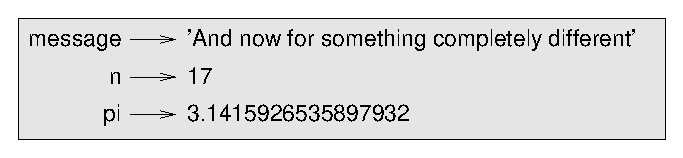
\includegraphics[scale=0.8]{figs/state2.eps}}
\caption{状態図}\label{fig.state2}
\end{figure}　
%
\section{変数名}
プログラマーは一般的にそれが何のために用いられているかが分かるように意味がある変数名を選ぶ。\par
変数名はいくらでも長くできる。それらは文字と数字を含んでいても構わないが、先頭は文字でなければならない。
大文字も合法的だが、先頭文字は小文字にするのが賢明だ（理由は後で分かる）。\par
アンダースコア文字、{'\_'}も名前に付けてよい。これは例えば、\\
{\tt my\_name}や{\tt airspeed\_of\_unladen\_swallow}のように、単語を結びつけて使うときに頻繁に使う。\par
あなたが不正な名前を使うと構文エラーになる：
\begin{verbatim}
>>> 76trombones = 'big parade'
SyntaxError: invalid syntax
>>> more@ = 1000000
SyntaxError: invalid syntax
>>> class = 'Advanced Theoretical Zymurgy'
SyntaxError: invalid syntax
\end{verbatim}
{\tt 76trombones}は先頭が文字で始まらないので不正な名前である。{\tt more@}は不正な文字を含むので不正である。では、{\tt class}は？
実は、{\tt class}はPythonの{\bf 予約語（keywords）}である。
インタプリタはプログラムの構造を認識するためにこれらの予約語を使い、変数名として使うことができない。\par
Python3は以下のような予約語がある：
\begin{verbatim}
False      class      finally    is         return
None       continue   for        lambda     try
True       def        from       nonlocal   while
and        del        global     not        with
as         elif       if         or         yield
assert     else       import     pass
break      except     in         raise
\end{verbatim}
これらを記憶しておく必要はない。大抵の開発環境ではこれらの予約語は異なった色で表示されるので、
それを間違って変数として使ったとしても直ぐ分る。
%
\section{表式と文}
一つの{\bf 表式（expression）}は値、変数、演算子の組み合わさったものである。
一つの値のみも表式であり、変数一つもそうである。従って以下の表式は合法的である：
\begin{verbatim}
>>> 42
42
>>> n
17
>>> n + 25
42
\end{verbatim}
入力請求記号（{\tt >>>}）に続き表式が入力されると、インタプリタはそれを{\bf 評価（evaluates）},つまり表式の値を求める。
この例では{\tt n}は値17を持ち、{\tt n+25}は値42を持つ。\par
一つの{\bf 文（statement）}は変数を生成するまたは値を表示するといったPythonインタプリタが実行できるソースコードの単位である。
\begin{verbatim}
>>> n = 17
>>> print(n)
\end{verbatim}
一行目は{\tt n}の値を与える代入文であり、二行目は変数{\tt n}が持つ値を表示する{\tt print}文である。\par
文を入力するとインタプリタはそれを{\bf 評価（evaluates）},つまり文が意味することは何かを探る。一般に文は値を持たない。
%
\section{スクリプト・モード}
これまではわれわれはPythonをインタプリタは{\bf インタラクティブ・モード（interactive mode）}で使ってきた。
このモードではあなたがキーボードからプログラムを入力するとインタプリタは即結果を画面に表示した。このモードは
習い始めにはよい方法だが数行に渡るコードを書こうとすると、このモードは足手まといになる。\par
別な方法はコードを{\bf スクリプト（script）}と呼ばれるファイルに保存し、その後このスクリプトを実行するためにPythonを
{\bf スクリプト・モード（script mode）}で走らせる方法である。Pythonスクリプトは慣例に従って{\tt .py}の拡張子を使う。\par
スクリプトの生成やコンピュータ上で如何にスクリプトを実行するかといったことが了解済みならば先に進めるはずだ。
さもなければPythonAnywhereを再度使うことをお薦めしたい。スクリプト・モードでのPythonの実行方法は
別途に\url{http://tinyurl.com/thinkpython2e}に纏めておいた。\par
.Pythonは二つのモードを提供しているので、ソースコードをスクリプトとしてまとめて書く前に、そのコードを少しずつテストできる。
しかし、インタラクティブ・モードとスクリプト・モードの間には若干の相異があり、混乱を引き起こすかもしれない。\par
例えば、以下はPythonを電卓のように使う例である：
\begin{verbatim}
>>> miles = 26.2
>>> miles * 1.61
42.182
\end{verbatim}
一行目は変数{\tt miles}への代入文であり、結果はなにも表示されない。
二行目は表式で、インタプリタはこの表式を評価し、その結果を表示する。
これでマラソン競技は約42kmの距離を走ることが分かる。\par
しかし、この二行をそっくりスクリプトとして書き、実行しても何も表示されない。
スクリプト・モードでは表式それ自体には表示機能がない。
スクリプト・モードでも表式は評価されるが、表示は別だということである。スクリプトでは以下のように書く：
\begin{verbatim}
miles = 26.2
print miles * 1.61
\end{verbatim}
最初はこのことで混乱するかもしれない。\par
スクリプトは通常複数の文を含む。複数の文があるときは、結果はそれらの文が一度に一つずつ実行される。\par
スクリプトの例を示す：
\begin{verbatim}
print(1)
x = 2
print(x)
\end{verbatim}
これを実行した結果の表示は
\begin{verbatim}
1
2
\end{verbatim}
となる。代入文には表示するものがない。\\
理解を確認するために、以下のような表現をPythonインタプリタで入力し、何が表示されるか調べよてみよう：
\begin{verbatim}
5
x = 5
x + 1
\end{verbatim}
さて、同じ表現をスクリプトとして書き、そのスクリプトを実行してみよう。
スクリプトを修正して、各表式を{\tt print}文のカッコの中に入れて実行してみよう。
%
\section{演算子の順位}
表式に一つ以上の演算子が含まれていると、その表式の評価は{\bf 優先順位（rule of precedence）}による。数学的な演算子については、Pythonは数学的慣用に従う。{\bf PEMDAS}という頭字語として覚えるとよい。
\begin{itemize}
\item 括弧は最も高い優先度を持つ、そしてこれによってある表式の評価をあなたが必要とする順位で処理させることができる。
括弧で括られた表式が最初に評価されるので{\tt 2 * (3-1)}は{\tt 4}であり、{\tt (1+1)**(5-2)}は{\tt 8}である。
また、あなたは括弧を表現の見やすさのために用いることもできる。{\tt (minute * 100) / 60}では括弧はなくても結果は同じになる。
\item べき乗算は次ぎに高い順位を持つ演算子である。だから、{\tt 2**1+1}は{\tt 3}であり、{\tt 4}ではない。また、{\tt 3*1**3}は{\tt 3}であり、{\tt 27}ではない。
\item 乗算、除算は加算、減算（この二つも同じ優先度である）より優先度が高く、同じ優先度を持つ。
だから、{\tt 2*3-1}は{\tt 5}であり、{\tt 4}ではない。同じく、{\tt 6+4/2}は{\tt 8}であり、{\tt 5}ではない。
\item 同じ優先度を持つ演算子は左から右へ（例外はべき乗算）と評価される。だから、表式{\tt degree /2 * pi}は除算が最初で、その結果に{\tt pi}がかけられる。$2\pi$で割ることを意図したのであれば、括弧を使うか、{\tt degree/2/pi}とする。
\end{itemize}
わたしは他の演算子についての優先順位を憶えることにあまり熱心でない。表式がそれらしくみえないときは、括弧を使い明確にすることにしている。
%
\section{文字列処理}
一般に算術的な演算をそれが見かけの上で数のようであっても文字列に施すことはできない。従って、以下のような演算は不正である：
\begin{verbatim}
'2'-'1'     'eggs'/'easy'	     'third'*'a charm'
\end{verbatim}
演算子{\tt +}は文字列に作用できるが、あなたが期待したものではないかもしれない。これは文字列の{\bf 連結（concatenation）}、つまり、
文字列と文字列の端と端を結合することである。例を挙げると
\begin{verbatim}
>>> first = 'throat'
>>> second = 'warbler'
>>> first + second
throatwarbler
\end{verbatim}
表示されるものは{\tt throatwarbler}である。\par
演算子{\tt *}も文字列に使え、文字列の繰り返しを行う。例として、{\tt 'Spam' * 3}は{\tt SpamSpamSpam}の表示を得る。被演算子の一つが文字列ならば、他は整数というかたちでなければならない。
これらの演算子{\tt +、*}の使用法は算術演算子として持つ機能を考えれば納得がゆくものであろう。{\tt 4*3が4+4+4}と同値であるように、{\tt 'Spam' * 3}は{\tt 'Spam'+'Spam'+'Spam'であろうからである。\par
一方、この文字列の連結処理や繰り返し処理と整数の加算、乗算とは異なるところがある。
文字の連結ではできないが整数の加算ではできる性質の一つを思い浮かべることができるか？
%
\section{コメント}
プログラムが大きくなり、より複雑になるとプログラムを読むことが難しくなる。
形式言語は稠密なので、コードの一部分を眺めてそこで行われていることを理解することが多々困難なことがある。\par
そこでプログラムの中に自然言語でそこで行われていることについての注釈を追加することは賢明である。
これらは{\bf コメント（comments）}と言われ、記号{\tt \#}で始まる：
\begin{verbatim}
#compute the percentage of the hour that are elapsed
percentage = (minute * 100) / 60
\end{verbatim}
この例ではコメントは一行に書いた。行の終わりに置くこともできる：
\begin{verbatim}
percentage = (minute * 100) / 60 # percentage of an hour
\end{verbatim}
記号{\tt \#}から行の終わりまでがコメントで、プログラムには何の影響も持たない。\par
コメントはそのコードの部分に自明でない特徴がある場合に有効である。
コードを直接眺めることでそこで何が行われているかが分かる方が説明を追加するより好ましいことには論を待たない。\par
以下のコメントは冗長で無意味である：
\begin{verbatim}
v = 5  #assign 5 to v
\end{verbatim}
以下のコメントはコードのみでは得られない情報を含むので有用だ：
\begin{verbatim}
v = 5  #velocity in meters/second.
\end{verbatim}

変数の付け方が上手いとコメントの量を少なくできるが、長い名前は表式を複雑にさせ読み辛いものになるので、損得を天秤かける必要がある。
%
\section{デバッギング}
プログラムでは三種類のエラーが起こりうる。つまり、構文エラー、実行時エラー、意味的エラーである。これらの三種類のエラーを区別し、バグ取りが効果的に行えるようにするとよい。
\begin{description}
\item[構文エラー：] {\bf 構文（syntax）}とはプログラムの構造に言及したもので、その構造が持つべきルールである。
例えば、カッコは右左を揃えて使わなければならない、だから{\tt (1+2)}は合法であるが、{\tt 8)}は{\bf 構文エラー（syntax error）}になる。　\par
あなたのプログラムが構文エラーを一つでも含んでいると、Pythonはそのエラーに対してエラーメッセージを出し、
そこでプログラムの実行を停止する。プログラミングの経験の浅い初めの数週間はこの種の構文エラーのバグ取りにかなりの時間を費やすだろう。
しかし、経験を積むに従ってエラーをする度合いは減るし、エラーを容易く発見できるようになる。
\item[実行時エラー：] 第二のエラーはプログラムが実行されるまでは現れないので実行時エラーと呼ばれているものである。
これらのエラーはプログラムを実行しているときに何か例外的（そして悪い）な状況が起きたときに出るエラーなので{\bf 例外（exceptions）}とも呼ばれている。\par
簡単なプログラムでは実行時エラーは希であるので、それに遭遇するまでは暫くかかる。
\item [意味的エラー：] 第三のエラーは{\bf 意味的エラー（semantic error）}である。
意味的エラーがあってもコンピュータはエラーメッセージを出さないでプログラムは成功裡に実行さたようにみえる。しかし、結果が間違っている。意図したことと別なことが実行された訳である。特に、間違っているにせよ、あなたがせよと命じたことが行われているからだ。\par
問題は書き上げたプログラムがあなたが書こうとしたプログラムでないことである。プログラムの内容（従ってその意味）が間違っている訳である。この意味的なエラーを探し出すことはきわどい仕事である。なぜならば、コンピュータの出力結果をみてソースプログラムの間違いを探り当てるという後ろ向きの作業をしなければならないからだ。　
\end{description}
%
\section{語句}
\begin{description}
\item[変数（variable）：]一つの値を参照するための名前。
%\index{variable}

\item[代入文（assignment statement）：]一つの値を一つの変数に割り当てる文。
%\index{assignment}

\item[状態図（state diagram）：]値の一組とそれらを参照する変数の一組の関係を示すグラフィックな表現。.
%\index{state diagram}

\item[予約語（keywords）：]コンパイラがプログラムを構文解析するために予め使うことを予定してある単語。あなたの
プログラムでは{\tt if}、{\tt  def}そして {\tt while}のような単語を変数名として使うことができない。.
%\index{keyword}

\item[被演算子（operands）：]演算子が作用する値。 
%\index{operand}

\item[表式（expression）：]変数、演算子そして値を組み合わせて一つの計算を表現した式。結果は一つの値になる。 .
%\index{expression}

\item[評価（evaluate）：] 一つの単独な値を生成するために演算を実行して表式を簡潔にする。
%\index{evaluate}

\item[文（statement）：]一つの命令や動作を表現するコードの一段落。 これまでに出会ったのは代入文そしてprint文である。
%\index{statement}

\item[実行（execute）：] 一つ文を実行しすることそしてその文が意味することを行う。
%\index{execute}

\item[インタラクティブ・モード（interactive mode）：] 入力請求時にコマンドや表式を入力することによってPythonインタプリタを使う方式。
%\index{interactive mode}

\item[スクリプト・モード（script mode）：] 一つのスクリプトを読み込みそれを一気に実行するようなPythonインタプリタの使い方。
%\index{script mode}

\item[スクリプト（script）：]一つのファイルとして保存されたプログラム（通常はインタプリタで実行される）。
%\index{script}

\item[優先順位（rule of precedence）：]複数の演算子とを含む表式の評価（結果の値を出す）する際に適用される演算の順序に関する規則。
%\index{rules of precedence}
%\index{precedence}

\item[連結（concatenation）：]二つの被演算子を端と端で繋ぐこと。 
%\index{concatenation}

\item[コメント（comments）：]他のプログラマー（またはそのソースコードを読む）人たちのためにプログラムに書き込む情報。プログラムの実行には何の効果も無い。  
%\index{comment}

\item[構文エラー（syntax error）：]構文解析が不可能になるようなプログラム上のエラー（そしてそれ故インタプリタもエラーを出す）。
%\index{syntax error}

\item[例外（exceptions）：]プログラムの実行時に発生するエラー。
%\index{exception}

\item[意味論（semantics）：]プログラムの意味。
%\index{semantics}

\item[意味的エラー（semantic error）：]プログラムが意図した以外の別な内容を実行してしまうこと。
%\index{semantic error}\end{description}\end{description}
\end{description}
%
\section{練習問題}
\noindent
{\bf 練習問題\tp.1} 前章の繰り返しになるが、新しいテーマに出会うたびにそれをインタラクティブ・モードを使って
確認するように、そして意図的に間違いをして何がおこるかみてみよう。
\begin{itemize}
\item 代入文{\tt n = 42}は合法であることをみてきた。それでは{\tt 42 = n}では何が起きる？
\item {\tt x = y = 1}は？
\item 文の終わりは必ずセミコロン（{\tt ;}）で終わりとする言語がある。文の終わりにセミコロンを書くとPythonでは何が起こる？
\item 文の終わりにピリオド（{\tt .}）を書くとPythonでは何が起きるか？
\item 数学的な表記では$x$と$y$の乗算は$xy$と書けるが、これをPythonでしたら何が起きる？
\end{itemize} \par

\noindent
{\bf 練習問題\tp.2}　Pythonインタプリタを電卓として使い以下の計算をしない。\\
\begin{enumerate}
\item 半径{\tt r}の球の体積は$\frac{4}{3} \pi r^3$、半径{\tt 5}の球の体積はいくつか？（ヒント：{\tt 392.7}は間違い）
\item ある本の定価は24.95ドルだが、本屋は40{\%}の割引をしている。送料は最初の一冊では3ドルで、
二冊目以降は75セントである。60冊買うとして総額はいくらになるか？
\item わたしは6:52amに家を出て、ゆっくりした歩行（8分15秒毎マイル）で1マイル歩き、
普通の歩行(7分12秒毎マイル)で3マイル歩き、再びゆっくりした歩行で1マイル歩いて帰宅したとすると何時に朝食ができるか？
\end{enumerate}
%
\chapter{関数\label{funcchap}}
プログラミングの範疇で言うと{\bf 関数（function）}とはある計算を実行する文の名前付きの一括りである。
関数を定義するということは、名前を付けることと、一括りの文を定義することである。
こうすると後にこの関数を名前で「呼び出す」ことができる。
%
\section{関数呼び出し}
既にわれわれはこのような{\bf 関数呼び出し（function call）}の一例をみてきた。
\begin{verbatim}
>>> type(42)
<type 'int'>
\end{verbatim}
この関数の名前は{\tt type}である。括弧の中の表式は関数の{\bf 引数（argument）}と言われるものである。
この関数は結果としてこの引数の型を表示する。\par
一般の関数は引数を「受け取り」、結果を「返す」。この結果のことを{\bf 戻り値（return value）}と言う。\par
Pythonは値の型を他の型に変換する組み込み関数群を提供している。
{\tt int}関数は任意の値を受け取ることができ、可能なときはその型を整数に変換する。
さもないと、苦情を吐き出す：
\begin{verbatim}
>>> int('32')
32
>>> int('Hello')
ValueError: invalid literal for int() with base 10: 'Hello'
\end{verbatim}
また、{\tt int}関数は浮動点小数も整数に変換するが、それは四捨五入ではなく小数点以下切り捨てになる。
\begin{verbatim}
>>> int(3.99999)
3
>>> int(-2.3)
-2
\end{verbatim}
{\tt float}関数は整数や文字列を浮動小数点数に変換する：
\begin{verbatim}
>>> float(32)
32.0
>>> float('3.14159')
3.1415899999999999
\end{verbatim}
最後の関数である{\tt str}関数は引数を文字列に変換する：
\begin{verbatim}
>>> str(32)
'32'
>>> str(3.14159)
'3.14159'
\end{verbatim}
%
\section{数学関数}
Pythonは馴染み深い数学関数を一つの{\bf モジュール（module）}として提供している。
モジュールとは関連する関数類を一纏めしたファイルである。\par
モジュールは使う前にそれを{\bf インポート文（import statement）}を使ってインポートしなければならない：
\begin{verbatim}
>>> import math
\end{verbatim}
この文で{\tt math}と言う名前の{\bf モジュール・オブジェクト（module object）}が生成される。
モジュール・オブジェクトを表示すると、このモジュールの情報が得られる：
\begin{verbatim}
>>> math
<module 'math' (built-in)>
\end{verbatim}
このモジュール・オブジェクトはこのモジュールで定義された関数や変数を沢山に含んでいる。
それらの関数の一つにアクセスするには、モジュール名と関数名をドット（終止符として知られている）で区切って特定しなければならない。
この記法は{\bf ドット表記（dot notation）}と言う。
\begin{verbatim}
>>> ratio = signal_power / noise_power
>>> decibels = 10 * math.log10(ratio)

>>> radians = 0.7
>>> height = math.sin(radians)
\end{verbatim}
最初の例では関数{\tt log10}と信号・雑音比をデシベルで計算するために使った（勿論、{\tt signal\_power}、{\tt noise\_power}は定義済みとしている）。
数学モジュールは同様に{\tt log}関数、つまり底を{\tt e}とする対数も提供している）。\par
二番目の例ではラジアンの{\tt sin}である。変数の名前がヒントになっているように関数{\tt sin}や他の三角関数（{\tt cos, tan, etc}）}は引数としてラジアンで表現した角度を受け取る。角度をラジアンに変換するには{$ 360$}で割り、$2\pi$を掛けるとよいから
\begin{verbatim}
>>> degrees = 45
>>> radians = degrees / 360.0 * 2* math.pi
>>> math.sin(radians)
0.70710678118654746
\end{verbatim}
ここで{\tt math.pi}の表記は{\tt math}モジュールで定義されている変数{\tt pi}を受け取る。
この変数の値は$\pi$の15桁程度の精度の近似値である。三角関数の知識があるとこの結果を$2$の平方根を$2$で割ったもので確認できる：
\begin{verbatim}
>>> math.sqrt(2)/2.0
0.70710678118654757
\end{verbatim}
%
\section{混合計算}
これまで変数、表式、文などのプログラムの構成要素を単独で、それらを混合する使い方の話なしで、眺めてきた。\par
プログラミングの強力な特徴の一つはこれらの構成要素を{\bf 混合（composition）}して使えることである。
例えば、関数の引数には算術演算子を含む任意の表式が使える：
\begin{verbatim}
>>> x = math.sin(degrees / 360 * 2 * math.pi)
\end{verbatim}
関数の呼び出しさえ構わない：
\begin{verbatim}
>>> x = math.exp(math.log(x + 1))
\end{verbatim}
一つの例外を除けば、どの場所に値を置いてもよいし、任意の表式を置いてもよい。その例外とは代入文の左辺は一つの変数名でなければならないということだ。　左辺に変数名以外の表式を置くと構文エラーになる（この規則の例外は後でみる）。だから
\begin{verbatim}
>>> minutes = hours * 60    #正しい
>>> hours * 60 = minutes    #間違い
SyntaxError: can't assign to operator
\end{verbatim}
%
\section{新規関数の追加}
これまではPythonが提供している関数のみを使ってきたが、新たな関数を作成することもできる。{\bf 関数定義（function definition）}はその新しい関数に名前を付けること、関数が呼ばれときに実行される一連の文を定義することである。\par
一例を示す：
\begin{verbatim}
def print_lyrics():
    print("I'm a lumberjack, and I'm okay.")
    print("I sleep all night and I work all day.")
    #（訳注：モンティパイソン「空飛ぶサーカス」より）
\end{verbatim}
{\tt def}は予約語で、これが関数定義であることを示す。関数名は{\tt print\_lyrics}である。
関数名に対する規則は変数名に対するものと同一である。
変数名と関数名が同じというのは避けるべきだ。関数名の後の空の括弧はこの関数は何も引数を受け取らないことを示す。\par
関数の一行目は関数の{\bf ヘッダー（header）}と言われ、残りは{\bf ボディー（body）}と言われる。
ヘッダーはコロンで終わり、ボディーはインデント（字下げ）される。
習慣として、このインデントの量は４である。ボディーは任意の数の文を含んで構わない。\par
{\tt print}文にある文字列は二重引用符で括られている。
シングル引用符と二重引用符は同じ作用をもたらすが、一般にシングル引用符が使われる。
例外は文字列の中に既にシングル引用符（またはアポストロフィ）が使われている場合である。 \par
関数定義をインタラクティブ・モードで行っているときには、関数定義がまだ終わっていないことを知らせる省略記号(...)が表示される：
\begin{verbatim}
>>> def print_lyrics():
…	print("I'm a lumberjack, and I'm okay.")
…	print("I sleep all night and I work all day.")
…
\end{verbatim} \par
関数定義を終わりにしたいときには空行を入力する（これはスクリプト・モードでは不必要）。
関数を定義することは同じ名前の{\bf 関数オブジェクト（function object）}生成することであり、
このオブジェクトの型は{\tt function}型である。
\begin{verbatim}
>>> print(print_lyrics)
<function print_lyrics at 0xb7e99e9c>
>>> type(print_lyrics)
<class 'function'>
\end{verbatim}　\par
関数の呼び出しは組み込み関数と同じである：
\begin{verbatim}
>>> print_lyrics()
I'm a lumberjack, and I'm okay.
I sleep all night and I work all day.
\end{verbatim} \par
一度関数が定義されると、その関数は他の関数の内部で呼ぶことができる。例として、前の歌詞を繰り返し表示する{\tt repeat\_lyrics}を作ってみる：
\begin{verbatim}
>>> def repeat_lyrics():
...	print_lyrics()
...	print_lyrics()..	
\end{verbatim}
そして関数{\tt repeat\_lyrics}を呼び出してみる：
\begin{verbatim}
>>> repeat_lyrics()
I'm a lumberjack, and I'm okay.
I sleep all night and I work all day.
I'm a lumberjack, and I'm okay.
I sleep all night and I work all day.
\end{verbatim}
この歌の実際の歌詞はこうではないが。
%
\section{関数定義とその利用法}
前節で紹介したプログラムを纏めると以下のようになる（スクリプト・モードで作成。）：
\begin{verbatim}
def print_lyrics():
    print "I'm a lumberjack, and I'm okay."
    print "I sleep all night and I work all day."

def repeat_lyrics():
    print_lyrics()
    print_lyrics()

repeat_lyrics()
\end{verbatim}
%
このプログラムは二つの関数定義、{\tt print\_lyrics}と{\tt repeat\_lyrics}、を含んでいる。関数定義の実行は他の文と同じように行われるが、
これは関数オブジェクトを生成する作業である。関数が呼ばれるまで関数内部の文の実行は行われない。そして、関数定義自体は何も出力しない。\par
予想したように関数の生成はそれが実行される前になされなければならない。
別な言葉で言うと、関数はそれが呼ばれる前にその関数定義が実行されなければならないのだ。\par
練習問題として最後の行を最初に持ってきたスクリプトに変更して実行してみる。つまり関数呼び出しを関数定義の前で行うわけである。
どのようなメッセージがでるか？\par
同様に関数定義の{\tt repeat\_lyrics}を{\tt print\_lyrics}の前で行うようにスクリプトを変更し、実行してみる。
何が起こるか？
%
\section{実行の流れ}
関数はそれが最初に呼ばれる前に定義されなければならないということを確認するために、どの文から実行されるかという{\bf 実行の流れ（flow of execution）}を知らなければならない。\par
実行は常にプログラムの最初からだ。文は一度に一つずつ先頭から末尾に向かって実行される。\par
関数定義の実行もこの流れに沿って実行される。しかし、関数内部の文の実行はその関数が呼ばれるまで実行されない。\par
関数を呼ぶという文は実行の流れにできた回り道のようなものだ。次ぎの文が実行される替わりにそこではその関数のボディーにある文が実行され、そして別れたところに戻ってくる。\par
呼ばれた関数がまた別な関数を呼ぶことができると言う事態を想定しなければ、話は簡単だ。一つの関数の途中で他の関数の文を実行しなければならないかもしれない。また、この新たな関数が他の関数を呼ぶということもあり得る。\par
幸にしてPythonは実行状況を詳しく追跡することに優秀であるので、関数内の文が実行完了するとその関数を呼んだ関数内でこの関数に実行が移ったところに戻ってくる。プログラムの最後に来ると実行は終了になる。\par
プログラムを常に上から下へと読む必要はなく、ときには実行の流れに沿って読む方が賢明なこともあるのだということだ。
%
\section{仮引数と実引数}
これまでみてきた組み込み関数のいくつかは引数を要求したものである。例えば、{\tt math.sin}は一つの数を引数として受け取る。
いくつかの関数は一つ以上の引数を受け取る。{\tt math.pow}は指数計算で底と指数の二つを受け取る。\par
関数の中では、その引数は{\bf 仮引数（parameters）}と呼ばれる変数に代入される。以下は引数を一つ受け取る新たに定義した関数の例である：
\begin{verbatim}
def print_twice(bruce):
    print(bruce)
    print(bruce)
\end{verbatim}
この関数は引数を{\tt bruce}と名前である仮引数に代入する。この関数が呼ばれると、仮引数の値をそれが何であれ）二回{\tt print}する。\par
この関数の引数は何であれ{\tt print}できるものであれば有効である：
\begin{verbatim}
>>> print_twice('Spam')
Spam
Spam
>>> print_twice(42)
42
42
>>> print_twice(math.pi)
3.14159265359
3.14159265359
\end{verbatim} \par
組み込み関数に適用できた混合計算の規則は新たに定義された関数にも適用される。従って、{\tt print\_twice}関数の引数には任意の表記を書くことができる：
\begin{verbatim}
>>> print_twice('Spam' * 4)
SpamSpamSpamSpam
SpamSpamSpamSpam
>>> print_twice(math.cos(math.pi))
-1.0
-1.0
\end{verbatim} 
引数は関数が呼ばれる前に評価されるので、上記の二例の引数、{\tt 'Spam' * 4}や{\tt math.cos(math.pi)}は一度だけ評価されるだけである。\par
勿論、引数は一つの変数でもよい：
\begin{verbatim}
>>> michael = 'Eric, the half a bee.'
>>> print_twice(michael)
Eric, the half a bee.
Eric, the half a bee.
\end{verbatim}
この関数で我々が引き渡す引数の名前{\tt michael}と関数の仮引数の名前{\tt bruce}とは何の関係もない。
この関数を呼んだプログラムの中でその値が何と呼ばれていたかということには無関係で、{\tt print\_twice}では全てが{\tt bruce}と呼ばれる。
%
\section{変数や仮引数はローカルである}
関数の内部で変数を生成したときには、この変数は{\bf ローカル変数（local）}で関数の内部でしか存在しない。例を示す：
\begin{verbatim}
def cat_twice(part1, part2):
    cat = part1 + part2
    print_twice(cat)
\end{verbatim}
この関数は二つの引数を受け取り、それらを連結し二回{\tt print}する。これを使ってみる：
\begin{verbatim}
>>> line1 = 'Bing tiddle '
>>> line2 = 'tiddle bang. '
>>> cat_twice(line1, line2)
Bing tiddle tiddle bang. 
Bing tiddle tiddle bang. 
#（訳注：モンティパイソン「空飛ぶサーカス」より）
\end{verbatim}
関数{\tt cat\_twice}が終了した後、変数{\tt cat}は消滅する。たからこの変数を{\tt print}しようとすると例外になる：
\begin{verbatim}
>>> print(cat)
NameError: name 'cat' is not defined
\end{verbatim} \par
仮引数もローカル変数である。例えば、関数{\tt print\_twice}の外部では{\tt bruce}というものは存在しない。
%
\section{スタック図\label{stack}}
どの変数がどこで使われているかを追跡するために、{\bf スタック図（fig.stack）}を書いてみるのも有用だ。
状態図と同じように、スタック図も各変数の値を表示するが、どの関数に属するかも示す。 \par
各変数は{\bf フレーム（frame）}によって区切られる。
フレームはその脇に関数名を付した矩形枠で内部ではその関数の仮引数や変数の名前がある。先の例のスタック図は図\ref{fig.stack}に示した。 \par
フレームはどの関数がどの関数を呼んだかということが分かるように積み重ねた状態で表現されている。
われわれの例では、{\tt print\_twice}は{\tt cat\_twice}によって呼ばれているし、
{\tt cat\_twice}は特別な最上位のフレーム、{\verb"__main__"}によって呼ばれている。
関数の外側で変数を生成すると、この変数は{\verb"__main__"}に属することになる。
%　
 \begin{figure}[htbp]
\centerline
{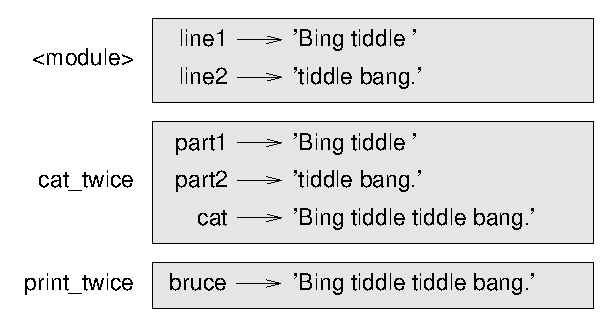
\includegraphics[scale=0.8]{figs/stack.eps}}
\caption{スタック図.}
\label{fig.stack}
\end{figure}
%
各仮引数は対応する引数が持つ値と同じものだ。だから、{\tt part1}は{\tt line1}と同じ値を参照しているし、
{\tt line2}も然りである。{\tt bruce}は{\tt cat}と同じ値を持つことになる。\par
関数呼び出しのときにエラーを起こすと、Pythonはその関数の名前、関数を呼んだ関数の名前、その前というように{\verb"__main__"}に至る全ての関数の名前を表示する。
例えば、関数{\tt print\_twice}内で{\tt cat}にアクセスしようとすると、{\tt NameError}になる：
\begin{verbatim}
Traceback (innermost last):
  File "test.py", line 13, in __main__
    cat_twice(line1, line2)
  File "test.py", line 5, in cat_twice
    print_twice(cat)
  File "test.py", line 9, in print_twice
    print(cat)
NameError: name 'cat' is not defined
\end{verbatim}
この関数のリストは{\bf トレースバック（traceback）}と呼ばれるものである。
これはプログラムのどこでこのエラーが発生したか、そして如何なる関数を実行しているときかといったことを示す。さらにこのエラーが起きたソースコードの行番号も示される。
このトレースバックに現れる関数はスタック図と同じ順序で示される。現在実行中の関数は一番下になる。\par
（訳注:上のトレースバックを発生させたスクリプトを以下に示す。ファイル名はtest.py：
\begin{verbatim}
01 def print_twice(bruce):
02    print(bruce)
03    print(bruce)
04    print(cat) #誤り
05
06 def cat_twice(line1, line2):
07    cat = line1 + line2
08    print_twice(cat)
09
10 #main
11 cat_twice('bono', 'niko')
\end{verbatim}
左端の行番号は便宜的に付けたものである。上のトレースバックはまずスクリプト{\tt test.py}の11行目のメイン（{\tt module}）で{\tt cat\_twice('bono', 'niko')}が実行され、次に8行の関数{\tt cat\_twice}内の {\tt print\_twice(cat)}が実行され、
次に4行目の関数{\tt print\_twice}内の{\tt print cat}でエラーが検出されたことを知らせている）
%
\section{結果を生む関数とボイド関数}
われわれが使っている関数、特に数学関数は結果を生む関数である。
適当な名前がないのでこれを{\bf 結果を生む関数（fruitful function）}と名付けることにする。{\tt print\_twice}のような関数は実行されても結果を返さないので、これは{\bf ボイド関数（void function）}と呼ばれている。 \par
関数を呼ぶというときには、何時も何か返すものを伴う実行がなされると期待するものである。
だからその結果をある変数に代入、表式の一部として使う。
\begin{verbatim}
x = math.cos(radians)
golden = (math.sqrt(5)+1)/2
\end{verbatim} \par
関数をインタラクティブ・モードで使うと、Pythonは結果を表示する：
\begin{verbatim}
>>> math.sqrt(5)
2.2360679774997898
\end{verbatim}
ところが、スクリプト・モードで結果を生む関数をそれ自体で呼ぶと、結果は永遠に失われてしまう：
\begin{verbatim}
math.sqrt(5)
\end{verbatim}
スクリプトは$５$の平方根を計算するが、保存し、表示する機能を持っていないので不便なことになる。\par
ボイド関数も画面に表示をし、似た効果をもたらすが戻り値がない。
その結果を変数で受け取ると、その値は{\tt None}という特別な値になる：
\begin{verbatim}
>>> result = print_twice('Bing')
Bing
Bing
>>> print(result)
None
\end{verbatim}
値{\tt None}は文字列{\tt 'None'}とは異なる。それはそれ自身の型をもつ特別な値である：
\begin{verbatim}
>>> type(None)
<class 'NoneType'>
\end{verbatim}
これまで作成した関数は全てボイド関数であった。これからの数章では結果を生む関数を書くことになる。
%
\section{なぜ関数？}
プログラムを関数に分割することに心を砕く理由はあまりはっきりとしないかもしれない。その理由としていくつかある。
\begin{itemize}
\item 関数を生成することで一括りの文に名前を付けることができ、読みやすく、デバッグし易いプログラムを作ることができる。
\item 関数化することで繰り返しをなくし、プログラムを短くすることができる。そして、何か変更が必要なことが起きたときには一個所を修正することで足りる。
\item 長いプログラムを関数に分割することで関数ごとのデバッグが可能になり、その後にそれらを全体して纏めることができる。
\item 良くできた関数は多くにプログラムで有用だ。一度書いてデバッグして完成させると、それを再利用することができる。
\end{itemize}
%
\section{デバッギング}
あなたが獲得しなければならない最も重要な能力の一つはデバッギングである。
デバッギングはやる気を挫くものであるが、これはプログラミングの作業のなかで最も知的で、やりがいがあり、興味深い領域である。\par
ある意味では、デバッギングは探偵の仕事に似ている。
幾つかの手懸かりを頼りにその結果を引き起こした過程やイベントを特定しなければならない。
また、デバッギングは実験科学に似ている。
何が間違っているかについて一つの考えが浮かんだら、プログラムを修正し、実行してみる。
この仮説が正しかったとすると、その変更の結果を予測てき、前に一歩進める。
仮説が間違っていたとすると、再度仮説を立て直さなければならない。
シャーロック・ホームズも指摘したように、「あなたが不可能を取り除いてしまったとき、
どんなものが残ろうとも、それがありそうもないことであっても、残ったものが真実にちがいない」（コナンドイル「四つの署名」）。\par
多くの人たちにとっては、プログラミングとデバッギングは同義語だ。
つまり、プログラミングとは最終的に欲しい結果を生み出すプログラムを徐々に完成させるデバッギングの過程である。
この考え方は、最初はほんの簡単なことができるプログラムを作成し、進捗するにつれて、
何時もその限りでは動くプログラムを心がけつつ、これを徐々に変更、デバッグするということだ。\par
例えば、Linuxはオペレーティング・システムの一つであり、ソースコードは数千行もあるプログラムであるが、Linus Torvaldsが嘗てIntel 80386チップの動きを調べるために作成した一つの簡単なプログラムであった。Larry Greenfieldによれば、
「Linuxの初期のプロジェクトの一つはprint AAAA と　print BBBBの切り替えを行うプログラムであった。
後にこれがLinuxへと進化した。」（The Linux Users’ Guide Beta Version 1）
%
\section{語句}
\begin{description}
\item[関数（function）：]意味のある命令を実行する文の纏まりに名前を付けたもの。関数は引数を取るものもあり、結果を返すものもある。
%\index{function}

\item[関数定義（function definition）：]関数名、仮引数、実行する文の纏まりを指定して新たな関数を作成するための文。  
%\index{function definition}

\item[関数オブジェクト（function object）：]関数定義で生成される一つの値。関数名はこの関数オブジェクトを参照する変数である。
%\index{function definition}

\item[ヘッダー（header）：]関数定義の一行目の部分。 .
:%\index{header}

\item[ボディー（body）：]関数定義の内部の本体（文の集合）。 
%\index{body}

\item[仮引数（parameters）：]関数の中で引数として渡される値を参照する変数。 
%\index{parameter}

\item[関数呼び出し（function call）：] 関数を実行する文。関数名と必要な実引数のリストが続く。
%\index{function call}

\item[引数（argument）：]関数が呼ばれたときその関数に付随して与えられる値。この値は関数の中では対応する仮引数に代入される。  
%\index{argument}

\item[ローカル変数（local）：]関数内で定義され使われる変数。ローカル変数はその関数内でのみ有効である。  
%\index{local variable}

\item[戻り値（return value）：]関数の結果。もし関数が表式として使われているとすると、その戻り値がその表式の値となる。 
%\index{return value}

\item[結果を生む関数（fruitful function）：]結果を返す関数。 
%\index{fruitful function}

\item[ボイド関数（void function）：]値を返さない関数。 
%\index{void function}

\item[モジュール（module）：]関連する関数群や付随する定義を一つに纏めたファイル。 
%\index{module}

\item[インポート文（import statement）：]一つのモジュールを読み込みモジュール・オブジェクトを生成する文。 
%\index{import statement}
%\index{statement!import}

\item[モジュール・オブジェクト（module object）：] 一つのモジュール内で定義されている値へのアクセスを提供する{\tt import} 文が生成する値。
%\index{module}

\item[ドット表記（dot notation）：]  他のモジュールに属する関数や定義を使うとき、
それらをモジュール名に続いてピリオドそして関数名（または定義変数）で指定する構文規則。
%\index{dot notation}

\item[混合（composition）：]より長い表式の一部として表式を、またはより複雑な文の一部として文を使うこと。 
\index{composition}

\item[実行の流れ（flow of execution）：]プログラムの実行時にどの文から実行されるかの順序。 .
%\index{flow of execution}

\item[スタック図（fig.stack）：]  一つのモジュールで使われる関数群やそれらの内部で定義される変数、
そしてそれらの変数が参照する値の対応を表示するグラフィカルな表現。
%\index{fig.stack}

\item[フレーム（frame）：]スタック図内で関数呼び出しを表現する枠。  
%\index{function frame}
%\index{frame}

\item[トレースバック（traceback）：]例外が発生したときに表示される実行されていた関数のリスト。
%\index{traceback}

\end{description}

\section{練習問題}
\noindent
{\bf 練習問題\tp.1}　Pythonは文字列の長さを返す組み込み関数{\tt len}、例えば{\tt len('allen')}は{\tt 5}を返す、を提供している。\par
文字列の表示で、文字列の最後の文字が70桁にくるような{\tt right\_justify}関数を作成せよ。
\begin{verbatim}
>>> right_justify('monty')
                                                                 monty
\end{verbatim}  

\noindent                                                                 
{\bf 練習問題\tp.2}　関数オブジェクト自体も関数の引数とすることができる。
例えば、{\tt do\_twice}関数は関数オブジェクトを引数として受け取りその関数を二度実行する、つまり
\begin{verbatim}
def do_twice(f):
    f()
    f()
\end{verbatim}      
さて、{\tt do\_twice}が以下の関数{\tt print\_spam}を引数とする使用例をみてみよう：
\begin{verbatim}
def print_spam():
    print('spam')

do_twice(print_spam)
\end{verbatim}   
この関数を以下の順序を踏んで変更せよ：
\begin{enumerate}
\item 上記のプログラムをスクリプトとして書き、実行せよ。
\item 引数を二つ持つように{\tt do\_twice}を変更せよ。一つの引数は関数オブジェクトであり、他はこの関数が受け取る引数の値である。
\item {\tt print\_spam}をより一般的な関数{\tt print\_twice}に変更せよ。この新しい関数は引数を一つ持ち、それを二回表示する。
\item 新しい関数{\tt do\_four}を作成せよ。この関数は関数オブジェクトを引数の一つとし、
他の引数はこの関数が引数として受け取る値である。この新しい関数は引数として受け取った関数を四回実行する。
この新しい関数の本体は二つの文で書ける。四つではないよ。\par
\end{enumerate}
解答例：\url"http://thinpython.com/code/do\_four.py"

\noindent
{\bf 練習問題\tp.3}　この練習問題はこれまで学んだ文や他の機能を使って解答できるものである。\par
１．以下のような格子を描く関数を作成せよ。
\begin{verbatim}
+ - - - - + - - - - +
|         |         |
|         |         |
|         |         |
|         |         |
+ - - - - + - - - - +
|         |         |
|         |         |
|         |         |
|         |         |
+ - - - - + - - - - +
\end{verbatim}  
ヒント：{\tt print}文で一つ以上の値を一時に表示したいときは、値をカンマで区切ったもので{\tt print}とするとよい：
\begin{verbatim}
print('+','-')
\end{verbatim}
また通常は{\tt print}文は行の終わりに段落（{\verb"\n"}）を吐いて次の行に移るが、この動きを無効にして例えば
空白を吐いて終わりにすることもできる：
\begin{verbatim}
print('+', end=' ')
print('-')
\end{verbatim}
この出力は{\tt '+ -'}である。 \par
{\tt print}文それ自体で行が終わったら、改行で次ぎに行に移る。 \\

2.	同様に四行四列の格子を描く関数を作成せよ。\\
解答例：\url"http://thinpython.com/code/grid.py"。\\
出典：この練習問題はOualline著"Practical Programming. Third Edition ( O'Relly Media, 1997)"の中の練習問題を基礎とした。
%
\chapter{事例研究：インタフェース設計}
この章はインタフェース設計のための諸機能を取り入れる過程を紹介する事例研究である。　\par
まず{\tt turtle}モジュールを導入しよう。このモジュールを使うと{\tt turtle}グラフィックスで描画を作成できる。
{\tt turtle}モジュールは大抵のPythonのインストール・パッケージに含まれているはずだ。
{\tt PythonAnywhere}を使ってPythonを起動しているばあいには{\tt turtle}は動かないかもしれいない。\par
Pythonをインストールしてあるのであれば、ここのサンプルプログラムは動くはずだ。そうでなければ
インストールのよい機会である。仕方はに別途\url{http://tinyurl.com/thinkpython2e}.に纏めておいた。\par
この章のサンプルコードは\url{https://thinkpython.com/code/polygon.py}にある。
%
\section{{\tt turtle}モジュール}
{\tt turtle}モジュールがインストールされているか確認するためにPythonインタプリタを起動して以下を入力
してみよう。
\begin{verbatim}
>>> import turtle
>>> bob = turtle.Turtle()
\end{verbatim}
これでカメを意味する小さい矢印が表示された新しい窓が現れるはずだ。確認できたら窓を閉じる。\par
さて、スクリプトモードで以下のコードを入力し{\tt mypolygon.py}と言う名前のファイルとして保存する：
\begin{verbatim}
import turtle
bob = turtle.Turtle()
print(bob)
turtle.mainloop()
\end{verbatim}
{\tt turtle}モジュール（{\tt t}は小文字）は{\tt Turtle}オブジェクトを生成する{\tt Turtle}（{\tt T}は大文字）関数
{\tt Turtle}を含んでいる。ここではこのオブジェクトは変数{\tt bob}に代入されている。この{\tt bob}を表示すると
以下のようなものだ出るはずだ：
\begin{verbatim}
<turtle.Turtle object at 0xb7bfbf4c>
\end{verbatim}
これは変数{\tt bob}は{\tt turtle}モジュールで定義されている{\tt Turtle}型のオブジェクトを参照しているという
意味だ。\par
{\tt mainloop}は{\tt window}に対してユーザが何か動作するのを待つようにと通知していることだ。もっとも
今のばあいにユーザのできることは窓を閉じることぐらいしかないが。\par
一度{\tt Turtle}を生成していおくと、このカメ（今のばあいは{\tt bob}）をこの窓の中で動かす{\bf メソッド（method）}を呼び出す
こができる。メソッドは関数に似ているが、少し異なった構文を使う。例えばカメを前進させるには：
\begin{verbatim}
bob.fd(100)
\end{verbatim}
%
このメソッド{\tt fd}は{\tt Turtle}オブジェクトである{\tt bob}に付随しているものである。
メソッドを呼ぶということは要請するようなものだ。{\tt bob}に前に進むことを要請したわけである。\par
{\tt fd}の引数はピクセル単位の距離であり、実際の長さは使っているディスプレーによる。\par
{\tt Turtle}に対して呼び出すことができるその他のメソッドには後退{\tt bk}、左回転{\tt lt}そして
右回転{\tt rt}がある。メソッド{\tt lt}と{\tt rt}の引数は度を単位とした角度である。\par
また各{\tt Turtle}はペンを保持していて、それを上げたり下げたりする。
それが下がっていると、{\tt Turtle}は動くにつれて軌跡を画面に描く。メソッド{\tt pu}と{\tt pd}
は「ペンを上げ」、「ペンを下げ」のつもりである。\par
直角を描くために以下の行をプログラムに追加してみよう（追加する場所は{\tt bob}の生成の後で、{\tt mainloop}の前である）。
\begin{verbatim}
bob.fd(100)
bob.lt(90)
bob.fd(100)
\end{verbatim}
このプログラムを実行すると、{\tt bob}は東に向いて前進し、その後北向きに進路を取り、直角を成す二つの線分が
画面にできる。\par
このプログラムを変更して、正方形を描いてみよう。上手く行くまで続けてみよう。
%
\section{簡単な繰り返し}
多分あなたが行った変更は以下のようなものはずだ：
\begin{verbatim}
bob.fd(100)
bob.lt(90)

bob.fd(100)
bob.lt(90)

bob.fd(100)
bob.lt(90)

bob.fd(100)
\end{verbatim} \par
これは{\tt for}文を使うともっとコンパクトに書ける。
これらを{\tt mypolygon.py}に追加して実行してみよう。
\begin{verbatim}
for i in range(4):
    print('hello!')
\end{verbatim}
得られる結果は以下である：
\begin{verbatim}
hello!
hello!
hello!
hello!
\end{verbatim}
これは簡単な{\tt for}文の利用法である。詳細は後にみることにする。
正方形を描くプログラムに{\tt for}文を使うのには、上の例題で充分だ。 試してみよう。\par
以下は正方形描画の{\tt for}文版だ。
\begin{verbatim}
for i in range(4):
    bob.fd(100)
    bob.lt(90)
\end{verbatim}　\par
{\tt for}文の構文は関数定義と似ている。コロンで終わるヘッダーを持ち、インデントされたボディからなる。ボディは任意の数の文を含んで構わない。
{\tt for}文は{\bf ループ（loop）}と呼ばれる。
実行の流れがボディを実行してあとボディのトップに戻るからである。今の場合はボディを4回繰り返す。\par
この{\tt for}文を使った正方形描画プログラムはオリジナルのものとホンの僅かだが異なっている。
それは正方形を描いた後、{\tt bob}が余計な左転回をすることだ。\par
この{\tt for}文版は指摘したように最後の左回転が余分である。これが実行時間に影響するかもしれないが、同じことをループを
使って書けることでコードを簡素にすることができる。またこの版ではループを終えたときにはカメはループに入る前の方向を向いて
いる効果も持っている。
%
\section{練習問題}
以下は{\tt TurtleWorld}を使った練習問題のシリーズである。
それらは面白いものであるが、学習のポイントも含まれている。作業をしながらその学習ポイントにも目を向けてほしい。\par
以下の節でその解答を提示するが、完成するまで（少なくも試みるまで）はそれをみてはいけない。
\begin{enumerate}
\item squareという関数を作成せよ。仮引数として{\tt turtle}である{\tt t}を持つ。
この{\tt turtle}で正方形を描くようにせよ。そしてこの関数で{\tt bob}を引数として受け取り関数呼び出しを書き実行せよ。

\item {\tt length}という別な仮引数を追加せよ。関数のボディを変更してlengthを一辺の長さにするように変更し、
関数呼び出しに第二の引数を持つように変更せよ。適当な長さの{\tt length}を与え実行してみよう。

\item 関数ltの回転角度の既定値は{\tt 90}である。しかし、{\tt lt(bob, 45)}のように角度を与えることもできる。
そこで{\tt square}をコピーして名前を{\tt polygon}とする。この関数は第二の仮引数nを持ち、ボディをn個の辺を持つ正多角形を描くように変更せよ。\par
ヒント：{\tt n}個の辺を持つ正多角形の外角は{\tt 360/n}である。

\item {\tt circle}関数を作成せよ。この関数は{\tt polygon}関数から派生し、
仮引数として{\tt turtle}を値に持つtと、半径{\tt r}を持ち、近似的に円を描く関数である。\par
ヒント：円周は近似的に正{\tt n}辺多角形で近似すると、円周　{\tt = length * n}で表現できる。ここで{\tt length}は多角形の一辺の長さである。 \par
もう一つヒント：描画速度が余りのも遅いときは、{\tt bob,delay = 0.01}とするとよい。

\item 更に一般的な関数{\tt arc}関数を作成せよ。この関数は追加の仮引数として{\tt angle}を持つ。描画はこの{\t angle}を角度とする孤を描くことにある。{\tt angle = 360}で完全な円を描くことになる。
\end{enumerate}
%
\section{カプセル化}
第一例は正方形を描画するコードを関数にする問題である。この関数の呼び出しでは{\tt Turtle}オブジェクトを引数として
渡すようにする。解答例は
\begin{verbatim}
def square(t):
    for i in range(4):
        t.fd(100)
        t.lt(90)

square(bob)
\end{verbatim}
%
最も内側の{\tt fd}と{\tt lt}は二段にインデントされる。
これらは関数定義のボディの始まりである{\tt for}ループの内部にある。
次の行にある{\tt square(bob)}は左余白をなくして入力される。このことは{\tt for}ループも関数定義も終了したことを意味する。\par
関数の内部では{\tt t}は同一の{\tt turtle}である{\tt bob}を参照しているから、{\tt lt(t)}は{\tt lt(bob)}と同じ効果を持つ。
それならば、何故直接{\tt bob}を呼ばないのか？
これは関数{\tt square}ではtはどんな{\tt turtle}にもなり得るからだ。
二匹目の{\tt turtle}を作成し、それをこの関数の引数にすることもできる、つまり：
\begin{verbatim}
alice = turtle.Turtle()
square(alice)
\end{verbatim}
コードの一部を関数として纏める作業を{\bf カプセル化（encapsulation）}と呼ぶ。
カプセル化の利点は関数名としてコードに名前がつくのでドキュメントとなること。
もう一つの利点はコードを再利用したいとき、関数呼び出しで事足りることである。
%
\section{一般化}
次ぎのステップは{\tt square}関数に仮引数{\tt length}を追加することである。解答例は
\begin{verbatim}
def square(t, length):
    for i in range(4):
        t.fd(length)
        t.lt(90)

square(bob, 100)
\end{verbatim}
関数に仮引数を追加する作業を{\bf 一般化（generalization）}という。 この作業で関数はさらに一般化される。\par
次ぎのステップも一般化で、正方形を描画する替わりに、正多角形を描画するものである。解答例は以下である：
\begin{verbatim}
def polygon(t, n, length):
    angle = 360 / n
    for i in range(n):
        t.fd(length)
        t.lt(angle)

polygon(bob, 7, 70)
\end{verbatim}
{\tt 7}辺を持ち、一辺の長さが{\tt 70}の正多角形を描画する。\par
Python2を使っているとすると、角度の値が整数の割り算に伴なう打ち切り誤差を生じるかもしれない。簡単な解決は
{\tt  angle = 360.0/ n}とすることだ。分子が浮動小数点数であるので結果も浮動小数点数になるからだ。\par
もし引数の数が増えて、その数値の意味が曖昧になり、順序が不明になったときは、仮引数の名前を付して引数を書くことは合法である：
\begin{verbatim}
polygon(bob, n=7, length=70)
\end{verbatim}
これは{\bf キー付き引数（keyword argument）}という。この構文規則はプログラムをより読みやすくする。
%
\section{インタフェース設計}
次ぎのステップは半径rを仮引数として円を描画する関数の作成の問題である。以下は{\tt 50}辺を持つ多角形を描画する解答の一例である：
\begin{verbatim}
def circle(t, r):
    circumferance = 2 * math.pi * r
    n=50
    lenght = circumferance / n
    polygon(t, lenght, n)
 \end{verbatim}   
第一行では円の円周を計算している。$\pi$の値は数学モジュールで与えられるので、{\tt math}モジュールのインポートを忘れないように。
慣例として{\tt import}文はプログラムの先頭に置く。\par
{\tt n}は多角形の辺の数であり、この多角形で半径{\tt r}の円を近似的に描画することができることを使う。\par
この解答例の問題点は{\tt n}が定数であることである。
これでは大きな円では一辺の長さが大きくなって円の近似としては粗くなる。逆に、小さな円では一辺が小さくなりすぎて描画時間が無駄になる。
{\tt n}を仮引数にすることも一案だが、インタフェースとしては明確さを欠くことにある。\par
関数の{\bf インタフェース（inteface）}とはその関数の使い方の指針である：
「仮引数は何か？」、「この関数は何をする関数か？」、「戻り値は何か？」について纏めたものである。
そのインタフェースは明確であるということは、「可能なかぎり簡単で、簡単すぎることもない」（アインシュタイン）ことである。\par
今の例では、{\tt r}は描画しようとする円の半径の値を特定するものであるのでインタフェースに属すると考えられる。
しかし、{\tt n}は如何に円を描画するかに使うものなので、そうではない。
これはインタフェースを乱雑にするだけなので、むしろ関数のボディのなかで円周から計算する方がよい。
\begin{verbatim}
def circle(t, r):
    circumference = 2 * math.pi * r
    n = int(circumference / 3) + 3
    length = circumference / n
    polygon(t, n, length)
\end{verbatim}
これで一辺の数は{\tt circumferance/3}になり、一辺の長さは約{\tt 3}になる。
これはできる多角形で充分に円を近似できる最小で、しかも大きな円でも充分な数である。
これで如何なる大きさの円の描画に使える関数ができたことになる。
%
\section{再因子分解\label{arc}}
円の描画では関数{\tt polygon}を再利用できた。これは正多角形が円の近似になるからである。
しかし、円弧を描画しようとすると{\tt polygon}も{\tt circle}も使えない。 \par
一つの解決方法は関数{\tt polygon}のソースコードをコピーして、直接に関数{\tt arc}に加工するものである。結果は以下のようになる：
\begin{verbatim}
def arc(t, r, angle):
    arc_length = 2 * math.pi * r * angle / 360
    n = int(arc_length / 3) + 1
    step_length = arc_length / n
    step_angle = angle / n
    
    for i in range(n):
        t.fd(step_length)
        t.lt(step_angle)
\end{verbatim}
後半は関数{\tt polygon}に似た処理をしているが、{\tt polygon}を書き換えないと使えない。
そこで、{\tt polygon}を第三の引数を持たせるように書き換えることにする。名前も{\tt polyline}とする：
\begin{verbatim}
def polyline(t, n, length, angle):
    for i in range(n):
        t.fd(length)
        t.lt(angle)
\end{verbatim}
この新しく定義された関数は{\tt polygon}にも使えるし、{\tt arc}にも使える。{\tt polygon}は以下のようになる：
\begin{verbatim}
def polygon(t, n, length):
    angle = 360.0 / n
    polyline(t, n, length, angle)
\end{verbatim}
関数arcは以下のようになる（訳注：ここでの{\tt angle}は円弧を見込む角度）：
\begin{verbatim}
def arc(t, r, angle):
    arc_length = 2 * math.pi * r * angle / 360
    n = int(arc_length / 3) + 1
    step_length = arc_length / n
    step_angle = float(angle) / n
    polyline(t, n, step_length, step_angle)
\end{verbatim}

円周は円弧の特別な形なので、関数{\tt circle}は関数{\tt arc}で書くことができる：
\begin{verbatim}
def circle(t, r):
    arc(t, r, 360)
\end{verbatim} \par
以上のような過程、つまり関数インタフェースを改良し、コードの再利用を促進する方法を{\bf 再因子分解（refactoring）}という。
いまの場合は関数{\tt arc}と関数{\tt polygon}とに共通する部分があり、この共通項として関数{\tt polyline}を「抽出」したことになる。\par
最初からこのことが分かっていたら、関数{\tt polyline}から始めたかもしれない。
しかし、多くの場合プロジェクトの最初から全ての関数インタフェースを設計しておくことは難しい。
プログラムを書き始めて問題が良く理解できるものである。
ときとして再因子分解をしようと思うことは問題をよりよく理解できたサインである。
%
\section{開発計画}
{\bf 開発計画（development plan）}はプログラムを書く過程のことである。
この過程としてわれわれがみてきたものは、「カプセル化と一般化」である。この過程は以下のように纏められる：
\begin{enumerate}
\item まず、関数を使わないで小さいプログラムを書く。
\item プログラムは実行できるようになったら、それを関数としてカプセル化し、名前を付ける。
\item 適宜仮引数を追加してそれを一般化する。
\item １～3を繰り返し、プログラムが動くようにする。
\item 再因子分解でプログラムが改良できるかコードを眺めてみる。
例えば、プログラムの中に同じようなコードを使っている個所あれば、適当な関数でそれらを置き換える。
\end{enumerate}
この過程は欠点もあるが、もしプログラムをどのような関数に分解したらよいか事前に分からないときには助けになる（後に別なアプローチを示す）。
この方法はプログラミングを進めながら設計も進める方法である。
%
\section{ドキュメント文字列}
{\bf ドキュメント文字列（docstring）}とは関数のインタフェースを説明するために関数の初めの部分に置く文字列のことである（``doc"は
``documentation"の省略）。例を示す。
\begin{verbatim}
def polyline(t, n, lenght, angle):
    """与えられた長さ（lenght）と与えられた線分間
    角度（angle）（度）を持つn個の線分を描画する。
    tはturtleである。"""
    
    for i in range(n):
        t.fd(length)
        t.lt(angle)
\end{verbatim}
この文字列は三重の引用符で括られている。三重の引用符は複数行に渡る文字列を書くことができるからだ。\par
この例のようにドキュメント文字列は短いがこの関数を使おうとしたときに必要な情報を含んでいる。
これは簡潔にこの関数の機能が関数の細部に渡らずに説明されているし、仮引数の役割（時には型についても）も示されている。\par
このようなドキュメントを書くことは関数のインタフェースの設計の重要な部分である。
良く設計されたインタフェースは説明も明快にできるはずである。
もし関数のインタフェースの説明に苦労するようであれば、
それは多分にインタフェース自体の改良が必要なサインであり得る。
%
\section{デバッギング}
インタフェースは関数とその呼び手との接面のようなものである。
呼び手は仮引数に対して値を与えることに同意し、関数はそれをもとに作業をすることに同意する。\par
例としてみると、{\tt polyline}は四個の引数を要求している。
{\tt t}は{\tt turtle}、{\tt n}は線分の数、従って整数、{\tt length}は線分の長さ、だから正の数値、{\tt angle}は度を単位とする数値である。\par
これらの要求は{\bf 事前条件（precondition）}という。
関数が実行される前に実現しておく必要のある条件だからである。この逆に、
関数の終わりで示される条件は{\bf 事後条件（postcondition）}と言われるものである。
これにはその関数が意図したもの（線分の描画のような）、
その関数の実行による副産物（{\tt turtle}の移動、世界に及ぼす変更のような）が含まれる。\par
事前条件は呼び手が責任を負うものである。
呼び手がこの事前条件に反し、関数が正常に働かないとすると、バグは呼び手にあり、関数ではない。
%
\section{語句}
\begin{description}

\item[メソッド（method）：] オブジェクトに付随している関数、そしてドット表記で呼ばれる。
%\index{method}

\item[ループ（loop）：]繰り返して実行されるプログラムの部分。 
%\index{loop}

\item[カプセル化（encapsulation）：]一つの目的のための一連の文の集合を一つの関数として変形する過程。.
%\index{encapsulation}

\item[一般化（generalization）：]必要なく特定されているもの（例えば数）を適当な一般的なもの（変数や仮引数）に置き換える過程。
%\index{generalization}

\item[キー付き引数（keyword argument）：]「キー」として仮引数の変数名を含めた実引数
%\index{argument!keyword}

\item[インタフェース（inteface）：] 関数名、引数や戻り値の説明を含めたその関数の使い方に関する叙述。
%\index{interface}

\item[再因子分解（refactoring）：]関数のインタフェースやコードの質的な向上のため作動しているプログラムを改変する過程。
%\index{refactoring}

\item[開発計画（development plan）：]プログラムを作成する過程。
%\index{development plan}

\item[ドキュメント文字列（docstring）：] 関数定義の中で 関数のインタフェースを叙述した文字列。
%\index{docstring}

\item[事前条件（precondition）：] 関数を呼ぶ前に呼び手が満たすべき条件。
\index{precondition}

\item[事後条件（postcondition）：] 関数の実行が終わった時点でその関数が満たすべき条件。
%\index{precondition}
\end{description}
%
\section{練習問題}
\noindent
{\bf 練習問題\tp.1}　\url{https://thinkpython.com/code/polygon.py}をダウンロードし以下の課題を行え。
\begin{enumerate}
\item 関数{\tt circle(bob, radius)}の実行に伴うスタック図を作成せよ。手書きでもよいし、コードに{\tt print}文で追加してもよい。

\item \ref{arc}節の関数arcは、円の描画が常に想定した円の外側に沿った線分で近似されているので正確さに欠けるところがある。
その結果{\tt turtle}が停止した位置は正しい位置から僅かにずれる。
わたしの解答例ではこの誤差を減ずる工夫がされている。コードを読んで納得できるがみよ。図を描いてみるとそれが有効である
ことが分るかもしれいない。
\end{enumerate}
%
\begin{figure}[H]
\centerline
{
\includegraphics[scale=0.8]{figs/flowersA.eps}}
\caption{タートルの花々}
\label{fig.flowers}
\end{figure} 

\noindent
{\bf 練習問題\tp.2}　図\ref{fig.flowers}のような描画に対応する関数の典型的なセットを作成せよ。\\
解答例：\url{https://thinkpython.com/code/flower.py}　
及び\url{https://thinkpython.com/code/polygon.py}.も必要である。
 
\noindent
{\bf 練習問題\tp.3}　図\ref{fig.pies}のような描画に対応する関数の典型的なセットを作成せよ。\\
解答例：\url{https://thinkpython.com/code/pie.py}.
%
\begin{figure}[H]
\centerline
{
\includegraphics[scale=0.8]{figs/piesA.eps}}
\caption{タートルのパイ}
\label{fig.pies}
\end{figure}

\noindent
{\bf 練習問題\tp.4}　アルファベットの文字は適当な数の基本要素、つまり横線、縦線、いくつかの曲線から生成できる。
フォントをこのような要素から作れるようデザインせよ。そして、アルファベットを描画する関数を作成せよ。\par
先ず、各一文字を描画する関数を生成する。つまり、{\tt draw\_a}、{\tt draw\_b}といった具合である。
これらを纏めて{\tt letters.py}というファイルにする。あなたの制作した関数をテストするために
``turtle typewriter"というモジュールを \url{https://thinkpython.com/code/typewriter.py}
からダウンロードせよ。\\
解答例：\url{https://thinkpython.com/code/letters.py}
及び\url{https://thinkpython.com/code/polygon.py}.も必要である。

\noindent
{\bf 練習問題\tp.5}　渦巻について、
\url{http://en.wikipedia.org/wiki/Spiral}（訳注：日本語では\url{http://ja.wikipedia.org/wiki/渦巻}）の記事をよみ、アルキメデスの渦巻（または、類似の渦巻）を描画するプログラムを作成せよ。\\
解答例：\url{https://thinkpython.com/code/spiral.py}."
%
\chapter{条件文と再帰}
この章の主なテーマはプログラムの状態に依存して異なったコードを実行する{\tt if}文である。しかしその前に新たな二つ演算子、打ち切り除算、モジュラ演算子
を導入したい。
\section{打ち切り除算とモジュラ演算子}
{\bf 打ち切り除算（Floor division）}（演算子は{\verb"//"}）は二つの数値の除算で結果の小数点以下を負の無限大の方向に丸める演算である。
例として一つの映画
の上演時間が105分であったとしよう。これが時を単位にすると幾らになるか知りたいと思ったとしよう。従来の除算では浮動小数点数が得られる：
\begin{verbatim}
>>> minutes = 105
>>> minutes / 60
1.75
\end{verbatim}
時は通常は小数点を付けては使わない。打ち切り除算は小数点以下を切り捨て整数として時を表示する：
\begin{verbatim}
>>> minutes = 105
>>> hours = minutes // 60
>>> hours
1
\end{verbatim}
残りは全体から一時間を分にしたものを引き算すると出せる：
\begin{verbatim}
>>> remainder = minutes - hours * 60
>>> remainder
45
\end{verbatim}
他の方法は{\bf モジュラ演算子（modulus operator）}を使う。
これは整数に対する演算子で、最初の被演算子を二番目の被演算子で除算したときの余りを生成するものである。
Pythonではこの演算子は{\verb"%"}で表現される。構文は他の演算子と同じである：
\begin{verbatim}
>>> remainder = minutes % 60
>>> remainder
45
\end{verbatim}
モジュラ演算子は極めて有用なものであることが分かってくる。例えば、ある整数が他の整数で割り切れるか調べたいときには、
{\verb"x % y"}
がゼロならば、{\tt x}が{\tt y}で割り切れるということになる。 \par
また、ある整数に一桁目の数字や下何桁かの数字を求めたときにも使える。例えば、{\verb"x % 10"}
とすると、整数{\tt x}の十進一桁目の数字が、{\verb"x % 100"}
で下二桁の数字が得られる。\par
Python2を使っているとすると除算は異なった結果になる。除算の演算（演算子は{\verb"/"}）はもしも被演算子が
二つとも整数値であると打ち切り除算になり、被演算子のどちらかが浮動小数点数であると結果も{\tt float}型になる。
%
\section{ブール代数表現}
{\bf ブール代数表現（boolean expression）}は{\bf 真（true）}と{\bf 偽（false）}の表現である。
以下の例では、演算子{\tt ==}を使い二つの被演算子を比較し、等しい場合は真をそれ以外は偽を値として持つ。
\begin{verbatim}
>>> 5 == 5
True
>>> 5 == 6
False
\end{verbatim}
{\tt True}と{\tt False}は{\tt bool}型に属する特別な値である。これらは文字列ではない：
\begin{verbatim}
>>> type(True)
<class 'bool'>
>>> type(False)
<class 'bool'>
\end{verbatim}　\par
演算子{\tt ==}は{\bf 比較演算子（relational operators）}の一つであり、他の演算子としては
\begin{verbatim}
x != y    #xはyに等しくない
x > y	    #xはyより大きい
x < y	    #xはyより小さい
x >= y    #xはyより大きいが等しい
x <= y    #xはyより小さいか等しい
\end{verbatim}
これらの演算子は数学的な記号として馴染み深いものであるが、Pythonでの記号の意味はそれらと若干異なる。
もっともよくある間違いは二重等号（{\tt ==}）の替わりに、等号（{\tt =}）を使ってしまうことだ。
記号{\tt =}は代入演算子であり、記号{\tt ==}が比較演算子である。また、{\tt =>}や{\tt =<}はない。
%
\section{論理演算子}
三つの{\bf 論理演算子（logical operators）}、{\tt and}、{\tt  or}、 {\tt not}がある。これらの意味はその英語の意味に似ている。例えば、
{\tt x > 0 and x < 10}は{\tt x}が{\tt 0}より大きく、かつ{\tt 10}より小さいとき真の値を持つ。
{\verb"x % 2 == 0 or x%3 == 0"}
はどちらかの条件が満たされると真の値を持つ。
つまり、ある数が{\tt 2}か{\tt 3}かで割り切れればよい。
最後は{\tt not}でブール代数の否定演算子である。{\tt not (x > y)}は、{\tt x > y}が偽のとき真、つまり{\tt x}が{\tt y}より小さいか等しいときである。\par
厳密に言って、論理演算子の被演算子は論理表式であるべきだが、Pythonはそう厳密ではない。非ゼロの如何なる数値も論理的に真と解釈する。
\begin{verbatim}
>>> 42 and True
True
\end{verbatim}
この柔軟性は有用であるが、混乱を引き起こす微妙な違いがある。このような使い方は避けた方がよい（何が起きているか把握できるまでは）。
%
\section{条件処理}
有用なプログラムを書くためにはわれわれは条件を調べ、それに従ってプログラムの振る舞いを替える機能が必要になる。{\bf 条件文（conditional statement）}はそのような機能である。このif文の極簡単な例は
\begin{verbatim}
if x > 0:
    print('x is positive')
\end{verbatim}
{\tt if}の後のブール代数表式は{\bf 条件（condition）}と呼ばれる。それが真であると、インデントされた文が実行され、そうでないと実行されない。\par
条件文は関数の定義と同じ構造をしている。つまり、インデントされたボディを従えたヘッダー。このような文を{\bf 複合文（compound statements）}という。ボディは無制限の数の文があってもよいが、最低でも一文は必要である。
ときとして文なしのボディが必要なときがある（大抵の場合これはまだ書き終えていない部分を余白として残したいときだ）。このようなときは何もしない{\tt pass}文を使うとよい：
\begin{verbatim}
if x < 0:
    pass     #負の場合の処理が必要
\end{verbatim}
%
\section{二者選択処理}
{\tt if}文の二番目のかたちは{\bf 二者選択処理（alternative execution）}である。
これでは二つ可能性があり、条件はどっちを取るかを決める。構文は以下のようだ：
\begin{verbatim}
if x%2 == 0:
    print('x is even')
else:
    print('x is odd')
\end{verbatim}
条件は真または偽のはずなので、二者の内の一つは必ず実行される。
二者択一は、実行の流れの分岐であるから、{\bf 分岐処理（branches）}とも言われる。
%
\section{条件文の連鎖}
ときとして二つ以上の可能性がある場合があり、二つ以上の分岐が必要となる。
このような処理を表現する一つの方法は{\bf 条件文の連鎖（chained conditional）}を使うものがある：
\begin{verbatim}
if x < y:
    print('x is less than y')
elif x > y:
    print('x is greater than y')
else:
    print('x and y are equal')
\end{verbatim}
{\tt elif} は　``else if"の省略形である。
ここでも一つの分枝が必ず実行される。{\tt elif}文の個数には制限がない。
{\tt else}節を使うときはこれを最後に置く。これがある必要もない。
\begin{verbatim}
if choice == 'a':
    draw_a()
elif choice == 'b':
    draw_b()
elif choice == 'c':
    draw_c()
\end{verbatim}   
各条件は順次調べられる。もし初めが偽であるとすると、次ぎが調べられという具合である。
それらの一つが真であるとその分枝が実行され、文の終わりになる。一つ以上の真があっても初めの真の分枝が実行されるだけである。
%
\section{入れ子の条件処理}
条件処理は入れ子にできる。三分枝の例題は以下のようになる：
\begin{verbatim}
if x== y:
    print('x and y are equal')
else:
    if x < y:
        print('x is less than y')
    else:
        print('x is greater than y')
\end{verbatim}  
外側の条件文には二つの分枝がある。一つの分枝は単純な一つの文からなるが、他の文枝はもう一つのif文からなる。
このif文は二つの分枝がある。それぞれの分枝はまた条件文だということもあり得るが、今回は各分枝とも単純な一つの文である。
インデントされた文の構造から{\bf 入れ子の条件処理（nested conditionals）}は読みやすいとは言えないので、なるべく避けるようにしたい。\par
論理演算子はこのような入れ子の条件処理を単純な処理に替えることができる。
例として以下のプログラムは１つの条件文に書き替えることができることを示す：
\begin{verbatim}
if 0 < x:
    if x < 10:
        print('xは一桁の整数である')
\end{verbatim} 
{\tt print}文は二つの条件文を通過したときのみ実行される。これは論理積演算子{\tt and}を使うと簡潔に表現できる：
\begin{verbatim}
if 0 < x and x > 10:
    print('xは一桁の整数である')
\end{verbatim}
%
\section{再帰\label{recursion}}
一つの関数が他の関数を呼ぶことは合法であるが、自分自身を呼ぶことも合法だ。
このようなことで何か得なことがあるとは俄には信じられないが、これはプログラムで実現できる魔法のような世界であることが徐々に明らかになる。 \par
例として以下のようなプログラムを眺めてみよう：
\begin{verbatim}
def countdown(n):
    if n == 0:
        print('Blastoff!')
    else:
        print n
        countdown(n-1)
\end{verbatim}       
{\tt n}が{\tt 0}か負になるとBlastoff!（発射！）'を{\tt print}する。
それ以外は{\tt n}を表示し、引数を{\tt n-1}として関数{\tt countdown}、つまり自分自身を呼ぶ。\par
{\tt main}関数でこの関数を以下のように呼んだら何がおきるだろう：
\begin{verbatim}
>>> countdown(3)
\end{verbatim}
関数countdownはn=3から始まる。nの値が0より大きいので、nの値3をprintして自分自身を呼ぶ。
\begin{quote}
関数countdownはn=2で実行される。nの値が0より大きいので、nの値2をprintして自分自身を呼ぶ。
\begin{quote}
関数countdownはn=1で実行される。nの値が0より大きいので、nの値1をprintして自分自身を呼ぶ。
\begin{quote}
関数countdownはn=0で実行される。nの値が0に等しいので、”Blastoff!”をprintして、関数をreturnする。\\
n=1のcountdownが関数returnに達する。
\end{quote}
n=2のcountdownが関数returnに達する。
\end{quote}
n=3のcountdownが関数returnに達する。
\end{quote}
%
そして{\tt main}関数{\verb"__main__"}に戻る。従って全表示は以下のようになる：
\begin{verbatim}
3
2
1
Blastoff!
\end{verbatim}
自分自身を呼ぶ関数は再帰的で、このプロセスを{\bf 再帰処理（recursion）}という。 \par
もう一つの例は文字列を表示するプログラムである：
\begin{verbatim}
def print_n(s, n):
    if n <= 0:
        return
    print(s)
    print_n(s, n-1)
\end{verbatim}
もし{\tt n <= 0}であるとすると、
関数{\tt return}が実行される。実行は呼び出し関数に戻ることである。
この関数の残りの部分は{\tt countdown}に類似している。
{\tt n}が{\tt 0}より大きいと文字{\tt s}を{\tt print}し、
残りの{\tt (n-1)}回の{\tt print}のために自分自身を呼んでいる。
従って、文字{\tt s}の{\tt print}は{\tt 1 + (n-1)},つまり{\tt n}回の{\tt print}がなされる。 \par
このような簡単な例では{\tt for}ループの方が易しいかもしれないが、
後に{\tt for}ループではプログラムを書くことが難しく、再帰では容易な例に出会うことになる。
そのために少し早めに紹介した。
%
\section{再帰関数のスタック図}
\ref{stack}節で関数の呼び出しに際してプログラムの状態を示すためにスタック図を用いた。
同じ図が再帰関数の振る舞いを調べるのに便利だ。
%
\begin{figure}
\centerline
{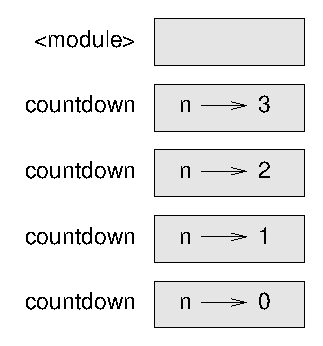
\includegraphics[scale=0.8]{figs/stack2.eps}}
\caption{スタック図}
\label{fig.stack2}
\end{figure} \par
%
関数は呼ばれる度にPythonは関数フレームを生成する。
このフレームには関数内のローカル変数や仮引数が含まれる。
再帰関数の場合には、同時にスタック上にある関数は一つ以上であるかもしれない。\par
図\ref{fig.stack2}は{\tt n=3}で呼ばれた{\tt countdown}関数のスタック図である。
いつものようにスタックの最上段は{\verb"__main__"}のフレームである。
このフレームは{\verb"__main__"}で生成された変数や引数が不明なので、空白である。
四つ{\tt countdown}フレームは仮引数の{\tt n}の値が異なっている。
スタックの底は{\tt n=0}のフレームで{\bf 基底ケース（base case）}と呼ばれている。
これは再帰的な呼び出しをしないのでこれ以上のフレームは存在しない。\par
練習問題として、{\tt print\_n}関数が {\tt s = 'Hello'}、{\tt n=2}で呼ばれたときのスタック図を描いてみよう。また
仮引数として関数オブジェクトと一つの数{\tt n}を仮引数とする再帰関数{\tt do\_n}を作成せよ。
この関数は問題の関数を{\tt n}回実行する。
%
\section{無制限な再帰}
もしある再帰処理が基底ケースを持たないとすると、再帰的な呼び出しは永遠に続くことになる。
これは{\bf 無制限な再帰（infinite recursion）}として知られていて、
一般に健康なアイデアではない。以下はその最小なプログラムの例である：
\begin{verbatim}
def recures():
    recures()
\end{verbatim}
大抵の開発環境では、このような無制限な再帰を含むプログラムは永遠に実行されることはない。
Pythonは再帰の深さの限界値に達するとエラーメッセージを吐き出す：
\begin{verbatim}
  File "<stdin>", line 2, in recurse
  File "<stdin>", line 2, in recurse
  File "<stdin>", line 2, in recurse
                  .   
                  .
                  .
  File "<stdin>", line 2, in recurse
RuntimeError: Maximum recursion depth exceeded
\end{verbatim}
このトレースバックは前章でみたものより長めである。このエラー発生時には、スタックには1000個の{\tt recures}フレームができる。
%
\section{キーボード入力}
これまで生成したプログラムはユーザからの入力を受け付ける機能がなく、いつも同じ動きをするもであった。\par
Pythonはキーボードから入力を受け付ける{\tt input}という組み込み関数を提供している。
Python2では{\tt raw\_input}だ。
この関数が呼ばれると、実行は停止し、ユーザからの入力待ちになる。
ユーザは{\tt Return}キーや{\tt Enter}キーを入力すると、
プログラムは再実行され、{\tt input}関数はユーザが入力したものを文字列として戻す。つまり、
\begin{verbatim}
>>> text = input()
What are you waiting for?
>>> text
'What are you waiting for?'
\end{verbatim}
ユーザからの入力を得る前に、ユーザに何を入力すべきか知らせることが賢明である。
関数{\tt input}は入力促進文字列を引数として受け取ることができる。つまり、
\begin{verbatim}
>>> name = input('What...is your name?\n')
What...is your name?
Arthur, King of the Britons!
>>> name
'Arthur, King of the Britons!'
\end{verbatim}
入力促進文字列の最後にあるシークェンス\verb"\n"は{\bf 改行（new line）}の記号で
これで改行が起きる。だから、入力文字はこの入力促進文字列の下に現れる訳である。\par
ユーザが整数値を入力すると期待できるときにはその戻り値を整数型に変換するとよい：
\begin{verbatim}
>>> prompt = 'What...is the airspeed velocity of an unladen swallow?\n'
>>> speed = input(prompt)
What...is the airspeed velocity of an unladen swallow?
42
>>> int(speed)
42
\end{verbatim}
しかし、ユーザが数字以外のものを入力しようとするとエラーが出る：
\begin{verbatim}
>>> speed = input(prompt)
What...is the airspeed velocity of an unladen swallow?
What do you mean, an African or a European swallow?
>>> int(speed)
ValueError: invalid literal for int() with base 10
\end{verbatim}
この種のエラーを処理する方法は後に学ぶ。
%
\section{デバッギング}
　エラーが発生したとき表示されるPythonのトレースバックは多くの情報を含んでいる。
しかし、スタック上のフレームが多数あるときには、その量の多さに圧倒される。その中で有用な情報は
\begin{itemize}
\item どのようなエラーか
\item どこで起きたか
\end{itemize}
構文エラーの場所を特定するのは一般的に易しいが、意外なものもある。空白やタブは見えないし無視しがちなので、空白によるエラーは陥りやすい：
\begin{verbatim}
>>> x = 5
>>>  y = 6
  File "<stdin>", line 1
    y = 6
    ^
IndentationError: unexpected indent
\end{verbatim}
この例では第二行が一つの空白でインデントされているのが問題である。
しかし、エラーメッセージは{\tt y}を指していて、誤解を生む可能性がある。\par
一般にエラーメッセージは問題が発生を確認した場所を示すが、
実際のエラーはそれ以前に原因があることもあり得る。ある場合では前の行にそれがある。\par
実行時エラーでも同様だ。あなたは信号・雑音比をデシベルで計算しようしているとしよう。式は \par
  $SNR_{db} = 10 \log_{10} (P_{signal} / P_{noise})$ \par
と書ける。これをPythonで書こうとすると以下のようになる：
\begin{verbatim}
import math
signal_power = 9
noise_power = 10
ratio = signal_power // noise_power
decibels = 10 * math.log10(ratio)
print(decibels)
\end{verbatim}
実行してみるとエラーメッセージに出会う：
\begin{verbatim}
Traceback (most recent call last):
  File "snr.py", line 5, in ?
    decibels = 10 * math.log10(ratio)
ValueError: math domain error
\end{verbatim}
このエラーメッセージは５行目を指しているが、ここにはおかしなところがない。
変数{\tt ratio}を{\tt print}してみることは助けになるかもしれない。
結果は{\tt }0である。つまり、問題は4行目にある。普通の除算の替わりに打ち切り除算が使われていることによる。
問題の解決は浮動小数点で計算すればよい。つまり普通の除算にすればよい。\par
一般にエラーメッセージは問題をどこで発見したかをわれわれに告げる。しかし、多くの場合そこはエラーの原因になる場所ではない。
（訳注：エラーメッセージにも注意する必要がある。この例では{\tt domain error}となっている。つまり関数の適用範囲を超えて
いることからくるエラーである。）　
%
\section{語句}
\begin{description}

\item[打ち切り除算（Floor division）：] 二つの数値の除算で結果の小数点以下を負の無限大の方向に丸める演算(例：{\verb"5//3 -> 1、-5//3->-2"}）。
\index{floor division}

\item[モジュラ演算子（modulus operator）：]一つの整数をもう一つの整数で割ったときの余りを生成する演算子でパーセント記号、（{\verb"%"}）が用いられる。.
%\index{modulus operator}
%\index{operator!modulus}

\item[ブール代数表現（boolean expression）：]その値が 「真」（{\tt True}）か「偽」（{\tt False}）になるような表式。.
%\index{boolean expression}
%\index{expression!boolean}

\item[比較演算子（relational operators）：]二つの被演算子を比較し、「真」、「偽」の値を返す演算子。 
{\tt ==}、{\tt !=}、{\tt >}、{\tt <}、{\tt >=},そして {\tt <=}がある。.

\item[論理演算子（logical operators）：]ブール代数表現を結合させるための演算子。{\tt and},、{\tt or}として{\tt not}がある。.

\item[条件文（conditional statement）：]ある条件に従って実行の流れを制御するための文。  
%\index{conditional statement}
%\index{statement!conditional}

\item[条件（condition）：]どちらの分岐を実行するか決めるための条件文の中で使われるブール代数表現。 
%\index{condition}

\item[複合文（compound statements）：]一つのヘッダーと一つのボディから構成される文。ヘッダーはコロン（\tt :）で終わり、
ボディはヘッダーの対してインデントされる。
%index{compound statement}

\item[分岐処理（branches）：]条件文の中で二者択一的に実行される文の一方。
%index{branch}

\item[条件文の連鎖（chained conditional）：] 二者択一の条件文を{\tt elif}文を使って連鎖させる。
%\index{chained conditional}
%\index{conditional!chained}

\item[入れ子の条件処理（nested conditionals）：]条件文の分岐処理の中で条件文を使う。  
%\index{nested conditional}
%\index{conditional!nested}

\item[再帰処理（recursion）：]実行中の関数のなかでその関数を呼ぶ処理。 
%\index{recursion}

\item[基底ケース（base case）：]再帰関数の中でその関数を再帰的に呼ばない分岐処理。
%\index{base case}

\item[無制限な再帰（infinite recursion）：]基底ケースを持たないまたはこれに達することがない再帰処理。最終的には無制限な再帰は実行エラーとなる。
%\index{infinite recursion}
\end{description}
%
\section{練習問題}

\noindent
{\bf 練習問題\tp.1} {\tt time}モジュールは同じ名前の{\tt time}関数を提供している。この関数は今のグリニッジ平均時間を
基点とした時間からの経過時間として戻す。{\tt UNIX}ではこの基点は1970年1月1日である。
\begin{verbatim}
>>> import time
>>> time.time()
1437746094.5735958
\end{verbatim}
この時間を読み込み、それを一日の時、分、秒に変換し、
且つ基点から何日経過したかを表示するスクリプトを作成せよ。\\

\noindent
{\bf 練習問題\tp.2}フェルマーの最後の定理は以下のような代数式を満たす整数$a$,$b$,$c$は存在しないと言う： \\
 \[ a^n + b^n = c^n \]　\\
ここで$n$は2より大きな任意の整数である。
\begin{enumerate}
\item 四つ仮引数{\tt a,b,c,n}を持つ関数{\tt check\_fermat}を作成せよ。この関数は{\tt n}が2より大きくしかも
 \[a^n + b^n = c^n \]
が成立したら、「おやまあ、フェルマーは間違っている」と表示し、さもないと「だめだ。成り立たない」と表示する。
\item ユーザにたいして整数{\tt a,b,c,n}の入力請求をして、これらを整数に変換し、
関数{\tt check\_fermat}でこれらの整数値がフェルマーの定理を満たさないかどうかを示す関数を作成せよ。
\end{enumerate}

\noindent
{\bf 練習問題\tp.3}三つの楊枝を使って三角形を作ることを試みる。
例えば、一つが12インチの楊枝で、他の二つは1インチの楊枝だとしよう。
これでは明らかに端と端を接して三角形を作ることはできない。
三つの任意の値に対して、三角形をつくる条件を調べることができる。 \par
三角形の一つの辺の長さが他の二辺の長さの和より大きいとこれでは三角形は作れない。
これ以外であれば作れる（二つの辺の長さは他の一辺に等しいときは、「縮退」三角形という）
\begin{enumerate}
\item 三つ整数を引数とする関数{\tt is\_triangle}を作成せよ。
この関数ではこれらの長さの楊枝から三角形が作れるときは{\tt "yes"}を{\tt print}し、それ以外は{\tt "no"}を{\tt print}する。
\item ユーザに三つの楊枝の長さを入力させ、関数{\tt is\_triangle}で検定するプログラムを作成せよ。
\end{enumerate}

\noindent
{\bf 練習問題\tp.4} 以下のプログラムはどのような出力を表示するか？結果を表示したときのスタック図を作成せよ。
\begin{verbatim}
def recurse(n, s):
    if n == 0:
        print(s)
    else:
        recurse(n-1, n+s)

recurse(3, 0)
\end{verbatim}
\begin{enumerate}
\item この関数を{\tt recurse(-1, 0)}で呼び出しと何が起こるか？
\item この関数を使うユーザのためにドキュメント文字列（過不足ないかたちで）を作成せよ。
\end{enumerate}

\noindent
以下の練習問題は第4章の{\tt turtle}モジュールを使う。 \\
{\bf 練習問題\tp.5}以下の関数を読みそれがどのようなことをしているか明らかにせよ。
そしてこれを実行してみよう（第4章の例を参照のこと）。
\begin{verbatim}
def draw(t, length, n):
    if n == 0:
        return
    angle = 50
    t.fd(length*n)
    t.lt(angle)
    draw(t, length, n-1)
    t.rt(2*angle)
    draw(t, length, n-1)
    t.lt(angle)
    t.bk(length*n)
\end{verbatim}
%
\begin{figure}[htbp]
\centerline
{
\includegraphics[scale=0.8]{figs/kochA.eps}}
\caption{コッホ曲線.}
\label{fig.koch}
\end{figure}

\noindent
{\bf 練習問題\tp.6}コッホ曲線は図\ref{fig.koch}のようなフラクタル図形である。長さ{$x$}の線分からコッホ曲線を描くには以下のような手順が必要になる：
\begin{enumerate}
\item $x/3$の長さでコッホ曲線を描く
\item 60度左転回
\item $x/3$の長さでコッホ曲線を描く
\item 120度右転回
\item $x/3$の長さでコッホ曲線を描く
\item 60度左転回
\item $x/3$の長さでコッホ曲線を描く
\end{enumerate}
例外は$x$が$3$よい小さいときで、長さ$x$の直線を描くことでよい。\\

\begin{enumerate}
\item {\tt turtle}と長さを仮引数とする関数{\tt koch}を作成せよ。この関数はこの与えられた長さでコッホ曲線を描く。
\item 関数{\tt snowflake}を三つのコッホ曲線から作成せよ。この関数は雪の微片の外周を表現する。\\
解答例：\url{https://thinkpython.com/code/koch.py}.
\item コッホ曲線はいろんな具合に一般化できる。\\
\url{http://en.wikipedia.org/wiki/Koch_snowflake}を参考にして自分の好みの図形を描くプログラムを作ってみよう。
\end{enumerate}
%
\chapter{結果を生む関数}
これまで使ってきた数学関数のようなPythonの関数の多くは戻り値を返すものである。
しかしこれまでに作成した関数は戻り値がない{\tt void}型であった。そ
れらはなにかを{\tt print}し、{\tt turtle}が動きまわる動作をしたが、戻り値が何もなかった。 \par
この章では結果を生む関数を書いてみることにする。
%
\section{戻り値}
このような関数を呼ぶと結果を返すので変数に代入するか、表式の一部として使う：
\begin{verbatim}
e = math.exp(1.0)
height = radius * math.sin(radians)
\end{verbatim}
これまでに作成した関数は戻り値がない{\tt void}型であった。
それら戻り値が何もないが、厳密に言うと{\tt None}という戻り値を持つ。 \par
第一の例は関数{\tt area}である。この関数は半径の値を引数として円の面積の値を戻す関数である：
\begin{verbatim}
def area(radius):
    a = math.pi * radius**2
    return a
\end{verbatim}
{\tt return}文については既に触れたが、結果を生む関数では、{\tt return}文には表式を付随する。
この文は、「この関数から直ちに戻り、以下の表式を返り値として使え」という意味だ。この表式は任意で、以下のように書くこともできる：
\begin{verbatim}
def area(radius):
    return math.pi * radius**2
\end{verbatim}
しかし、{\tt a}のような{\bf 一時変数（temporary variables）}の導入はデバッグを容易にしてくれることがある。\par
ときとして、多重の{\tt return}文の使用が有益なことがある。とくに条件文による分枝がある場合には、以下のようになる：
\begin{verbatim}
def absolute_value(x):
    if x < 0:
        return -x
    else:
        return x
\end{verbatim}
これらの{\tt return}文は二者択一なので、{\tt return}文はどちらかが実行される。 \par　
関数で{\tt return}文が実行されると、関数は他の文を実行せず、直ちに関数の動作は終了する。
このように{\tt return}文より後に置いた文や決して実行の流れが到達しないところにあるコードは{\bf 死コード（dead code）}と言われる。\par
結果を生む関数ではプログラムで想定される全ての可能な経路が必ずreturn文に到達することを確認する必要がある：
\begin{verbatim}
def abusolute_value(x):
    if x < 0:
        return x
    if x > 0:
        return x
\end{verbatim}
この関数は正しくない。{\tt x}の値がたまたま{\tt 0}であると、この関数は{\tt return}文に到達できない。
関数の実行は関数の終わりにある{\tt return}文で戻ることになる。この戻り値は{\bf ノン（None）}であり、{\tt 0}ではない。つまり
\begin{verbatim}
>>>print(absolute_value(0))
None
\end{verbatim} \par
Pythonは組み込み関数として絶対値を計算する{\tt abs}関数を提供している。\\
練習問題として比較関数を作成せよ。
つまり二つの引数{\tt x}と{\tt y}を持ち、
もしも{\tt x > y}ならば戻り値は{\tt 1}、{\tt x == y}ならば、{\tt 0}、{\tt x < y}ならば、{\tt -1}を返す関数である。
%
\section{段階的な改良法}
大きな関数を書き始めると、多分にデバッグに多くの時間を使うことになる。このような複雑なプログラムに取りかかると{\bf 段階的な改良法（incremental development）}と呼ばれている方法を取りたくなるだろう。この方法の目標は一時に追加・検証するコードを小刻みにし、膨大なデバッギングを避けることにある。\par
例をあげてみよう。与えられた二点 と からこの二点間の距離を求める問題だ。ピタゴラスの定理から
 \begin{displaymath}
\mathrm{distance} = \sqrt{(x_2 - x_1)^2 + (y_2 - y_1)^2}
\end{displaymath}
第一ステップはこの関数{\tt distance}はPythonではどんな形になるかなと考察することである。換言すれば、入力（仮引数）は何で、出力（戻り値）は何か？\par
この例では入力は二つ点、つまり四つの数値であり、戻り値は計算された距離になるであろうから浮動小数点数の値である。\par
ここまで分かると関数の骨格が書ける：
\begin{verbatim}
def distance(x1, y1, x2, y2):
    return 0.0
\end{verbatim}
この版では戻り値は常に{\tt 0}なので距離の計算はしていない。
しかし、この関数は構文的には正しく、ちゃんと動く。もつと複雑に関数を仕上げる前に関数の検証としてこれは使える。 \par
適当な引数を入れて検証する：
\begin{verbatim}
>>>distance(1, 2, 4, 6)
0.0
\end{verbatim}
水平方向の距離が{\tt 3}、垂直方向の距離が{\tt 4}の二点をわざわざ選んだ。
これには理由があり二点間の距離は{\tt }5となり、事前に答えが分かり関数の動作検証に都合がよいからだ。\par
この時点で関数{\tt distance}は構文的には問題ないことが確認できた。
次ぎにくる作業は関数のボディを書くことである。これにはこの二点の{\tt ｘ}方向の差、{\tt x2-x1}、{\tt ｙ}方向の差、{\tt y2-y1}を表示してみることだろう：
\begin{verbatim}
def distance(x1, y1, x2, y2):
    dx = x2 - x1
    dy = y2 - y1
    print('dx is',dx)
    print('dy is',dy)
    return 0.0
\end{verbatim}
この関数を実行してみると、``dx is 3"、``dy is 4"と表示されるはずだ。\par
次ぎのステップは{\tt dx}と{\tt dy}の二乗の和を求めることになる：
\begin{verbatim}
def distance(x1, y1, x2, y2):
    dx = x2 - x1
    dy = y2 - y1
    dsquared = dx**2 + dy**2
    print('dsquared is: ',dquared)
    return 0.0
\end{verbatim}
ここでまたこれを実行して出力を調べる。最後は平方根を計算する関数{\tt math.sqrt}を使いその結果を{\tt return}文で返す：
\begin{verbatim}
def distance(x1, y1, x2, y2):
    dx = x2 - x1
    dy = y2 - y1
    dsquared = dx**2 + dy**2
    result = math.sqrt(dsquared)
    return result
\end{verbatim}
これがうまく動くことが確認できれば完了である。そうでなければ、変数r{\tt esult}を{\tt return}文の前で表示してみるとよい。\par
この最終版の関数自体は何も表示しない。{\tt print}文の挿入はデバッギングに有効だ。
デバッグが終わったらこの{\tt print}文は削除する。
このようなコードは{\bf 足場組み（scaffolding）}と呼ばれる。
というのは、これらの{\tt print}文はプログラムを完成させることに有効だが、最終に生成されたものには含ませないからだ。 \par
プログラミングを始めた最初のころは一度に追加するのは１～２行にしておくとよい。
慣れてきたら、それより大きなまとまりを一度に書き、デバッグすることができるようになるはずだ。
いずれにせよ、この段階的な改良法は時間の節約になる。\par
このプロセスの特徴を箇条書きにすると以下のようになる：
\begin{enumerate}
\item 実行可能な小さなプログラムから始めて、少しずつ段階的に変更を加える。
いつの段階でもエラーが発生したら原因を突き止め修正しておく。
\item 一時変数を使い途中の値を保存し、それを必要に応じて表示、検証できるようにする。
\item 最終的なプログラムがうまく動くようになったら、足場の撤去やプログラムが読み難くならない範囲で、
複数の文を一つの複合表式に置き換えなどの作業をする。
\end{enumerate}
練習問題として直角三角形の二辺の長さを引数として受け取り、
斜辺の長さを戻り値として返す関数{\tt hypotenuse}を段階的な改良法を使って書け。各段階の状況を記録して置くこと。
%
\section{合成関数}
さて、これまでの議論で関数の中で別な関数を呼ぶことも可能だということを予想できたと思う。このような機能を{\bf 複合関数（composition）}という。\par
このような例として、円の中心の座標と円周上の座標の二点の座標を引数としてその円の面積を計算する関数を書いてみよう。\par
変数{\tt xc}、{\tt yc}に円の中心の座標の値が保存され、
{\tt xp}、{\tt xp}に円周上の座標の値が保存されているとしよう。
第一にすべきはこの二点を使って円の半径（{\tt radius}）を出すことである。これには関数{\tt distance}を使う：
\begin{verbatim}
radius = distance(xc, yc, xp, yp)
\end{verbatim}
次はこの半径から面積を出す関数{\tt area}を使う。ここでは形式的にのみ書いて置く：
\begin{verbatim}
result = area(radius)
\end{verbatim}
これらを一纏めにして一つの関数とする：
\begin{verbatim}
def circle_area(xc, yc, xp, yp):
    radius = distance(xc, yc, xp, yp)
    result = area(radius)
    return result
\end{verbatim}
{\tt radius}や{\tt result}の一時変数はプログラムの開発途上やデバッグには有効であるが、
最終的なプログラムでは関数を入れ子にして簡潔に書くこともできる：
\begin{verbatim}
def circle_area(xc, yc, xp, yp):
    return area(distance(xc, yc, xp, yp))
\end{verbatim}
%
\section{ブール代数関数}
ブーリアン（真理値）を返す関数は関数内部で複雑な検証を隠す上で有効なものである。例を上げる：
\begin{verbatim}
def is_divisible(x, y)
    if x % y == 0:
        return True
    else:
        return False
\end{verbatim}
ブール代数関数には二者択一のような関数名がよく付けられる。
関数{\tt is\_divisible}は{\tt x}が{\tt y}で割り切れるかどうかの結果を{\tt True}や{\tt False}として返す関数である。\\
実行例：
\begin{verbatim}
>>> is_divisible(6, 4)
False
>>> is_divisible(6, 3)
True
\end{verbatim} \par
比較演算子の結果の値がブーリアンなので関数は以下のように書ける：
\begin{verbatim}
def is_divisible(x, y):
    return x % y == 0
\end{verbatim} \par
ブール代数関数はよく条件文の中で使われる：
\begin{verbatim}
if is_divisible(x, y):
    print('x is divisible by y')
\end{verbatim}
もしかしたら以下のように書くかもしれない：
\begin{verbatim}
if is_divisible(x, y)==0:
    print('x is divisible by y')
\end{verbatim}
しかし、この比較は不必要である。\par
練習問題として以下のような関数{\tt is\_between(x, y, z)}を書け。
この関数は$x \le y \le z$ なら{\tt True}を返し、これ以外ならば{\tt False}を返す。
%
\section{再帰関数の拡張}
これまでの学習はPythonの一部分であるが、これまでの学習で得たもので完全なプログラミング言語になっていることを確認することは興味深いことであろう。
この完全という意味は計算したいと思われる全てのことがこの言語で書けるということである。
あなたがこれまで作成した如何なるプログラムもこれまで学習したPythonを使って書き換えることができる
（多分、キーボード、マウス、ディスクといった装置を制御するコマンドは別途必要かもしれない）。\par
この主張の証明はアラン・チューリングによって初めて自明なことではない課題であることが証明された。
かれは当時のコンピュータ科学者がそうであったように数学者であったが、コンピュータ科学者の嚆矢の一人である。
従って、この主張はチューリング・テストと言われている。このチューリング定理のもっと完全で（従って厳密な）議論は
``Introduction to the Theory of Computation"(Michael Sipser著)を参照してほしい。 \par
ここでは、これまで学習したツールを使って何ができるかの認識を得るために、再帰関数のいくつかを検討することにする。
再帰的定義は循環的定義に似ている。それらの定義にはそこでは定義するべきものの参照を含んでいる。\par
循環的定義はあまり有用ではない。たとえばこうだ：\par
\begin{quote}
{\tt vorpal}:何か{\tt vorpal}であるものを記述する形容詞である。
\end{quote}
こんな定義を辞書でみつけたらまごついてしまうかもしれない。\par
しかし、階乗関数が記号！で記述されているのを探し出したときには、その記述は以下のようなものだろう：
\begin{eqnarray*}
&&  0! = 1 \\
&&  n! = n (n-1)!
\end{eqnarray*}
この定義は{\tt 0}の階乗は{\tt 1}、その他の任意の値、{\tt n}の階乗は{\tt n-1}の階乗に{\tt n}を乗じたものであることを意味する。
だから{\tt 3!}は{\tt 3}掛け{\tt 2!}で、{\tt 2!}は{\tt 2}掛け{\tt 1!}で、{\tt 1!}は{\tt １}掛け0!である。
これを纏めると{\tt 3!}は$3\times 2\times 1\times 1$で{\tt 6}となる。\par
何かを再帰的な定義で記述できたならば、それをPythonでプログラムして評価することができる。\par
第一にすべきは、関数名とその仮引数を決めることである。今回の場合、その関数{\tt factorial}の仮引数は一つの整数である。つまり
\begin{verbatim}
def factorial(n):
\end{verbatim}
となる。この引数がたまたま{\tt 0}であると、この関数の返すべき値は{\tt 1}であるので
\begin{verbatim}
def factorial(n):
    if n == 0:
        return 1
\end{verbatim}
となる。さもないと、これが興味あるケースであるが、再帰呼び出しで{\tt n-1}の階乗を求め、
それに{\tt n}を乗ずる計算をすることになる。従って、プログラムは以下の様になる：
\begin{verbatim}
def factorial(n):
    if n == 0:
        return 1
else:
    recurse = factorial(n-1)
    result = n * recurse
    return result
\end{verbatim}
このプログラムの実行の流れは\ref{recursion}節で登場した{\tt countdown}と似たものになる。nの値を3にしてこの関数を呼んだときの流れを以下に示す：
\begin{verbatim}
3は0でないので、第二の分枝をとり、n-1の階乗を計算する。
　　2は0でないので、第二の分枝をとり、n-1の階乗を計算する。
　　　　1は0でないので、第二の分枝をとり、n-1の階乗を計算する。
　　　　　　0は0であるので、第一の分枝をとり、単に1を戻り値として返す。
　　　　戻り値1をrecurseに代入、これとn（即ち1）とを乗じた値1を返す。
　　戻り値1をrecurseに代入、これとn（即ち2）とを乗じた値2を返す。
戻り値2をrecurseに代入、これとn（即ち3）とを乗じた値6を返す。
\end{verbatim}
これでこの関数を最初に呼んだ関数に戻る。\par
図\ref{fig.stack3}にこの関数呼び出しのスタック図を示した。戻り値はスタック図を繋ぐ経路に添付した。
各フレームでは戻り値はそのフレームの{\tt result}が持っている値である。
最後のフレームでは流れは{\tt if}文の第一分枝になるので、ローカル変数{\tt recures}と{\tt result}は存在しない。
%
\begin{figure}[htbp]
\centerline
{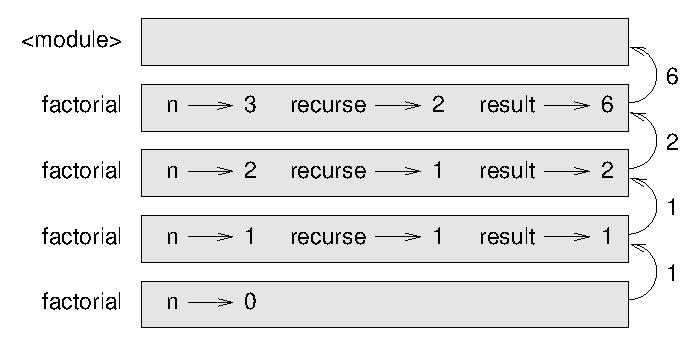
\includegraphics[scale=0.8]{figs/stack3.eps}}
\caption{スタック図.}
\label{fig.stack3}
\end{figure}
%
\section{信用して跳び越える}
実行の流れを追うことはプログラムを読むひとつの方法であるが、直ぐに複雑になる。
別な方法は私が「信用して跳び越える」と呼ぶ方法である。
関数に出会ったらその関数内の流れを追跡するかわりに、その関数は正常に動作し、
正しい戻り値を返すとみなし、この関数内の実行の流れをスキップする。\par
このようなスキップは既に組み込み関数では経験している。
{\tt math.exp}や{\tt math.cos}の関数ではこれらの関数内の流れには頓着しない。
われわれはこれらの関数は優秀なプログラマーが作成したもので、正常に動作するとみなしている。\par
同じことが自作関数でもいえる。例えば、6.4節で作成した{\tt divisible}関数だ。
コードの吟味や検証で正常に動作することが確証できたら、
以後はこのボディの実行の流れには頓着しない。 \par
同じことが再帰関数でもいえる。再帰関数の呼び出しに出会ったら、
その関数内の流れを追わず、その再帰的な呼び出しは正常に動作する（正しい戻り値を返す）とみなす。
そして、「もし{\tt n-1}の階乗が計算できたら、それで{\tt n}の階乗が計算できるか？」と自問してみる。
この場合、{\tt n-1}の階乗に{\tt n}を乗ずれば答えになることは明らかである。 \par
勿論、まだ書き上げてもいない関数が正常に動作するとみなすことは少々奇妙であるが、
これは「信用して跳び越える」という言葉の所以である。
%
\section{もう１つの例題}
関数{\tt factorial}に引き続き数学的な再帰関数として引き合いに出される{\tt fibonacci}関数である。
この関数の定義は以下のようである：
\begin{eqnarray*}
&& \mathrm{fibonacci}(0) = 0 \\
&& \mathrm{fibonacci}(1) = 1 \\
&& \mathrm{fibonacci}(n) = \mathrm{fibonacci}(n-1) + \mathrm{fibonacci}(n-2)
\end{eqnarray*}
（\url{http://en.wikipedia.org/wiki/Fibonacci_number}も参照のこと） \par
これをPythonに翻訳するとこんな風になる：
\begin{verbatim}
def fibonacci(n):
    if n == 0:
        return 0
    elif n == 1:
        return 1
    else:
        return fibonacci(n-1) + fibonacci(n-2)
\end{verbatim}
この関数の実行の流れをまともに追跡すると、{\tt n}が小さい場合でさえ頭が爆発してしまう。
しかし、「信用して跳び越える」方法に従って、二つ再帰呼び出しは正常に実行されると仮定すると、
第三分枝の計算で正しい答えが戻ることは自明となる。
%
\section{型の検証}
関数{\tt factorial}を引数の値に{\tt 1.5}を入れて呼ぶとどうなるだろうか？
\begin{verbatim}
>>>factorial(1.5)
RuntimeError: maximum recursion depth exceeded 
\end{verbatim}
この実行時のエラーは制限なしの再帰に起因するようにみえる。どうしてそんなことが起きるのか？
この関数には基底ケースが考慮されているではないか。
引数{\tt n}が整数でないと、この基底ケースをすり抜けてしまい、制限なしの再帰になるのだ。\par
上の引数では、最初の再帰で引数nの値は{\tt 0.5}になり、二回目は{\tt -0.5}となる。
だから基底ケースである{\tt n=0}は実現しない。\par
対策としては二つの方向がある。一つは{\tt factorial}を拡張して引数は浮動小数点数にも対応できるようにする。
二つ目は引数型を検証するように書き改めることである。
第一はガンマ関数への拡張であり、この本の範囲を超えるので、第二番目の方法を紹介する。\par
引数の型を調べるために組み込み関数{\tt isinstance}を使う。
これと同時に引数が正の数であることも調べることにする。プログラムは以下のようになる：
\begin{verbatim}
def factorial(n):
    if not isinstance(n, int):
        print('Factorial is only defined for integers.')
        return None
    elif n < 0:
        print('Factorial is not defined for negative integers.')
        return None
    elif n == 0:
        return 1
    else:
        return n * factorial(n-1)
\end{verbatim}
第一番目の基底ケースは非整数対策であり、第二番目の基底ケースは負整数対策である。
どちらも何らかの問題があるというメッセージを吐き出し、戻り値は{\tt None}である：
\begin{verbatim}
>>> print(factorial('fred'))
Factorial is only defined for integers.
None
>>> print(factorial(-2))
Factorial is not defined for negative integers.
None
\end{verbatim}
この二つの検証を通過したら、引数{\tt n}は正か{\tt 0}の整数である。この状態になれば、
この再帰呼び出しは有限回で停止することが証明できる。\par
このプログラムはときとして{\bf 保護回路（guardian）}と呼ばれる手法を例示したことになる。
最初の二分枝は保護回路で実行時エラーを引き起こすだろうと思われる値からコードを保護する役目をしている。 \par
11.4節ではエラーの表示の替わりに例外処理を実行するもっと融通の効く手法に出会うはずだ。
%
\section{デバッギング}　
大きなプログラムをそれより小さい関数に分割することはそれ自体でデバッグの極自然な確認の単位になる。
もし関数が正常に動作しないとなると、考えなければならないことは以下の三点である：
\begin{itemize}
\item 関数の事前条件に違反するような引数の問題。
\item 関数の事後条件に違反する問題。
\item 関数の戻り値やそれの使われ方の問題。
\end{itemize}
最初の可能性を除外するには関数の先頭に{\tt print}文を挿入し、仮引数の値（そして型も）を表示してみるとよい。
または、関数のコード自体にこの機能を持たせるとよい。仮引数に問題がないとすると、
次は関数の{\tt return}文の前で戻り値を表示してみる。もし可能ならば、この戻り値を紙で計算してみる。
簡単な引数の値であれば、その関数の戻り値を手計算することは容易い（6.2節をみよ）。 \par
関数の最初と最後に{\tt print}文を追加・挿入することは実行の流れを可視化する上で有用である。
以下は{\tt factorial}に{\tt print}文を追加したものである：
\begin{verbatim}
def factorial(n):
    space = ' ' * (4 * n)
    print(space, 'factorial', n)
    if n == 0:
        print(space, 'returning 1')
        return 1
    else:
        recurse = factorial(n-1)
        result = n * recurse
        print(space, 'returning', result)
        return result
\end{verbatim}
変数{\tt space}は出力のインデントを制御する空白文字列である。{\tt factorial(5)}の結果を示す：
\begin{verbatim}
                     factorial 5
                 factorial 4
             factorial 3
         factorial 2
     factorial 1
 factorial 0
 returning 1
     returning 1
         returning 2
             returning 6
                 returning 24
                     returning 120
\end{verbatim}
実行の流れについて混乱してしまったときは、このような出力は有用になる。
このような効果的な足場を据えることには時間が掛かるが、ちょっとした足場もデバッギングの時間を節約することができる。
%
\section{語句}
\begin{description}
\item[一時変数（temporary variables）：]複雑な計算の際に中間結果を保存する目的で使われる変数。
%\index{temporary variable}
%\index{variable!temporary}

\item[死コード（dead code）：]如何なるばあいでも到達しないプログラムの部分。{\tt return}文の後にあることが多い。  
%\index{dead code}

\item[段階的な改良法（incremental development）：]一時に少量の追加とテストを行いつつプログラムを開発する手法。
%\index{incremental development}

\item[足場組み（scaffolding）：]最終版では削除されるがプログラム開発の途上で使われるコード。
%\index{scaffolding}

\item[保護回路（guardian）：]エラーを引き起こす状況を検出及び回避するために条件文を使うプログラムの部分。
%\index{guardian pattern}
%\index{pattern!guardian}
\end{description}
%
\section{練習問題}
\noindent
{\bf 練習問題\tp.1} 以下のようなプログラムのスタック図を示せ。さらに実行したとき、如何なる表示が出るか答えよ。
\begin{verbatim}
def b(z):
    prod = a(z, z)
    print(z, prod)
    return prod

def a(x, y):
    x = x + 1
    return x * y

def c(x, y, z):
    total = x + y + z
    square = b(total)**2
    return square

x = 1
y = x + 1
print(c(x, y+3, x+y))
\end{verbatim}

\noindent
{\bf 練習問題\tp.2} {\tt Ackermann}関数は以下のように定義される：\\
%\begin{eqnarray*}
%A(m, n) = \begin{cases} 
%             n+1 & \mbox{if } m = 0 \\ 
%        A(m-1, 1) & \mbox{if } m > 0 \mbox{ and } n = 0 \\ 
%A(m-1, A(m, n-1)) & \mbox{if } m > 0 \mbox{ and } n > 0.
%\end{cases} 
%\end{eqnarray*}
%

$
A(m, n) = \left\{\begin{array}{ll}
             n+1 & \mbox{if } m = 0 \\ 
        A(m-1, 1) & \mbox{if } m > 0 \mbox{ and } n = 0 \\ 
A(m-1, A(m, n-1)) & \mbox{if } m > 0 \mbox{ and } n > 0.
\end{array}\right\}
$
\\

\noindent
（この関数については、 \url{http://en.wikipedia.org/wiki/Ackermann_function}.を参照のこと。）
{\tt Ackermann}関数の値を計算する関数{\tt ack}を作成せよ。
そして、{\tt ack(3, 4)}の値{\tt 125}を調べよ。大きな{\tt m}や{\tt n}では何が起こるか調べよ。\\
解答例：\url{https://thinkpython.com/code/ackermann.py} \\

\noindent
{\bf 練習問題\tp.3}回文とは、例えば``noon"や``redivider"のように後から読んでも、
前から読んでも同じ綴りを持つ言葉である。
再帰的には、もしある言葉の最初と最後の文字が同じで、
残った中間の文字列が回文であるなら、この言葉は回文である。\par
次ぎのような文字列処理の関数はその文字列の最初の文字、最後の文字、中間の文字列を戻り値とする：
\begin{verbatim}
def first(word):
    return word[0]

def last(word):
    return word[-1]

def middle(word):
    return word[1:-1]
\end{verbatim}
これらの関数の詳細は第8章で議論することになる。
\begin{itemize}
\item これらの関数を{\tt palindrome.py}と名付けたファイルとして生成せよ。
関数{\tt middle}に二文字の言葉を入れると戻り値はどうなるか？
一文字ではどうか？一文字も含まない文字列、つまり''ではどうか？
\item 引数として文字列を受け取る関数{\tt is\_ palindrome.py}を作れ。
この関数の戻り値はこの文字列が回文であると{\tt True}、さもないと{\tt False}である。
文字列の長さは関数{\tt len}で調べられることに注意。
\end{itemize} 
解答例：\url{https://thinkpython.com/code/palindrome_soln.py}. \\

\noindent
{\bf 練習問題\tp.4}一つの数{\tt a}は、もしもこの数が{\tt b}で割り切れ、
しかも{\tt a/b}が{\tt ｂ}のべき乗であるとき、{\tt b}のべき乗である。\par
二つの仮引数{\tt a}、{\tt b}を持つ関数i{\tt s\_power}を作成せよ。
この関数は{\tt a}が{\tt b}のべき乗であるときに{\tt True}を返す。 \\
注）基底ケースについて考慮せよ。\\

\noindent
{\bf 練習問題\tp.5}二つ整数{\tt a}、{\tt ｂ}の最大公約数（GCD）はこの二つの整数を除算して余りがない整数のなかで最も大きな整数である。\par
最大公約数を探す一つの方法はユーグリッド互除法である。この方法は{\tt a}を{\tt b}で割ったときの余りを{\tt r}とすると、$gcd(a,b) = gcd(b,r)$であることからきている。基底ケースは$gcd(a,0) = a$を使う。 \par
二つの整数{\tt a}、{\tt b}を仮引数とする関数{\tt gcd}を作成せよ。戻り値はこの二つの数の最大公約数である。\\
この練習問題の出典は、Abelson and Sussman,``Structure and Interpretation of Computer Programs"である。
%
\chapter{繰り返し処理}
この章では繰り返し処理について学ぶ。この種の繰り返し処理のお陰で文の集合を繰り返し実行できる。
既に\ref{recursion}節で再帰処理による繰り返しを見てきた。また4.2節では{\tt for}ループによるによる処理を
見てきた。この章では{\tt while}文によるもう一つの繰り返しをみよう。しかしその前に
代入について考察したい。

\section{多重代入}
これまで経験したことから分かるが、同じ変数に複数回の代入をすることは合法である。
この新しい代入で変数はこの新しい値を参照することになる（古い値の参照は停止する）。
\begin{verbatim}
>>> x = 5
>>> x
5
>>> x = 7
>>> x
7
\end{verbatim}
%
最初の{\tt x}を表示するとその値は{\tt 5}であったが、二回目ではその値は{\tt 7}となった。
図\ref{fig.assign2}には{\bf 多重代入（multiple assignment）}のスタック図の様子を示した。\par
%
\begin{figure}[htbp]
\centerline
{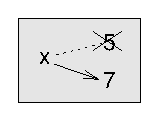
\includegraphics[scale=0.8]{figs/assign2.eps}}
\caption{状態図.}
\label{fig.assign2}
\end{figure}
%
多重代入で重要なことは代入処理と等値の違いを明確にしておくことだ。
Pythonでは等号（{\tt =}）は代入に使われるので、{\tt a=b}のような文を等値と解釈しがちである。これは間違いだ。
第一に、等値は左辺と右辺が対称だが、代入は対称でない。
例えば、数学的では、{$a=7$}と{$7=a$}は同じ意味だが、Pythonでは違う。
更に、数学では等値は常に真が偽の値を持つ。だから、もし{$a=b$}なら{$a$}と{$b$}とは常に等値である。Pythonの代入文でも二つの変数の値を同じにすることができるが、
常に同じ値を持つとは限らない。
\begin{verbatim}
>>> a = 5
>>> b = a #aとbとは同じ値を持つ
>>> a = 3 #aとbとは最早同じ値ではない
>>> b
5
\end{verbatim}
第三行目で{\tt a}の値が変わるが、{\tt b}の値は変わらない。だから、この二つは最早等しくはない。\par
多重代入は頻繁に使うが、注意が必要だ。変数の値が頻繁に変わるのでプログラムが読み辛いものになりがちでデバッグが難しくなる。
%
\section{変数更新}
最も頻繁に遭遇する多重代入は{\bf 変数更新（update）}である。新しい値が古い値に依存するかたちをとる：
\begin{verbatim}
x = x + 1
\end{verbatim}
この意味は、「{\tt x}の現在の値に{\tt 1}を加えてものを{\tt x}の新しい値として更新せよ」。 \par
存在しない変数の値の更新は、Pythonは代入の前に右辺を評価しなければならないので、エラーになる。
\begin{verbatim}
>>> x = x + 1
NameError: name 'x' is not defined
\end{verbatim}
変数の更新をする前に、変数は初期化（initialize）、一般に簡単な代入だが、しなければならない。
\begin{verbatim}
>>> x = 0
>>> x = x + 1
\end{verbatim}
変数の更新で{\tt 1}を加えて更新することを{\bf インクリメント（increment）}、
{\tt 1}を減じて更新することを{\bf デクリメント（decrement）}と特別な名称が付けられている。
%
\section{while文}
コンピュータは繰り返しを自動的に実行するタスクに頻繁に使われる。
同じか類似の処理を間違いなしで繰り返し実行するタスクはヒトでは苦手だが、コンピュータは得意としている。\par
これまで{\tt countdown}と{\tt print\_n}というプログラムをみてきた。
これらのプログラムは再帰を使っているが、{\bf 繰り返し処理（iteration）}の例だ。
繰り返し処理は頻繁に使うので、Pythonは言語仕様として豊富な繰り返し機能を提供している。
その一つが4.2節で紹介した{\tt for}文である。
これは後に議論する。\par
もう一つが{\tt while}文である。{\tt countdown}を{\tt while}で書いたものが以下である：
\begin{verbatim}
def countdown(n):
    while n > 0:
        print n
        n = n - 1
    print('Blastoff!')
\end{verbatim}
この{\tt while}文は英文を読むように読める。
つまり、「{\tt n}が{\tt 0}より大きい間、{\tt n}の値を表示し、
{\tt n}の値を{\tt 1}減じなさい。{\tt ｎ}が{\tt 0}になったとき単語{\tt Blastoff!}を表示しなさい」。\par
もう少し厳密に{\tt while}文の実行の流れを述べてみる：
\begin{itemize}
\item 条件を評価し、真か偽を得る。
\item 偽ならば、{\tt while}文のブロックを抜け、次ぎの文から実行を続ける。
\item 真ならば、{\tt whike}文のボディを実行して、最初に戻る。
\end{itemize}
この種の実行の流れを{\bf ループ（loop）}と称する。 \par
ループの本体の中で一つか二つの変数を更新し、ループの終了が保証されているようにしなければならない。
さもないとそのループは{\bf 無限ループ（infinte loop）}になる。
コンピュータ科学者にとって、「よく泡立て、よく洗い、これを繰り返す」というシャンプーの使用説明はひやかしの尽きない源である。\par
関数{\tt countdown}のばあいは{\tt n}の値が有限で、ループを繰り返す度に{\tt n}が減少するので、いずれは{\tt 0}になることが証明される。 \par
一般的にはこれは容易くない：
\begin{verbatim}
def sequence(n)
    while n != 1:
        print(n)
        if n%2 == 0:  #nは偶数
            n = n/2
        else:          #ｎは奇数
            n = n*3+1
\end{verbatim}
このループの条件は{\tt n != 1}、だからループは{\tt n}が{\tt 1}に達し、条件が偽になるまで続く。\par
毎回{\tt n}の値が表示され、{\tt n}が奇数か偶数かが検定される。
もし偶数であるとすると、{\tt n}は{\tt 2}で割られる。奇数であると、{\tt n}の値は{\tt n*3+1}に置き換わる。
例として{\tt 3}を引数としてこの関数が呼ばれると、表示は{\tt 3,10,5,16,8,4,2,1}となる。\par
{\tt n}はときとして増加、またときとして減少するので、このプログラムで{\tt n}が1に達し、
プログラムが終了することを証明するのは自明ではない。
例えば、{\tt n}が{\tt 2}のべき乗で出発すると{\tt n}は{\tt １}に達すまで偶数のままである。
前の例は{\tt 16}以降の系列はこのケースである。\par
如何なる正整数{\tt n}に対してもこのループが停止することを証明することは難しい問題だ。
これまで、これをできた人がいないし、できないということを証明できた人もいない。 \par
（参考：\url{http://en.wikipedia.org/wiki/Collatz_conjecture}） \par
練習問題として、関数{\tt print\_n}を再帰でなく、繰り返し処理をするプログラムに書き換えよ。
%
\section{ブレイク}
 ときとしてループの本体を実行している途中まで何時ループから抜け出るべきかを知ることができない場合がある。
このときは{\tt break}文でループを脱出する。 \par
例えば、{\tt done}とタイプされるまでユーザの入力を受け付けることを考えてみよう。プログラムは以下のようになる：
\begin{verbatim}
while True:
    line = input('> ')
    if line == 'done':
        break
    print(line)

print('Done!')
\end{verbatim}
ループの条件は常に真であるから、このループは{\tt break}に遭遇するまで続く。
その繰り返し毎にユーザ入力促進が一つのアングルブラケットで示される。
ユーザが{\tt done}と入力すると、{\tt break}文でループを抜ける。
そうでなければ、入力したものが何であってもそれを表示してループの先頭に戻る。
実行例：
\begin{verbatim}
> not done
not done
> done
Done!
\end{verbatim}
これはwhile文の使い方としては極普通である。
ループの検定はどこでもできるし（ループの先頭でなくても）、終了条件を否定的（これが起きるまで続く）でなく、
確定的（これを起きたとき終了）にも表現できる。
%
\section{平方根}
ループ処理は適当な答えから出発した数値計算でその答えを徐々に改良して行くときによく使われる。\par
例としてある数の平方根を求める手法としてニュートン法がある。
ある数$a$の平方根を知りたいとしよう。それに近い数$x$から出発して、以下の式を使うとさらによい近似値、yが得られる：
\[ y = \frac{x + a/x}{2} \]
 例として、{\tt a}が{\tt 4}で、{\tt x}が{\tt 3}のばあいと計算してみる：
 \begin{verbatim}
>>> a = 4
>>> x = 3
>>> y = (x + a/x) / 2
>>> y
2.16666666667
\end{verbatim}
この値はより真の値（$\sqrt{4} = 2$ ）に近い。この得られた新しい値を使ってプロセスを繰り返すともっと近い値が得られる：
\begin{verbatim}
>>> x = y
>>> y = (x + a/x) / 2
>>> y
2.00641025641
\end{verbatim}
これを数回繰り返すと推定値はほぼ正解になる：
\begin{verbatim}
>>> x = y
>>> y = (x + a/x) / 2
>>> y
2.00001024003
>>> x = y
>>> y = (x + a/x) / 2
>>> y
2.00000000003
\end{verbatim}
%
一般に真の値を得るには何回の繰り返しが必要なのかは事前には分からない。
しかし、推定値の表示が変動しなくなるところで、真の値の達したと考えてよい：
\begin{verbatim}
>>> x = y
>>> y = (x + a/x) / 2
>>> y
2.0
>>> x = y
>>> y = (x + a/x) / 2
>>> y
2.0
\end{verbatim}
%
つまり、{\tt y == x}で繰り返しを終了する。
纏めると、初期推定値{\tt x}から出発してそれが変化しなくなるまで繰り返すことにする：
\begin{verbatim}
while True:
    print(x)
    y = (x + a/x) / 2
    if y == x:
        break
    x = y
\end{verbatim} \par
この考えで大部分の{\tt a}についてはよさそうだ、しかし浮動小数点数の等値に関連する問題を含んでいる。
浮動小数点数は近似的に正しいのみである。
例えば、{$1/3$}のような有理数、$\sqrt{2}$のような無理数は浮動小数点数では正確には表現できない。\par
そこで、{\tt x}と{\tt y}が正確に一致するという替わりに、この２つの値の差の絶対値を計算し、
この差の絶対値に制限を置くことにする。ある値の絶対値は組み込み関数{\tt abs}を使う。
\begin{verbatim}
    if abs(y-x) < epsilon
        break
\end{verbatim}
ここで{\tt epsilon}は{\tt 0.0000001}のような数で、二つの値{\tt x},{\tt y}がどの程度近ければよいかを決める。
%
\section{アルゴリズム}
ニュートン法は{\bf アルゴリズム（algorithms）}の一例である。
それは機械的な方法である種の問題を解く方法のことである（いまの場合は、平方根を求める）。\par
アルゴリズムとは何かを定義することはそんなに易しくない。アルゴリズムでないものから議論したら理解が進むかもしれない。
一桁のかけ算を学んだ過程で、九九の表を暗記することになるはずだ。
この知識で特別な値を持った100個の場合のかけ算の解法が得られたことになる。しかし、このような知識はアルゴリズム的でない。 \par
もしあなたが「怠け者」で、このような暗記をなるべく減らしたいとして頭を使ったとしよう。
例えば、9桁の九九は{\tt n}を他の整数とすると、かけ算の答えは十の位は{\tt n-1}で、一の位は{\tt 10-n}であるとすればよいと発見したとしよう。
この発見は任意の整数nに対して成り立つ操作だ。このようなものがアルゴリズムである。 \par
同様に、加算での繰り上げ、減算の繰り下げの操作がアルゴリズムである。
アルゴリズムの一つの特徴はその操作に知性を必要としないことだ。
それらは最初から最後まで簡単な規則に沿って進められる機械的なプロセスである。\par
アルゴリズムの実行は退屈なものであるが、アルゴリズムを設計することは興味深く、知性的な挑戦であり、プログラミングの中枢である。\par
ヒトが何の苦もなく無意識にやっているいくつかのことをアルゴリズムとして定式化することは最も難しい。
自然言語はその卑近な例である。ヒトはそれをやっているが、これまでどのようにしてヒトがそれをやっているのか説明できないでいるし、
少なくともアルゴリズム的に定式化できないでいる。
%
\section{デバッギング}
大きなプログラムを書き始めると、デバッギングに掛ける時間が多くなる。
より大きなコードはより多くのエラーの機会があり、より多くの場所にバグが潜んでいることを意味する。\par
時間を短縮する一つの方法は、「二分割デバッグ法」とでもいう方法だ。例えば、100行あるコードを一時にチェックしようとすると100行をみる時間が必要になる。
そこで、プログラムを半分に分割する。手頃な半分あたりでよい。
そこに{\tt print}文（またはおなじ効果が得られるものでよい）を追加し、プログラムを実行してみる。
このチェックポイントまでで間違いが分かれば、前半に問題があることになるし、間違いがなければ、問題は後半にあることになる。\par
このように毎回二分割して行く。この操作を数回（これは100よりは少ない）すれば、理論的にはコードの１，２行に問題を絞り込むことができる。\par
実際には、「プログラムの半分」を見つけることが難しいことがあるが、行数を数えてまん中を見つけることは意味がない。
エラーが潜んでいそうな場所や、値をチェックするのに都合がよい場所の目星をつける。
そして、エラーがその前後で起きているらしいところをチェックポイントとして選べばよい。
%
\section{語句}
\begin{description}

\item[多重代入（multiple assignment）：]プログラムの実行の過程で一つの変数に一回以上の代入をすること。 
%\index{multiple assignment}
%\index{assignment!multiple}

\item[変数更新（update）：]変数の古い値に依存するかたちでその変数の値を更新する。 
%\index{update}

\item[初期化（initialize）：]変数更新をするつもりの変数に特定の値（初期値）を与える。
%\index{initialization!variable}

\item[インクリメント（increment）：] 変数の値を1だけ増加させる変数更新。
%\index{increment}

\item[デクリメント（decrement）：] 変数の値を1だけ減ずる変数更新。
%\index{decrement}

\item[繰り返し処理（iteration）：] 再帰呼び出しやループを使ってプログラムの一部を繰り返し実行する。
%\index{iteration}

\item[無限ループ（infinte loop）：] 終了条件が満たされることのないループ。
%\index{infinite loop}

\item[アルゴリズム（algorithms）：] 典型的な諸問題を解く一般的な手続き。
%\index{algorithm}

\end{description}

\section{練習問題}

\noindent
{\bf 練習問題\tp.1} 7.5節の繰り返し処理をコピーしてそれを{\tt mysqrt}と名前の関数としてカプセル化せよ。
この関数は{\tt a}を引数として持ち、{\tt x}の適当な値を設定し、戻り値として{\\ a}の平方根
の近似値を戻す。\par
この関数をテストするために{\tt test\_square\_root}というプログラムを作り、組み込み関数{\tt math.sqrt}の結果と
比較する以下のようなテーブルを作れ。
\begin{verbatim}
a   mysqrt(a)     math.sqrt(a)  diff
-   ---------     ------------  ----
1.0 1.0           1.0           0.0
2.0 1.41421356237 1.41421356237 2.22044604925e-16
3.0 1.73205080757 1.73205080757 0.0
4.0 2.0           2.0           0.0
5.0 2.2360679775  2.2360679775  0.0
6.0 2.44948974278 2.44948974278 0.0
7.0 2.64575131106 2.64575131106 0.0
8.0 2.82842712475 2.82842712475 4.4408920985e-16
9.0 3.0           3.0           0.0
\end{verbatim}
第一列は数値{\tt a}、第二列は7.5節で検討した関数で計算した平方根の値、
第三列は{\tt math.sqrt}で計算した値、第四列は二つの計算結果の差の絶対値である。 \\

\noindent
{\bf 練習問題\tp.2} 組み込み関数{\tt eval}は文字列を引数として受け取り、Pythonインタプリタでその文字列を評価する関数である。
例えば
\begin{verbatim}
>>> eval('1 + 2 * 3')
7
>>> import math
>>> eval('math.sqrt(5)')
2.2360679774997898
>>> eval('type(math.pi)')
<class 'float'>
\end{verbatim}
繰り返しユーザに入力請求をして文字列を入力、それを{\tt eval}で評価して結果を表示するプルグラム{\tt eval\_loop}を作成せよ。
この関数はユーザが{\tt 'done'}を入力したらループを抜け、最後に評価した値を戻り値とする。\\

\noindent
{\bf 練習問題\tp.3} 数学者Srinivasa Ramanujanは以下の公式が$1/\pi$の近似値を生成することを発見した：
 \[ \frac{1}{\pi} = \frac{2\sqrt{2}}{9801} 
\sum^\infty_{k=0} \frac{(4k)!(1103+26390k)}{(k!)^4 396^{4k}} \]
この公式を使い関数{\tt estimate\_pi}を作成せよ。
数列の項の和を求めるところに{\tt while}ループを使い、項が充分に小さくなったところ（$10^{-15}$）でそのループを抜ける。
結果を{\tt math.pi}と比較せよ。\\
解答例：\url{https://thinkpython.com/code/pi.py}.
%
\chapter{文字列}
文字列は整数、浮動小数点数、ブーリアンと異なっている。文字列は{\bf 配列（sequence）}である。その意味は
他の値を集めた順序だった集合である。この章では文字列を作っている個々の文字にアクセスする方法
についてみる。そして文字列に付随するメソッドの幾つかについて学ぶ。
%
\section{文字列は文字の配列}
文字列は配列である。角括弧で文字列の一つの文字にアクセスすることができる。
\begin{verbatim}
>>> fruit = 'banana'
>>> letter = fruit[1]
\end{verbatim}
第二の命令では文字列{\tt fruit}から一文字を選び、それを{\tt letter}に代入している。\par
角括弧の中の表式は{\bf インデックス（index）}と呼ばれている。このインデックスはどの文字を選びたいかを示すものである。 \par
しかし、結果はあなたが期待したものでないかもしれない：
\begin{verbatim}
>>> letter
a
\end{verbatim}
多くの人々にとっては、{\tt 'banana'}の最初の文字は{\tt b}であって{\tt a}ではない。
しかし、コンピュータ科学者にとっては、インデックスは文字列の最初の文字からのオフセット（片寄り）であり、最初の文字のオフセットは{\tt 0}である。
\begin{verbatim}
>>> letter = fruit[0]
>>> letter
b
\end{verbatim}
だから、{\tt b}は0番目の文字であり、{\tt a}は１番目の文字、{\tt n}は2番目の文字である。\par

このインデックスの表式は、変数や演算子を含めて任意である：
\begin{verbatim}
>>> i = 1
>>> fruit[i]
'a'
>>> fruit[i+1]
'n'
\end{verbatim}
しかしインデックスの値は整数でなければならない。さもないとエラーになる：
\begin{verbatim}
>>> letter = fruit[1.5]
TypeError: string indices must be integers, not float
\end{verbatim}
%
\section{{\tt len}}
組み込み関数{\tt len}は文字列の長さを返す関数である。
\begin{verbatim}
>>> fruit = 'banana'
>>> len(fruit)
6
\end{verbatim}
文字列の最後の文字を得ようとしたとき、以下のようにするかもしれない：
\begin{verbatim}
>>> length = len(fruit)
>>> last = fruit[length]
IndexError: string index out of range
\end{verbatim}
このエラーは文字列{\tt 'banana'}にはインデックスの値が6の文字がないことを意味している。
文字は0番から数えたので最後の文字は5番となる。だから最後の文字は{\tt length}から1減じたものになる：
\begin{verbatim}
>>> last = fruit[length-1]
>>> last
'a'
\end{verbatim}　\par
別な方法としては負のインデックスを用いるものだ。
文字列の最後の文字から逆向きに数える。だから、{\tt fruit[-1]}が最後の文字を示し、{\tt fruit[-2]}が後から二番目の文字となる。
%
\section{{\tt for}ループによる横断処理}
多くの文字列処理では一文字毎の扱いが沢山現れる。文字列の初めから一文字を抽出し、
何かの処理を行い、これを文字列の最後まで続けるといったことがよくある。このような処理のパターンを{\bf 横断処理（traversal）}と呼ぶ。
これを実現する一つの方法は{\tt while}ループを使うものである：
\begin{verbatim}
index = 0
while index < len(fruit):
    letter = fruit[index]
    print(letter)
    index = index + 1
\end{verbatim}    
このループ横断処理では文字列の一文字毎に一行表示される。
ループの継続条件は{\tt index < len(fruit)}であるので、この文字列の最後に達したときにこの条件は偽になる。
練習問題として、文字列を引数として受け取り逆順で文字を表示する関数を作れ。\par
別な方法は{\tt for}ループで横断処理を行うものだ：
\begin{verbatim}
for char in fruit:
    print(char)
\end{verbatim}
このループを回る毎に文字列の中の次ぎの文字が変数{\tt char}にコピーされる。
そしてこのループは文字列の文字が尽きるまで続く。 \par
以下の例は文字の連結と{\tt for}ループでアルファベット順の単語を生成するものである。
Robert McCloskyの著書``Make Way for Duckling"によれ、
アヒルの鳴き声から連想される名前はJack、Kack、Lack、Mack、Nack、Ouack、Pack、Quackだそうである。
以下のループはこれらの名前の順次出力する：
\begin{verbatim}
prefixes = 'JKLMNOPQ'
sufix = 'ack'

for letter in prefixes:
    print(letter + suffix)
結果の出力は
Jack
Kack
Lack
Mack
Nack
Oack
Pack
Qack
\end{verbatim}
となる。勿論これは正確に同じではない。{\tt Oack}と{\tt Qack}とはスペルが違っている。\\
練習問題として、プログラムを修正してこの違いが出ないようにせよ。
%
\section{文字列のスライス}
文字の一部は{\bf スライス（slice）}と呼ばれる。スライスを選択する方法は一文字選択と類似している：
\begin{verbatim}
>>> a= 'Monty Python'
>>> print a[0:5]
Monty
\end{verbatim}
演算子{\tt [n:m]}で文字列の{\tt n}番目の文字から{\tt m}番目（{\tt n}番目は含めて、{\tt m}番目は除外して）までの文字列を返す。
この振る舞いは直感的でないが、図\ref{fig.banana}で示すようにインデックスは文字と文字の間にあるとすると理解できるかもしれない。
%
\begin{figure}[htbp]
\centerline
{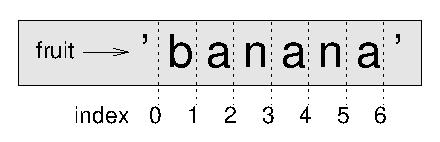
\includegraphics[scale=0.8]{figs/banana.eps}}
\caption{スライス・インデックス}
\label{fig.banana}
\end{figure}　
%
最初のインデックス（コロンの前）を省略すると、スライスは先頭の文字からとなる。
また二番目のインデックスを省略すると文字列の最後までとなる。
\begin{verbatim}
>>> fruit[:3]
'ban'
>>> fruit[3:]
'ana'
\end{verbatim}
最初のインデックスが二番目より等しいか大きいと{\bf 空文字列（empty string）}を返す。
これは二つの引用符で表現される：
\begin{verbatim}
>>> fruit = 'banana'
>>> fruit[3:3]
''
\end{verbatim}
空文字列は文字を一つも含まないので文字列の長さは0であるが、他の性質は普通の文字列と同じである。\par
同様な例として{\tt fruit[:]}は何を意味するだろうか？試して確認せよ。
%
\section{文字列は変更不可}
文字列の一部を変更しようとして以下のような代入を試みたとする：
\begin{verbatim}
>>> greeting = 'Hello World!'
>>> greeting[0] = 'J'
TypeError: 'str' object does not support item assignment
\end{verbatim}
ここで「オブジェクト」は文字列、「アイテム」は文字列の中の代入しようとした文字である。
この段階ではオブジェクト（object）とは値と同じものであるとしておく。後にこの定義は再吟味したい（10.10節）。\par
ここでのエラーの理由は文字列は{\bf 変更不可（immutable）}であることから来ている。
一旦作成した文字列は変更してはいけない。上の例で最良の解決は新しい文字列を生成することだ：
\begin{verbatim}
>>> greeting = 'Hello, world!'
>>> new_greeting = 'J' + greeting[1:]
>>> new_greeting
'Jello, world!'
\end{verbatim}
この例では新しい文字と{\tt greeting}のスライスしたものが連結されている。これでは元々の{\tt greeting}には何も変更もない。
%
\section{探索}
次ぎのプログラムは何をしているのだろうか？
\begin{verbatim}
def find(word, letter):
    index = 0
    while index < len(word):
        if word[index] == letter:
            return index
        index = index + 1
    return -1
\end{verbatim}
ある意味で、{\tt find}は{\tt []}演算子と逆の効果を持つ。
インデックスに従って対応する文字を取り出す替わりに文字を受け取り、その文字を有するインデックスを返すわけである。
文字が存在しないと{\tt -1}を返す。\par
また、この例がループの途中で{\tt return}文があるかたちの最初のものである。
もし{\tt word[index] == letter}が成立するとループが中断され{\tt return}文が実行される。
問題の文字が文字列に存在しないとプログラムは通常のように戻り値{\tt -1}で関数を終了する。 \par
配列を横断的に検査し、探しているものが見つかったら{\tt return}が実行されるといった計算パターンは{\bf 探索（search）}と呼ばれている。\par
練習問題として、関数{\tt find}を第三の仮引数を持つように修正せよ。この第三仮引数は探索を始めるインデックスの値である。
%
\section{ループ処理とカウンタ変数}
以下の関数はある文字が文字列の中に何回現れるか調べるプログラムである：
\begin{verbatim}
word = 'banana'
count = 0
for letter in word:
    if letter == 'a':
        count = count + 1
print(count)
\end{verbatim}
この例は{\bf カウンタ（counter）}と呼ばれるプログラムパターンを例示したことになる。
変数{\tt count}は{\tt 0}で初期化され、文字が発見される毎にインクリメントされる。
ループが終了すると結果、つまり文字{\tt 'a'}が出現する回数が表示される。 \par
練習問題として、上のプログラムをカプセル化して関数{\tt count}を作成せよ。
この関数は仮引数として文字列と探索文字を持つものとする。
それが済んだら関数{\tt count}を前節の第三の仮引数を持つ{\tt find}関数を使うように修正せよ。
%
\section{文字列メソッド}
文字列は各種の演算を実行するためのメソッドを提供している。
メソッドは関数と似ている、つまり引数を受け取り、戻り値を返す。
しかし、構文が異なっている。例えば、メソッド{\tt upper}は文字列を受け取り、全てを大文字にした文字列を返す。\par
通常の関数の構文、{\tt upper(word)}の替わりにメソッドの構文{\tt word.upper()}を使う。
\begin{verbatim}
>>> word = 'banana'
>>> new_word = word.upper()
>>> new_word
BANANA
\end{verbatim}
ドット記法の形式はメッソド{\tt upper}とそのメッソドを適用する文字列、{\tt word}を特定している。
空の丸括弧はこのメソッドが引数を何も取らないことを示している。\par
メソッドの呼び出しは{\bf 発動（invocation）}と呼ばれる。今の場合は{\tt word}に対して{\tt upper}を発動させたと言えばよい。\par
明らかになるように、文字列に対する{\tt find}というメソッドは関数として書いた{\tt find}と極めて類似した処理をするものである：
\begin{verbatim}
>>> word = 'banana'
>>> index = word.find('a')
>>> index
1
\end{verbatim}
この例では{\tt word}に対して{\tt find}を探索する文字を引数として渡して発動している。\par
メソッド{\tt find}は実際にはもっと複雑な処理ができる。引数は一文字でなく、文字列で構わない。
\begin{verbatim}
>>> word.find('na')
2
\end{verbatim}
また、第二の引数を付けることも可能で、この引数は探索を開始するインデックスを意味している：
\begin{verbatim}
>>> word.find('na', 3)
4
\end{verbatim}
これは{\bf 選択的な引数（optional argument）}の一例である。
更に、第三の引数も取れる。これは探索を止めるインデックスを意味している：
\begin{verbatim}
>>> name='bob'
>>> name.find('b', 1, 2)
-1
\end{verbatim}
この探索は失敗に終わっている。
なぜなら、探索区間の１から２まで（２は含まれない）の間に文字{\tt 'b'}はないからである。\\
%
\section{{\tt in}演算子}
英単語{\tt in}の表式で表現される演算子は二つの文字列を比較し、
最初の文字列が第二の文字列に含まれているときには{\tt True}を返すブール代数演算子である：
\begin{verbatim}
>>> 'a' in 'banana'
True
>>> 'seed' in 'banana'
False
\end{verbatim} \par
この演算子の例として、二つの文字列に共通に含まれている文字を表示する関数を示す：
\begin{verbatim}
def in_both(word1, word2):
    for letter in word1:
        if letter in word2:
            print(letter)
\end{verbatim}
変数の名前をうまく取っておくと、Pythonのプログラムは英文を読むように読める。
この{\tt for}ループは「第一の文字列になかにある各文字が第二の文字列の中にあるときにはその文字を{\tt print}する」と読める。
この関数を{\tt 'apples'}と{\tt 'oranges'}に適用すると以下のようになる：
\begin{verbatim}
>>>in_both('apples', 'oranges')
a
e
s
\end{verbatim}
%
\section{文字列の比較}
比較演算子は文字列にも適用できる。二つの文字列が一致しているかどうかを調べるには
\begin{verbatim}
if word == 'banana':
    print('All right, bananas.')
\end{verbatim} \par
他の比較演算子もアルファベット順に単語を並べるのに有効だ：
\begin{verbatim}
if word < 'banana':
    print('Your word, ' + word + ', comes before banana.')
elif word > 'banana':
    print('Your word, ' + word + ', comes after banana.')
else:
    print('All right, bananas.')
\end{verbatim}
Pythonは大文字、小文字の扱いを普通人々がするようには処理しない。
大文字で始まる全ての単語は小文字で始まる単語の前にくる。Pineappleとbananaを比較すると以下のよな表示になる：
\begin{verbatim}
Your word, Pineapple, comes before banana.
\end{verbatim} \par
これに対処する一般的な方法は文字列を標準化された形、例えば全てを小文字に変換した後に比較することである。
手榴弾（Pineapple）で武装した人に対処しなければならないときのためにこのことを記憶しておくとよい。
%
\section{デバッギング}
配列の横断的な処理をするとき、その処理の初めと終わりを正しく選ぶことには注意が必要だ。
以下は二つ単語を調べ、一つが他の逆順に並べたものであるときには{\tt True}を戻す関数の一例である。
しかし、二つのエラーを含んでいる：
\begin{verbatim}
def is_reverse(word1, word2):
    if len(word1) != len(word2):
        return False

    i = 0
    j = len(word2)

    while j > 0:
        if word1[i] != word2[j]:
            return False
        i = i + 1
        j = j - 1

    return True
\end{verbatim}
最初の{\tt if}文は二つの単語の長さが等しいかどうか調べている。
そうでなければ{\tt False}を戻り値として関数は終了する。
従ってこれ以降は二つの単語の長さは同じとして処理できる。これは6.8節で議論した保護回路の一例である。\par
変数{\tt i}、{\tt j}はインデックスである。{\tt i}は{\tt word1}を前方、{\tt j}は{\tt word2}を後方に横断的にサーベイする。
二つの文字が同じでないと、その場で{\tt False}を戻り値として関数は終了する。
ループの全過程を終了して抜けてきた場合は{\tt True}を戻り値として関数は終了する。 \par
単語potsとstopを使ってこの関数をテストする。
{\tt True}が期待されるが、インデックスが領域外という{\tt IndexError}が出る：
\begin{verbatim}
>>>is_reverse('pots', 'stop')
  File "is_reverse.py", line 9, in is_reverse
    if word1[i] != word2[j]:
IndexError: string index out of range
\end{verbatim}
このようなときに私が最初にやることは、このエラーが発生する直前でこれらの二つのインデックスの値を表示させてみることである。
\begin{verbatim}
    while j > 0:
        print(i, j)  #ここで印刷
        if word1[i] != word2[j]:
            return False
        i = i + 1
        j = j - 1
\end{verbatim}
実行してみると、新たな情報が得られるはずだ：
\begin{verbatim}
>>>is_reverse('pots', 'stop')
0 4...
IndexError: string index out of range
\end{verbatim}
ループの最初でjの値が4になっているこのが、この値は文字列{\tt 'pots'}では範囲外になる。
この文字列の最後の文字を示すインデックスの値は{\tt 3}で、{\tt j}の最初の値は{\tt len(word2)-1}である。\par
そのように修正して、実行すると以下になる：
\begin{verbatim}
>>>is_reverse('pots', 'stop')
0 3
1 2
2 1
True
\end{verbatim}
今回の場合は正しい結果になったが、ループは三回しか回っていない。おかしい。
このようなときは、この関数の状態図を書いてみるとよい。図\ref{fig.state4}は{\tt is\_reverse}関数の例で第一回目の繰り返し時の状態図である。
%
\begin{figure}[ttbp]
\centerline
{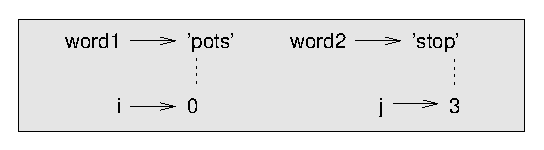
\includegraphics[scale=0.8]{figs/state4.eps}}
\caption{状態図}
\label{fig.state4}
\end{figure}
%
私はフレーム内の変数が持つ値を表示する場所に少し工夫を施した。
インデックス{\tt i}、{\tt ｊ}が文字列{\tt word1}、{\tt word2}のどの文字を指しているかが分かるようにその値と文字を点線で結んだ。\par
この図を紙に書いて繰り返し毎にインデックス{\tt i}、{\tt j}がどのような値をもつのか調べ
、関数{\tt is\_reverse}が持つ第二のエラーを修正せよ。
%
\section{語句}
\begin{description}

\item[オブジェクト（object）：] 変数が参照するあるもの（訳注：定義に対してその実体）。
%\index{object}

\item[配列（sequence）：] 整数インデックスによって同定される順序立った変数の組。.
%\index{sequence}

\item[アイテム（item）：] 配列の一要素。
%\index{item}

\item[インデックス（index）：] 文字列のような配列内の要素を選択ために使う整数値。
%\index{index}

\item[スライス（slice）：] インデックスの範囲指定で取り出された文字列の一部。
%\index{slice}

\item[空文字列（empty string）：] 二つの引用符で表現された文字を含まない長さ0の文字列。
%\index{empty string}

\item[変更不可（immutable）：] 文字列の要素を代入できない性質。
%\index{immutability}

\item[横断処理（traversal）：] 似たような操作を配列の端から端まで繰り返し行う。
%\index{traversal}

\item[探索（search）：] 捜していたものが見つかったときに停止する横断処理の一形態。
%\index{search pattern}
%\index{pattern!search}

\item[カウンタ（counter）：] 何か数えるために使われる変数。通常は0で初期化され、その後インクリメントされる。
%\index{counter}

\item[発動（invocation）：] メソッドを呼ぶ文。
%\index{invocation}

\item[選択的な引数（optional argument）：] 関数やメソッドで必ずしも必須としない引数。

\end{description}
%
\section{練習問題}

\noindent
{\bf 練習問題\tp.1} 文字列に対する各種のメソッドについて、\\
\url{http://docs.python.org/3/library/stdtypes.html#string-methods}をよく読み理解を深めよ。
{\tt strip}や{\tt replace}の使い方を実際にやってみることは有益かもしれない。\par
ドキュメンテーションは若干混乱するかもしれない構文規則の表現になっているかもしれない。例えば{\tt find}こうだ： 
\begin{verbatim}
find(sub[, start[, end]])
\end{verbatim}
角括弧は選択項目である。だから、{\tt sub}は必修だが、{\tt start}は選択項目であり、
{\tt start}を選択しても{\tt end}は選択項目である。\\

\noindent
{\bf 練習問題\tp.2} 8.7節に作成した{\tt count}と類似した機能を持つメソッド{\tt count}がある。
このメソッドのドキュメントをよく読み、文字列{\tt 'banana'}に対して発動させ文字列に含まれる{\tt 'a'}の個数を表示せよ。\\

\noindent
{\bf 練習問題\tp.3} 文字列スライスは第三の引数を受け取ることができる。
この第三の引数はスライスを何文字毎（ステップサイズ）にするかを指示するものである。
ステップサイズが2であるということは、文字列内の文字を一つ置きに拾うことであり、3であると、三つ毎になる。
\begin{verbatim}
>>> fruit = 'banana'
>>> fruit[0:5:2]
'bnn'
\end{verbatim}
このステップサイズを-1にすると後からのスライスになる。
だからスライス[::-1]とするとその文字列の逆順の文字列が得られる。
これを使って練習問題6.6で作成した文字列が回文である調べる関数{\tt is\_palidrome}の一行版を作成せよ。\\

\noindent
{\bf 練習問題\tp.4} 以下の関数はいずれも文字列が小文字を含んでいるかを調べる意図に作成したものであるが、
いずれも問題を含んでいる。各々の関数が実際にしていることを述べよ（関数に文字列を渡すとして）。
\begin{verbatim}
def any_lowercase1(s):
    for c in s:
        if c.islower():
            return True
        else:
            return False

def any_lowercase2(s):
    for c in s:
        if 'c'.islower():
            return 'True'
        else:
            return 'False'

def any_lowercase3(s):
    for c in s:
        flag = c.islower()
    return flag

def any_lowercase4(s):
    flag = False
    for c in s:
        flag = flag or c.islower()
    return flag

def any_lowercase5(s):
    for c in s:
        if not c.islower():
            return False
    return True
\end{verbatim}

\noindent
{\bf 練習問題\tp.5} シーザー暗号法は各文字をアルファベットで同一文字分文字を「回転」させる意味で微かに暗号のかたちを取っている。
文字を回転させるとはアルファベットのなかでずらし、文字Zを越えたときは先頭Aに戻るように折り返す操作である。
だから、文字'A'を３だけ回転させると文字'D'になり、'Z'は１だけ回転させると'A'になる。\par
単語の回転ではその単語を構成する各文字を同一の量だけ回転させる。例えば、``cheer"を7だけずらすと``jolly"になり、``melon"を
10だけずらすと``cubed"になる。映画``2001:Space Odyasey"（｛2001年宇宙の旅」）では、宇宙船内のコンピュータ（人工知能）は``HAL"と呼ばれているが、その名前を{\tt -1}
だけ回転させると``IBM"となる。

関数{\tt rotate\_word}を作成せよ。
この関数は文字列と整数を仮引数として持つ。
文字列の各文字を整数で指定された量だけ「回転」させ、その結果の文字列を戻り値とする関数である。\par
文字を文字コードに変換する組み込み関数{\tt ord}や
文字コードを文字に変換する組み込み関数{\tt chr}を使ってもよい。 
アルファベットの各文字はアルファベットの順に符号化されている。例えば
\begin{verbatim}
>>> ord('c') - ord('a')
2
\end{verbatim}
アルファベットの{\tt 'c'}はアルファベットの二番目の文字である。しかし大文字の数値コードは小文字と異なることに注意。\par
インタネットに対する潜在的に悪意のあるジョークが回転文字数が13であるシーザー暗号法を使った
ROT13にコード化されていることがある。あまり気にならなければ、それを見つけ元に戻してみよう。\\
解答例：\url{https://thinkpython.com/code/rotate.py}.
%
\chapter{事例研究：単語あそび}
この章ではある種の性質を持つ英単語を探索するといった単語パズルを解くことを含むこの本の二番目の事例研究
である。例えば、英単語の中で最長の回語は何か、また文字がまたアルファベットの順序で現れる単語にどんなものがあるかと
いった問題である。また新しい問題を既存の解決済みの問題に帰着させるというもう一つのプログラム開発手法を紹介する。
\section{単語リストの読み込み}
この章の演習では英単語のリストが必要だ。英単語のリストはWebで入手可能なものが沢山あるが、
我々の目的に最適なものはMobyレキシコンプロジェクト（\url{http://wikipedia.org/wiki/Moby_Project}をみよ）の
一部としてGrady Wardによって収集され、公開されている英単語リストがその一つである。\par
それは公式のクロスワードパズルや他の英単語ゲームに使える113,809個の英単語リストである。
この集録は{\tt 113809f.fic}という名前のファイルになっているが、
もっと簡単な名前、.{\tt words.txt}で\url{https://thinkpython.com/code/words.txt}からダウンロードできる。 \par
このファイルは単純なテキストファイルであるので、テキストエディタで閲覧できるし、Pythonで読むこともできる。
組み込み関数{\tt open}の引数ファイル名を与え実行する
と{\bf ファイルオブジェクト（file object）}を返してくる。これを使ってファイルを読むことができる：
\begin{verbatim}
>>> fin = open('words.txt')
\end{verbatim}
変数{\tt fin}は入力に使うファイルオブジェクトによく使われる名前である。
モード{\tt 'r'}は読み込みモードでファイルがオープンされたことを示す（その逆は書き込みモードで{\tt 'w'}である）。\par
ファイルオブジェクトは読み込みのためのいくつかのメソッドを提供している。
その一つは{\tt readline}でこれは文字を改行記号に達すまで読み込み、その結果を文字列として返すメソッドである：
\begin{verbatim}
>>> fin.readline()
'aa\r\n'
\end{verbatim}
このリストの第一番目の単語は``aa"である。これは溶岩の一種である。符号{\verb"\r\n"}は二つ特殊記号、
キャリージ・リターンと改行でこの単語を次ぎのものから分離するのに使われている。
ファイルオブジェクトは今ファイルのどこにいるのかの軌跡を保存している。だから、次ぎに{\tt readline}を実行すると次ぎの単語を読み出せる：
\begin{verbatim}
>>> fin.readline()
'aah\r\n'
\end{verbatim}
次の単語は``aah"で、全く規則にあった単語である。
そんなに怪訝な様子で私をみないでください。二つの特殊記号が邪魔ならば、文字列メッソド{\tt strip}を使って取ってしまうこともできる：
\begin{verbatim}
>>>line = fin.readline()
>>>word = line.strip()
>>>word
aahed
\end{verbatim} \par
{\tt for}ループの一部にファイルオブジェクトを使うこともできる。
以下のプログラムは{\tt words.txt}を読み込み、一行に一単語毎に表示するものである：
\begin{verbatim}
fin = open('words.txt')
for line in fin:
    word = line.strip()
    print(word)
\end{verbatim}


\section{練習問題}
これからの練習問題の解答は次の節にあるが、答えをみる前に一度は解答を試みてほしい。\\

\noindent
{\bf 練習問題\tp.1} ファイル{\tt words.txt}を読み、
単語の長さが20（特殊文字を含めないで）以上ある単語のみを表示するプログラムを作成せよ。\\

\noindent
{\bf 練習問題\tp.2} Ernst Vincent Wrightは1939年にGadsbyというタイトルの50,000単語の小説を出版した。
この本は文字'e'を全く含んでいない。文字'e'は英語では最も頻度の高い文字であるので、この作業は簡単ではない。
\begin{quote}
In fact, it is difficult to construct a solitary thought without using that most common symbol, it is slow going at first, but caution and hours of training can gradually gains facility.
\end{quote}
この位で止めておこう。 \par
与えられた単語が文字{\tt 'e'}を一つも含んでいないと{\tt True}を返す関数{\tt has\_no\_e}を作成せよ。\par
練習問題{\tp.1}のプログラムを単語が{\tt 'e'}を含んでいないときにのみ単語を表示するように変更し、
文字{\tt 'e'}を含まない単語の全単語中に占めるパーセントを計算しなさい。\\

\noindent
{\bf 練習問題\tp.3} 文字列と文字を引数とする関数{\tt avoids}を作成せよ。
この関数はその文字列に該当する文字が一つも含まれていないときは{\tt True}を返す。 \par
ユーザから入力された文字に対して、この文字を一つも含まない単語を表示するように練習問題{\tp.1}のプログラムを変更せよ。\par
また、このような文字5個を使ったときに排除される単語数が最少になるような5個の組み合わせを見つけることができるか？\\

\noindent
{\bf 練習問題\tp.4} 文字列と文字の組み合わせ（文字列）を引数とする関数{\tt uses\_only}を作成せよ。
この関数はこの文字列がこの組み合わせ文字でのみ構成されているときは{\tt True}を返す。
また、組み合わせ文字、``acefhlo"のみを使って一つの文を作れるかな？``Hoe alfalfa"（アルファルファを刈り取る）以外には？ \\

\noindent
{\bf 練習問題\tp.5} 文字列と要求される文字の組み合わせ（文字列）を引数とする関数{\tt uses\_all}を作成せよ。
この関数はこの文字列が要求される文字を全て少なくとも一回は使っているときは{\tt True}を返す関数である。
全ての母音``aeiou"を使うような単語は何個位あるのだろうか``aeiouy"ではどうかな？ \\

\noindent
{\bf 練習問題\tp.6} 引数として受け取った単語の中の文字の並びがアルファベット順
（同じ文字が並ぶのはよいとする）に並んでいるときTrueを返す関数{\tt is\_abecedarian}を作成せよ。
この条件を満たす単語は何個位あるのだろうか？
%
\section{探索}
前節で取り上げた練習問題全ては共通した要素を持っている。
それは8.6節でみた探索パターンで解答できることである。最も簡単な例は以下である：
\begin{verbatim}
def has_no_e(word):
    for letter in word:
        if letter == 'e':
            return False
    return True
\end{verbatim}
この{\tt for}ループは単語中の文字を横断的に探索する。
もし文字``e"が見つかれば直ちに{\tt False}を返し関数は終了する。そうでなければ次ぎの文字に移る。
ループを通常の姿で抜けたことは文字``e"を一つも含まないことなので{\tt True}を返す。 \par
関数{\tt avoids}は関数{\tt has\_no\_e}を一般化したものであるが、プログラムの構造は同じだ：
\begin{verbatim}
def avoids(word, forbidden):
    for letter in word:
        if letter in forbidden:
            return False
    return True
\end{verbatim}
文字の組み合わせ文字列{\tt forbidden}内の文字を一つでも含んでいると直ちに
{\tt False}を返し関数は終了する。ループを通常の姿で抜けると{\tt True}を返す。 \par
関数{\tt uses\_only}も条件は逆だが、同じ構造をしている。
\begin{verbatim}
def uses_only(word, available):
    for letter in word:
        if letter not in available:
            return False
    return True
\end{verbatim}
禁止文字の組み合わせの替わりに、利用可能な文字の組み合わせを使う。
利用可能文字以外の文字がみつかったら直ちに{\tt False}を返して関数は終了する。\par
関数{\tt uses\_all}では単語と組み合わせ文字の役割を逆にする。
\begin{verbatim}
def uses_all(word, required):
    for letter in required:
        if letter not in word:
            return False
    return True
\end{verbatim}
単語（{\tt word}）の中の文字を横断的に調べる替わりに、
要求された文字の組み合わせ（{\tt required}）の中の文字を横断的に調べる。
要求された文字が一つでも欠けていたら直ちにFalseを返し関数を終了する。\par
本物のコンピュータ科学者のように考えるのであれば、{\tt uses\_all}は前の解いた問題の新たな例証にすぎないことを認識するはずだ。
そして以下のように書くだろう：
\begin{verbatim}
def uses_all(word, required):
    return uses_only(required, word)
\end{verbatim} \par
この例は{\bf 解決済み問題への帰着（reduction to a previously solved problem）}と言われるプログラム開発法の一例である。
そこでは当該の問題がそれまで解決した問題の新たな例証にすぎないことを認識し、既に開発した解法を適用する。
%
\section{インデックス付きループ}
前節のプログラムではforループを伴う関数を作成した。文字列の中の任意の位置にある文字なので、そのループはインデックスが付くものではなかった。 \par
関数{\tt is\_abecedarian}では隣接する文字との比較が入るので、{\tt for}ループは少し注意が必要だ。
\begin{verbatim}
def is_abecedarian(word):
    previous = word[0]
    for c in word:
        if c < previous:
            return False
        previous = c
    return True
\end{verbatim} 
再帰関数を使う版は以下のようだ：
\begin{verbatim}
def is_abecedarian(word):
    if len(word) <= 1:
        return True
    if word[0] > word[1]:
        return False
    return is_abecedarian(word[1:])
\end{verbatim} 
{\tt while}ループを使う版は以下のようだ：
\begin{verbatim}
def is_abecedarian(word):
    i = 0
    while i < len(word)-1:
        if word[i+1] < word[i]:
            return False
        i = i + 1
    return True
\end{verbatim} 
このループは{\tt i=0}から始まり、{\tt i=len(word)-1}で終わる。
ループを回る毎に第{\tt i}番目の文字（これが現在の文字）と第{\tt i+1}番目の文字（これが次ぎの文字）とが比較される。
このループを失敗なしで通過すると問題の単語はテストを合格したことになる。
この処理が正しいことを確認するために、``flossy"という単語を例に手作業をしてみる。この単語の長さは6である。
従ってこのループを最後に回るときのiの値は4である。この値は後から二番目の文字を示す。
この最後のループではこの後から二番目の文字と最後の文字を比較することになる。\par
以下は関数{\tt is\_palindrome}（6.6節参照のこと）を二つのインデックスを使う版である：
\begin{verbatim}
def is_palindrome(word):
    i = 0
    j = len(word)-1

    while i<j:
        if word[i] != word[j]:
            return False
        i = i+1
        j = j-1
    return True
\end{verbatim}
また、この問題は前に解いた問題の一つの例証にすぎないことを見抜けば、以下のように書くこともできる：
\begin{verbatim}
def is_palindrome(word):
    return is_reverse(word, word)
\end{verbatim}
と8.11節の{\tt is\_reverse}を使ってか書ける。
%
\section{デバッギング}
プログラムをテストすることは手強いものである。この章に現れた関数は手作業でテストできるので比較的易しいものである。
それでも、潜在的なエラーの全てを摘出するために必要な単語のセットを選ぶことは困難または不可能に近い問題である。 \par
関数{\tt has\_no\_e}を例にしてみよう。'e'を含む単語のなかで、先頭にある単語、最後にある単語、中間にある単語でテストする必要がある。
また、長い単語、短い単語、空文字列のような極端に短い単語も調べる必要がある。
空文字列は{\bf 特別な例（special case）}の一例でときとしてエラーが潜むことがある。\par
テストとして用意した単語の他に{\tt words.txt}のような既存の単語リストでプログラムをテストすることもできる。
出力を調べることでエラーを見つけることができるかもしれないが、注意したいのは摘出したエラーはそのリストに含まれていない単語ではなく、
含まれている単語に関してのみであることだ。 \par
一般にテストすることはバグを探すのに有効だが、テストに使うよいセットを用意するのは容易ではない。
そして、たとえ用意できたとしても、プログラムが正しいことの確証を持つことはできない。\par
伝説的なコンピュータ科学者によれば
\begin{quote}
プログラムをテストすることはバグの存在を示すことには使えるが、決してバグがないことを示すことには使えない。\par
---エドガー ・ダイクストラ
\end{quote}
%
\section{語句}
\begin{description}

\item[ファイルオブジェクト（file object）：] 開かれたファイルを表現する値。.
%\index{file object}
%\index{object!file}

\item[解決済み問題への帰着（reduction to a previously solved problem）：] 既に解かれた問題の例証として表現することで問題を解く。
%\index{problem recognition}

\item[特別な例（special case）：] 典型的でなくまたは明白でない（そして正確に処理することができにくくみえる）検定用に使う例。.
%\index{special case}

\end{description}
%
\section{練習問題}
{\bf 練習問題\tp.7} この問題はラジオプログラムCar Talk　
(\url{http://www.cartalk.com/content/puzzlers})
で放送されたパズル名人を基礎とした問題である。
\begin{quote}
連続して二回同じ文字が続き、しかもこれが三回引き続いて起こるような単語を私にください。
それに近いような単語の例を示す。例えば、committeeつまり、{\tt c-o-m-m-i-t-t-e-e}。途中にこっそりとiが入っていることを除けば可成り近い例である。
また、Mississippiつまり、{\tt M-i-s-s-i-s-s-i-p-p-i}。もしもiを削除してもよいとすれば、まあ条件を満たす例になる。
しかし、上の条件を完全に満たす単語が一つある。しかも、私の知る得る限りではこれが唯一の単語だ。
条件をみたしている単語は多分500個近くあるかもしれないが、私はその一つしか知らない。さて、その単語は何か？
\end{quote}
この単語を見つけるプログラムを作成せよ。\\
解答例： \url{https://thinkpython.com/code/cartalk1.py} \\

\noindent
{\bf 練習問題\tp.8} これもCar Talkのパズル名人による。
 ((\url{http://www.cartalk.com/content/puzzlers}） 
\begin{quote}
先日ハイウエイをドライブしていた。そしてたまたま私の車の走行距離計が目に入った。
多くの走行距離計と同じで6桁の数字で走行距離がマイルを単位として表示されている。
従って、私の車が300,000マイル走ったのであると表示は{\tt 3-0-0-0-0-0}となる。
さて、あの日に私がみた走行計の文字は興味あるものであった。
最後の四桁の数字が回文になっていたのだ。つまり、それらは前から読んでも後から読んでも同じだったわけだ。
例えば、{\tt 5-4-4-5}は回文だ。
距離計は例えば{\tt 3-1-5-4-4-5}となっていたわけである。
ところが1マイル走って距離計をみると今度は最後の五桁が回文になっていた。
例えば、{\tt 3-6-5-3-5-6}ようだ。
さらに1マイル走って距離計をみると六桁の内中間の四文字が回文になっていた。
さらに驚くことに、1マイル走って距離計をみるとなんと六桁全体が回文になっていた。問題は最初に眺めた距離計の表示は何か？
\end{quote}
六桁全ての数字をテストし、上の条件を満たす組み合わせを表示するPythonプログラムを書け。\\
解答例： \url{https://thinkpython.com/code/cartalk2.py} \\

\noindent
{\bf 練習問題\tp.9} これもまたCar Talkからである。探索手法で解けるはずだ。
(\url{http://www.cartalk.com/content/puzzlers}):
\begin{quote}
母親を最近に訪ねた、そして私の年齢の二桁の数字が母のそれと逆順になっていることに気が付いた。
例えば、母が73で、私が37といった具合だ。このような状況がどの位の頻度で起ったのか話題になったが、
話が横道に逸れてしまい、答えを得る機会がなかった。\par
自宅に帰った後に、この年齢の逆順はこれまで6回起きていたことが分かった。
また、幸運ならば、この数年中にこの逆順が起こることも分かった。
さらに、充分に幸運ならばこの逆順はさらにもう一度訪れるだろうと期待できた。
従って（母が99歳になるまで）8回の頻度でこの現象が起きたことになる。
問題は、私の現在の年齢はいくつか？
\end{quote}
この問題を探索の問題として解くPythonのプログラムを作成せよ。 
組み込み関数{\tt zfill}を使ってもよい(訳注：{\tt zfill}は数字の先頭を0で埋める。{\tt '5'.zfill(4)}のように使う)。\\
解答例：\url{https://thinkpython.com/code/cartalk3.py}
%
\chapter{リスト}
この章ではPythonで扱える最も便利な組み込み型の一つであるリストを取り上げる。さらにオブジェクトについて学び、同一のオブジェクトを一つ以上
の変数で参照したとき何が起こるか調べる。
\section{リストは配列である}
文字列と同じように{\bf リスト（list）}も値の配列である。
文字列の値が文字であるのに対して、リストの値は任意の型で構わない。
リストの値は{\bf 要素（elements）}または{\bf アイテム（items）}と呼ばれる。 \par
リストを生成する方法はいくつもあるが、最も簡単な方法は要素を角括弧（{\tt [ と ]}）で括ることである：
\begin{verbatim}
[10, 20, 30, 40]
['crunchy frog', 'ram bladder', 'lark vomit']
\end{verbatim}
一番目の例は四つの整数のリストである。二番目は三つの文字列のリストである。
一つのリストの要素は同じ型にする必要はない。以下のリストは文字列、浮動小数点数、整数、それに、（あれ！）リストを含んでいる：
\begin{verbatim}
['spam', 2.0, 5, [10, 20]]
\end{verbatim}
リストの中にリストがあると{\bf 入れ子のリスト（nested list）}になる。\par
要素を何も含まないリストは空リストと呼ばれ、空の角括弧{\tt []}で生成できる。
予想したであろうように、リストを変数に代入できる：
\begin{verbatim}
>>> cheeses = ['Cheddar', 'Edam', 'Gouda']
>>> numbers = [17, 123]
>>> empty = []
>>> print(cheeses, numbers, empty)
['Cheddar', 'Edam', 'Gouda'] [17, 123] []
\end{verbatim}
%
\section{リストは変更可能}
リストの要素にアクセスする構文は文字列の中の文字にアクセスするときと同じである。
つまり、角括弧を使う。角括弧の中の表式はインデックスを表現する。インデックスは{\tt 0}から始まることに注意してほしい。
\begin{verbatim}
>>> cheeses[0]
Cheddar
\end{verbatim} \par
文字列と異なり、リストは変更可能である。代入文で角括弧の演算が左に現れるとそれはリストのある要素への代入を表現する：
\begin{verbatim}
>>> numbers = [42, 123]
>>> numbers[1] = 5
>>> numbers
[42, 5]
\end{verbatim}
リスト{\tt numbers}の第一要素は{\tt 123}だったものが{\tt 5}になった。\par
リストはインデックスと要素との間にある関係と考えることもできる。この関係は{\bf マッピング（mapping）}とも呼ばれている。
つまり各インデックスは要素の一つを「写像」しているとみることができる。
図\ref{fig.liststate}はリスト{\tt cheeses}, {\tt numbers}, {\tt empty}の状態図を示している。
%
\begin{figure}[htbp]
\centerline
{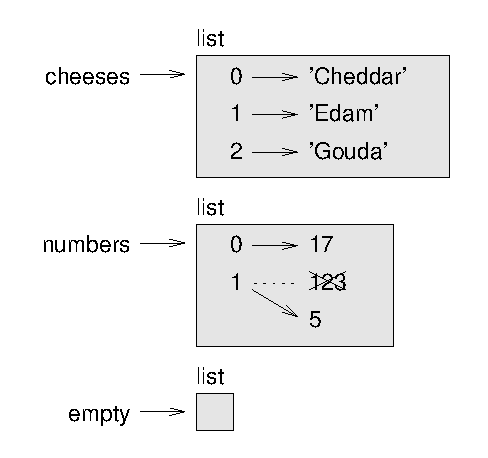
\includegraphics[scale=0.8]{figs/liststate.eps}}
\caption{状態図}
\label{fig.liststate}
\end{figure}
これらのリストは箱によって表現されている。その箱の外側にはリストの名前が、内側にはその要素が書かれている。
{\tt cheeses}は要素が{\tt 0}, {\tt 1}, {\tt 2}のインデックスを持つ一つリストを参照している。
{\tt numbers}は二つの要素を持つが、図はその第二要素は{\tt 123}から{\tt 5}に変更されたことを示している。
{\tt empty}は空リストを参照している。\par
リストのインデックスは文字列のそれと同じように働く。つまり
\begin{itemize}
\item 任意の整数表式がインデックスとして使える。
\item もし存在しない要素を呼び出したり、書き出したりすると{\tt IndexError}になる。
\item もしもインデックスの値が負であるとすると、それはリストの後の要素からカウントしている意味だ。
\end{itemize} \par
{\tt in}演算子もリストにそのまま機能する。
\begin{verbatim}
>>> cheeses = ['Cheddar', 'Edam', 'Gouda']
>>> 'Edam' in cheeses
True
>>> 'Brie' in cheeses
False
\end{verbatim}
%
\section{リストの横断的処理}
リストの要素を横断的にアクセスする一般的な方法は{\tt for}ループを使うものである。
構文は文字列の場合と同じである：
\begin{verbatim}
for cheese in cheeses:
    print(cheese)
\end{verbatim}
これはリストの要素を読み出すのみのときの場合である。
要素の書き込みや更新をしたいときにはインデックスが必要になる。
この場合の一般的な方法は{\tt range}関数を使うものである：
\begin{verbatim}
for i in range(len(numbers)):
    numbers[i] = numbers[i] * 2
\end{verbatim}
このループでリストの各要素を横断的に更新できる。
関数{\tt len}でリストの要素の数を出し、関数{\tt range}で{\tt 0}から{\tt n-1}までの数のリストを生成する。
ここで{\tt n}は問題のリストの長さである。ループが回る毎にiは次ぎの要素に対応するインデックスの値を持つ。
代入文ではiは古い要素に値を読むことに使われ、新しい値を代入することにも使われている。\par
空リストに対するforループでは本体は一度も実行されない：
\begin{verbatim}
for x in []:
    print('This never happens.')
\end{verbatim} \par
リストの中にリストを含ませることもできるが、そのリストは一つの要素としてカウントされる。
従って以下のリストの要素の数は4である。
\begin{verbatim}
['spam', 1, ['Brie', 'Boquefort', 'Poi le Veq'], [1, 2, 3]]
\end{verbatim}
%
\section{リストに対する演算}
演算子{\tt +}はリストの連結を実現する。
\begin{verbatim}
>>> a = [1, 2, 3]
>>> b = [4, 5, 6]
>>> c = a + b
>>> c
[1, 2, 3, 4, 5, 6]
\end{verbatim}
同じように演算子{\tt *}は与えられた回数だけ繰り返したリストを生成する。
\begin{verbatim}
>>> [0] * 4
[0, 0, 0, 0]
>>> [1, 2, 3] * 3
[1, 2, 3, 1, 2, 3, 1, 2, 3]
\end{verbatim}
最初の例では{\tt [0]}を4回繰り返す。二番目では{\tt [1, 2, 3]}を3回繰り返す。
%
\section{リストのスライス}
スライス演算もリストに適用できる：
\begin{verbatim}
>>> t = ['a', 'b', 'c', 'd', 'e', 'f']
>>> t[1:3]
['b', 'c']
>>> t[:4]
['a', 'b', 'c', 'd']
>>> t[3:]
['d', 'e', 'f']
\end{verbatim}
一番目のインデックスを省略すると、スライスは先頭から始まる。
二番目のインデックスを省略するとスライスは最後尾まで進行する。両インデックスを省略するとリスト全体がコピーされる。
\begin{verbatim}
>>> t[:]
['a', 'b', 'c', 'd', 'e', 'f']
\end{verbatim} \par
リストは更新可能だから、折り畳み、回転、変更の操作をする前にそのコピーを作っておくことは多々有益である。\par
スライス演算子を代入文の左辺で使うと、複数要素を更新できる：
\begin{verbatim}
>>> t = ['a', 'b', 'c', 'd', 'e', 'f']
>>> t[1:3] = ['x', 'y']
>>> t
['a', 'x', 'y', 'd', 'e', 'f']
\end{verbatim}
%
\section{リストメソッド}
Pythonはリストに適用できる各種のメソッドを提供している。例えば、{\tt append}は要素の追加に使う：
\begin{verbatim}
>>> t = ['a', 'b', 'c']
>>> t.append('d')
>>> t
['a', 'b', 'c', 'd']
\end{verbatim} \par
メソッド{\tt extend}はリストを引数として受け取り、その要素の全てをリストに追加する：
\begin{verbatim}
>>> t1 = ['a', 'b', 'c']
>>> t2 = ['d', 'e']
>>> t1.extend(t2)
>>> t1
['a', 'b', 'c', 'd', 'e']
\end{verbatim}
この場合リスト{\tt t2}の中味は変わらない。 \par
メソッド{\tt sort}はリストの要素を低位から高位に順に並べ替える：
\begin{verbatim}
>>> t = ['d', 'c', 'e', 'b', 'a']
>>> t.sort()
>>> t
['a', 'b', 'c', 'd', 'e']
\end{verbatim}
リストのメソッドは全て戻り値がない、だから{\tt None}を戻す。
もし間違って{\tt t=t.sort()}とすると、期待はずれの結果になる。
%
\section{写像・フィルタ・還元}
リストの要素を全て足そうと思ったら、以下のようにループを使うだろう：
\begin{verbatim}
def add_all(t):
    total = 0
    for x in t:
        total += x
    return x
\end{verbatim}
変数{\tt total}は0で初期化される。
変数{\tt x}はループを回る毎にリストtの要素を得る。
演算子{\tt +=}は変数の更新の操作の省略形である。{\bf 累積代入文（augmented assignment statement）}、
{\tt total += x}は{\tt total = total + x}と等価である。
ループが進むに連れて、{\tt total} は要素の和の累積になる。
このような機能のために用いられる変数は{\bf アキュームレイタ（accumulator）}と呼ばれる。\par
要素の全和を求めることは一般的なので、Pythonでは組み込み関数{\tt sum}を提供している：
\begin{verbatim}
>>> t = [1, 2, 3]
>>> sum(t)
6
\end{verbatim} \par
要素の列を一つの値にしてしまうような操作を{\bf 還元（reduce）}と呼ぶ。\par
ときとして他のリストを作成しつつ、リストを横断的に処理する必要がある。例えば
\begin{verbatim}
def capitalize_all(t):
    res = []
    for s in t:
         res.append(s.capitalize())
    return res
\end{verbatim}
変数{\tt res}は空リストとして初期化される。
ループが回る毎にオリジナルのリストの要素が処理され{\tt res}に追加される。
従って変数{\tt res}は別な種類のアキュームレイタとみなすことができる。
関数{\tt capitalize\_all}のような処理を{\bf 写像（map）}という。
ここではあるリストの全要素に同一の処理（{\tt capitalize()}）を施すからである。\par
もう一つの操作はリストの一部を選択して部分リストを作成するものである。
例として文字列のリストから大文字のみを含む要素を選択し、部分リストを作る問題を考える：
\begin{verbatim}
def only_upper(t):
    res = []
    for s in t:
         if s.isupper():
            res.append(s)
    return res
\end{verbatim}
メソッド{\tt isupper}は文字列が大文字のみを含んでいるとき{\tt True}を返す。\par
このような操作はリストの要素のなかで条件を満たすものだけを別なリストの
要素にするから{\bf フィルタ（filter）}と呼ばれる。\par
リストに対する操作で最も一般的なものはこれらの写像・フィルタ・還元を組み合わせたものである。
%
\section{要素の削除}
リストの要素を削除する方法はいくつかある。要素番号を知っているのであれば、{\tt pop}を使うことができる：
\begin{verbatim}
>>> t = ['a', 'b', 'c']
>>> x = t.pop(1)
>>> t
['a', 'c']
>>> x
b
\end{verbatim}
メソッド{\tt pop}はリストを修正し、削除した要素を返す。
もし{\tt pop}をインデックスなして使うと最後尾の要素を削除し、その要素を返す。\par
要素を戻す必要がなければ、{\tt del}演算子が使える：
\begin{verbatim}
>>> t = ['a', 'b', 'c']
>>> del t[1]
>>> t
['a', 'c']
\end{verbatim} \par
削除する要素を知っている（しかし、要素番号は不明）のであれば、メソッド{\tt remove}が使える：
\begin{verbatim}
>>> t = ['a', 'b', 'c']
>>> t.remove('b')
>>> t
['a', 'c']
\end{verbatim} \par
もし一つ以上の要素を一時に削除したいのであれば、スライス演算子で範囲を決め、{\tt del}演算子を使えばよい：
\begin{verbatim}
>>> t = ['a', 'b', 'c', 'd', 'e', 'f']
>>> del t[1:5]
>>> t
['a', 'f']
\end{verbatim}
スライスは第一番目のインデックスの要素から第二番目の要素まで選択する。注意、二番目のインデックスの要素は含まれない。\\
%
\section{リストと文字列}
文字列は文字の配列であり、リストは値の配列である。しかし、文字のリストは文字列とは異なる。\par
文字を要素とするリストに文字列を変換するには関数{\tt list}を使う：
\begin{verbatim}
>>> a = 'spam'
>>> t = list(a)
>>> t
['s', 'p', 'a', 'm']
\end{verbatim}
{\tt list}は組み込み関数であるので、変数名として避けるべきである。
また{\tt l}（エル）はあまりにも１と似ているので避け、{\tt t}を用いた。 \par
関数{\tt list}は文字列を文字に分解しリストにする。文字列を単語に分解するのは{\tt split}を使う：
\begin{verbatim}
>>> s = 'pining for the fjords'
>>> t = s.split()
>>> t
['pining', 'for', 'the', 'fjords']
\end{verbatim}
このメソッドに引数として{\bf 区切り文字（delimiter）}を与えることができる。
これで如何なる文字を使って単語に分割するかを指定できる。
\begin{verbatim}
>>> s = 'spam-spam-spam'
>>> delimiter = '-'
>>> t = s.split(delimiter)
>>> t
['spam', 'spam', 'spam']
\end{verbatim} \par
メソッド{\tt join}は{\tt split}の逆の操作だ。このメソッドは引数として文字列のリストを受け取り、要素の連結を作る
。{\tt join}は文字列のメソッドで区切り文字に対して発動される。リストはこのメソッドの引数として与える：
\begin{verbatim}
>>> t = ['pining', 'for', 'the', 'fjords']
>>> delimiter = ' '
>>> s = delimiter.join(t)
>>> s
'pining for the fjords'
\end{verbatim}
このばあいは空白を区切り文字として単語を接合する。区切り文字なして接合するには空文字{\tt ''}を区切り文字とすればよい。
%
\section{オブジェクトと値}
以下のような代入文を実行してみる：
\begin{verbatim}
>>> a = 'banana'
>>> b = 'banana'
\end{verbatim}
変数{\tt a}、{\tt b}とも同じ文字列を参照している。
%
\begin{figure}[htbp]
\centerline
{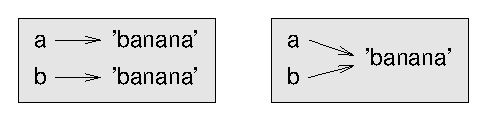
\includegraphics[scale=0.8]{figs/list1.eps}}
\caption{.状態図}
\label{fig.list1}
\end{figure}
%
しかし、この二つが同一の文字列を参照しているかどうかは不明である。図\ref{fig.list1}に示したように二つの可能性がある。
一つの可能性は、この二つは同じ値を持つが異なった{\bf オブジェクト（実体）（object）}を参照しているとするものだ。
他方は同一のオブジェクトを参照しているとするものである。
これをチェックするには{\tt is}演算子を使ってみればよい：
\begin{verbatim}
>>> a = 'banana'
>>> b = 'banana'
>>> a is b
True
\end{verbatim}
この例ではPythonは一つ文字列オブジェクトを生成し、変数{\tt a}、{\tt b}ともこれを参照している。\par
しかし、二つのリストでは、二つのオブジェクトが生成される：
\begin{verbatim}
>>> a = [1, 2, 3]
>>> b = [1, 2, 3]
>>> a is b
False
\end{verbatim}
従って状態図は図\ref{fig.list2}のようになる。
%
\begin{figure}[htbp]
\centerline
{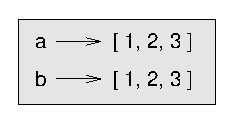
\includegraphics[scale=0.8]{figs/list2.eps}}
\caption{状態図}
\label{fig.list2}
\end{figure}
この場合二つのリストは同じ要素を持っているので{\bf 等価（equivalent）}であるという。
しかし異なったオブジェクトであるので{\bf 同一（identical）}ではない。同一である
二つのオブジェクトは等価であるが、等価である二つのオブジェクトは必ずしも同一ではない。\par
これまで「オブジェクト（実体）」と「値」を交換可能な言葉として使ってきたが、もう少し厳密に言うとこうなる。オブジェクトは値を持つ。
操作{\tt [1, 2, 3]}を行うとその要素が整数の値を持つリストオブジェクトが得られる。
もしも他のリストが同じ値を持っていたとすると、２つのリストは同じ値を持つというが、同一のオブジェクトではない。
%
\section{別名参照}
変数{\tt a}は一つのオブジェクトを参照し、{\tt b=a}という代入文を実行すると、二つの変数は同一のオブジェクトを参照することになる：
\begin{verbatim}
>>> a = [1, 2, 3]
>>> b = a
>>> b is a
True
\end{verbatim}
従って状態図は図\ref{fig.list3}のようになる。
%
\begin{figure}[htbp]
\centerline
{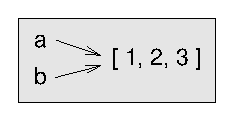
\includegraphics[scale=0.8]{figs/list3.eps}}
\caption{状態図}
\label{fig.list3}
\end{figure}
一つの変数にオブジェクトを代入することは{\bf 参照（reference）}という。
この例では一つのオブジェクトに対して二つ参照があることになる。
一つのオブジェクトに対して二つ以上の参照があるとき、このオブジェクトは{\bf 別名参照された（aliased）}オブジェクトという。\par
もしも別名参照されたオブジェクトが変更可能であるとすると、一つの別名に行った変更は他にも反映される：
\begin{verbatim}
>>> b[0] = 42
>>> a
[42, 2, 3]
\end{verbatim}
この振る舞いは利用できるときがあるが、エラーを起こしやすい。変更可能オブジェクトにたいする別名は避ける方が安全だ。
変更不可のオブジェクトでは問題は少ない。
\begin{verbatim}
>>> a = 'banana'
>>> b = 'banana'
\end{verbatim}
この例で変数{\tt a}、{\tt b}が同じ文字列を参照しているかどうかは殆ど問題にならない。
%
\section{リストを引数に使う}
リストを関数の引数として渡すと、その関数はそのリストの参照ができる。関数はこの仮引数としてのリストを変更するとこの関数の呼び手のリストも変更を受ける。
例えば、関数{\tt delete\_head}はリストの先頭の要素を削除する関数としよう：
\begin{verbatim}
>>> def delete_head(t):
	del t[0]
\end{verbatim}
この関数を使う：
\begin{verbatim}
>>> letters = ['a', 'b', 'c']
>>> delete_head(letters)
>>> letters
['b', 'c']
\end{verbatim}
仮引数{\tt t}と変数{\tt letters}とは同一のリストの別名参照である。これらのスタック図は\ref{fig.stack5}図のようになる。
%
\begin{figure}[htbp]
\centerline
{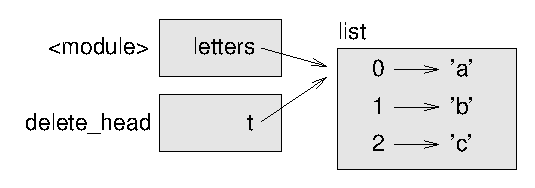
\includegraphics[scale=0.8]{figs/stack5.eps}}
\caption{スタック図}
\label{fig.stack5}
\end{figure}
%
このリストは二つのフレームで共用されているので中間に置いた。 \par
リストの変更を伴う操作と新たなリストを生成する操作を区別することは特別に重要だ。
例えば、メソッド{\tt append}はリストの変更を伴うが、演算子{\tt +}はあらたなリストの生成になる。
\begin{verbatim}
>>> t1 = [1, 2]
>>> t2 = t1.append(3)
>>> t1
[1, 2, 3]
>>> t2
None

>>> t4 = t1 + [4]
>>> t4
[1, 2, 3, 4]
\end{verbatim} \par
リストの変更を期待する関数を作ろうとするときもこの相異に注意が必要だ。
\begin{verbatim}
def bad_delete_head(t):
    t = t[1:]    #間違いだ
\end{verbatim}
スライスは新しいリストを生成し代入文で変数{\tt t}はそれを参照する。しかし仮引数として渡された元のリストはそのままである。
確認してみよう：
\begin{verbatim}
>>> t4 = [1, 2, 3]
>>> bad_delete_head(t4)
>>> t4
[1, 2, 3]
\end{verbatim}
関数{\tt bad\_delete\_head}のはじめでは変数{\tt t}と{\tt t4}は同じリストを参照している。しかし終わりでは変数{\tt t}は
新しいリストを参照し、{\tt t4}は元々の変更されていないリストを参照している。\par
そこで新規リストを生成し、そのリストを戻り値とする関数を作成した。関数{\tt tail}は以下のように先頭の要素以外をリストとして戻す関数である：
\begin{verbatim}
>>> def tail(t):
    return t[1:]
\end{verbatim}
これも元のリストは変化なしだ。使ってみる：
\begin{verbatim}
>>> letters = ['a', 'b', 'c']
>>> rest = tail(letters)
>>> rest
['b', 'c']
\end{verbatim}
%
\section{デバッギング}
リストや他の変更可能オブジェクトを不注意に使うとデバッグに時間をとられることになる。
以下はよくある落とし穴とその回避法である。
\begin{enumerate}
\item 多くのリストに関するメソッドは引数のリストの変更を伴い、戻り値はNoneである。
これに反して、文字列に関するメソッドは元の文字列は変更しないで、新たに文字列を生成する。
だから、文字列の対するメソッドは
\begin{verbatim}
word = word.strip()
\end{verbatim}
のつもりでリストにも以下のような記述をしたら、それは間違いである：
\begin{verbatim}
t = t.sort()  #間違い
\end{verbatim}
メソッド{\tt sort}は{\tt None}を返すので、tに対する次の操作で問題が発覚する。
リストに対するメソッドや演算を行う前にこれらに関するドキュメンテーションを注意深く読み、
インタラクティブ・モードで試してみるべきである。
\item 慣用句を選択し、それに固執せよ。
リストの対する問題は同じことをするのに多くの方法があることである。
例えば、要素の削除は{\tt pop}、{\tt remove}、{\tt del}、または{\tt slice}代入によっても実現できる。
また、要素の追加はメソッド{\tt append}や演算子{\tt +}で実現できる。
{\tt ｔ}がリストで{\tt x}が追加要素であると以下の書き方は正しい：
\begin{verbatim}
t.append(x)
t = t + [x]
\end{verbatim}
しかし、以下は正しくない：
\begin{verbatim}
t.append([x])       #間違い!
t = t.append(x)     #間違い!
t = [x]              #間違い!
t = t + x            #間違い!
\end{verbatim}
これらをインタラクティブ・モードで実行し、何が起こるかみてほしい。
最後の例のみは実行時エラーを吐き出し、その他はエラーがでないが結果がおかしい。
\item コピーを作成し、別名参照を避けよ。
引数に与えたリストを変更してしまう{\tt sort}のようなメソッドを使い、
且つ元のリストを原型でほしいときには、そのオリジナルのコピーを取ればよい：
\begin{verbatim}
>>> t = [3, 1, 2]
>>> t2 = t[:]
>>> t2.sort()
>>> t
[3, 1, 2]
>>> t2
[1, 2, 3]
\end{verbatim}
組み込み関数{\tt sorted}を使うのも一手である。この関数は戻り値として新たなリストを返す。
\begin{verbatim}
>>> t2 = sorted(t)
>>> t
[3, 1, 2]
>>> t2
[1, 2, 3]
\end{verbatim}
%
\end{enumerate}
%
\section{語句}
\begin{description}

\item[リスト（list）：]　値の系列。 
%\index{list}

\item[要素（elements）：] リスト（または他の配列）の中の個々の値。アイテム（items）とも呼ぶ。
%\index{element}

\item[入れ子のリスト（nested list）：] 他のリストの要素になっているリスト。
%\index{nested list}

\item[アキュームレイタ（accumulator）：] ループの数え上げや単一の結果に累積する際に使う変数。.
%\index{accumulator}

\item[累積代入文（augmented assignment statement）：] {\verb"+="}.のような演算子を使って変数の値を更新する代入。
%\index{assignment!augmented}
%\index{augmented assignment}
%\index{traversal}

\item[還元（reduce）：] 配列を横断的してその要素を単独の結果に累積させる処理パターン。
%\index{reduce pattern}
%\index{pattern!reduce}

\item[写像（map）：] 配列を横断的して各要素に同一の命令を施す処理パターン。
%\index{map pattern}
%\index{pattern!map}

\item[フィルタ（filter）：] リストを横断してある条件を満たす要素だけを抽出する処理パターン。
%\index{filter pattern}
%\index{pattern!filter}

\item[オブジェクト（実体）（object）：] 変数が参照する実体。オブジェクトは値とタイプを持つ。
%\index{object}

\item[等価（equivalent）：] 同じ値を持つこと。
%\index{equivalent}

\item[同一（identical）：] 同じオブジェクトを参照していること。それ故それらは等価である。
%\index{identical}

\item[参照（reference）：] 変数と値との間の対応関係。
%\index{reference}

\item[別名参照された（aliased）：] 二つ以上の変数が同一の一つのオブジェクトを参照している状況。
%\index{aliasing}

\item[区切り文字（delimiter）：] 文字列を何処で区切るかを指示する文字または文字列。
%\index{delimiter}

\end{description}
%
\section{練習問題}
以下の練習問題の解答例は\url{https://thinkpython.com/code/list_exercises.py}
からダウンロードできる。

\noindent
{\bf 練習問題\tp.1} 入れ子になっている整数の全要素の総和を求める関数{\tt nested\_sum}を作成せよ。
例を示す：
\begin{verbatim}
>>> t = [[1, 2], [3], [4, 5, 6]]
>>> nested_sum(t)
21
\end{verbatim} \par

\noindent
{\bf 練習問題\tp.2} 整数値のリストを引数として受け取り、累積をリストとして返す関数{\tt cumsum}を作成せよ。
ここで累積リストとは、新しいリストの{\tt i}番目の要素はオリジナルのリストの最初から{\tt i+1}個の要素の総和である。
例を示す：
\begin{verbatim}
>>> t = [1, 2, 3]
>>> cumsum(t)
[1, 3, 6]
\end{verbatim} \par

\noindent
{\bf 練習問題\tp.3} リストを引数として受け取りそのリストの先頭と最後尾の要素を削除した新しいリストを
返す関数{\tt middle}を作成せよ。
例を示す：
\begin{verbatim}
>>> t = [1, 2, 3, 4]
>>> middle(t)
[2, 3]
\end{verbatim} \par

\noindent
{\bf 練習問題\tp.4} リストを引数として受け取り、先頭と最後尾の要素を削除する修正をそのリストに
施す関数{\tt chop}を作成せよ。戻り値は{\tt None}である。
例を示す：
\begin{verbatim}
>>> t = [1, 2, 3, 4]
>>> chop(t)
>>> t
[2, 3]
\end{verbatim} \par

\noindent
{\bf 練習問題\tp.5} リストを引数として受け取り、そのリストが昇順にソートされていると{\tt True}を、
それ以外は{\tt False}を返す関数{\tt is\_sorted}作成せよ。
例を示す：
\begin{verbatim}
>>> is_sorted([1, 2, 2])
True
>>> is_sorted(['b', 'a'])
False
\end{verbatim} \par

\noindent
{\bf 練習問題\tp.6} 二つの単語が一つの単語の文字の入れ替えで他方の単語になるとき、二つの単語はアナグラムであると言う。
二つの単語を引数として受け取りそれらがアナグラムであると{\tt True}を返す関数{\tt is\_anagram}を作成せよ。\\

\noindent
{\bf 練習問題\tp.7} リストを受け取りその要素が重複しているときは{\tt True}を返す関数{\tt has\_duplicated}を作成せよ。
この関数ではリストを変更してはいけない。\\

\noindent
{\bf 練習問題\tp.8} 所謂誕生日パラドックスである（\url{http://en.wikipedia.org/wiki/Birthday_paradox}.）。
クラスに23名の学生がいる。
二人が同じ誕生日になる機会はどの程度あるか？学生数23人の誕生日（1から366まで）を区間とする乱数を作り調べる。
ヒント：モジュール{\tt random}の中にある関数{\tt randint}を使う。\\
解答例：\url{https://thinkpython.com/code/birthday.py} \\

\noindent
{\bf 練習問題\tp.9} 単語ファイル{\tt words.txt}を読み、一単語を一要素するリストを生成する関数を作成せよ。\par
二つの版、メソッド{\tt append}を使うものと演算子{\tt +}を使い{\tt t=t+[x]}とするものを作れ。実行時間を計測しどちらが長い時間かかるか調べよ。
まだ何故か？実行時間の計測は{\tt time}モジュールの関数が使える。\\
解答例：\url{https://thinkpython.com/code/wordlist.py} \\

\noindent
{\bf 練習問題\tp.10} 単語が単語リストの中にあるかチェックしたい。{\tt in}演算子を使うことも考えられるが、
この演算子は端から端へ一つずつ要素を調べて行くので時間がかかる。
単語リストはアルファベット順になっているので、探索には二分法が使える。
単語リストの中間から初めて、目的の単語がこの中間の単語より前にあるかどうかを調べる。
そうであれば、前半を同様な方法で調べる。そうでないときは、後半を調べる。どちらであっても半分は探索をしないで済む。
リストの単語数が113,809個であるとき、17ステップで単語を見つけることができるか、存在しないかが分かる。
ソートされたリストと目的の値を引数として、もし目的の値がリストにあるときは{\tt True}を返し、
存在しないときは{\tt False}を返す関数{\tt in\_bisect}を作れ。
またはモジュール{\tt bisect}のドキュメンテーションを読み、使ってみる。\\
解答例：\url{https://thinkpython.com/code/inlist.py} \\

\noindent
{\bf 練習問題\tp.11} 二つの単語がお互いに逆順であるとき二つは「逆順ペア」と呼ぶことにしよう。
単語リストに存在する全ての「逆順ペア」を見つけるプログラムを書け。\\
解答例：\url{https://thinkpython.com/code/reverse_pair.py} \\

\noindent
{\bf 練習問題\tp.12}二つの単語から構成する文字を互い違いに組み合わせると新しい単語は生成できるとき、
この二つの単語は「咬み合っている」と呼ぶことにしよう。例えば、``shoe"と``cold"から``schooled"が作れる。
\begin{enumerate}
\item 「咬み合っている」単語ペア全てを見つけるプログラムを書け。ヒント：全てのペアを列挙するな。
\item 三つ方法で「咬み合っている」単語はあるだろうか？
つまり、その単語の一番目の文字、二番目の文字、または三番目の文字から出発して、
三番目毎に文字を抜き出し、三つの文字列を作るとこれらの全てが単語を作り出すような単語を見いだすことができるか？
（訳注：逆にみると三つの単語があり、
それらを構成する文字を一文字毎に交互に抜き出して並べると単語になるような三つの単語があるかという問題になる。）
\end{enumerate}
出典：この練習問題は\url{http://puzzlers.org}よりヒントを得た。\\
解答例：\url{https://thinkpython.com/code/interlock.py}.
%
\chapter{辞書}
この章では辞書と呼ばれているもう一つの組み込み型を取り上げる。辞書はPythonの最も優れた特徴の一つである。
辞書型は多くの効果的で気が利いたアルゴリズムで構築されている。
\section{辞書は写像}
{\bf 辞書（dictionary）}はリストに似たものであるが、
より一般的なものである。リストではインデックスは整数でなければならなかったが、
辞書では（ほとんど）任意の型で構わない。\par
辞書をインデックス（これを{\bf キー（keys）}と呼ぶ）の集合と値の集合との写像であると考えてもよい。
一つのキーと一つの値の纏まりを{\bf キーと値のペア（keys-value pair）}と呼ぶし、
ときとして{\bf アイテム（item）}と呼ぶ。\par
辞書の例として、英語からスペイン語への写像を示す辞書を作ってみよう。
従って、キーも値も全て文字列である。関数{\tt dict}はアイテムなして空の辞書を生成する。
言うまでもないが、{\tt dict}は組み込み関数の名前であるので変数名として避けるべきである。
\begin{verbatim}
>>> eng2sp = dict()
>>> eng2sp
{}
\end{verbatim}
波括弧{}は空の辞書を表している。この辞書にアイテムを追加するのは角括弧を使う：
\begin{verbatim}
>>> eng2sp['one'] = 'uno'
\end{verbatim}
この行でキーを{\tt 'one'}として値を{\tt 'uno'}とするアイテムが生成されたことになる。
{\tt print}文で表示してみると、キーと値をコロンで区切ったキーと値のペアが確認できる：
\begin{verbatim}
>>> eng2sp
{'one': 'uno'}
\end{verbatim}
この出力形式は入力形式でもある。例として三つのアイテムを持つ新しい辞書を生成してみよう：
\begin{verbatim}
>>> eng2sp = {'one':'uno', 'two':'dos', 'three':'tres'}
\end{verbatim}
これを{\tt print}で表示すると：
\begin{verbatim}
>>> eng2sp
{'three': 'tres', 'two': 'dos', 'one': 'uno'}
\end{verbatim}
となりちょっと戸惑う。キーと値のペアの順序が異なっている。
あなたのコンピュータで実行するとまたこれと異なっているかもしれない。アイテムの並びは予想できないのだ。\par
しかし、辞書では整数でインデックスすることは決してないのでなにも問題はない。その替わり、キーが対応するアイテムの選択に使われる：
\begin{verbatim}
>>> eng2sp['two']
dos
\end{verbatim}
キー{\tt 'two'}は常に値{\tt 'dos'}にマップされるので、アイテムの並ぶ順序はどうでもよい。 \par
キーが辞書の中にないと、例外エラーになる：
\begin{verbatim}
>>> eng2sp['four']
KeyError: 'four'
\end{verbatim} \par
関数{\tt len}も使えて、キーと値のペアの個数を返す。
\begin{verbatim}
>>> len(eng2sp)
3
\end{verbatim} \par
演算子{\tt in}も使える。
この演算ではキーだろうとしたものがその辞書にキーとしてあるかどうかのブール代数値を返す（値としてあることは充分でない）。
\begin{verbatim}
>>> 'one' in eng2sp
True
>>> 'uno' in eng2sp
False
\end{verbatim} \par
辞書に値として存在するかどうかを確認したいならば、メソッド{\tt values}を使うとよい：
\begin{verbatim}
>>> vais = eng2sp.values()
>>> 'uno' in vais
True
\end{verbatim} \par
演算子{\tt in}はリストと辞書とでは異なったアルゴリズムを使っている。
リストでは8.6節で議論した探索アルゴリズムを使っている。
リストが長くなって行くに従ってそれに比例して探索時間が長くなる。
辞書に対してはPythonは{\bf ハッシュ表（hashtable）}と呼ばれているアルゴリズムを使っている。
このアルゴリズムはアイテムの数がどんなに増えてもほぼ同じ時間で演算子{\tt in}を実行できる。\par
付録B.4で如何にしてこれを可能にしているか説明するが、その説明はもう数章を読むまでは
納得できないかもしれない。
%
\section{カウンタの集合として辞書を使う}
例えば文字列が与えられて、この文字列に使われている文字の頻度を調べたいとしよう。\par
この問題を処理する方法はいくつもある：
\begin{enumerate}
\item アルファベットに対応する26個の変数を用意する。
そして、文字列を横断的に眺め、ある文字が現れたら対応する変数の値をインクリメントする。
連鎖{\tt if}文を使うことになるだろう。
\item 要素が26あるリストを作成する。
文字列を横断的に眺め、出現した文字を整数値に変換する関数{\tt ord}を使って整数値に変換し、
これをインデックスとしてリストの要素の値をインクリメントする。
\item 文字をキーとしてカウンタを値とする辞書を生成する。
文字列を横断的に眺め、現れた文字が初めてのものであると、この文字をキーとして値を{\tt 1}とする要素を辞書に追加する。既出のものならば、該当する要素の値をインクリメントする。
\end{enumerate}
どの方法を選択しても同じ結果が得られる。しかし、各々は異なった計算を実装したことになる。 \par
一つの{\bf 実装（implementation）}は一つの計算方法による実行である。
ある計算方法は他のものより優秀である。例えば、辞書を使った実装の優位な点は、
事前にどんな文字がその文字列に現れるか知る必要がないことであり、
現れた文字のみについてカウンタを作ればよいことだ。
コードは以下のような感じになるはずだ：
\begin{verbatim}
def histogram(s):
    d = dict()
    for c in s:
        if c not in d:
            d[c] = 1
        else:
            d[c] += 1
    return d
\end{verbatim}
関数名は{\bf ヒストグラム（histogram）}である。これは統計学的な言葉で頻度分布を意味している。\par
関数の一行目は空の辞書の作成である。
{\tt for}ループは文字列を横断的に眺める。
ループが回る毎にもし文字{\tt c}が辞書にないときには新たに文字cをキーとし、
値を{\tt 1}とするアイテムを生成する。もし{\tt c}が既出ならばこの文字をキーとする要素{\tt d[c]}をインクリメントする。
使ってみる：
\begin{verbatim}
>>>h = histogram('brontosaurus')
>>>h
{'a': 1, 'b': 1, 'o': 2, 'n': 1, 's': 2, 'r': 2, 'u': 2, 't': 1}
\end{verbatim}
この頻度分布は文字{\tt 'a'}や{\tt 'b'}は一度だけ、文字{\tt 'o'}は二回などであることを示す。 \par
辞書には{\tt get}というメソッドがある。
これは引数としてキーとその既定値を受けとる。
そのキーが存在すればそのアイテムの値を戻すが、なければその既定値を戻す。
\begin{verbatim}
>>>h = histogram('a')
>>>h
{'a', 1}
>>>h.get('a', 0)
1
>>>h.get('b', 0)
0
\end{verbatim}
この{\tt get}を使って関数{\tt histogram}をよりコンパクトに書け。
関数の本体にある{\tt if}文を無くすことができるはずだ。
%
\section{ループ処理と辞書}
辞書に対して{\tt for}文を使うと、それは辞書のキーを横断的に眺めることになる。
例として各キーと対応する値を表示する関数{\tt print\_hist}を以下示す：
\begin{verbatim}
def print_hist(h):
    for c in h:
        print(c, h[c])
\end{verbatim}
実行してみる：
\begin{verbatim}
>>>h = histogram('parrot')
>>>print_hist(h)
a 1
p 1
r 2
t 1
o 1
\end{verbatim}
ここでもキーの並びには特別な順序はない。ソートされた順序でキーを横断的に表示
したければ組み込み関数{\tt sorted}を使えばよい：
\begin{verbatim}
>>> for key in sorted(h):
...     print(key, h[key])
a 1
o 1
p 1
r 2
t 1
\end{verbatim}
%
\section{逆ルックアップ}
辞書{\tt d}とキー{\t k}が与えられたときそのキーに対応する値を見つけることは容易い、
つまり、{\tt v = d(k)}だ。この操作を{\bf ルックアップ（look up）}という。 \par
しかし、{\tt v}が与えられ、これから{\tt k}をみつけるとなると何が起こるだろうか？
二つの問題がある。第一は{\tt v}にマップされるキーは一つ以上あることである。
アプリケーションによるが、そのキーの一つを選択すれば済みのこともあれば、全てのキーをリストにする必要があるかもしれない。
第二はこの{\bf 逆ルックアップ（reverse lookup）}になっている探索を容易く行う方法がないことである。\par
以下は値を受け取りその値にマップされた最初のキーを返す関数の例である：
\begin{verbatim}
def reverse_lookup(d, v):
    for k in d:
        if d[k] == v:
            return k
    raise LookupError()
\end{verbatim}
この関数は探索パターンのもう一つの例であるが、これまでにない{\tt raise}を使っている。
{\tt raise}文は例外を作りだす。今の場合は組み込み型例外である{\tt LookupError()}を吐き出す。
このエラーは引数の値が問題を含んでいることを示すものである。
つまり、ループが終わってしまったということは、その辞書には{\tt v}を持つ要素はないことになり、例外を送出する。\par
以下は成功裡に終わった逆ルックアップの例である：
\begin{verbatim}
>>> h = histogram('parrot')
>>> key = reverse_lookup(h, 2)
>>> key
'r'
\end{verbatim}
そして不首尾の終わり例：
\begin{verbatim}
>>> key = reverse_lookup(h, 3)
Traceback (most recent call last):
  File "<stdin>", line 1, in <module>
  File "<stdin>", line 5, in reverse_lookup
LookupError
\end{verbatim}
例外の送出はPythonのインタプリタが送出するものと同じである。つまり、トレースバックとエラーメッセージを表示する。\par
送出文はオプションとして詳細なエラーメッセージを受け取ることができる：
\begin{verbatim}
>>> raise LookupError('value does not appear in the dictionary')
Traceback (most recent call last):
  File "<stdin>", line 1, in ?
LookupError: value does not appear in the dictionary
\end{verbatim}
逆ルックアップは順ルックアップに比較して鈍い。
もしこれを頻繁に使ったり、辞書が大きかったりするときにはプログラムの実行はその影響を被る。\\

%
\section{辞書とリスト}
リストは辞書の値として現れることができる。
例えば、文字から頻度をマップする辞書が与えられ、この逆引き辞書を作りたいとしよう。
つまり、頻度から文字をマップする辞書を作りたいわけである。いくつかの文字が同じ頻度を持つことがあり得るので、
この逆引き辞書の値は文字のリストにするのが妥当である。
\begin{verbatim}
def invert_dict(d):
    inverse = dict()
    for key in d:
        val = d[key]
        if val not in inverse:
            inverse[val] = [key]
        else:
            inverse[val].append(key)
    return inverse
\end{verbatim}
ループを回る毎に変数{\tt key}は辞書からキーを貰い、変数{\tt val}は対応する値を貰う。
もし{\tt val}が辞書{\tt inverse}にないとその{\tt val}がキーで、
その{\tt key}を唯一の要素とするリスト（これを{\bf シングルトン（singleton）}と呼ぶ）を値とする新しい辞書要素を生成する。
そうでないと、この{\tt val}はキーとして既にあるので、対応する値{\tt inverse[val]}に{\tt key}を追加する。
実行してみる：
\begin{verbatim}
>>>hist = histogram('parrot')
>>>hist
{'a': 1, 'p': 1, 'r': 2, 't': 1, 'o': 1}
>>>inverse = invert_dict(hist)
>>>inverse
{1: ['a', 'p', 't', 'o'], 2: ['r']}
\end{verbatim}
%
\begin{figure}[htbp]
\centerline
{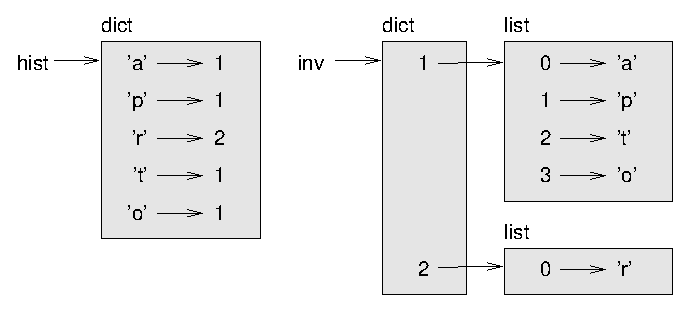
\includegraphics[scale=0.8]{figs/dict1.eps}}
\caption{状態図}
\label{fig.dict1}
\end{figure}

図\ref{fig.dict1}には辞書histとinverseの状態図を示した。
辞書は上部に変数の型を示す{\tt dict}のラベルをはり、箱の中味はキーと値のペアを要素として並べた。
もし値が整数や文字列であるときにはそれらは箱の中に並べたが、それらがリストであるときには別な箱を用意してその中に纏めて並べた。\par
リストは辞書の値として取り得るが、キーとしては使えない。以下は間違ったその例である：
\begin{verbatim}
>>> t = [1, 2, 3]
>>> d = dict()
>>> d[t] = 'oops'
Traceback (most recent call last):
  File "<stdin>", line 1, in ?
TypeError: list objects are unhashable
\end{verbatim}
既に述べたように辞書はハッシュテーブルを使って実装される。
その意味するところは、キーは{\bf ハッシュ可能（hashable）}でなければならないということだ。\par
{\bf ハッシュ（hash）}は値（任意の型の）を受け取り、整数を返す関数である。
辞書はこの整数（ハッシュ値という）をキーと値のペアの保存やルックアップに使う。\par
辞書のキーが変更不可である場合は問題ないが、
キーがリストのような変更可能なものであるといろんなことが起こる。
例えば、キーと値のペアを生成したとする。キーはハッシュされ、キーと値のペアは対応するところに保存される。
そこでキーを変更したとしよう。変更されたキーはハッシュされる。新たなハッシュ値により、キーと値のペアは別なとことに保存される。
こうなると、同一のキーに対して二つのアイテムができるとか、キーを発見できなくなるなどの混乱が起こる。\par
このため、キーはハッシュ化されなければならなく、リストのような変更可能なものであってはいけない訳である。
このような制限を回避する方法は次章で触れるタプルを使うことである。\par
辞書自体は変更可能なのでキーには使えないが、値としては使える。
%
\section{メモ}
6.7節の関数{\tt fibonacci}で引数の大きな数を与えれば与えるほど実行にかかる時間が長くなることに気が付く。
さらに大きな数では計算時間が急激に増える。
この理由を理解するために、引数{\tt n=4}で{\tt fibonacci}を実行した場合を調べてみる。
それには図\ref{fig.fibonacci}のような{\bf 呼び出しグラフ（call graph）}を作成してみるとよい。\par
呼び出しグラフは関数フレームの集合を示す。
そこでは呼びだされた関数とその関数を呼んだ関数が線で繋がれている。
グラフの頂点は引数{\tt n=4}の{\tt fibonacci}で、
これが引数{\tt n=3}と{\tt n=2}の{\tt fibinacci}を呼んでいる。
替わって、引数{\tt n=3}の{\tt fibinacciは}引数{\tt n=2}と{\tt n=1}を呼んでいる。
等々である。\par
このようなグラフから{\tt fibonacci(0)}や{\tt fibonacci(1)}が全体で呼ばれている回数を調べてみよう。
これからこの{\tt fibonacci}プログラムはこの問題の解答としては不充分であることが分かる。
この欠点は引数が大きくなるほど強調される。\par
この解決法の一つは既に計算し終えた値を辞書に保存し値の軌跡を残して置くことだ。
このように計算した結果を後のために保存することを{\bf メモ（memo）}と呼ぶ。
%
\begin{figure}[htbp]
\centerline
{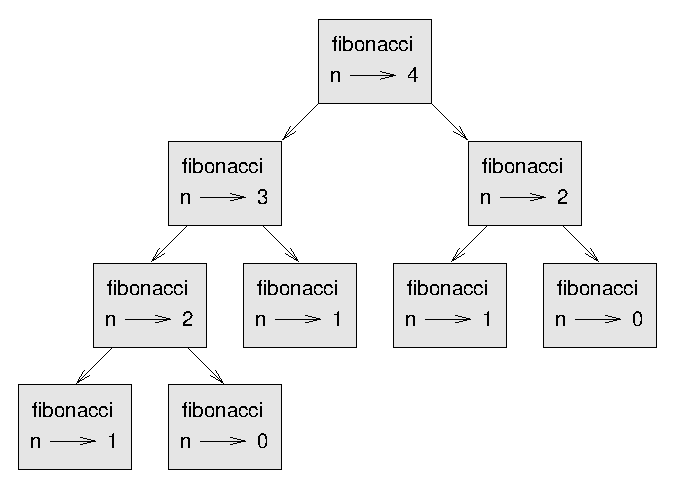
\includegraphics[scale=0.7]{figs/fibonacci.eps}}
\caption{呼び出しグラフ}
\label{fig.fibonacci}
\end{figure}

以下はそれを使った関数fibinacciの実装である：
\begin{verbatim}
known = {0:0, 1:1}

def fibonacci(n):
    if n in known:
        return known[n]
    res = fibonacci(n-1) + fibonacci(n-2)
    known[n]=res
    return res
\end{verbatim}
大域変数{\tt known}は辞書で既に計算したフィボナッチ数を保存して置く。
この辞書の初期値は0を0にマップ、1を1にマップさせるものである。
関数{\tt fibinacci}が呼ばれる度に辞書{\tt known}が検索される。結果があればそれを使う。
なければ計算してその結果を辞書に残すと共に戻り値として返す。 \
この新たな{\tt fibonacci}関数を実行してみると、さらに従来の{\tt fibinacci}関数と比較してかなり速いことを実感するはずだ。
%
\section{大域変数}
前節の例では変数{\tt known}は関数の外で生成された。
これは{\verb"__main__"}と呼ばれる特別なフレームにこの変数が属していることを意味している。
{\verb"__main__"}に属する変数は{\bf 大域変数（global variable）}と呼ばれる。
この変数は任意の関数からアクセスすることができるからだ。
関数に属するローカル変数が関数の終了と共に消失するのと異なり、大域変数は一つの関数呼ばれ、次が呼ばれようと残る。\par
大域変数としてよく使われるのがある条件が満たされたどうかを表示する{\bf フラグ（flags）}機能を担った変数だ。
以下{\tt verbose}というフラグを使い詳細表示を制御する例である：
\begin{verbatim}
verbose = True

def example1():
    if verbose:
         print('Running examle1')
\end{verbatim}
もしこの大域変数の再代入をしようとすると予想外のことが起こる。\par
以下はある関数が呼ばれたことがあるかを追跡することを意図したプログラムである。
\begin{verbatim}
been_called = False

def example2():
    been_called = True    #間違い
\end{verbatim}
このプログラムを実行すると、大域変数の値が変化していないことに気が付くはずだ。
問題は関数{\tt example2}では新たなローカル変数{\tt been\_called}が作成されたことにある。
関数が終了するとこのローカル変数は消失し、大域変数の値は何も変化はない。 \par
関数の内部で大域変数へ再代入をしたいときは使う前に大域変数の{\tt 宣言（declare）}をする：
\begin{verbatim}
been_called = False

def example2():
    global been_called
    been_called = True  
\end{verbatim} 
{\tt global}文はインタプリタに、
「この関数では、{\tt been\_called}と呼ばれるものは大域変数で、ローカル変数として生成したものでないよ」と伝える役目をしている。\par
大域変数の更新についても同様だ：
\begin{verbatim}
count = 0

def example3():
    count = count + 1  #間違い
\end{verbatim}
このまま実行すると以下のエラーが出る：
\begin{verbatim}
UnboundLocalError: local variable 'count' referenced before assignment
\end{verbatim}
Pythonは変数{\tt count}をローカルとみなし、代入の前に参照していることでエラーを吐き出す。
解決法は{\tt count}を大域変数として宣言することだ：
\begin{verbatim}
def example3():
    global count
    count += 1  
\end{verbatim} \par
大域変数が変更可能なものであると、宣言なしで変更できる：
\begin{verbatim}
known = {0:0, 1:1}

def example4()
    known[2] = 1
\end{verbatim}
従って大域リストに対しては、要素の追加、削除、変更は宣言なしでできる。しかし、再代入では宣言が必要となる：
\begin{verbatim}
def example5():
    global known
    known = dict()
\end{verbatim}
大域変数は便利なものであるが、多用しその値を頻繁に変更するとデバッグが難しくなる。
%
\section{デバッギング}
扱うデータ（データセット）の量が多くなるに従って否応なしに表示によるデバッグや手作業によるデータのチェックが必要になる。
ここではそのようなデータが多いプログラムに対するデバッグ作業のいくつかの示唆を示す： 
\begin{description}
\item[入力のスケールダウン：] もし可能なら、入力するデータ量を減らしてみる。
例えば、テキストファイルを読むプログラムであるなら、最初の10行だけ読んでみる。
または最少単位のデータを用意する。これはファイル自体を修正するか、
もっといい方法はプログラムを修正して最初の{\tt n}行だけ読むようにする。 \par
それでもエラーがあるときには、そのエラーを明らかにできる更に小さいデータ量で実行してみる。エラーが修正できたら、
データ量を徐々に多くしてみる。
\item[要約的把握や型の確認：] データセットの全てを表示し、
確認作業をする替わりに、例えば、辞書の要素の数や数のリストの総和といったデータの要約的な量を表示してみる。
また、実行時のエラーは値が正しい型でないことからくることが多々ある。このような場合は単に値の型を表示してみることで済む場合がある。
\item[自己点検の書き込み：] 自己点検できるような機能をコードに書き込むことができる。
例えば、数値のリストの要素の平均値を計算しているとしよう。この平均値はこのリストの最大要素の値より小さいはずであり、
最小要素の値より大きいはずである。このような検証は結果が「不健全」であることを検出するから、「健全性の検証」と呼ばれている。\par
二つの異なった方法で得られた結果を比較するという検証はそれらが一貫しているかどうかの検証になる。これは「一貫性の検証」と呼ばれている。
\item[出力を綺麗に表示：] デバッグのための表示を綺麗に表示することはエラーの個所を特定することに役に立つ。
その例を6.9節でみた。モジュール{\tt pprint}の{\tt pprint}関数は組み込み型をより人間に読みやすい形式で表示する。
（{\tt pprint}は``pretty print"の略称である。）
\end{description}
足場建設のために費やした時間はデバッギングで消費する時間を縮めることができるのだ。
%
\section{語句}
\begin{description}

\item[写像（mapping）：] 一つ集合の各要素がもう一つの集合の要素に対応している関係。
%\index{mapping}

\item[辞書（dictionary）：] キーの集合から対応する値への写像。 
%\index{dictionary}

\item[キーと値のペア（keys-value pair）：] キーから値への写像に具体的な表現。
%\index{key-value pair}

\item[アイテム（item）：] 辞書におけるキーと値のペアの別名。
%\index{item!dictionary}

\item[キー（keys）：] 辞書のキーと値のペアにおいて対の最初に現れるオブジェクト。
%\index{key}

\item[値（values）：] 辞書のキーと値のペアにおいて対の二番目に現れるオブジェクト。これはこれまで
使っていた「値」よりもっと特定の状況での「値」の使い方である。
\index{value}

\item[実装（implementation）：] 計算の実際の実行方法。
%\index{implementation}

\item[ハッシュ表（hashtable）：] Pythonの辞書を実装するためのアルゴリズム。
%\index{hashtable}

\item[ハッシュ（hash）：] キーの場所を計算するためにハッシュ表を用いること。
%\index{hash function}

\item[ハッシュ可能（hashable）：] ハッシュ関数を持つデータ型。整数、浮動小数点型そして文字列のような変更不可の型はハッシュ可能であり、
リストや辞書はそうでない。
%\index{hashable}

\item[ルックアップ（look up）：] 一つキーを受け取りそれに対応する値を探すという辞書における操作。.
%\index{lookup}

\item[逆ルックアップ（reverse lookup）：] 一つの値を受け取りその値にマップしている一つまたはそれ以上のキーを探すという
辞書の操作。
%\index{reverse lookup, dictionary}

\item[シングルトン（singleton）：] 一つの要素のみを含むリスト（または他の配列）。
%\index{singleton}

\item[呼び出しグラフ（call graph）：] 一つのプログラムの実行過程で生成される各フレームで関数の呼び出し側と呼ばれた関数側とを
矢印で結ぶグラフ表現。
%\index{call graph}
%\index{diagram!call graph}

\item[メモ（memo）：] 余計な計算を回避するために計算を終えた結果を保存して将来に備える。
%\index{memo}

\item[大域変数（global variable）：:] 関数の外で定義される変数。その変数は他の関数からもアクセスできる。
%\index{global variable}

\item[フラグ（flags）：] 条件が満たされているかどうかを表示するために用いられるブーリアン変数。
%\index{flag}

\item[宣言（declare）：] {\tt global}のように変数の属性をインタプリタに知らせる文。
%\index{declaration}

\end{description}
%
\section{練習問題}
\noindent
{\bf 練習問題\tp.1} ファイル{\tt words.txt}を読み込み、英単語をキーとする辞書を作成せよ。
値を何にするかは問わない。そして演算子{\tt in}を使ってある文字列がその辞書にあるかどうかを調べる関数を作成せよ。\par
もし練習問題10.10をやっていれば、二分探索とリストに対する演算子{\tt in}の実装の違いによる検索スピードを比較できる。\\

\noindent
{\bf 練習問題\tp.2} 辞書にたいするメソッド{\tt setdefaut}のドキュメンテーションを読み、関数{\tt invert\_dict}をコンパクトに書け。\\
解答例：\url{https://thinkpython.com/code/invert_dict.py}.\\

\noindent
{\bf 練習問題\tp.3} 練習問題6.2で扱った{\tt Ackermann}関数に対してメモ機能を付けたものせよ。
そして、このメモ機能があると大きな値の引数でも関数の評価が可能かどうかを確認せよ。
ヒント：なし。\\
解答例：\url{https://thinkpython.com/code/ackermann_memo.py}.\\

\noindent
{\bf 練習問題\tp.4} 練習問題10.7ではリストを引数として受け取り
そのリストの要素が重複しているときは{\tt True}を返す関数{\tt has\_duplicates}を作った。
辞書を利用してより高速でコンパクトな改訂版関数{\tt has\_duplicates}を作成せよ。 \\
解答例：\url{https://thinkpython.com/code/has_duplicates.py}\\

\noindent
{\bf 練習問題\tp.5} 二つの単語は一つを回転したら他方に一致するときこの二つの単語は「回転ペア」と呼ぶことにする。
{\tt words.txt}を読み込んで全ての「回転ペア」検出するプログラムを作成せよ（練習問題8.5の関数{\tt rotate\_word}を参照せよ）。\\
解答例：\url{https://thinkpython.com/code/rotate_pairs.py} \\

\noindent
{\bf 練習問題\tp.6} これもCarTalkのパズル名人から借用した。　\\
(\url{http://www.cartalk.com/content/puzzlers}) \\
Dan O'learyという人物から送られてきたものだ。
\begin{quote}
五文字からなる一音節の単語を思いついたが以下のような面白い性質を持っているというのだ。
まず、先頭の文字を削除すると四文字の単語になるがこれが元の単語と同音異義語である。
つまりこの二つの単語の発音は厳密に一致するのだ。さらに、この文字を元のところにもどして、
二番目の文字を削除すると四文字の単語になるが、これも元の単語の同音異義語になる。
問題は、この元の単語はなにかだ。\par
さて、成り立たないが例を示す。単語{\tt wrack}つまり{\tt W-R-A-C-K}を例にとろう。この単語は``wrack with pain"（痛さに卒倒する）などに使う言葉だ。先頭の一文字を削除すると{\tt R-A-C-K}になる。
``Holy cow, did you see the rack on that buck! It must have been a nine pointer!"（おやまあ、あの雄ジカの角を見たかい。あれはナインポインタに違いないよ）などにみるね。
そしてこの言葉は完全な同音異義語である。さて、{\tt 'w'}を元に戻し、
二番目の文字を削除すると、``wack"が得られる。これも実在する単語であるが、この言葉は前二者と同音異義語になっていない。\par
しかし、Danやわれわれが知っている単語で少なくとも一つは条件を満たす単語がある。その単語は何か？
\end{quote}
ある文字列が単語リストにあるかどうかを調べる目的で練習問題11.1の辞書を使うことができる。
二つの単語は同音異義語であるかどうかの検定にはCMU発音辞典を使うことができる：
\url{http://www.speech.cs.cmu.edu/cgi-bin/cmudict}または 
\url{https://thinkpython.com/code/c06d}からダウンロードできる。
また、\url{https://thinkpython.com/code/pronounce.py}をダウインロードできる。
この中の{\tt read\_dictionary}は発音辞典から単語とその単語の主要な発音をPythonの辞書として戻す関数である。\par
パズル名人のこの問題を解くプログラムを作成せよ。\\
解答例：\url{https://thinkpython.com/code/homophone.py}
%
\chapter{タプル}
この章ではさらにもう一つの組み込み型であるタプルを取り上げ、その後リスト、辞書そしてタプルが
如何に相互に働くかを見ることにする。また可変長引数リスト、「纏める」そして「ばらす」といった操作
の有益な特徴にも触れる。\par
閑話休題：``tuple"をどう発音するか一致して見解はない。``supple"と韻が同じように``tuhple"
と発音する人たちがいる。一方プログラミングの中身を踏まえて多くの人たちは``quadruple"と
韻が同じで``too-ple"と発音する。
%
\section{タプルは変更不可}
{\bf タプル（tuple）}は値の配列である。その値は任意の型でよい。
また、整数でインデックス化されている。これらの点で、タプルはリストに似ている。
大きな相異は、タプルは変更不可なことである。
構文的にはタプルは値をカンマで区切った配列である：
\begin{verbatim}
>>> t = 'a', 'b', 'c', 'd', 'e'
\end{verbatim}
必ずしも必要でないが、タプルを括弧で括ることが普通である：
\begin{verbatim}
>>> t = ('a', 'b', 'c', 'd', 'e')
\end{verbatim} \par
一つの要素だけでタプルを生成するときには最後にカンマが必要だ：
\begin{verbatim}
>>> t1 = 'a',
>>> type(t1)
<class 'tuple'>
\end{verbatim}
値を括弧で括ったものはタプルではない：
\begin{verbatim}
>>> t2 = ('a')
>>> type(t2)
<class 'str'>
\end{verbatim} \par
組み込み関数{\tt tuple}を使って空のタプルを作ることができる。引数なしでそれを使う：
\begin{verbatim}
>>> t = tuple()
>>> t
()
\end{verbatim} \par
もしも引数が配列（文字列、リスト、タプル）であるとすると、結果はその配列要素を要素とするタプルが得られる：
\begin{verbatim}
>>> t = tuple('lupins')
>>> t
('l', 'u', 'p', 'i', 'n', 's')
\end{verbatim}
組み込み関数名tupleを変数として使うことは避けるべきである。\par
リストに対して使った演算はタプルで有効だ。角括弧は要素のインデックスとして使える：
\begin{verbatim}
>>> t = ('a', 'b', 'c', 'd', 'e')
>>> t[0]
a
\end{verbatim}
スライス演算も区間要素を選択するのに使える：
\begin{verbatim}
>>> t[1:3]
('b', 'c')
\end{verbatim}
しかし、タプルの要素を変更することはできない：
\begin{verbatim}
>>> t[0] = 'A'
TypeError: object doesn't support item assignment
\end{verbatim}
しかし別なタプルに置き換えることはできる：
\begin{verbatim}
>>> t = ('A',) + t[1:]
>>> t
('A', 'b', 'c', 'd', 'e')
\end{verbatim}
つまりこの文は新規にタプルを作り変数{\tt t}にそれを参照させている。\par
比較演算子はタプルを初めてとしてリストにも適用できる。
Pythonは初めの要素を比較する。
等しいならば次ぎの要素を比較する。異なる要素に出会うまでこれを繰り返す。
ここでの比較が結果である。だから以降の要素は無視される。
\begin{verbatim}
>>> (0, 1, 2) < (0, 3, 4)
True
>>> (0, 1, 2000000) < (0, 3, 4)
True
\end{verbatim} 
%
\section{タプルの代入}
二つの変数の交換は有用なことが多々ある。伝統的な手法は一時的な変数を使うものである。
変数{\tt a}と{\tt b}の交換を例にみよう：
\begin{verbatim}
>>>temp = a
>>>a = b
>>>b = temp
\end{verbatim}
{\bf タプルの代入（tuple assignment）}はもっとエレガントが手法を提供している：
\begin{verbatim}
>>>a, b = b, a
\end{verbatim}
左辺は変数のタプルであり、右辺は表式のタプルである。各要素が対応する変数に代入される。
右辺の表式は代入する前に評価される。\par
左辺の変数の個数は右辺の値の個数と一致している必要がある。
\begin{verbatim}
>>> a, b = 1, 2, 3
ValueError: too many values to unpack
\end{verbatim} \par
もっと一般的には、右辺は任意に配列（文字列、リスト、タプル）でもよい。
電子メールアドレスをユーザ名とドメイン名に{\tt split}を用いて分離する例を示す：
\begin{verbatim}
>>> addr = 'monty@python.org'
>>> uname, domain = addr.split('@')
\end{verbatim}
右辺は二つの要素を持つリストであり、
先頭の要素は{\tt uname}に代入され、二番目は{\tt domain}に代入される。
\begin{verbatim}
>>> uname
monty
>>> domain
python.org
\end{verbatim}
%
\section{タプルを戻り値}
厳密にいうと関数の戻り値は一つの値のみであるが、それがタプルであると多数の値を戻り値にする効果がある。\par
例を示す。二つの整数のわり算で商と余りを出す問題を考えよう。
組み込み関数{\tt divmod}を使うと二つ整数のわり算の商と余りをタプルとして戻してくれる。　
だから、この二つをタプルに代入することができる。
\begin{verbatim}
>>> t = divmod(7, 3)
>>> t
(2, 1)
\end{verbatim}
または要素毎の代入でもよい：
\begin{verbatim}
>>> quot, rem = divmod(7, 3)
>>> quot
2
>>> rem
1
\end{verbatim} \par
以下は簡単な例である：
\begin{verbatim}
def min_max(t):
    return min(t), max(t)
\end{verbatim}
{\tt min}、{\tt max}は配列の最大と最小の要素を見つける組み込み関数である。
関数{\tt min\_max}はその両方を計算し、それを一つのタプルとして戻している。
%
\section{可変長引数タプル}
関数は可変長引数を受け取りことができる。
記号{\tt *}で始まる仮引数は複数の引数を一つのタプルに{\bf 纏める（gathers）}。
例えば、関数{\tt print\_all}は任意の数の引数を受け取り、それらを{\tt print}する：
\begin{verbatim}
def print_all(*args):
    print(args)
\end{verbatim}
纏め引数の名前は自由に取れるが伝統的に{\tt arg}を使う。この関数が正確に動くことを確かめる：
\begin{verbatim}
>>> print_all(1, 2.0, '3')
(1, 2.0, '3')
\end{verbatim} \par
「纏める」の補語は{\bf ばらす（scatter）}である。
値の配列があり、それを複数の引数を受け取る関数に通したいときは、記号{\tt *}を使う。
例として、{\tt divmod}関数は厳密に二つの引数を要求するので、一つのタプルではエラーになる：
\begin{verbatim}
>>> t = (7, 3)
>>> divmod(t)
TypeError: divmod expected 2 arguments, got 1
\end{verbatim}
しかし、タプルをばらすと二つの引数になり正常に動く：
\begin{verbatim}
>>> divmod(*t)
(2, 1)
\end{verbatim} \par
組み込み関数の多くは可変長引数タプルを使っている。
例を挙げれば、{\tt min}、{\tt max}も任意の長さの引数を受け取ることができる。
\begin{verbatim}
>>> max(1, 2, 3)
3
\end{verbatim}
しかし、関数sumはそうでない。
\begin{verbatim}
>>> sum(1, 2, 3)
TypeError: sum expected at most 2 arguments, got 3
\end{verbatim}
（訳注：関数{\tt sum}は配列を受け取りその要素の和を戻す。）\par
そこで任意の引数を受け取り、その総計を返す関数{\tt sum\_all}を作成せよ。
%
\section{リストとタプル}
組み込み関数{\tt zip}は引数として二つ以上の配列を受け取り、
それらの配列の各要素を一つずつ組みにして「纏めて」タプルとし、それらのリストを返す。
この関数の名前は二つの歯を交互に組み合わせるジッパーに由来している。
\begin{verbatim}
>>> s = 'abc'
>>> t = [0, 1, 2]
>>> zip(s, t)
<zip object at 0x7f7d0a9e7c48>
\end{verbatim}
結果は値のペアを繰り返し処理することに特化した{\bf ジッパーオブジェクト（zip object）}である。
最も一般的な{\tt zip}の使い方は{\tt for}ループの中の{\tt in}演算子によるものである：
\begin{verbatim}
>>> for pair in zip(s, t):
...     print(pair)
...
('a', 0)
('b', 1)
('c', 2)
\end{verbatim}
ジッパーオブジェクトは配列を横断的に繰り返す{\bf イテレータ（iterator）}の一種である。イテレータは
ある面でリストに似ているが、リストと異なり、イテレータの要素を選択するときインデッススは使えない。\par
もしもリストの演算やメソッドを使いたいのであれば、ジッパーオブジェクトをリストにするとよい：
\begin{verbatim}
>>> list(zip(s, t))
[('a', 0), ('b', 1), ('c', 2)]
\end{verbatim}　
\indent
ジッパーオブジェクトを生成するとき、もし二つの配列の長さが一致しないときは短い方に合わせる：
\begin{verbatim}
>>> list(zip('Anne', 'Elk'))
[('A', 'E'), ('n', 'l'), ('n', 'k')]
\end{verbatim}　
\indent
このようなタプルを要素とするリストに対してはリストの{\tt for}を使った横断的な処理ではタプルへの代入を使うことができる：
\begin{verbatim}
>>> t = [('a', 0), ('b', 1), ('c', 2)]
>>> for letter, number in t:
	print(letter, number)
\end{verbatim}
ループは回る度にPythonはタプルを選択し、そのタプルの要素を{\tt letter}と{\tt number}に代入する。結果は以下のようになる：
\begin{verbatim}
a 0
b 1
c 2
\end{verbatim}
これら関数zip, for文, そしてタプルの代入を使うと二つ以上の配列を一時に横断的調べることができる仕掛けが作れる。
関数{\tt has\_match}を例に示す。この関数は二つの配列の同じインデックスの要素が少なくとも一つは一致するかどうかを調べるものである。
\begin{verbatim}
def has_match(t1, t2):
    for x, y in zip(t1,t2):
        if x == y:
            return True
    return False
\end{verbatim} 
\indent
配列を横断的に眺めると同時にその要素のインデックスも必要なときには、関数{\tt enumerate}を使うとよい：
\begin{verbatim}
for index, element in enumerate('abc'):
    print index, element
\end{verbatim}
このループの表示は以下のようになる：
\begin{verbatim}
0 a
1 b
2 c
\end{verbatim}
%
\section{辞書とタプル}
辞書には{\tt items}というメソッドがある。これは辞書のキー・値ペアをタプルとしたリストを返す関数である。
\begin{verbatim}
>>> d = {'a':0, 'b':1, 'c':2}
>>> t = d.items()
>>> t
dict_items([('c', 2), ('a', 0), ('b', 1)])
\end{verbatim}
結果は{\tt dict\_items}オブジェクトで、キーと値のペアを繰り返し処理するイテレータである。このオブジェクトは以下のように
{\tt for}文のなかで{\tt in}演算子を使う：
\begin{verbatim}
>>> for key, value in d.items():
...     print(key, value)
...
c 2
a 0
b 1
\end{verbatim}
辞書で予想できたように並びは順不同である。 \par
逆方向の操作もある。タプルのリストを新規辞書に変換する：
\begin{verbatim}
>>> t = [('a', 0), ('c', 2), ('b', 1)]
>>> d = dict(t)
>>> d
{'a': 0, 'c': 2, 'b': 1}
\end{verbatim} 
\indent
この関数{\tt dict}と関数{\tt zip}を組み合わせると大変簡明な辞書生成の方法ができあがる：
\begin{verbatim}
>>> d = dict(zip('abc',range(3)))
>>> print d
{'a': 0, 'c': 2, 'b': 1}
\end{verbatim} 
\indent
辞書のメッソド{\tt update}はタプルのリストを受け取り既存の辞書に追加する。\par
タプルを辞書のキー（リストはこの目的には使えないので）に使うことがよくある方法である。
例えば、ファーストネームとラストネームを対にして辞書のキーとして使い、電話番号を値とする辞書である。
それらを{\tt first},{\tt last},{\tt number}とすると以下のように書くことができる：
\begin{verbatim}
dictionary[last,first] = number
\end{verbatim}
角括弧内の表式はタプルである。このような辞書の横断的な処理にもタプルの代入が使える。
\begin{verbatim}
for last, first in dictionary:
    print first, last, dictionary[last, first]
\end{verbatim}
このループはタプルであるキーを横断的に眺める。
各タプルの組みを{\tt last},{\tt first}に代入し、それに対応する辞書の値を{\tt print}する。\par
 
\begin{figure}[htbp]
\centerline
{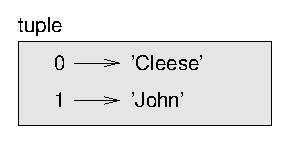
\includegraphics[scale=0.8]{figs/tuple1.eps}}
\caption{状態図}
\label{fig.tuple1}
\end{figure}
%
\begin{figure}[htbp]
\centerline
{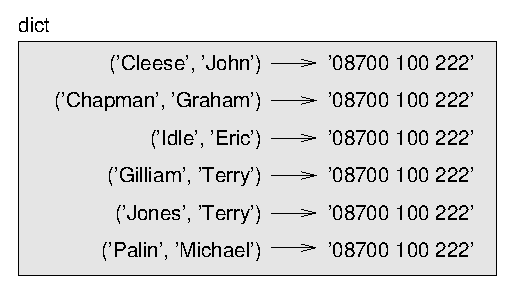
\includegraphics[scale=0.8]{figs/dict2.eps}}
\caption{状態図}
\label{fig.dict2}
\end{figure}
%
この辞書のキーのタプルに対する状態図を描く方法には二つある。詳しい版ではリストと同じようにインデックスとそれが示す要素を書く。
例として、{\tt (Cleese, John)}のタプルを図\ref{fig.tuple1}に示した。もっと大きな図ではそのような細部は無くてもよいと思うだろう。
電話帳の例を図\ref{fig.dict2}に示した。そこではPythonで使うタプルの表式そのものを使った。
対応する電話番号はBBCの苦情窓口のものだ。電話しないでほしい。
%
\section{配列の配列}
ここまではタプルのリストの話を進めてきたが、これらはリストのリスト、タプルのタプル、リストのタプルなどにも大凡適用できる。
重複を避けるために配列の配列として話を纏めることにする。\par
多くの状況で、異なった形式の配列（文字列、リスト、タプル）は相互に交換可能である。
それではどのようにして、何故に他の形式より、ある配列形式を好ましいとして選択すべきだろうか？\par
自明なことであるが、文字列は要素が文字のみであるということから他の形式の配列より制限がきつい。
それらは変更不可でもある。もし文字の一部を変更したいと思ったら、文字列の替わりに文字のリストを使うに違いない。\par
リストは変更可能ということから、タプルより一般的と言える。しかし、タプルの方が好ましいと思われるいくつかの場合がある：
\begin{enumerate}
\item 例えば{\tt return}文のようないくつかの状況では、リストよりタプルで処理する方が構文的に簡単になることがある。
その他の状況ではリストが好ましいかもしれない。
\item もし配列を辞書のキーとして使いたいなら、変更不可のタプルや文字列を使わざるをえない。
\item もし配列を関数の引数に渡したい場合があるなら、リストによる別名処理の弊害を避けるためにタプルを使った方が安全だ。
\end{enumerate}
タプルは変更不可なので、既存のリストの変更を伴う{\tt sort}や{\tt reverse}などのメソッドは存在しない。
しかし、{\tt sorted}や{\tt reversed}などの関数が用意されていて任意の配列を受け取り新しい配列を返すことができる。
%
\section{デバッギング}
リスト、辞書、タプルは一般に{\tt データ構造（data structure）}として知られているが、
この章ではタプルのリスト、タプルをキーとしてリストを値とする辞書のような複合データ構造を初めてとりあげた。
複合データ構造は有用だが、私が{\bf 型エラー（shape errors）}と名付けたエラーに陥りやすい。
このエラーはデータ構造の間違った型や大きさ、複合の仕方が原因として起きる。\par
例えば、一つの整数を要素とするリストを期待していたのに、普通の整数が与えられたとすると、動かなくなるといったものだ。
この種のエラーをデバッグするために、{\tt structshape}というモジュールを作り、関数{\tt structshape}が使えるようにした。
この関数は任意のデータ構造を引数として受け取りその型について纏めた文字列を返す関数である。
ダウンロード先は\url{https://thinkpython.com/code/structshape.py}である。\par
以下いくつかの簡単な例を示す：
\begin{verbatim}
>>> from structshape import structshape
>>> t = [1,2,3]
>>> structshape(t)
list of 3 int
\end{verbatim}
もっと凝ったプログラムでは``list of 3 ints"と書くかもしれない。しかし、複数形を斟酌しない方が簡単だ。\\
リストのリストだと以下のようになる：
\begin{verbatim}
>>> t2 = [[1,2], [3,4], [5,6]]
>>> structshape(t2)
list of 3 list of 2 int
\end{verbatim}
もしも要素が異なった型であるとすると、{\tt structshape}は型毎に纏めて表示する：
\begin{verbatim}
>>> t3 = [1,2,3,4.0,'5','6',[7],[8],9]
>>> structshape(t3)
list of (3 int, float, 2 str, 2 list of int, int)
\end{verbatim}
タプルのリストでは：
\begin{verbatim}
>>> a = 'abc'
>>> lt = zip(t,a)
>>> structshape(lt)
list of 3 tuple of (int, str)
\end{verbatim}
整数をキーとして文字列を値とする三つの要素を持つ辞書では
\begin{verbatim}
>>> d = dict(lt)
>>> structshape(d)
dict of 3 int->str
\end{verbatim}
データ構造の追跡で何か問題が起きたら、この関数{\tt structshape}が有効だ。
%
\section{語句}
\begin{description}

\item[タプル（tuple）：] 要素を変更できない配列。
%\index{tuple}

\item[タプルの代入（tuple assignment）：] 右側に一つの配列、左側に複数の変数のタプルを置く代入文。
右側が評価され対応する要素（複数の値からなる）が左側のタプルに代入される。
%\index{tuple assignment}
%\index{assignment!tuple}

\item[纏める（gathers）：] 可変長引数タプルを纏める操作。
%\index{gather}

\item[ばらす（scatter）：] 関数の引数（複数）を一つの配列として扱う操作。
%\index{scatter}

\item[ジッパーオブジェクト（zip object）：] 組み込み関数{\tt zip}によって生成されるオブジェクトで
タプルを要素とする配列の形式をとり繰り返し処理に特化したオブジェクト。
%\index{zip object}

\item[イテレータ（iterator）：] 配列の形式をとり繰り返し処理に特化したオブジェクト、しかし
リストに対する演算やメソッドは持っていない。
%\index{iterator}

\item[データ構造（data structure）：] リスト、辞書、そしてタプル等のかたちに纏められた値の集合。
%\index{data structure}

\item[型エラー（shape errors）：] データ構造のような複雑に纏められたデータにアクセスする際に起こる型の不一致によるエラー。
%\index{shape}

\end{description}
%
\section{練習問題}
\noindent
{\bf 練習問題\tp.1} 文字列を受け取りその文字列に含まれている文字の頻度を降順に表示する
プログラム{\tt most\_frequent}を作成せよ。
色々な言語で書かれた文書を調べ文字の頻度分布が言語でどのように異なるかを調べ、以下の文献と比較せよ：\\
\url{http://en.wikipedia.org/wiki/Letter_frequencies}。\\
解答例：\url{https://thinkpython.com/code/most_frequent.py} \\
\noindent
{\bf 練習問題\tp.2} アナグラム再論！
\begin{enumerate}
\item ファイルから単語集を読み込み（9.1節をみよ）、アナグラムになっている単語の全てを表示するプログラムを作成せよ。\\
どんな出力になるのかを例で示す：
\begin{verbatim}
['deltas', 'desalt', lasted', 'salted', 'slated', 'staled']
['retainers', 'ternaries']
['generating', 'greatening']
['resmelts', 'smelters', 'termless']
\end{verbatim}
ヒント：文字のセットとそれらの文字から作れる単語のリストとを写像する辞書を作ることになるかもしれない。
問題はいかに文字のセットをキーとする辞書を作るかである。
\item 前のプログラムを修正して最大の数の単語を含むアナグラムを最初に表示し、次ぎは二番目というような順序に表示にせよ。
\item スクランブル（単語ゲーム）では、ボード上にある一文字とラックに用意された七個の
文字タイルを全て使って八文字の長さの単語が作れると「ビンゴ」になる。どんな八文字のセットが最も「ビンゴ」になりやすいか？
\end{enumerate}
ヒント：七つの単語が作れるものがある。 \\
解答例：\url{https://thinkpython.com/code/anagram_sets.py} \\

\noindent
{\bf 練習問題\tp.3} 一つ単語の中にある二文字を入れ替えると他の単語になるときこの二つの単語は「字位転換ペア（metathesis）」という。
辞書中の全ての字位転換ペアを見つけ表示するプログラムを作成せよ。\\
ヒント：単語集の全てのペアを検証するな、そして、一つの単語の可能な交換の全てを検証するな。
（訳注：その心は含まれて文字が同じもののみ、つまりアナグラムになっていて二個所で文字が異なる単語だ）。\\
解答例：\url{https://thinkpython.com/code/metathesis.py} \\
出典：この練習問題は以下の例題に啓発された：\url{http://puzzlers.org} \\

\noindent
{\bf 練習問題\tp.4} これもCar Talkのパズル名人の問題である。
（\url{http://www.cartalk.com/content/puzzlers}） \\
\begin{quote}
英単語があり、それを構成している文字を一回に一文字を削除して文字を詰めると新たな単語になるような最も長い単語はなにか？
さて、文字の削除は先頭でも中程でもよいが、文字の並び替えはできない。
文字を削除したら単に文字を詰めてみると他の英単語になっている。
これが成功したら、その新しい単語から一文字削除し、詰めると英単語が現れる。
最後は一文字だけになるがこれも辞書にある英単語である。
このような英単語の中で最も長い単語はなにか、また何文字からなるか？これが知りたいことである。
\end{quote}
平凡で短い単語spriteで例を示す。spriteで始める。
まず、文字rをとる、するとspiteが作られる。さらに、文字eをとると、spitができる。
またさらに、文字sをとると、pitが生成され、文字pをとるとitが、さらに文字tをとるとIが出現する。
最後のIも辞書にある単語だ。\par
上の例のように最終的に一文字の英単語に縮小できる（全縮小可能と呼ぶ）全ての英単語を見つけるプログラムを作成せよ、
そして、その中で最も長い単語をみつけよ。
この練習問題は今までのものより難しいので、いくつか示唆を与えておこう。
\begin{enumerate}
\item 単語を引数として受け取り、それから一文字削除してできる単語（子ども）の全てをリストにして返す関数を生成してみる。
\item ある単語はもしその子どもの一つでも全縮小可能ならば再帰的に全縮小可能である。そこでは空の文字列を再帰の基底ケースと考える。
\item 今まで使ってきた{\tt words.txt}には一文字の単語が含まれていないので、``I"、``a"と空文字をそれに加える。
\item プログラムの効率を高めるために全縮小可能単語を記憶しておくことが考えられる。
\end{enumerate} 
\noindent
解答例：\url{https://thinkpython.com/code/reducible.py}.
%
\chapter{事例研究：データ構造・選択}
この時点まででPythonの中核になるデータ構造を学んだことになり、そしてそれらを使う上で有用な幾つかのアルゴリズムを
学習した。もしもあなたが更にアルゴリズムについて深く学びたいのであれば、付録Bを読んでみるよい機会かもしれない。
しかしこれからの議論の前にそれを読まなければならないというわけではない。それはあなたが興味を持ったときに
読めばよい。\par
この章ではデータ構造の選択やそれらの使い方を考える練習問題を伴なった事例研究を取り上げる。
%
\section{単語頻度分布解析}
いつものように解答例をみる前に、少なくとも解答を試みるようにしてほしい。 \\

\noindent
{\bf 練習問題\tp.1} ファイルからテキストを読み、単語に分解し、区切り文字や句読点を取り除き
且つ大文字を全て小文字に変換するプログラムを作成せよ。 \\
ヒント：モジュール{\tt string}は空白、タブ、
改行文字等を含む文字の定義{\tt whitespace}や句読点を集めた文字の定義{\tt punctuation}を提供している。確かめてみよう：
\begin{verbatim}
>>> import string
>>> print string.punctuation
!"#$%&'()*+,-./:;<=>?@[\]^_`{|}~ 
\end{verbatim} 
さらに、文字列に対するメソッド{\tt strip}, {\tt replace}, {\tt translate}なども使える。\\

\noindent
{\bf 練習問題\tp.2} グーテンベルグ・プロジェクト（\url{http://gutenberg.org}）から好みの本を
テキストベースでダウンロードしてPythonで読めるようにせよ。
そして、使われている単語を表示してみる。異なった時代、異なった著者の異なった著書で得られた結果を比較せよ。
どの著者が最も多くの語彙を使っているか？\\

\noindent
{\bf 練習問題\tp.3} 前の練習問題を修正して取りあげた本で使われている最頻度度二十番目までの単語を表示せよ。\\

\noindent
{\bf 練習問題\tp.4} 第9.1節の単語集（words.txt）を読み込み、取りあげた本で使っている単語でこの単語集にないものを表示せよ。
誤植はいくつあるか？単語集に掲載すべき通常の単語はいくつあるか？はっきりしないものはいくつあるか？
%
\section{乱数}
ある与えられた入力に対してコンピュータプログラムは常に同一の結果を出力する。
この状況を{\bf 決定論的（deterministic）}と呼ぶ。われわれは常にこのような状況を期待しているので、
決定論的な処理は良好だと思っている。しかし、ある種のアプリケーションではコンピュータに予測不可な振る舞いを期待する。
ゲームはその明白な例であるがそれ以外にもある。 \par
プログラムで真に非決定論的な振る舞いを実現することは易しくないが、
非決定論的な振る舞いにみえるものを作るには方法がある。
その一つが{\bf 疑似乱数（pseudorandom number）}を生成するアルゴリズムである。
決定論的なプロセスで生成されるので、疑似乱数は真の意味では乱数ではないが、みた目には殆ど乱数と区別することは不可能だ。 \par
モジュール{\tt random}は疑似乱数を生成する関数を提供している（これ以降単に「乱数」と呼ぶことにする）。
関数{\tt random}は区間{\tt 0.0}から{\tt 1.0}までの間の乱数（{\tt 0.0}は含み{\tt 1.0}は含まない）を生成する。
関数randomを呼び出す毎に長い数列の中の次ぎの数が得られる。例をみるために以下を実行してみよう：
\begin{verbatim}
import random
for I in range(10):
    x = random.random()
    print(x)
\end{verbatim} 
\indent
関数{\tt randint}は二つの引数lowとhighを受け取り、このlowとhigh（両方とも含む）の区間の整数乱数を生成する：
\begin{verbatim}
>>> random.randint(5, 10)
5
>>> random.randint(5, 10)
9
\end{verbatim} 
配列の要素を乱雑の選択するのであれば関数{\tt choice}が使える：
\begin{verbatim}
>>> t = [1, 2, 3]
>>> random.choice(t)
2
>>> random.choice(t)
3
\end{verbatim}
\indent
モジュールrandomはガウス分布、指数分布、ガンマ分布などの連続分布関数に従って乱数を生成する関数を提供している。\\

\noindent
{\bf 練習問題\tp.5} 第11.2節で定義された頻度分布を引数として受け取り、
その頻度分布に従って値を選択し、その値を戻り値とする関数{\tt choose\_from\_hist}を作成せよ。
例を示す：
\begin{verbatim}
>>> t = ['a', 'a', 'b']
>>> hist = histogram(t)
>>> print(hist)
{'a':2, 'b':1}
\end{verbatim}
従ってこの関数は{\tt 'a'}を2/3の確率、{\tt 'b'}を1/3の確率で選択しなければならない。
%
\section{単語ヒストグラム}
前節の演習問題は自分で解答を試みてほしいが、解答例は以下にある。\\
\url{https://thinkpython.com/code/analyze_book1.py} \\
この解答例で使った文献も必要だ（\url{https://thinkpython.com/code/emma.txt}.）。 \par
以下はファイルから読み込んだ文献中の単語のヒストグラムを作成するプログラムである：
\begin{verbatim}
import string

def process_file(filename):
    hist = dict()
    fp = open(filename)
    for line in fp:
        process_line(line, hist)
    return hist

def process_line(line, hist):
    line = line.replace('-',' ')
    for word in line.split():
        word = word.strip(string.punctuation+string.whitespace)
        word = word.lower()
        hist[word] = hist.get(word, 0) + 1

hist = process_file('emma.txt')
\end{verbatim}
このプログラムではJane Austen著``Emma"をプレーンテキストにしたファイルemma.txtを読み込む。
関数{\tt process\_file}中のループはファイルから一行読みその都度それを関数{\tt process\_line}に渡している。
変数{\tt hist}は加算機の役割をしている。
関数{\tt process\_line}では{\tt split}を用いて単語に分解する前に
{\tt replace}を用いて一行の文字列中に含まれるハイフンを空白に置き換えている（訳注：これは合成語の処理。ハイフネーションに対しては別の処理が必要）。
その後に、単語のリストを{\tt strip}で句読点を削除、{\tt lower}で全ての文字を小文字に変換する処理を横断的に行っている
（文字列が「変換された」というのは速断である。文字列は変更不可である、だから{\tt strip}や{\tt lower}では新たな文字列が生成されたのだ）。
最後に{\tt process\_line}は新たなアイテムを追加または既存のアイテムの値を{\tt １}増加するかして更新処理をする。 \par
ファイル中の単語の総数は辞書の頻度の総和を求めることである：
\begin{verbatim}
def total_words(hist):
    return sum(hist.values())
\end{verbatim}
異なった単語の総数は辞書の中のアイテムの数である：
\begin{verbatim}
def different_words(hist):
    return len(hist)
\end{verbatim}
結果の表示の一例を以下に示す：
\begin{verbatim}
print('Total number of words:', total_words(hist))
print('Number of different words:', different_words(hist))
\end{verbatim}
結果は：
\begin{verbatim}
Total number of words: 161080
Number of different words: 7214
\end{verbatim}
%
\section{頻度の高い単語}
頻度の高い単語を検出するためには、単語とその頻度をタプルとするリストを作り、それをソートする。
関数{\tt most\_common}はヒストグラムを引数として受け取り、頻度で降順にソートし、頻度と単語をタプルとするリストを返す。
\begin{verbatim}
def most_common(hist):
    t = []
    for key, value in hist.items():
        t.append((value, key))
    t.sort(reverse=True)
    return t  
\end{verbatim}
各タプルで頻度が最初にきているので、ソートはこの頻度でソートされることになる。\par
降順にソートされているので先頭の十個のアイテムを表示してみる：
\begin{verbatim}
t = most_common(hist)
print('The most common words are:')
for freq, word in t[:10]:
    print(word, freq, sep='\t') #'\t'はタブ
\end{verbatim}
Emmaを解析した結果は以下のようになる：
\begin{verbatim}
The most common words are:
to      5242
the     5205
and     4897
of      4295
i       3191
a       3130
it      2529
her     2483
was     2400
she     2364
\end{verbatim}
\indent
このコードは{\tt sort}関数のキー・パラメターを使うと簡単化できる。
不思議に思うのであれば、Pythonで使う{\tt sort}関数の解説
\url{https://wiki.python.org/moin/HowTo/Sorting}.
を参照せよ。
%
\section{選択的な仮引数}
これまで組み込み関数やメソッドの中に可変数の引数を受け取るものがあった。
ユーザ定義関数でも選択的な仮引数を使うことでこれは可能だ。
ヒストグラムから頻度の高い単語を表示する関数で例を示そう：
\begin{verbatim}
def print_most_common(hist, num=10):
    t = most_common(hist)
    print('The most common words are:')
    for freq, word in t[:num]:
        print(word, freq, sep='\t')
\end{verbatim}
最初の仮引数は必須で、第二の仮引数は選択である。
その仮引数{\tt num}の{\bf 既定値（default value）}は{\tt 10}である。もし引数一つのみでこの関数を呼び出すと、つまり、
\begin{verbatim}
print_most_common(hist)
\end{verbatim}
変数{\tt num}の値はその既定値が使われる。もし二つの引数で呼べば、つまり
\begin{verbatim}
print_most_common(hist, 20)
\end{verbatim}
変数{\tt num}の値は引数の値が使われる。
換言すれば、選択的な引数を与えることは既定値を{\bf 無効にする（overrides）}わけである。 \par
関数が必須引数と選択的な引数で構成されているときには、
全ての必須引数をまず並べ、選択的な引数はそれに続けて並べる。
%
\section{辞書の差し引き}
ある本で見つかった単語で単語集{\tt words.txt}に存在しない単語を探したいという問題は
一つの集合で他の集合にない全ての要素を見つける集合の差の問題である。
関数{\tt substract}は二つの辞書{\tt d1}と{\tt d2}を引数として受け取り、{\tt d2}にない{\tt d1}の要素を新たな辞書として
返す関数である（新たな辞書はキーが重要で値は全て{\tt None}とする）。
\begin{verbatim}
def substract(d1, d2):
    res = dict()
    for key in d1:
        if key not in d2:
            res[key] = None
    return res
\end{verbatim}
辞書{\tt d2}として{\tt words.txt}を選び{\tt process\_file}で辞書化して使う：
\begin{verbatim}
words = process_file('words.txt')
diff = subtract(hist, words)

print("Words in the book that aren't in the word list:")
for word in diff:
    print(word, end=' ')
\end{verbatim}
小説Emmaの結果は以下のようになる：
\begin{verbatim}
The word in the book that aren't in the word list are:
rencontre　genlis　jane's　blanche　woodhouses　disingenuousness
friend's　Venice　apartment…….
\end{verbatim}
いくつかは名前や所有格であり、``rencontre"のような最早普通には使われなくなったものもあるが、
いくつかはリストに登録すべき普通の単語もある。\\

\noindent
{\bf 練習問題\tp.6} Pythonは集合の演算をサポートする{\tt set}と呼ばれるデータ構造を提供している。 
第19.5節でこれについて読むことができるし、\url{http://docs.python.org/3/library/stdtypes.html#types-set}.
文献を参照できる。
本から抽出した単語で単語集にない単語を探すためにこの{\tt set}を使ったプログラムを書け。
%
\section{乱雑な単語選択}
ヒストグラムに従って単語を乱雑に選択するためには、最も簡単な方法はその出現頻度に従って単語のコピーを作りリストの要素とし、
そのリストに従い乱雑な要素を選択することであろう。つまり、
\begin{verbatim}
def random_word(h):
    t = []
    for word, freq in h.items():
        t.extend([word] * freq)
    return random.choice(t)
\end{verbatim}
表式{\tt [word]*freq}は文字列{\tt word}を{\tt freq}個集めたリスト生成する。
メソッド{\tt extend}は{\tt append}に似ているが引数が配列であることが違う。\par
上のアルゴリズムでも動く。しかし効率が悪いし、
再構成されたリストは元の本程度の大きさになる。
自明に近い改良は、リストはそのままで単語の選択を複数個同時選択させることだ。それにしてもリストは大きすぎだ。 \par
別な解法を示す：
\begin{enumerate}
\item ヒストグラムのキーである単語をリストにする。
\item 単語の頻度の累積（練習問題10.2をみよ）を要素とするリストを作成する。したがってこの要素の最後の要素は全単語数、{\tt n}になる。
\item {\tt 1}から{\tt n}までの乱数を発生させる。二分探索法（練習問題10.10）を使ってこの乱数を内挿値とする累積リストのインデックスを得る。
\item このインデックスに従って単語リストから単語を選択する。
\end{enumerate}

\noindent
{\bf 練習問題\tp.7} から乱雑に単語を選択するこのアルゴリズムを使ったプログラムを作成せよ。 \\
解答例：\url{https://thinkpython.com/code/analyze_book3.py}.
%
\section{マルコフ解析}
本から乱雑に単語を選択して、並べると単語の並びができるが、それは文章にはなっていないだろう。例えばこうだ：
\begin{verbatim}
this the small regard harriet which knightley's it most things 
\end{verbatim}
連続する単語間に何も関係がないので、このような単語の並びは滅多に文章を作ることはない。
例えば、現実の文章では、定冠詞``the"の後には形容詞や名詞が続き、動詞や副詞がくることはない。\par
現実の単語間の関係を測定する方法の一つにマルコフ解析がある。ある単語の並びに対して、ある単語がそれに続く確率として表現される。
例えばEric, the Half a bee（訳注：歌詞の意味は{\url{http://en.wikipedia.org/wiki/Eric_the_Half-a-Be}}を参照のこと）の出だしはこうだ：
\begin{quote}
Half a bee, philosophically,
Must, ipso facto, half not be.
But half the bee has got to be
Vis a vis, its entity. D'you see?

But can a bee be said to be
Or not to be an entire bee
When half the bee is not a bee
Due to some ancient injury?
\end{quote}
例えばこのテキストでは、句``half the"の後には``bee"が常に続くし、句``the bee"の後は、``is"か``has"かである。\par
マルコフ解析の結果はプレフィックス（``half the"や``the bee"のような）とサフィックス（``has"や``is"のような）の間の写像として表現される。\par
この写像が与えられると、まずあるプレフィックスから文章を始める。
このプレフィックスに続くものは写像として許させるサフィックスの内から乱雑に一つ選ぶことで実現できる。
次ぎには、このプレフィックスの最後の単語とサフィックスを繋いだものを新たなプレフィックスとして前と同じ手続きを繰り返す。\par
例えば、プレフィックスとして``Half a"で始めたとすると、サフィックスとしての候補は``bee"しかないので、この``bee"が続く。
次のプレフィックスは``a bee"である。これに従うサフィックスの候補は``philosophically"、``be"、``due"である。
この例ではプレフィックスの長さは二単語であるが、任意の長さのマルコフ解析ができる。この長さを解析のオーダーと呼ぶ。 \\

\noindent
{\bf 練習問題\tp.8} マルコフ解析
\begin{enumerate}
\item ファイルからテキストを読み、マルコフ解析を行え。
結果はプレフィックスをキーとして可能なサフィックスをまとめたものを値とする辞書である。
このまとめたものはタプル、リスト、辞書の形式があるが、これはあなたの選択に任せる。
プログラムのテストではプレフィックスの長さは2でよいが、任意の長さに対応するようにせよ。
\item マルコフ解析に従ってテキストを乱雑に生成するプログラムを作り、前のプログラムに追加せよ。
以下はEmmaをオーダー2のマルコフ解析から得られた例である：
\begin{quote}
He was very clever, be it sweetness or be angry, ashamed or only
amused, at such a stroke. She had never thought of Hannah till you
were never meant for me?" "I cannot make speeches, Emma:" he soon cut
it all himself.
\end{quote}
この例では単語に付いていた句読点はそのままその単語に付けて用いた。
結果は英語構文的にはほぼ、正確には充分でないが、正しい。意味論的には、ほぼ意味が通るが、正確には充分でない。\par
マルコフ解析のオーダーを高くしたらどうなるがろう？もっと意味論的に意味が通るテキストができるのだろうか？
\item プログラムが動くようになったら、混合したらどうなるか確かめることにしたい。
二つ以上の本をマルコフ解析して、
それに従ってランダムテキストを生成してみるとこれは解析に用いた本の単語や語句をブレンドしたものになるはずだ。
\end{enumerate}
出典：Kernighan and Pike著``The Practice of Programming"(Addison-Wesley, 1999)の例に啓発されてこの事例研究を作成した。\\
例によって、練習問題は答えをみる前に解答を試みること。\\
解答例：\url{https://thinkpython.com/code/markov.py}.
 また解析に使ったテキストとして\url{https://thinkpython.com/code/emma.txt}.が必要。
 %
\section{データ構造}
マルコフ解析によるランダムテキストの生成は面白いが、
この事例研究はデータ構造の選択に関する問題も含んでいる。その選択では：
\begin{itemize}
\item プレフィックスをどのように表現するか？
\item 可能なサフィックスの集合をどのように表現するか？
\item 各プレフィックスからサフィックスの集合へのマッピングをどう表現するか？
\end{itemize}
最後の問題が最も簡単に決められそうである。つまり、辞書を使うことだ。
プレフィックスに関しては、文字列、文字列のリスト、文字列のタプルなどが候補になるだろう。
サフィックスに関しては、リストまたはヒスとグラム（辞書型）が考えられる。
どのような基準で選択するか？\par
第一に考慮すべきは想定したデータ構造に対してしなければならない操作について検討することだ。
新たなプレフィックスを生成するために、プレフィックスの先頭の単語を削除して、単語を一つ追加する操作が必要になる。
例えば、今のプレフィックスは``Half a"であって、次ぎの単語が``bee"であったとすると、新しいプレフィックスは``a bee"となる（訳注：単語を一つずらして``Half"を消して``bee"を加える）。
このように考えるとプレフィックスにはリストが便利なことが分かる。
しかし、またプレフィックスは辞書のキーにもならなければならない。
だとするとリストではダメである。タプルでは変更不可なので削除や追加はできないが、
追加を関数で処理し、新しいタプルを生成することで代替できる：
\begin{verbatim}
def shift(prefix, word):
    return prefix[1:] + (word,)
\end{verbatim}
関数{\tt shift}は単語のタプルprefixと文字列wordを引数として持ち、
最初の単語を除外した単語のタプルと単語wordを追加した新しいタプルを返す。\par
サフィックスの集合に関しては、新たな要素を追加する（またはヒストグラムであると頻度を１上げる）、
及びランダムにサフィックスを選択するという操作がある。リストからランダムに選択することは容易だが、
ヒストグラムでは少し難しい操作（練習問題13.7をみよ）になる。\par
これまでは実装の容易さについてのみ考察したが、データ構造の選択は他の要素からも考察する必要がある。
実行時間はその一つである。ある場合は理論的な推定からあるデータ構造が他のものより速いということが分かることがある。
例えば、リストと比較して辞書にしておいた方が操作は速いことに既に言及した。
しかし、多くの場合は前もってこのような実行時間の推定はできない。
そのようなときに取る得る選択肢は双方のデータ構造を使って実行時間を実測してみることだ。
これは{\bf ベンチマーク・テスト（benchmarking）}と呼ばれている方法だ。\par
実際的には、実装することが最も容易なデータ構造を選択し、速度の点から実用に耐え得るかをみるのがよいだろう。
もしよければこれ以上は必要ない。
もしもそうでなければ、{\tt profile}のようなツールを使ってプログラムで時間を食っている個所を特定してみるとよい。\par
考察の次ぎは記憶領域の消費の程度だ。
例えば、サフィックスの集合をヒストグラムにすると保存すべきある単語がいかに多数回テキストに現れても
一回だけの保存で済むのでリストより少ない記憶領域で処理できる。ある場合には少ない記憶領域で済むことは実行速度を速めることにもなる。
メモリーを食い尽くしてしまったら動かなくなることもある。しかし、一般のアプリケーションでは記憶領域の大きさは速度に比較したら第二義的な問題だ。\par
最後にもう一つの考察をしよう。解析時とテキスト生成時のデータ構造は同じとしてきたが、これは二つが分離できることから、
それぞれ異なったデータ構造を使う選択肢もある。一つのデータ構造を解析に用いて、
それを必要に応じて変換したデータ構造でテキスト生成を行うわけである。テキスト生成時に於ける実行時間の節約が
変換に必要な時間を超えていれば全体の時間は節約できる。
%
\section{デバッギング}
プログラムをデバッグしていて、特に見つけにくいバグに遭遇したときには以下の四つのことをしてみよう：
\begin{description}
\item [読め：] 自分が書いたコードを吟味せよ。自分に言い聞かせるように読め。そして自分の言いたいことが書けているか調べよ。
\item [実行せよ：] プログラムを変更し、異なったバージョンを実行する実験をせよ。
ときとして、しかるべきところで表示をしてみることで、問題が自明になるということもある。しかし、このような足場を幾重にも組まなければならないときもある。
\item [熟考せよ：] 時間をかけて考えよ。それはどのようなエラーか、
構文なのか、実行時なのか、意味的なエラーなのか？エラーメッセージまたはプログラムの表示から得られた
情報は何なのか？どんなエラーが懸案の問題を引き起こすだろうか？問題が最初に現れたのは何をしたときか？
\item [ラバー・ダックに話してみよ：] 抱えている問題を他の人にはなしてみると、その問題を語り終える前に答えを
発見してしまうことがある。あるばあいには他の人さえ必要としない。話相手はラバー・ダックでもよい。
これが{\bf ラバー・ダック・デバッギング（rubber duck debugging）}と呼ばれる戦略の由来である。
作り話ではない。\url{https://en.wikipedia.org/wiki/Rubber_duck_debugging}.
を見てほしい。
\item [後退せよ：] いくつかのタイミングで、最善の策は進行している変更を破棄し、プログラムがそれなりに動き、
理解ができる時点のプログラムまで戻ることだ。そして、この状態からプログラムを再構築すればよい。
\end{description}
初心者はとかくこれらのやらなければならないことの一つのみに執着しがちだ。
そして、他の可能性を忘れてしまう。これらの四つの行動は起因するエラーの種類に対応したものだ。 \par
例えば、コードを詳しく読むことはコードが含むタイプミスを見つけるには役に立つが、
問題が概念的な誤解からくるものであると役に立たない。自分がプログラムとして作っていることがらを理解していないならば、
コードを百回読んでもエラーを見つけることはできない。エラーは自分の頭の中にあるのだから。\par
特に小規模で簡単なテストでプログラムを実行してエラーを探すことは有益である
、しかし、考えもしないでコードを読まずに単に実行を繰り返すことは、私が「酔歩プログラミング」と呼ぶ欠陥に陥る。
これはプログラムが正常に動くまで、適当に場当たり的に修正を繰り返すことになる。この酔歩プログラミングはデバッグに多大な時間がかかることは言うまでもない。
考えることに時間を割くべきだ。デバッギングは実験科学のようなものだ。問題の所在について少なくとも一つの仮説を立てるべきだ。
二つも三つもあるときは一つずつ潰していけばよい。\par
休憩は考察のために役に立つ、他の人に話をする機会もそうだ。問題を他の人、
または自分自身でもよい、に説明しようとして、話が終わる前に答えが分かってしまうことがあるものだ。\par
エラーが大量で、小さいテストを実行するにはコードが膨大で複雑であるとこれら最善のデバッギングの技術を用いても失敗することがある。
このような状況では最善の選択肢は後退である場合がある。自分が理解でき、何かの手懸かりが掴まえられるまでプログラムを単純にしてみることだ。
せっかく書きあげたコードであるので、それが間違いを含んでいてもそのコードの一行も削除することに我慢ができないので、
初心者は後退に躊躇しがちである。
コピーで気持が納まるのであれば、コピーを作り、コードを推敲すればよい。コピーされたものから少しずつ推敲中のコードに追加するようにする。\par
見つけにくいバグに遭遇したときは、読み、実行し、熟考し、ときとして後退することが必要だ。
もし自分がこれらのやらなければならないことの一つのみに執着しているようだったら、他も試してみよう。
%Macro 6
\section{語句}
\begin{description}

\item[決定論的（deterministic）：] 同一の入力を与えられて実行されたプログラムが各時刻に同一の出力を出すといったプログラムの
関係性。
%\index{deterministic}

\item[疑似乱数（pseudorandom number）：] 見かけの上では乱雑に見えるが決定論的な過程で生成された数の列が持つ性質。
%\index{pseudorandom}

\item[既定値（default value）：] 引数が与えられない場合に使う前もって準備された最適な値。
%\index{default value}

\item[無効にする（overrides）：] 既定値を引数で置き換える。
%\index{override}

\item[ベンチマーク・テスト（benchmarking）：] データ構造の選択にあたって幾つかの候補になるデータ構造を実装し
同じ実際のデータを与えて実行して優劣を決める過程。 
%\index{benchmarking}

\item[ラバー・ダック・デバッギング（rubber duck debugging）：] 抱えている問題を無機質の物体、例えばラバー・ダックに
説明することによるデバッギング法。問題を声をだして話すことが、たとえそのラバー・ダックがPythonを知らないとしても
役に立つことがある。
%\index{rubber duck debugging}

\end{description}
%
\section{練習問題}
\noindent
{\bf 練習問題\tp.9} 単語出現頻度に従って単語を並べてときの単語の順位をその単語の「ランク」という。
最頻度単語のランクは一位で、その次ぎ二位である。
自然言語に対して、ジップの法則は単語の頻度とそのランクの間にある関係を述べてものである
(\url{http://en.wikipedia.org/wiki/Zipf's_law}).。
それによれば、単語の頻度{\tt f}はその単語のランク{\tt r}から以下の関係で予測される： \\
\[ f = c r^{-s} \]
 ここで{\tt s}と{\tt c}は使用言語とテキストによって決まる定数である。両辺の対数をとると \\
 \[ \log f = \log c - s \log r \]
 
となる。従って、両対数グラフを作ると傾きが{\tt -s}で接片が{\tt log c}の直線が得られる。\par
テキストから英文を読み込み、単語出現頻度を調べよ。
そして、頻度の降順に一行毎に各単語の{\tt log f}、{\tt log r}を表示せよ。
手元にあるグラフ表示ソフトウエアを使って結果をグラフ化し、直線が現れるか調べよ。傾きsの値は推定できるか？ \\
解答例：\url{https://thinkpython.com/code/zipf.py}. \\
この解答例を実行するためにはグラフ表示のモジュール{\tt matplotlib}が必要である。もしも
{\it Anaconda}がインストールしてあれば{\tt matplotlib}は同梱されているはず、さもないと
別途インストールする必要がある。
%
\chapter{ファイル}
この章では外部記憶装置にデータを保存することで実現できるプログラムの「永続性」の考えを導入し、ファイルやデータベースといった
様々な記憶形式を如何に使うか考察する。
%
\section{永続性}
これまでみてきたプログラムは短時間実行し、結果を表示し、それが終われば消えてしまうという意味で過度的なものだ。
もしプログラムを再度走らせようと思ったら、まっさらな状態からに再実行することしかない。 \par
他のプログラムは{\bf 永続的（persistent）}だ。
それらは長い時間（または常に）動いている：それらはデータの一部を外部記憶装置（例えばハードディスク）に保存しておく。
そして、プログラムが終了しても、終了時のデータを使って再実行ができる。\par
このような永続的なプログラムの典型はオペレーティング・システムで、コンピュータが起動している間はほぼ動いている。
WEBサーバはもう一つの例だ。これはネットワーク上の要求に対応するように常に動いている。\par
プログラムが扱うデータを保持する最も簡単な方法はテキストファイル（text file）の読み込み書き込みである。
テキストファイルの読み込みについては既に触れたので、この章では書き込みを議論する。 \par
また別な方法はプログラムの状態をデータベースに保存しておくものだ。
この章では簡単なデータベースを示し、プログラムの状態をこのデータデースに保存するときに使うモジュール{\tt pickle}を紹介する。
%
\section{読み込み・書き込み}
テキストファイルは外部記憶装置（ハードディスク、フラッシュ・メモリー、CD-ROM等）に文字ベースで保存される。
既に、9.1節で読み込みのための{\tt open}と{\tt read}については学習した。 \par
書き込みは{\tt 'w'}モードでファイルをオープンする：
\begin{verbatim}
>>> fout = open('output.txt', 'w')
\end{verbatim}
既存のファイルであると古いデータを全て消去するので要注意。存在しないものであると新規にフィアルを作成する。\par
メソッド{\tt write}はデータをフィアルに書き込む：
\begin{verbatim}
>>> line1 = "This here's the wattle,\n"
>>> fout.write(line1)
24
\end{verbatim}
ファイルオブジェクトは現在ファイルの何処にいるのかの追尾機能を持っているので、
{\tt write}でもう一度書き込むとデータはそれまでの終わりに追加されることになる：
\begin{verbatim}
>>> line2 = "the emblem of our land.\n"
>>> fout.write(line2)
24
\end{verbatim}
書き込みの操作が全て終わったらそのファイルを閉じる：
\begin{verbatim}
>>> fout.close()
\end{verbatim}
もしも閉じることを忘れてしまっても、プログラムの終了時にそのファイルは閉められる。
%
\section{記述演算子}
メソッド{\tt write}の引数は文字列でなければならない。
従って他の値をファイルに書き込むにはそれらを文字列に変換する必要がある。その最も安易な方法は{\tt str}を用いるものだ：
\begin{verbatim}
>>> x = 32
>>> f.write(str(x))
\end{verbatim} \par
他の方法として、{\bf 記述演算子（format operator）{\tt \%}}を使うものがある。
整数に適用した{\tt \%}はモジュラー演算子であるが、最初の被演算子が文字列であるときには記号{\tt \%}は記述演算子となる。\par
最初の被演算子は{\bf 記述文字列（format string）}で、
第二の被演算子を如何に記述するかを指定する少なくとも一つの{\bf 記述子（format sequence）}を含んでいる必要がある。\par
整数を記述する{\tt '\%d'}記述子（{\tt d}は``digital"の略語である）を例にみよう。
\begin{verbatim}
>>> camels = 42
>>> '%d' % camels
'42'
\end{verbatim}
結果は文字列の{\tt '42}'である。整数の{\tt 42}と混乱しないように。\par
記述子は文字列の任意の場所に置くことができ、値を文章の任意の場所に挿入できる：
\begin{verbatim}
>>> camels = 42
>>> 'I have spotted %d camels,' % camels
'I have spotted 42 camels,'
\end{verbatim} \par
二つ以上の記述子が文字列中にあるときは、第二被演算子はタプルでなければならない。
以下の例では{\tt '\%d'}は整数のため、{\tt '\%g'}は浮動小数点数のため、{\tt '\%s'}は文字列のために使われている：
\begin{verbatim}
>>> 'In %d years I have spotted %g %s.' % (3, 0.1, 'camels')
'In 3 years I have spotted 0.1 camels.'
\end{verbatim} \par
タプルの要素の個数は記述子の個数と一致している必要があるし、要素の型は記述文字列の中の型と合っている必要がある。
\begin{verbatim}
>>> '%d %d %d' % (1, 2)
TypeError: not enough arguments for format string
>>> '%d' % 'doliara'
TypeError: %d format: a number is required, not str
\end{verbatim} 
最初の例では個数が一致していないし、第二の例では型が一致していない。\par
記述演算子は強力であるが使い方が難しい。より詳細は 
\url{https://docs.python.org/3/library/stdtypes.html#printf-style-string-formatting}を参照のこと。
さらに強力な別な方法は文字列メソッドや組み込み関数{\tt format()}である（\url{https://docs.python.org/3/library/stdtypes.html#str.format}.。
%
\section{ファイル名とパス}
ファイルは{\bf ディレクトリー（directories）}を使って組織化されている。
実行中のプログラムの全てが大部分の操作に対して既定値となる「カレント・ディレクトリー」と呼ばれるディレクトリーを持っている。
例えば、プログラムでファイル読み込みのために{\tt open}文を実行すると、Pythonはこのカレント・ディレクトリーにそのファイルを探しに行く。\par
モジュール{\tt os}はファイルやディレクトリーに関連する操作をサポートする関数を提供している（{\tt os}は``operating system"の略である）。{\tt os.getcwd}はカレント・ディレクトリーの名前を返す：
\begin{verbatim}
>>> import os
>>> cwd = os.getcwd()
>>> print cwd
/home/dinsdale
\end{verbatim} 
{\tt cwd}は``current working directory"の略である。
この例の結果は{\verb"/home/dinsdale"}でユーザ{\tt dansdale}のホームディレクトリーである。\par
{\verb"/home/dinsdale"}のようなファイルの所在を示す文字列は{\bf パス（path）}と呼ばれる。
{\tt memo.txt}のような単純なファイル名もパスであると考えられるが
これはカレント・ディレクトリーを起点とするパス表示で{\bf 相対パス（relative path）}と呼ばれている。
もしもカレント・ディレクトリーが{\verb"/home/dinsdale"}であると、ファイル名{\tt memo.txt}は
{\verb"/home/dinsdale/memo.txt"}を指していることになる。\par
{\bf 絶対パス（absolute path）}はファイルシステムのトップディレクトリーを起点としたパス表示である。\par
絶対パスを表示するには{\tt os.path.abspath}を使う：
\begin{verbatim}
>>>os.path.abspath('memo.txt')
'/home/dinsdale/memo.txt'
\end{verbatim} 
{\tt os.path}はファイル名やパスの関連する多くの関数を提供している。例えば、
{\tt os.path.exists}はファイルやディレクトリーが存在するかどうかを調べる（訳注：探索パス上に存在すかどうかである）。
\begin{verbatim}
>>>os.path.exists('memo.txt')
True
\end{verbatim}  \par
もし存在することが判明したら、{\tt os.path.isdir}でそれがディレクトリーであるかどうかを調べることができる：
\begin{verbatim}
>>> os.path.isdir('memo.txt')
False
>>> os.path.isdir('/home/dinsdale')
True
\end{verbatim}

同様に、{\tt os.path.isfile}でそれがファイルであるかどうかを調べることができる。\par
{\tt os.path.listdir}で与えられたディレクトリー内のファイル名や他のディレクトリー名のリストを得ることができる。
\begin{verbatim}
>>>os.path.listdir(cwd)
['musics', 'photos', 'memo.txt']
\end{verbatim} \par
これらの関数の機能を以下のプログラムで示す。
これは一つのディレクトリー内を「逍遙」して全てのファイル名を表示し、その中の全てのディレクトリーを再帰的に探索する。
\begin{verbatim}
def walk(dirname):
    for name in os.listdir(dirname):
        path = os.path.join(dirname, name)

        if os.path.isfile(path):
            print(path)
        else:
            walk(path)
\end{verbatim}
{\tt os.path.join}はディレクトリー名とファイル名を引数に取り、完全なパス名を返す。 \par
モジュール{\tt os}はここで提示した関数{\tt walk}と似たしかしもっと一般的な関数を提供している。
この関数のドキュメンテーションを読み、あるディレクトリー内のファイル名、その中にあるディレクトリー内のファイル名というように
全てのファイル名を表示するプログラムを作成せよ。\\
解答例：\url{https://thinkpython.com/code/walk.py}.
%
\section{例外捕捉}
ファイルの読み書きでは沢山の事柄が上手く行かないことがある。存在しないファイルを開こうとすると{\tt IOError}が出る：
\begin{verbatim}
>>> fin = open('bad_file')
IOError: [Errno 2] No such file or directory: 'bad_file'
\end{verbatim} 
また、許可のないファイルにアクセスしようとすると同様にエラーになる：
\begin{verbatim}
>>> fout = open('/etc/passwd','w')
IOError: [Errno 13] Permission denied: '/etc/passwd'
\end{verbatim} 
更に、ディレクトリーを書き込みモードで開とエラーになる：
\begin{verbatim}
>>> fin = open('/home')
IOError: [Errno 21] Is a directory
\end{verbatim} 
これらのエラーを避けるためには、{\tt os.oath.exists}や{\tt os.path.isfile}のような関数を使うことも考えられるが、
可能性のある全てのエラーを調べるには時間もかかるし、コードも余計に太る。\par
それよりもさし当たって問題が惹起されるか試みて、問題があれば対処するという方法がよりよい。
これは{\tt try}文が意図するものである。構文は{\tt if}文に似た書き方をする：
\begin{verbatim}
try:    
    fin = open('bad_file')
except:
    print('Something went wrong.')
\end{verbatim}
Pythonは{\tt try}句を先ず実行する。何も問題がなければ、{\tt except}句は無視し次ぎに進む。
もし何か例外が起こると{\tt try}句を中断して{\tt except}句を実行する。\par
{\tt try}文による例外の処理は{\bf 例外捕捉（catching）}と呼ばれている。
上の例では{\tt except}句は単にエラーが起きたことを知らせる表示だけでありあまり役に立たないが、
一般に{\tt except}句は問題の解決法、再実行、少なくとも優雅にプログラムを終了させる位のことはする。\\
%
\section{データベース}
{\bf データベース（database）}はデータ保存のために組織化されたファイルである。
大部分のデータベースはキーから値への写像という特徴をもつので辞書のように組織かされている。
最大の違いは、データベースはハードディスクのような外部記憶装置上に作られ、
従って、プログラムが終了しても永続的に残ることである。\par
モジュール{\tt anydbm}(訳注：Python3では{\tt dbm}となった）
はデータベース・ファイルの作成及び更新の操作を提供している。
例としてここでは画像ファイルの脚注を保存するデータベースを作成する。
データベースのオープンはファイルのそれと似ている：
\begin{verbatim}
>>> import anydbm
>>> db = anydbm.open('captions.db', 'c')
\end{verbatim}
モード{\tt c}はもしデータベースが存在しないときは作成するという意味である。
結果は辞書が持つ操作の大部分を提供するデータベースオブジェクトを戻す。
新しいアイテムを追加しようとすると、{\tt anydbm}はデータベースを更新する。
\begin{verbatim}
>>> db['cleese.png'] = 'Photo of John Cleese.'
\end{verbatim}
アイテムにアクセスしようとすると、{\tt anydbm}はファイルからの読み込みをする：
\begin{verbatim}
>>> db['cleese.png']
b'Photo of John Cleese.'
\end{verbatim}
結果は{\tt b}をつけた文字列のバイトオブジェクト（bytes obeject）である。バイトは文字と多くの
点でにかよったものである。Pythonの学習がもっと先に進むその違いが重要になるが、
当面は無視していよう。\par
もし既存のキーに代入を試みると、古い値の上書きになる：
\begin{verbatim}
>>> db['cleese.png'] = 'Photo of John Cleese doing a silly walk.'
>>> db['cleese.png']
b'Photo of John Cleese doing a silly walk.'
\end{verbatim}
辞書で使えたメソッド、例えば{\tt keys}や{\tt items}なども使える。またfor文での繰り返しもできる：
\begin{verbatim}
for key in db:
    print(key, db[key])
\end{verbatim}
終了は、普通のファイルのようにクローズで終わる：
\begin{verbatim}
>>> db.close()
\end{verbatim}
%
\section{削ぎ落とし}
{\tt anydbm}の制限はキーも値も文字列のみが許されることだ。他の型ではエラーになる。
モジュール{\tt pickle}はこんなときに役に立つ。このモジュールはほぼ任意の型のデータを文字列に変換し、また逆に型データに逆変換する。\par
{\tt pickle.dumps}は引数として任意の型を受け取り、対応する文字列による表現を返す（{\tt dumps}は``dump string"の略）。
\begin{verbatim}
>>> import pickle
>>> t = [1, 2, 3]
>>> pickle.dumps(t)
b'\x80\x03]q\x00(K\x01K\x02K\x03e.'
\end{verbatim}
この文字列の記述法はヒトには不明だ。これはpickleにとって容易に解釈できることを意味している。
事実{\tt pickle.loads}（つまり``load string"）はオブジェクトを復元する。
\begin{verbatim}
>>> t1 = [1, 2, 3]
>>> s = pickle.dumps(t1)
>>> t2 = pickle.loads(s)
>>> t2
[1, 2, 3]
\end{verbatim}
この新しいオブジェクトは古いものと同じ値を持っているが、一般に同一のオブジェクトではない：
\begin{verbatim}
>>> t1 == t2
True
>>> t1 is t2
False
\end{verbatim}
つまり、「削ぎ落とし」と「その復元」はオブジェクトをコピーしたことに対応する。\par
この{\tt pickle}モジュールを使って文字列でない型のデータをデータベースで扱うことができる。
モジュール{\tt shelve}はこれらの機能をカプセル化したものである。
%
\section{パイプ}
多くのオペレーティング・システムは{\bf シェル（shell）}として知られているコマンドベースのインタフェースを持っている。
シェルはファイルシステムを探索したり、アプリケーションを起動させたりするコマンドの体系を提供している。
例えば、{\tt Unix}ではディレクトリーの変更は{\tt cd}、ディレクトリーの中味の表示は{\tt ls}、
また{\tt web}ブラウザーの起動は（例えば）{\tt firefox}のコマンドで行う。 \par
シェルから起動できるプログラムは{\bf パイプ（pipe）}を使ってPythonからも起動できる。
パイプは起動されているプログラムを表現しているオブジェクトである。\par
例えば、Unixコマンド{\tt ls -l}lはカレント・ディレクトリーの中味を詳細表示するものであるが、
{\tt os.popen}
\footnote{{\tt popen}は旧式であると言われている。
その意味はこれに替わる新しいモジュール{\tt subprocess}を使うことが期待されている。
しかし、簡単なケースでは{\tt subprocess}は必要以上に複雑になってしまう。
わたしはそれが解決されるまでは{\tt popen}を使うつもりである。}でこのコマンドを実行できる：
\begin{verbatim}
>>> cmd = 'ls -l'
>>> fp = os.popen(cmd)
\end{verbatim}
引数はコマンドを表現する文字列である。戻り値はファイルのオープン文で戻るようなオブジェクトである。
メソッド{\tt readline}でlsプロセスの表示を一行毎に表示できるし、{\tt read}で一度に全てを表示できる。
\begin{verbatim}
>>>res = fp.read()
\end{verbatim}
終わるときはファイル同じようにクローズする：
\begin{verbatim}
>>> stat = fp.close()
>>> print(stat)
None
\end{verbatim}
戻り値は{\tt ls}プロセスの終了状態である。{\tt None}はそのプロセスが正常に終了したことを示す。 \par
他の例である。多くの{\tt Unix}システムはファイルの中味を読み、``checksum"という量を計算するコマンド{\tt md5sum}を提供している。\\
この{\tt MD5}については\url{http://en.wikipedia.org/wiki/Md5}を参照せよ。
このコマンドは二つのファイルの中味が同一なものであるかどうかを調べる上で有効な方法を提供している。
中味が異なるファイルが同じ{\tt checksum}を生成する確率は極めて小さい（宇宙が崩壊する以前には起こりそうもない）。
Pythonからパイプを使ってこの{\tt md5sum}を起動することができ、結果も得られる。
\begin{verbatim}
>>> filename = 'book.tex'
>>> cmd = 'md5sum ' + filename
>>> fp = os.popen(cmd)
>>> res = fp.read()
>>> stat = fp.close()
>>> print(res)
1e0033f0ed0656636de0d75144ba32e0  book.tex
>>> print(stat)
None
\end{verbatim}
%
\section{モジュールを書く}
任意のPythonコードを含むファイルはモジュールとしてインポートできる。例として、以下のようなコードを含む{\tt wc.py}を考える：
\begin{verbatim}
def linecount(filename):
    count = 0
    for line in open(filename):
        count += 1
    return count

print(linecount('wc.py'))
\end{verbatim} 
このプログラムを起動するとファイルの行数、つまり{\tt 7}を表示するはずだ。
このファイルをインポートもできる：
\begin{verbatim}
>>> import wc
7
\end{verbatim} 
ここでは{\tt wc}はモジュールオブジェクトになっている：
\begin{verbatim}
>>> wc
<module 'wc' from 'wc.py'>
\end{verbatim}
このモジュールはlinecountという関数を提供することになる：
\begin{verbatim}
>>> wc.linecount('wc.py')
7
\end{verbatim} 
これでPythonのモジュールを書いたことになる。\par
唯一の問題はこの例ではモジュールをインポートした時点で、コードの最後に書いたコードのテストが実行されてしまうことである。
通常はモジュールのインポートは関数類の定義でありその実行までは必要ない。
モジュールとして使う予定のプログラムはよく以下のような常套句を使う：
\begin{verbatim}
if __name__ == '__main__':
    print(linecount('wc.py'))
\end{verbatim}    
{\verb"__name__"}は組み込み変数でプログラムが起動されたときに値が決まる。
もしもプログラムがスクリプトとして起動された時はこの値は{\verb"__main__"}である。
その場合はテストコードが実行される。さもないと、つまりモジュールとしてインポートされるとテストコードはスキップされる。\par
練習問題として、{\tt wc.py}をファイルとして作成せよ。そしてそれをスクリプトとして実行せよ。その後
Pythonインタプリタを起動して{\tt wc}をインポートしてみる。このもモジュールがインポートされたときの
{\verb"__name__"}の値は如何なる値を持っているか？\par
注：もしもインポートしようとしたモジュールが既にインポートされているとすると、そのモジュールが変更を受けていようがPythonは何もしない。
再度モジュールをインポートしたいときには、組み込み関数{\tt reload}が使える。しかし、扱いにくいので、
最も安全な方法はインタプリタを再起動し、再度モジュールをインポートすることだ。
%
\section{デバッギング}
ファイルの読み書きでデータ区切り文字の問題に遭遇するかもしれない。
普通空白、タブ、改行は見えないので、この種のエラーはデバックが難しい：
\begin{verbatim}
>>> a = '1, 2\t 3\n 4'
>>> print(a)
1, 2	 3
 4
\end{verbatim}  
組み込み関数{\tt repr}がこのときに役に立つ。
この関数は引数として任意のオブジェクトをとり、
そのオブジェクトを表現する文字列を返す。文字列であるとデータ区切り文字を含めて表示される：
\begin{verbatim}
>>> print(repr(a))
'1, 2\t 3\n 4'
\end{verbatim}  \par
他の問題としては行の終わりを示す文字が異種システム間で違っていることだろう。
あるシステムでは行の終わりは{\verb"\n"}になるが、
他のシステムでは{\verb"\r"}であり、またこの両方で行の終わりを示すシステムもある。
異なったシステム間でファイルのやり取りをするときに問題になる可能性がある。
多くのシステムでは変換のためのアプリケーションがある。
それらを見つけてみよう。\\
更に\url{http://en.wikipedia.org/wiki/Newline}も参照のこと。勿論、あなた自身でそのプログラムを書くのもよし。
%
\section{語句}
\begin{description}

\item[永続的（persistent）：] 休みなく実行され少なくともそのデータの一部が外部不揮発記憶装置に保存されようなプログラムの性格。
%\index{persistence}

\item[記述演算子（format operator）：] 記述文字列と記述子（タプルになっている）を受け取り、記述子の各要素を記述文字列に従って文字列に
変換することを含めた文字列を生成する演算子 {\tt \%}である。
%\index{format operator}
%\index{operator!format}

\item[記述文字列（format string）：] 記述演算子と共に使われる記述子を含む文字列。 
%\index{format string}

\item[記述子（format sequence）：] 記述文字列の中で値を如何に文字列に変換するかを指定する {\tt \%d}のような文字列。
%\index{format sequence}

\item[テキストファイル（text file）：] ハードディスクのような外部装置に保存される文字だけのデータ。
%\index{text file}

\item[ディレクトリー（directories）：] 固有の名前が付けられたファイルの集合。フォルダーとも言う。
%\index{directory}

\item[パス（path）：] 一つのファイルを同定するための文字列。
%\index{path}

\item[相対パス（relative path）：] カレント・ディレクトリーから辿ったパス。
%\index{relative path}

\item[絶対パス（absolute path）：] ファイルシステムの最上位のディレクトリーから辿ったパス。.
%\index{absolute path}

\item[例外捕捉（catching）：] {\tt try}文や{\tt except}文を用いてプログラムの異常終了を回避する手法。
%\index{catch}

\item[データベース（database）：] その内容がキーと対応する値を辞書で組織化した中身になっているファイル。
%\index{database}

\item[バイトオブジェクト（bytes object）:] 文字列に似たオブジェクト。
%\index{bytes object}
 
\item[シェル（shell）：] ユーザのコマンド入力を受け取り他のプログラムによってそれを実行するといったことを
可能とするプログラム。
%\index{shell}

\item[パイプオブジェクト（pipe object）：] プログラム実行を表現するオブジェクト。これによりPythonプログラム
がコマンドを実行し結果を読むことができる。
%\index{pipe object}

\end{description}
%
\section{練習問題}
\noindent
{\bf 練習問題\tp.1} 探索文字パターン、置換文字パターンの二つの文字列を引数に、更に二つのファイル名を引数とする関数{\tt sed}を作成せよ。
一つのファイルは読み込み用のテキストファイルで、他は書き込み用のファイルである。
関数は読み込み用のファイルからテキストを読み込み、その中に探索文字パターンがあるときは、
この文字列を置換パターンに置き換えてテキストを書き込みファイルに書き出す。
ファイルのオープン、読み込み、書き込み、クローズに際してエラーがある場合には、例外捕捉でエラー表示をし、プログラムを終了するようにせよ。\\
解答例： \url{https://thinkpython.com/code/sed.py}.\\

\noindent
{\bf 練習問題\tp.2} 練習問題12.2の解答
\url{https://thinkpython.com/code/anagram_sets.py}
をダウンロードしてコードを眺めてみると
単語をキーにしてこの単語から派生するアナグラムにある単語のリストを値とする辞書を使っていることがわかる。
例えば、'opst'のアナグラムにある単語のリストは（'opts', 'post', 'pots', 'spot', 'stop', 'tops'）となる。
この{\tt anagram\_sets}をインポートし、二つの新しい関数を作成せよ。
一つはアナグラム辞書を「棚」に保管する{\tt store\_anagrams}、もう一つはこのデータベースからキーに
対応するアナグラムのリストを呼び出す関数{\tt read\_anagrams}である。 \\
解答例： \url{https://thinkpython.com/code/anagram_db.py}.\\

\noindent
{\bf 練習問題\tp.3} {\tt MP3}ファイルの膨大なコレクションがある。
多分同じ内容の曲が異なった名前や異なったディレクトリーにあることが少なからずあると思われる。
この練習問題はこの重複を探索する方法である。
\begin{enumerate}
\item あるディレクトリー内及びそのサブディレクトリーと再帰的に調べ
特定の拡張子（{\tt .mp3}のような）を持つ全てのファイル対する絶対パスを要素とするリストを生成するプログラムを作成せよ。
\item 重複を確認するために、
各ファイルの``checksum"を計算するために{\tt md5sun}を利用する。
二つのファイルが同一の``checksum"だったら、この二つのファイルは中味が同じとみてよい。
\item 二重のチェックとして{\tt Unix}コマンドの{\tt diff}を使うこともできる。 
\end{enumerate} 
解答例：\url{https://thinkpython.com/code/find_duplicates.py}. \\
%
\chapter{クラスとオブジェクト}
これまででコードを組織化する上での関数の役割やデータを組織化する上での組み込み型に
ついて学んできた。次のステップはコードとデータの双方を組織化できるユーザ定義
型を使う「オブジェクト指向プログラミング」について学習する。オブジェクト指向プログラミング
は大きなテーマであるので全体像を把握するために数章を当てる。　\par
この章の例題のコードは\url{https://thinkpython.com/code/Point1.py}で入手可能である。
さらに例題の解答例は\url{https://thinkpython.com/code/Point1_soln.py}にある。
%
\section{ユーザ定義型}
これまで組み込み型についてみてきたが、この章では新しい型を定義してみよう。
例として二次元平面上の点を表現する{\tt Point}と呼ばれる型を生成してみよう。\par
数学的な表現では二次元上の点は二つ座標の値をカンマで区切り、カッコで囲む。
例えば、$(0,0)$は原点を示し、$(x,y)$は右に$x$単位移動し、上に$ y$単位だけ移動した点の表現になる。\par
Pythonでこの状況を表現する方法はいくつもある：
\begin{itemize}
\item 変数{\tt x}と変数{\tt y}を用意し、座標の値を保存する。
\item リストやタプルを用意し、その要素として二つの値を保存する。
\item 座標点の表現するような新しい型を創造してその型の変数に保存する。
\end{itemize}
新しい型を創造するのはちょっと複雑のように思われるが直ぐみるように利点も大きい。\par
ユーザ定義型は{\bf クラス（class）}とも呼ばれている。クラスの定義は以下のようなものだ。
\begin{verbatim}
class Point(object):
    """Represents a point in 2-D space."""
\end{verbatim}
ヘッダーはこの新しいクラスの名前が{\tt Point}であることを示している。
そして、このクラスが組み込み型{\tt object}の一種であることを宣言している。
ボディはこのクラスの目的を記述した文書である。ここには変数の宣言やメソッドを記述することができるが、それは後の話題とする。\par
クラスを宣言することで新たな{\bf クラスオブジェクト（class object）}を生成したことにもなる。
\begin{verbatim}
>>> Point
<class '__main__.Point'>
\end{verbatim}
このクラスはプログラムのトップで宣言されたのでその完全名は{\verb"__main__.Point"}になる。\par
クラスオブジェクトはオブジェクトを生成する工場のようなものである。
一つの{\tt Point}型の変数を生成するには、関数を呼ぶようにクラスを使う：
\begin{verbatim}
>>> blank = Point()
>>> blank
<__main__.Point object at 0xb7e9d3ac>
\end{verbatim}
戻り値は{\tt Point}オブジェクトへの参照であり、
これが変数{\tt blank}に代入される。
新しいオブジェクトを生成することを{\bf オブジェクト具現化（instantiation）}と呼び、
生成されたオブジェクトをクラスの{\bf インスタンス(instance)}という。
インスタンスを{\tt print}すると、それがどのクラスに属しているか、
メモリー上のどこに保存されたのか（{\tt 0x}のプレフィックスが付いていることから十六進数）を表示する。
%
\section{属性}
以下のようにインスタンスに値を与えることができる：
\begin{verbatim}
>>> blank.x = 3.0
>>> blank.y = 4.0
\end{verbatim}
ここでの構文はモジュールから変数を取り出す、{\tt math.pi}や{\tt string.whitespace}のようなとき使う構文に似ている。
しかし、ここではオブジェクトの名前付きの要素へ値を代入することである。
この要素のことを{\bf 属性（attributes）}という。
この英単語は名詞としては第一音節のアクセントがあるので、
``AT-trib-ute"と発音するが、動詞としては、第二音節にアクセントがあるので、``at-TRIB-ute"と発音させる。\par
図\ref{fig.point}はこの代入の結果を表すものである。一つのオブジェクトとその属性の状態を示すものでオブジェクト図という。
% 
\begin{figure}[htbp]
\centerline
{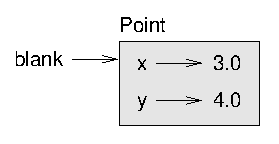
\includegraphics[scale=0.8]{figs/point.eps}}
\caption{オブジェクト図}
\label{fig.point}
\end{figure}
%
変数{\tt blank}は{\tt Point}オブジェクトを参照し、二つの属性を持っていることを示す。各属性は浮動小数点数を参照している。\par
属性の値は普通のように扱える：
\begin{verbatim}
>>> blank.y
4.0
>>> x = blank.x
>>> x
3.0
\end{verbatim}
表式{\tt blank.x}の意味は「{\tt blank}が参照しているオブジェクトに行き、{\tt x}の値を得よ」である。
更にこの場合はその値を変数{\tt x}に代入している。変数{\tt x}と属性{\tt x}の間には何も対立はない。\par
ドット表記は任意の表式のなかで使える。例を示す：
\begin{verbatim}
>>> '(%g, %g)' % (blank.x, blank.y)
'(3.0, 4.0)'
>>> distance = math.sqrt(blank.x**2 + blank.y**2)
>>> distance
5.0
\end{verbatim} \par
インスタンスを関数の引数とすることもできる：
\begin{verbatim}
def print_point(p):
    print('(%g, %g)' % (p.x, p.y))
\end{verbatim}
関数{\tt print\_point}は引数として{\tt point}オブジェクトを受け取り、それを数学的な表記で表示する。
これを発動させるときは引数にインスタンス{\tt blank}を渡せばよい：
\begin{verbatim}
>>> print_point(blank)
(3, 4)
\end{verbatim} \par
この関数の中では{\tt p}は{\tt blank}の別名であるので、関数の中で{\tt p}を変更すると{\tt blank}も変わる。\par
練習問題として、二つの{\tt point}オブジェクトを引数に取り、
二点間の距離を戻り値とする関数{\tt distance\_between\_points}を作成せよ。
%
\section{長方形}
オブジェクトの属性が明白であるものもあるし、そうでなく上手く決めなければならない場合もある。
例として、長方形を表現するクラスを設計することを考えよう。
その位置と大きさを指定するためにどのような属性が必要だろうか？簡単にするために長方形は垂直や水平に置かれたものとする。\par
指定の仕方に少なくとも二つの方法があるだろう：
\begin{itemize}
\item 長方形の一頂点（または中心）の座標、幅、高さを指定する。
\item 対角線上にある二つの頂点の座標を指定する。
\end{itemize}
どちらがよいか決めかねるので、第一の方法を使う。\par
クラス定義は以下のようだ：
\begin{verbatim}
class Rectangle(object):
    """Represents a rectangle

    attributes: width, height, corner
    """
\end{verbatim} 
ドキュメント文字列にある属性{\tt width}, {\tt height}は数、{\tt corner}は{\tt Point}オブジェクトである。 \par
一つの長方形を表現することは{\tt Rectangle}オブジェクトをオブジェクト具現化し、その属性に値を代入することである：
\begin{verbatim}
box = Rectangle()
box.width = 100.0
box.height = 200.0
box.corner = Point()
box.corner.x = 0.0
box.corner.y = 0.0
\end{verbatim} 
表式{\tt box.corner.x}の意味は「{\tt box}が参照するオブジェクトへ行き、{\tt corner}と名付けられた属性を選択し、
そのオブジェクトへ行き、{\tt x}と名付けられた属性を選択せよ」である。
図\ref{fig.rectangle}はこのオブジェクトの{\bf オブジェクト状態図（object diagram）}を示している。
%
 \begin{figure}[htbp]
\centerline
{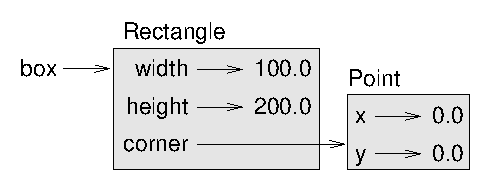
\includegraphics[scale=0.8]{figs/rectangle.eps}}
\caption{オブジェクト図}
\label{fig.rectangle}
\end{figure}
%
他のオブジェクトの属性になっているオブジェクトは{\bf 埋め込まれたオブジェクト（embedded object）}である。
%
\section{戻り値としてのインスタンス}
関数の戻り値にインスタンスがくることがある。
例を示す。関数{\tt find\_center}は引数に{\tt Rectangle}オブジェクトを取り、戻り値にこの{\tt Rectangle}の中心の座標を含む{\tt Point}オブジェクトを返す：
\begin{verbatim}
def find_center(rect):
    p = Point()
    p.x = rect.corner.x + rect.width/2.0
    p.y = rect.corner.y + rect.height/2.0
    return p
\end{verbatim} 
例としてインスタンス{\tt box}を引数にしてみると、その中心の座標が戻ってくる：
\begin{verbatim}
>>>center = find_center(box)
>>>print_point(center)
(50, 100)
\end{verbatim}
%
\section{オブジェクトは変更可能}
オブジェクトの属性の一つに値を代入することでオブジェクトの状態を変えることができる。例えば、一つの長方形の座標は変えずに、widthとheightを変えたいとしたら以下のようにする：
\begin{verbatim}
box.width = box.width + 50
box.height = box.height + 100
\end{verbatim}
オブジェクトを変更する関数を書くこともできる。
例えば、{\tt Rectangle}オブジェクトと二つの数、{\tt dwidth}、{\tt dheight}を引数に持つ
関数{\tt grow\_rectangle}はこの二つの数値分だけ長方形を大きくする関数である：
\begin{verbatim}
def grow_rectangle(rect, dwidth, dheight):
    rect.width += dwidth
    rect.height += dheight
\end{verbatim}
以下はこの関数の効果を示す例である：
\begin{verbatim}
>>> box.width, box.height
(150.0, 300.0)
>>> grow_rectangle(box, 50, 100)
>>> box.width, box.height
(200.0, 400.0)
\end{verbatim}
関数の中では{\tt rect}は{\tt box}の別名である。従って関数内で{\tt rect}を変更すれば、{\tt box}も変更される。\par
練習問題として、引数としてオブジェクト{\tt Rectangle}と二つ数{\tt dx}、{\tt dy}を取り、長方形の
場所の座標{\tt x}と{\tt y}をそれぞれ{\tt dx}と{\tt dy}だけ移動する関数{\tt move\_rectangle}を作成せよ。
%
\section{コピー}
別名呼称は一ヶ所を変えると他に思わぬ効果が出るためプログラムを読み難くしてしまう。
その結果あるオブジェクトを参照する全ての変数の軌跡を追跡することを難しくしてしまう。\par
別名呼称に替わるものとしてコピーがある。モジュール{\tt copy}は任意オブジェクトのコピーを生成する関数{\tt copy}を提供している：
\begin{verbatim}
>>> p1 = Point()
>>> p1.x = 3.0
>>> p1.y = 4.0

>>> import copy
>>> p2 = copy.copy(p1)
\end{verbatim}
{\tt p1}と{\tt p2}は同じデータを含んでいるが、同一の{\tt Point}オブジェクトではない。
\begin{verbatim}
>>> print_point(p1)
(3, 4)
>>> print_point(p2)
(3, 4)
>>> p1 is p2
False
>>> p1 == p2
False
\end{verbatim}
{\tt is}演算子は二つが同一のオブジェクトでないことを意味し、これは予想したことだ。
しかし、{\tt ==}演算子では結果は{\tt True}と出ることを期待したかもしれないが、その予想は外れた。
インスタンスについては既定値として、{\tt ==}演算子は{\tt is}演算子と同じ振る舞いをする。尤も、この振る舞いは変えられるが、これは後の話だ。\par
{\tt copy}関数を使うと{\tt Rectangle}の複製を作ることができるが、埋め込まれたオブジェクト{\tt Point}は違う。
\begin{verbatim}
>>> box2 = copy.copy(box)
>>> box2 is box
False
>>> box2.corner is box.corner
True
\end{verbatim}
図\ref{fig.rectangle2}はオブジェクトの状態図がどうなるかを示した。
この操作はオブジェクトとそれらが参照しているもののコピーは作成するが埋め込まれたオブジェクトは
そのままであるので{\bf 浅いコピー（shallow copy）}と呼ばれる。
 %
\begin{figure}[htbp]
\centerline
{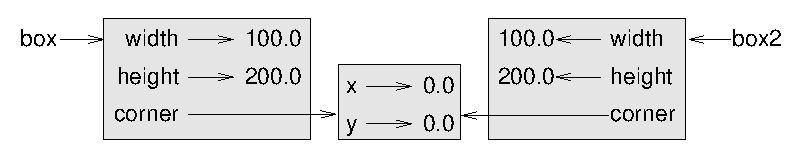
\includegraphics[scale=0.8]{figs/rectangle2.eps}}
\caption{オブジェクト図}
\label{fig.rectangle2}
\end{figure}
%
大部分のアプリケーションではこの事情はあって欲しくないものである。
いまの例でいうとオブジェクト{\tt Rectangle}に対して{\tt grow\_rectangle}を発動させるとコピーされた別のインスタンスは影響を受けない。
しかし、関数{\tt move\_rectangle}の発動では別のインスタンスも影響をうける。こんな振る舞いは混乱するし、エラーの元だ。\par
幸にして、オブジェクトばかりでなく、そのオブジェクトが参照するオブジェクト、
また更にそれらが参照するオブジェクト等々のコピーをも生成する関数{\tt deepcopy}が提供されている。
これを{\bf 深いコピー（deep copy）}と呼ぶ理由は自明だろう。
\begin{verbatim}
>>> box3 = copy.deepcopy(box)
>>> box3 is box
False
>>> box3.corner is box.corner
False
\end{verbatim}
これで{\tt box}と{\tt box3}は完全の別なオブジェクトである。\par
練習問題として、引数として{\tt Rectangle}オブジェクトを受け取り、
新しい{\tt Rctangle}を返す関数{\tt move\_rectangle}の改訂版を作成せよ。
%
\section{デバッギング}
オブジェクトの処理を含むプログラムを扱い始めると新た種類のエラーに遭遇する。
もし存在しない属性にアクセスしようとすると、{\tt AttributeError}が出る：
\begin{verbatim}
>>> p = Point()
>>> p.x = 3
>>> p.y = 4
>>> p.z
AttributeError: Point instance has no attribute 'z'
\end{verbatim}
もし一つのオブジェクトがどうようなものか不明な時は、以下のようなコマンドを使うとよい：
\begin{verbatim}
>>> type(p)
<class '__main__.Point'>
\end{verbatim}
もしある属性をそのオブジェクトが持っているか不明なときは組み込み関数{\tt hasattr}が使える：
\begin{verbatim}
>>> hasattr(p, 'x')
True
>>> hasattr(p, 'z')
False
\end{verbatim}
第一番目の引数は任意のオブジェクトで、第二番目の引数はその属性とした名前の{\bf 文字列}である。\par
オブジェクトがその属性を持っているか不明なときは{\tt try}文を使うこともできる：
\begin{verbatim}
try:
    x = p.x
except AttributeError:
    x = 0
\end{verbatim}
この手法は異なったタイプでも動作する関数を書こうとする上で便利なものである。このテーマの詳細は
第17.9節で扱う。
%
\section{語句}
\begin{description}

\item[クラス（class）：] ユーザ定義型。クラスの定義によって新しいクラスオブジェクトが生成される。
%\index{class}

\item[クラスオブジェクト（class object）：] ユーザ定義型に関する情報を含むオブジェクト。クラスオブジェクトは
その型のインスタンスを生成するときに使われる。
%\index{class object}
%\index{object!class}

\item[インスタンス(instance)：] 一つのクラスを具現化したオブジェクト。
%\index{instance}

\item[具現化（instantiate）：] 新規のオブジェクトを作ること。
%\index{instantiate}

\item[属性（attributes）：] 一つのオブジェクトに付随した名前の付いた値。
%\index{attribute!instance}
%\index{instance attribute}

\item[埋め込まれたオブジェクト（embedded　object）：] 他のオブジェクトの属性として使われたオブジェクト。
%\index{embedded object}
%\index{object!embedded}

\item[浅いコピー（shallow copy）：] 埋め込まれたオブジェクトへの参照を残したままオブジェクトの複製を作る。
\index{shallow copy}

\item[深いコピー（deep copy）：] そのなかに埋め込まれたオブジェクトがあるときその複製をも作るかたちでオブジェクトの複製を作る。
%\index{deep copy}

\item[オブジェクト状態図（object diagram）：] オブジェクト、その属性、その属性が参照している値を明示するグラフ表現。
%\index{object diagram}
%\index{diagram!object}

\end{description}
%
\section{練習問題}
\noindent
{\bf 練習問題\tp.1} {\tt Circle}という名前のクラスを定義せよ。
その属性は{\tt center}と{\tt radius}で{\tt center}は{\tt Point}オブジェクトであり、
{\tt radius}は数値である。\par
次にこの{\tt Circle}オブジェクトを{\tt center}の値を{\tt 150,100)}
そして{\tt radius}の値を{\tt 75}の初期値で具現化せよ。\par
以下幾つかの関数を作成せよ：
\begin{itemize}
\item 一つの{\tt Circle}オブジェクトと一つの{\tt Point}オブジェクトを引数とする関数{\tt point\_in\_circle}
を作成せよ。この関数のはこの{\tt Point}がこの{\tt Circle}の内側もしくは
境界上にあるならば{\tt Ture}を戻り値として返す。
\item 一つの{\tt Circle}オブジェクトと一つの{\tt Rectangle}オブジェクトを引数と
する関数{\tt rect\_in\_circle}を作成せよ。
この関数はこの{\tt Rectangle}全体がこの{\tt Circle}の内側もしくは
境界上にあるならば{\tt Ture}を戻り値として返す。
\item 一つの{\tt Circle}オブジェクトと一つの{\tt Rectangle}オブジェクトを引数と
する関数{\tt rect\_circle\_overlap}を作成せよ。
この関数はこの{\tt Rectangle}の頂点の一つでもこの{\tt Circle}の内側に
あるならば{\tt Ture}を戻り値として返す。\par
もう少し挑戦的な課題として、この{\tt Rectangle}の辺のどこか
の部分がこの{\tt Circle}の内側に
あるならば{\tt Ture}を戻り値として返すとした関数を作成せよ。
\end{itemize}
解答例：\url{https://thinkpython.com/code/Circle.py}.\\

\noindent
{\bf 練習問題\tp.2} {\tt Turtle}オブジェクトと{\tt Rectangle}オブジェクト
とを引数に持ち、この{\tt Turtle}でこの{\tt Rectangle}を描画する関数
{\tt draw\_rect}を作成せよ。{\tt Turtle}オブジェクトの使い方は第４章を参照のこと。\\
また同様に円を描画する関数{\tt draw\_circle}を作成せよ。\\
解答例：\url{https://thinkpython.com/code/draw.py}
%
\chapter{クラスと関数}
新しい型の作り方がわかったので、次のステップはこのようなユーザ定義型のオブジェクト
を仮引数に持ち、戻り値もこれらの型のオブジェクトを取るような関数を作ることである。
またこの章では「関数プログラミング手法」と二つの新たなプログラム開発計画法についても触れる。\par
この章のサンプルコードは\url{https://thinkpython.com/code/Time1.py}にある。また
練習問題の解答例は\url{https://thinkpython.com/code/Time1_soln.py}.にある。
%
\section{時刻}
ユーザ定義型のもう一つの例として一日の内の時刻を記録する{\tt Time}を取り上げる。
そのクラス定義は以下のようだ：
\begin{verbatim}
class Time:
    """Represents the time of day.

    attributes: hour, munute, second
    """
\end{verbatim}
{\tt Time}オブジェクトを生成し、属性に値を代入してみる：
\begin{verbatim}
time = Time()
time.hour = 11
time.minute = 59
time.second = 30
\end{verbatim}
%
\begin{figure}[htbp]
\centerline
{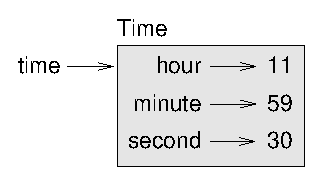
\includegraphics[scale=0.8]{figs/time.eps}}
\caption{オブジェクト図}
\label{fig.time}
\end{figure} 
%
図\ref{fig.time}にこのオブジェクトの状態図を示した。\par
練習問題として、引数として{\tt Time}オブジェクトを取り、
{\tt hour:minute:second}の形式で時刻表示をする関数{\tt print\_time}を作成せよ。
ヒント：記述子{\verb"'%.2d'"}を使うと整数を先頭に{\tt 0}を詰めて二桁で表現する。
%
\section{純関数}
以下では時刻の和を求める関数{\tt add\_time}を作成することにする。
ここでは二つの関数が開発の途上で検討されることになる。
それらは純関数と修正関数である。
またこの二種類の関数は単純なものから初めて徐々に複雑なものにして行く開発計画で
{\bf 原型とパッチ（prototype and patch）}と呼ばれるものに対応している。\par
関数{\tt add\_time}の原型は以下のようなものだろう：
\begin{verbatim}
def add_time(t1, t2):
    sum = Time()
    sum.hour = t1.hour + t2.hour
    sum.minute = t1.minute + t2.minute
    sum.second = t1.second + t2.second
    return sum
\end{verbatim}
この関数では新たに{\tt sum}という{\tt Time}オブジェクトを生成、属性を初期化、そのオブジェクトを戻り値としている。
これは引数として受け取ったオブジェクトを何も変えないで、しかも値を表示するとか、
ユーザ入力を求めるとかの効果もないという意味で{\bf 純関数（pure function）}と呼ぶ。 \par
この純関数をテストするために
映画``Monty Python and the Holly Grail"の開始時間{\tt start}という{\tt Time}オブジェクトとこの映画の
上演時間（１時間３５分）を保存する{\tt duration}という{\tt Time}オブジェクトを生成する。\par
{\tt add\_time}で何時にこの映画が終わるか分かる：
\begin{verbatim}
>>> start = Time()
>>> start.hour = 9
>>> start.minute = 45
>>> start.second = 0

>>> duration = Time()
>>> duration.hour = 1
>>> duration.minute = 35
>>> duration.second = 0
>>> done = add_time(start, duration)
>>> print_time(done)
10:80:00
\end{verbatim}
結果の{\tt 10:80:00}はわれわれが欲しいものではない。
問題は秒や分で足し合わせた結果60より大きくなったときの処理をしていないからである。
この状況が起きたときは、余分な秒を分に「桁上げ」、余分な分を時に「桁上げ」しなければならない。\par
これを考慮した改訂版である：
\begin{verbatim}
def add_time(t1, t2):
    sum = Time()
    sum.hour = t1.hour + t2.hour
    sum.minute = t1.minute + t2.minute
    sum.second = t1.second + t2.second

    if sum.second >= 60:
        sum.second -= 60
        sum.minute +=1

    if sum.minute >= 60:
        sum.minute -= 60
        sum.hour += 1
        
    return sum
\end{verbatim}
改訂版は正しいが、コードは大きめになり初めている。次章ではこれに替わる修正の方法を示す。
%
\section{修正関数}
ある場合には引数として受け取ったオブジェクトを修正する関数の使用が有益なことがある。
この場合にはこの関数を呼んだ側にも修正が反映される。この機能を取り入れた関数を{\bf 修正関数（modifiers）}と呼ぶ。\par
与えられた秒数だけ{\tt Time}オブジェクトの時刻を増加させる関数{\tt increment}は素直に修正関数として書くことができる：
\begin{verbatim}
def increment(time, seconds):
    time.second += seconds

    if time.second >= 60:
        time.second -= 60
        time.minute +=1

    if time.minute >= 60:
        time.minute -= 60
        time.hour += 1
\end{verbatim}
第一行目が基本演算で、残りは前にみたような特別な場合の処理である。\par
ところでこの関数は正しいだろうか？
第二の引数{\tt second}が60秒よりずうっと大きな値であるとどうなるだろうか？その場合には桁上がりは一度では足りない。
つまり、{\tt Time}オブジェクトの{\tt second}属性の値が60より小さくなるまで桁上がりを続ける必要がある。
一つの解決策は{\tt if}文を{\tt while}文に置き換えることだが、効率が悪い。
練習問題として、関数{\tt increment}を正せ。繰り返しのループ無しでこれを達成せよ。\par
修正関数でできることは何でも純関数でできる。実際、純関数のみが許されているプログラミング言語もある。
純関数を使ったプログラムが修正関数を使ったものと比べ開発や速くエラー誘発が少ないとする証拠がある。
しかし修正関数が便利なこともあり、関数プログラムがそんなに効率が出ないときもある。\par
一般に特に問題がなければ純関数を使い、それを使う特別な理由があるときのみ修正関数を使うことを勧める。
このアプローチはいわば{\bf 関数プログラミング作法（functional programming style）}と言ってもよい。 \\
練習問題として、関数{\tt increment}の純関数版を作成せよ。
引数の{\tt Time}オブジェクトを修正する替わりに、結果を新たに生成した{\tt Time}オブジェクトとして戻せ。
%
\section{原型と開発計画}
ここまで示してきたプログラム開発法は「原型とそのパッチ」と呼ばれる方法である。
各関数について、まず基本的な計算をする原型を作成し、その後にこれをテストし、必要な修正を施す。\par
この手法は問題の深い理解がまだできていないとき特に有効な方法となる。
しかし、この手法は徐々に複雑化するためどれほど複雑にしたらよいのかが不明なので必要以上にコードが複雑になる傾向がある。\par
別の手法は{\bf 計画に基づいた開発手法（planned development）}である。
これは高いレベルの問題考察でプログラミングをより容易にしてくれる手法である。
{\tt Time}オブジェクトに関して言えば、その洞察は60進法（\url{http://en.wikipedia.org/wiki/Sexagesimal}
を参照せよ。）を基礎にした三つの数字の問題で、
属性{\tt second}はその60進数の一桁目の数字であり、属性{\tt minute}は二桁目、
属性{\tt hour}は三桁目の数字であることを教えてくれる。
関数{\tt add\_time}や{\tt increment}では桁上がりを行うことで実質的に60進法の和を実行していたことになる。\par
このような考察は全問題に対して異なる手法が採れることを教えてくれる。
つまり、{\tt Time}オブジェクトをコンピュータが桁上がりを自動的に処理できる10進数（つまり整数）に変換してしまうことだ。\par
{\tt Time}オブジェクトを整数に変換は以下のようである：
\begin{verbatim}
def time_to_int(time):
    minutes = time.hour * 60 + time.minute
    seconds = minutes * 60 + time.second
    return seconds
\end{verbatim}
この逆に、整数を{\tt Time}オブジェクトに変換するコード
（関数{\tt divmod}二つの引数を取り、最初の引数を第二で割った商と余りをタプルとして戻す）は以下のようになる：
\begin{verbatim}
def int_to_time(seconds):
    time = Time()
    minutes, time.second = divmod(seconds, 60)
    time.hour, time.minute = divmod(minutes, 60)
    return time
\end{verbatim} \par
これらの関数は期待通り動くことを確認するためにいろいろなテストをやってみるかもしれないが、
一つの面白い実験は{\verb"time_to_int(int_to_time(x)) == x"}が成り立つことを確かめることだ。これは一貫性のテストの例にもなっている。\par
関数が期待通りに動くことが確かめられたら、関数{\tt add\_time}の作成に使ってきる：
\begin{verbatim}
def add_time(t1, t2):
    seconds = time_to_int(t1) + time_to_int(t2)
    return int_to_time(seconds)
\end{verbatim}
この版はすっきりしているし、確認が楽である。練習問題として、{\tt time\_to\_int}や{\tt int\_to\_time}
を使って関数{\tt increment}も同様に書き換えよ。\par
ある面では60進法数と10進法数への変換、またはその逆変換は時間についての観念のよる操作より難しいかもしれない。
この変換はより抽象的で、日常の時間に対するわれわれの直感のほうが良いかもしれない。
しかし、一度60進法数としての時間につての洞察ができ、その変換プログラムを作ってしまうと、
より短く、読むことやデバッグがより易しく、より信頼性の高いプログラムを作ることができる。\par
また、この方法を取ると機能の追加をするのが楽である。
例えば、二つの時間の差を求める問題を考えてみよう。従来の方法では、
上位の桁からの借りが必要になる。変換関数を使う方法ではもっと簡単で、従って正常に動くプログラムが作れる。
%
\section{デバッギング}
{\tt Time}オブジェクトは{\tt minute}や{\tt second}が0と60の間（0は含み60は含まない）の値を持っていて、
{\tt hour}が正の値であると健全である。またhourや{\tt minute}の値は整数値であるべきだが、{\tt second}は小数点数であってもよい。
このような要求はそれが何時も満たされていることが求められるものなので、
{\bf 不変性（invariants）}と呼ばれている。換言すれば、それが満たされていないと何かが間違っているということになる。\par
この不変性をチェックするようにプログラムを書くと、エラーの検出やその原因解明にとっての助けになる。
例えば、{\tt Time}オブジェクトを引数としてそれば不変性の一つでも破っているときは{\tt False}を返す関数{\tt valid\_time}が作れる：
\begin{verbatim}
def valid_time(time):
    if time.hour < 0 or time.minute < 0 or time.second < 0:
        return False
    if time.minute >= 60 or time.second >= 60:
        return Flase
    return True
\end{verbatim}
関数の先頭でこのチェックをして引数の妥当性を調べることができる：
\begin{verbatim}
def add_time(t1, t2):
　　if not valid_time(t1) or not valid_time(t2):
        raise ValueError, 'invalid Time object in add_time'
    seconds = time_to_int(t1) + time_to_int(t2)
    return int_to_time(seconds)
\end{verbatim}
または{\tt assert}文を使い、条件が満たされていないと例外を発生させることもできる：
\begin{verbatim}
def add_time(t1, t2):
　　assert valid_time(t1) and valid_time(t2)
    seconds = time_to_int(t1) + time_to_int(t2)
    return int_to_time(seconds)
\end{verbatim}
{\bf {\tt assert}文（assert statement）}は通常に実行されるコードとエラー検出用のコードを区別するので役に立つ。
%
\section{語句}
\begin{description}

\item[原型とパッチ（prototype and patch）：] 大雑把なプログラムを書き、それをテストして見つかったエラーを修正するといった開発計画。
%\index{prototype and patch}

\item[計画に基づいた開発手法（planned development）：] 徐々に精査する開発法や原型とパッチ方式より問題自体を精査して高いレベルで
問題を捉えなおしより計画性をもった開発計画。
%\index{planned development}

\item[純関数（pure function）：] 引数として受け取ったオブジェクトに如何なる変更も施さない関数。多くは戻り値を持つ。
%\index{pure function}

\item[修正関数（modifiers）：] 引数として受け取った一つまたはそれ以上のオブジェクトに修正を施すような関数。
%\index{modifier}

\item[関数プログラミング作法（functional programming style）：] 多くの関数が純関数として計画されたプログラミング手法。
%\index{functional programming style}

\item[不変性（invariants）：] プログラムの実行過程で常に「真」の状態にあるべきとされる条件。
%\index{invariant}

\item[{\tt assert}文（assert statement）：] 条件を調べ満たされていないときには例外（AssertionError）を
発生させる。 

\end{description}
%
\section{練習問題}
この章で使ったコードは以下から利用できる：\url{https://thinkpython.com/code/Time1.py}。
また、練習問題の解答例は以下からダウンロードできる：\\
\url{https://thinkpython.com/code/Time1_soln.py}。\\

\noindent
{\bf 練習問題\tp.1} {\tt Time}オブジェクトと数を引数として、この{\tt Time}オブジェクトにこの数を乗じた{\tt Time}オブジェクトを返す関数{\tt mul\_time}を作成せよ。
更にこの関数{\tt mul\_time}を使って、レースの所要時間を表す{\tt Time}オブジェクトと距離（マイル）を表す数を引数として、
レースの平均ペース（時間毎マイル）を示す{\tt Time}オブジェクトを返す関数を作成せよ。\\

\noindent
{\bf 練習問題\tp.2} モジュール{\tt datetime}はこの章で議論したと同じような{\tt date}や{\tt time}オブジェクトを提供しているが、
さらに多くのメソッドや操作を含んでいる。詳しくは\url{http://docs.python.org/3/library/datetime.html}.を参照せよ。
\begin{enumerate}
\item 日日を引数にとり、曜日を返す関数{\tt datetime}を作成せよ。
\item 誕生日の日付を受け取り、ユーザの年齢と次ぎの誕生日までの日数、時、分、秒を表示するプログラムを作成せよ。
\item 異なった日に生まれた二人にとって、一人が他の日数の二倍になる日が存在する。
これは二人にとって「二倍日」である。二つの誕生日を引数として受け取り、この二人の「二倍日」を計算するプログラムを作成せよ。
\item もう少し挑戦的な問題として、一般に二人の誕生日を引数として、一人の年齢が他の年齢{\tt n}倍のなる日を計算するプログラムを作成せよ。
\end{enumerate}
解答例：\url{https://thinkpython.com/code/double.py}
%
\chapter{クラスとメソッド}
これまでPythonの オブジェクト指向の特徴の幾つかを使ってきたが、前二章のプログラムはユーザ定義型
とそれに作用する関数類の関係を表現したものでないという意味で真のオブジェクト指向プログラムではない。
次のステップは前二章で展開した関数を定義型との関係を陽に表現するメソッドに変換することである。
この章のサンプルコードは\url{https://thinkpython.com/code/Time2.py}にある。また練習問題の解答例
は\url{https://thinkpython.com/code/Point2_soln.py}.にある。
%
\section{オブジェクト指向の特徴}
Pythonはオブジェクト指向プログラミングを行う機能を提供しているという意味で
{\bf オブジェクト指向言語（object-oriented programming language）}である。
オブジェクト指向プログラミングは以下のような特徴を持っている：
\begin{itemize}
\item プログラムはオブジェクトの定義、メソッドの定義を含む。
\item 多くの操作がオブジェクトに対する演算として表現される。
\item 各オブジェクトは現実世界の実体や概念に対応していて、
オブジェクトに対し適用される関数は現実世界の実体が相互作用している様に対応している。
\end{itemize}
例えば、第16章で定義した{\tt Time}クラスは人々が時間を記録する様に対応し、その関数は人々がその時間について行う操作に対応している。
同様に第15章で現れた{\tt Point}クラスや{\tt Rectangle}クラスは数学的な概念に対応して定義される。 \par
いままではPythonが提供しているオブジェクト指向の特徴を利用してこなかった。それらの特徴は厳格には必要でない。
それらの特徴の多くはこれまで作ってきたプログラムの異なった表現による解を提供するにすぎない。
しかし、多くの場合、この別表現はより簡便で、より正確にプログラムの構造を伝達することができる。 \par
例えば、{\tt Time}クラスでは、クラスの定義とそれに続く関数定義との間には関連があるかどうかは自明ではない。
詳しくみると、全ての関数の引数の内少なくとも一つは{\tt Time}オブジェクトであることが分かる。\par
この観察はある特別なクラスに付随する関数、つまり{\bf メソッド（method）}の導入の契機になる。
これまで文字列、リスト、辞書そしてタプルのためのメソッドをみてきた。この章ではユーザ定義型に対するメソッドを定義する。\par
メソッドは意味論的には関数と同じであるが、構文的には二つの点で関数とは異なる：
\begin{itemize}
\item メソッドはクラスとの関連を明白にするため、クラスの内部で定義される。
\item メソッド起動に対する構文は関数を呼ぶ場合の構文とは異なる。
\end{itemize}
次の数節では前二章に登場した関数を取り上げ、それらをメソッドに変換する。変換自体は極めて機械的である。
ステップに従えばできる。この変換に問題を感じないのであれば、何をするときも、二つ表現の内から最良と思うものを選択して使ってもらえばよい。
%
\section{オブジェクトの{\tt print}}
第16章では{\tt Time}クラスを定義し、練習問題16.1では{\tt print\_time}という関数を作成した：
\begin{verbatim}
class Time(object):
    """Represents the time of day."""

def print_time(time):
    print('%02d:%02d:%02d' % (time.hour, time.minute, time.second))
\end{verbatim}
この{\tt print\_time}関数を呼ぶためには引数に{\tt Time}オブジェクトを渡さなければならない：
\begin{verbatim}
>>> start = Time()
>>> start.hour = 9
>>> start.minute = 45
>>> start.second = 0
>>> print_time(start)
09:45:00
\end{verbatim} 
{\tt print\_time}をメソッドにするために、
しなければならないことの全てはこの関数定義をクラス定義の中に移動することだ（インデントの調整も忘れずに）：
\begin{verbatim}
class Time(object):
    def print_time(time):
        print('%02d:%02d:%02d' % \
          (time.hour, time.minute, time.second))
\end{verbatim} \par
さて、この{\tt print\_time}を呼ぶ方法には二通りある。最初は（あまり普通はやらないが）関数呼び出しの構文である：
\begin{verbatim}
>>> Time.print_time(start)
09:45:00
\end{verbatim}
このドット表記では、{\tt Time}はクラス名、{\tt print\_time}はメソッド名、{\tt start}は引数である。\par
第二は（普通にやる）メソッド構文によりものだ：
\begin{verbatim}
>>> start.print_time()
09:45:00
\end{verbatim}
このドット表記では、{\tt print\_time}はメソッド、{\tt start}はこのメソッドを発動させるオブジェクトで、
{\bf 主語（subject）}と言う。文章の主語がその文章が何についてであるか示すと正に同じように、
メソッドを発動する主語はそのメソッドが何についてあるかを示すものである。\par
メソッドの中では主語は第一番目の仮引数として代入される。今の場合は{\tt start}が仮引数{\tt time}に代入される。
慣例で、メソッドの第一仮引数は{\tt self}という名前が使われる。したがって、より通常の形に{\tt print\_time}を書けば以下のようになる：
\begin{verbatim}
    def print_time(self):
        print('%02d:%02d:%02d' % \
          (self.hour, self.minute, self.second))
\end{verbatim}
この慣例で書く理由は直接的な比喩にある：
\begin{itemize}
\item 関数呼び出し{\tt print\_time(start)}の構文は関数が活動主体であると示唆している。
差詰め、「さあ、{\tt print\_time}よ。ここにお前さんがプリントするオブジェクトが一つあるよ」と言っているようなものだ。
\item オブジェクト指向プログラミングでは、オブジェクトが活動主体である。
{\tt start.print\_time()}のようにメソッドを起動することは、「やあ、{\tt start}。自分のことは自分で処理してください」
と言っているようなものだ。
\end{itemize}
このような見方の変更はより洗練されたものかもしれないが、それが有用であることは自明ではない。
これまでの例では有用とはなっていない。
しかし、責任主体を関数からオブジェクトに移すことは時として用途が多い関数を書き、
よりメンテナンスが容易で再利用可能な関数を書くことを可能にするのだ。\\
練習問題として、関数{\tt time\_to\_int}（16.4節）をメソッドとして書き換えよ。
関数{\tt int\_to\_time}はメソッドに書き換える理由がない。これを発動させるオブジェクトがあるかな？
%
\section{別な例}
16.3節で登場した関数{\tt increment}をメソッドとして書き換える：
\begin{verbatim}
# クラスTimeの定義に中で
    def increment(self, seconds):
        seconds += self.time_to_int()
        return int_to_time(seconds)
\end{verbatim}
ここで{\tt time\_to\_int}は直前の練習問題のようにメソッドとして書かれているものとする。
さらに、このメソッドは純関数をメソッドにしたもので、修正関数ではないことにも注意すること。\par
この{\tt increment}の発動は以下のようになる：
\begin{verbatim}
>>> start.print_time()
09:45:00
>>> end = start.increment(1337)
10:07:17
\end{verbatim}
主語{\tt start}が関数の第一仮引数{\tt self}に代入される。引数{\tt 1337}は第二仮引数{\tt seconds}に代入される。\par
この機構は特にエラーに遭遇したときに混乱の元になる。例えば、{\tt increment}に二個の引数を与えて発動させると以下のようにエラーになる：
\begin{verbatim}
>>> end = start.increment(1337, 460)
TypeError: increment() takes 2 positional arguments but 3 were given
\end{verbatim}
このエラーメッセージには最初混乱する。括弧の中は二つの引数になっているからだ。
しかし、主語それ自体も引数として考えるので、合わせて三個ということになる。\par
序ながら{\bf 位置固定引数（positional argument）}と言っているのは仮引数名で指定する
キーワード引数でない引数である。例えば以下のような関数呼び出しを例にとると：
\begin{verbatim}
sketch(parrot, cage, dead=True)
\end{verbatim}
{\tt parrot}と{\tt cage}は位置固定引数で、{\tt dead}はキーワード引数である。
%
\section{もっと複雑な例}
関数{\tt is\_after}（16.1節）は引数に二つの{\tt Time}オブジェクトを取るから少し複雑になる。
この場合最初の仮引数の名前は{\tt self}、二番目を{\tt other}とするのが慣例である：
\begin{verbatim}
# クラスTimeの定義に中で
    def is_after(self, other):
         return self.time_to_int() > other.time_to_int()
\end{verbatim}
このメソッドを使うには、一つのオブジェクトでこれを発動させ、他のオブジェクトは引数としてこのメソッドに渡す：
\begin{verbatim}
>>> end.is_after(start)
True
\end{verbatim}
この構文の愉快なのは英文を読むような順序に並んでいることだ、つまり、``end is after start?"。
%
\section{{\tt init}メソッド}
{\tt init}メソッド（``initialization"の省略）はオブジェクト具現化の際に発動される特殊なメソッドである。
正式名は{\verb"__init__"} （二つのアンダースコア記号にinitが続き更に二つのアンダースコア記号）。\par
{\tt Time}クラスの{\tt init}メソッドは以下のようなものだろう：
\begin{verbatim}
# クラスTimeの定義に中で
    def __init__(self, hour=0, minute=0, second=0):
        self.hour = hour
        self.minute = minute
        self.second = second
\end{verbatim}
{\verb"__init__"}の引数の名前を属性と合わせることは習慣だ。
文{\tt self.hour = hour}の意味は引数{\tt hour}の値は{\tt self}の属性{\t hour}の値として保存されるということである。
\begin{verbatim}
>>> time = Time()
>>> time.print_time()
00:00:00
\end{verbatim}
もし引数一つを与えると、その値は{\tt hour}の値を再定義する：
\begin{verbatim}
>>> time = Time(9)
>>> time.print_time()
09:00:00
\end{verbatim}
もし引数二つを与えると、それらは{\tt hour},{\tt  minute}の値を再定義する：
\begin{verbatim}
>>> time = Time(9, 45)
09:45:00
\end{verbatim}
引数三つを与えると既定値の全てが無効になる。\par
練習問題として、{\tt Point}クラスの{\tt init}メソッドを作れ。引数は{\tt x}と{\tt y}で、対応する属性に代入されるようにせよ。
%
\section{{\tt \_\_str\_\_}メソッド}
{\verb"__str__"}メソッドはオブジェクトの文字列による表現を返す特殊なメソッドである。\par
{\tt Time}オブジェクトのための{\tt str}メソッドは以下のようなものだ：
\begin{verbatim}
# クラスTimeの定義に中で
    def __str__(self):
        return '%02d:%02d:%02d' % \
          (self.hour, self.minute, self.second)
\end{verbatim}
{\tt Time}オブジェクトを{\tt print}しようとすると、{\tt str}メソッドが発動される：
\begin{verbatim}
>>> time = Time(9, 45)
>>> print(time)
09:45:00
\end{verbatim}
わたしが新しいクラスを書くときは、
殆ど常にメンテナンスの容易さから{\verb"__init__"}メソッドを書き、デバッギングに有用なので{\verb"__str__"}メソッドを書くことにしている。\par
練習問題として、{\tt Point}クラスの{\tt str}メソッドを作成し、{\tt Point}オブジェクトを一つ生成し、それを{\tt print}せよ。
%
\section{演算子の多重定義}
特殊なメソッドの定義によって、ユーザ定義型のオブジェクトに対する演算の振る舞いを変更することができる。
例として、{\tt Time}クラスの{\verb"__add__"}メソッドで加算演算子{\tt +}を定義してみよう：
\begin{verbatim}
# クラスTimeの定義に中で
    def __add__(self, other):
         seconds = self.time_to_int() + other.time_to_int()
         return int_to_time(seconds)
\end{verbatim}
これを使ってみる：
\begin{verbatim}
>>> start = Time(9, 45)
>>> duration = Time(1, 35)
>>> print start + duration
11:20:00
\end{verbatim}
{\tt Time}オブジェクトの{\tt +}演算子を使うとPythonはこの{\verb"__add__"}を発動する。
結果を{\tt print}しようとすると、{\verb"__str__"}が発動される。\par
ユーザ定義型のオブジェクトに対して演算子の振る舞いを変更することを{\bf 演算子の多重定義（operator overloading）}と言う。
Pythonの全ての演算子には{\verb"__add__"}のような対応する特殊メソッドがある。詳細は
\url{http://docs.python.org/3/reference/datamodel.html#specialnames}.を参照せよ。\par
練習問題として、{\tt Point}クラスのオブジェクトに対する{\tt add}メソッドを作成せよ。
%
\section{型別処理}
前の節では二つの{\tt Time}オブジェクトを被演算子とする{\tt add}メソッドを作成したが、
一つの{\tt Time}オブジェクトに整数型の数を加えることも考えられる。
以下は引数{\tt other}の型をチェックする{\verb"__add__"}メソッド改訂版で、関数{\tt add\_time}か、{\tt increment}かの
呼び出しに繋げる：
\begin{verbatim}
# クラスTimeの定義に中で
    def __add__(self, other):
        if isinstance(other, Time):
            return self.add_time(other)
        else:
            return self.increment(other)

    def add_time(self, other):
        seconds = self.time_to_int() + other.time_to_int()
        return init_to_time(seconds)

    def increment(self, seconds):
        seconds += self.time_to_int()
        return int_to_time(seconds)
\end{verbatim}
組み込み関数{\tt isinstance}は値とクラスオブジェクトを引数として受け取り、
その値がそのクラスのインスタンスであると{\tt True}を返す。
もし{\tt other}が{\tt Time}オブジェクトであると、{\verb"__add__"}メソッドは{\tt add\_time}を発動させる。
そうでないときは{\tt increment}を発動させる。
引数の型によって異なった計算処理を行うのでこのような演算を{\bf 型別処理（type-based dispatch）}と呼ぶ。\par
異なった型の演算に使ってみる：
\begin{verbatim}
>>> start = Time(9, 45)
>>> duration = Time(1, 35)
>>> print(start + duration)
11:20:00
print(start + 1337)
10:07:17
\end{verbatim}
不幸にしてこの加算演算は交換可能でない。整数を被演算子の最初に置くとエラーになる。
\begin{verbatim}
>>> print(1337 + start)
TypeError: unsupported operand type(s) for +: 'int' and 'instance'
\end{verbatim} \par
問題は{\tt Time}オブジェクトに整数を加えることを要請する替わりに、
Pythonは整数に{\tt Time}オブジェクトを加算することを要請することになり、どうしてよいか分からなくなっていることである。
しかし、上手い解決策がある。{\verb"__radd__"} (``right side add"の略)は
特殊なメソッドで{\tt Time}オブジェクトが演算子{\tt +}の右側にあるときにこのメソッドが発動される。 \par
今の場合の定義は以下のようになる：
\begin{verbatim}
# クラスTimeの定義に中で
    def __radd__(self, other):
        return self.__add__(other)
使ってみる：
>>> print(1337 + start)
10:07:17
\end{verbatim} 
練習問題として、クラス{\tt Point}で{\tt Point}オブジェクトでもタプルでも有効な{\tt add}メソッドを作成せよ。
\begin{itemize}
\item 第二被演算子も{\tt Point}オブジェクトであるときには、戻り値はその被演算子の{\tt x}座標の和、{\tt y}座標の和を要素とする
新規の{\tt Point}オブジェクトになる。
\item 第二被演算子がタプルのときにはタプルの初めの要素を{\tt x}座標に加え、第二の要素を{\tt y}座標に加えた新たな{\tt Point}オブジェクトを戻す。
\end{itemize}
%
\section{多態性}
型別処理は必要なときは便利にものだが、（幸いにして）常に必要になる訳ではない。
よくあるあこであるが、異なった型の引数に対して正確に動作する関数を書くことによってこれを避けることができる。
例として11.2節で取りあげた{\tt histogram}では一つの単語の中の文字頻度をカウントするのに使った。
\begin{verbatim}
def histogram(s):
    d = dict()
    for c in s:
        if c not in d:
            d[c] = 1
        else:
            d[c] += 1
    return d
\end{verbatim}
この関数はその要素がハッシュ可能ならば、つまりキーとして使えるならば、引数はリスト、タプル、それに辞書でさえ有効だ。以下はリストの例である：
\begin{verbatim}
>>> t = ['spam', 'egg', 'spam', 'spam', 'bacon', 'spam']
>>> histogram(t)
{'bacon': 1, 'egg': 1, 'spam': 4}
\end{verbatim} \par
いくつかの型に対しても有効な関数は{\bf 多態的（polymorphic）}だと言う。
多態性はコードの再利用に役立つ。
例えば、組み込み関数{\tt sum}は配列の要素の総和を求める関数であるが、
加算演算子が定義されている要素であれば、如何なる配列でも構わない。
\begin{verbatim}
>>> t1 = Time(7, 43)
>>> t2 = Time(7, 41)
>>> t3 = Time(7, 37)
>>> total = sum((t1, t2, t3))
>>> print(total)
23:01:00
\end{verbatim} 
一般に関数内の全ての操作がある型に対して有効であるならば、その関数はその型に対して有効である。\par
多態性の面白さは既に作成した関数が当初計画しないでいた型に対しても有効だというのを発見すると言った予期しないことがあることだ。
%
\section{デバッギング}
クラスの属性はプログラムの実行中に任意に追加することができるが、もし型に対して厳格な考え方を持つなら、
同じ型のオブジェクトが異なった属性を持つことは疑惑に満ちた習慣だ。オブジェクトの初期化の際に必要な属性を初期化しておくことは健全であろう。
あるオブジェクトがある特定の属性を持っているかどうかを調べるには組み込み関数{\tt hasattr}が役に立つ（15.7節を参照のこと）。\par
あるオブジェクトの属性にアクセスするもう一つの方法は組み込み関数{\tt vars}を使うことだ。
これはこのオブジェクトを引数に取り、そのオブジェクトの属性名（文字列である）とその値を辞書として戻す。
\begin{verbatim}
>>> p = Point(3, 4)
>>> vars(p)
{'y': 4, 'x': 3}
\end{verbatim}
この機能をデバッギングに使うために、簡便な関数を作成する：
\begin{verbatim}
def print_attributes(obj):
    for attr in vars(obj):
        print(attr, getattr(obj, attr))
\end{verbatim}
{\tt print\_attributes}はオブジェクトの辞書を横断的に眺め、その属性と対応する値を表示する。
組み込み関数{\tt getattr}はオブジェクトと属性を引数に取り、属性の値を返す関数である。
%
\section{インタフェースと実装}
オブジェクト指向によるプログラム設計の一つの目標はソフトウエアをより管理・維持し易くすることである。
この意味するところはシステムの他の部分の変更があってもプログラムが動くようにしておくことができ、
且つ、その変更に適合するようにプログラムを変更できることだ。 \par
この目標を達成するための設計原理はインタフェースと実装を分離して置くことである。
オブジェクトに関して言えば、クラスが提供するメソッドはその属性が如何に表現されるかに依らないようにすべきである。\par
例えば、この章では時刻を表現するクラスを作成した。
このクラスが提供するメソッドは{\tt time\_to\_int}、 {\tt is\_after}、そして{\tt add\_time}である。これらのメソッドはいくつかの方法で実装できる。
実装の細部は時刻の表現の仕方に依存している。この章では、{\tt Time}オブジェクトの{\tt hour}, {\tt minute}, {\tt second}という属性がそれである。
他の表現方法として、深夜12時からの経過時間を秒にした一つ整数で表現することもできる。
この実装に沿っていくつかのメソッドが作られることになる。{\tt is\_after}などは容易に書けるメソッドだ。書くのが難しいメソッドもあるだろう。\par
新たなクラスの展開に伴って、もっと改良された実装を見つけるかもしれない。
プログラムの他の場所でこのクラスを使っていたとすると、この実装変更に伴ってインタフェースの変更が伴うとするとこれは時間の浪費とエラーの元になる。
しかし、インタフェースを注意深く設計して置くとインタフェースの変更無しに実装の変更ができる。つまり、プログラムの他の部分への変更はナシで済む。\par
インタフェースを実装から分離しておくということは属性を隠せということだ。
プログラムの他の部分（クラス定義の外）では、メソッドを使いオブジェクトの状態を読み、変更を行うようにするのだ。
属性に直接にアクセスしないようにするわけだ。
このような原理を{\bf 情報隠蔽（information hiding）}と言う。
%
\section{語句}
\begin{description}

\item[オブジェクト指向言語（object-oriented programming language）：] ユーザ定義クラスやメソッド構文のような
オブジェクト指向プログラミングをサポートする特徴を持っている言語。
%\index{object-oriented language}

\item[オブジェクト指向プログラミング（object-oriented programming）：] データとそれを操作する命令をクラスとメソッドとして組織化する
プログラミング・スタイル。
%\index{object-oriented programming}

\item[メソッド（method）：] クラス定義の中で定義される関数そしてそのクラスのインスタンスによって発動される。
%\index{method}

\item[主語（subject）：] メソッドを発動するオブジェクト（実体）。
%\index{subject}

\item[位置固定引数（positional argument）：] 仮引数名を伴なわない引数、つまりキーワード引数でない。
%\index{positional argument}

\item[演算子の多重定義（operator overloading）：] ユーザ定義型に直に有効なように{\tt +}のような演算子の振る舞いを変える。
%\index{overloading}
%\index{operator!overloading}

\item[型別処理（type-based dispatch）：] 被演算子の型を判定し異なった型には異なった関数を当てはめるプログラミング手法。
%\index{type-based dispatch}

\item[多態的（polymorphic）：] 一つ以上のデータ型に適用できるようになっている関数の性格。  
%\index{polymorphism}

\item[情報隠蔽（information hiding）：] 一つのオブジェクトが提供するインタフェースがその実装特にその属性の表現に依存しないようにするという原理。
\index{information hiding}

\end{description}
%
\section{練習問題}

\noindent
{\bf 練習問題\tp.1} \url{https://thinkpython.com/code/Time2.py}.をダウンロードせよ。
そして{\tt Time}オブジェクトの属性を真夜中からの経過時間（秒）を表す一つの整数に変更せよ。
そして、この変更に見合うようにメソッド（そして関数{\tt int\_to\_time}）を変更せよ。
{\tt main}は変更してはいけない。このプログラムを実行すると変更前の表示と同じものがでるはずである。 \\
解答例：\url{https://thinkpython.com/code/Time2_soln.py} \\

\noindent
{\bf 練習問題\tp.2} この練習問題はPythonでよく遭遇するが、しかし発見が難しいエラーについての教訓物語である。
以下のようなメソッドを持つ{\tt Kangaroo}と言うクラスを書け。
\begin{enumerate}
\item 属性{\tt pouch\_contents}を空のリストで初期化する{\verb"__init__"}メソッド。
\item 任意の型を引数に取りそれを{\tt pouch\_contents}に追加する{\tt put\_in\_pouch}メソッド。
\item {\tt Kangaroo}オブジェクトの文字列による表現（つまり{\tt print}(オブジェクト））とポーチの中味を表示する{\verb"__str__"}メソッド。
\end{enumerate}
コードのテストとして二つの{\tt Kangaroo}オブジェクトを生成し、{\tt kanga}と{\tt roo}という変数に代入し、
一つのオブジェクト{\tt kanga}のポーチに{\tt roo}を追加してみよう。\par
以下をダウンロードせよ\url{https://thinkpython.com/code/BadKangaroo.py}。
これは前問に含まれる大きなしかもたちの悪いバグを含んだ解答例である。そのバグを修正せよ。
立ち往生してしまったら、解答例を参照しよう。\\
解答例：\url{https://thinkpython.com/code/GoodKangaroo.py}
%
\chapter{継承}
オブジェクト指向言語に付随する大きな言語的な特徴は{\bf 継承（inheritance）}である。
継承は既存のクラスを改変することで新しいクラスを生成する能力のことだ。
新しいクラスは既存のクラスのメソッドを引き継ぐので、これは「継承」と呼ばれている。
この章ではトランプカードゲーム、カードの組み、ポーカーの手と言った表現のためのクラスを取りあげ、
継承の意義を検証する。\par
ポーカーゲームを知らない読者は 
\url{http://en.wikipedia.org/wiki/Poker}を参照のこと。
練習問題を行うのに必要な知識はその都度示すから知らなくても構わない。\par
この章のサンプルコードは 
\url{https://thinkpython.com/code/Card.py}.からダウンロードできる。
%
\section{カードオブジェクト}
一組のトランプカードは4つのスートと13のランクからなる52枚のカードで構成される。
スートはブリッジの得点順序に従うとスペード、ハート、ダイアモンド、クラブがあり、
ランクはエース、２，３，４，５，６，７，８，９，ジャック、クイーン、キングがある。
ゲームに依るが、エースはキングより点が高いこともあれば、２より低い場合もある。\par
この一枚のトランプカードを表現する新規のオブジェクトを定義したいとすると、
それが持つべき属性は{\tt rank}と{\tt suit}であることは自明である。
しかし、型についてはそうでもない。
一つの可能性として、スートでは{\tt 'Spade'}というような、ランクでは{\tt 'Queen'}といいうような文字列だ。
実装に伴う問題として、どちらのカードが上位かなどを計算することが文字列では難しい。\par
他の可能性はランクやスートを{\bf 符号化（encode）}した整数を使うことである。
ここで「符号化」の意味するところはスートと数、ランクと数の写像を定義することである。
この種の符号化は（暗号のような）秘密であることは意味しない。
以下のテーブルはスートと対応する整数を示した：\\
%
\newcommand{\mymapsto}{$\mapsto$}
%
\begin{tabular}{l c l}
Spades & \mymapsto & 3 \\
Hearts & \mymapsto & 2 \\
Diamonds & \mymapsto & 1 \\
Clubs & \mymapsto & 0
\end{tabular} \\
%    
高い得点のスートが大きな数に写像されているのでこの符号化はカードの比較が容易だ。
ランクの写像はかなり自明で、ランクの数字を対応する数に写像すればよい、
そして顔カードの写像は以下のようにする：\\
%
\begin{tabular}{l c l}
Jack & \mymapsto & 11 \\
Queen & \mymapsto & 12 \\
King & \mymapsto & 13 \\
\end{tabular} \\
%
ここで写像にはPythonのコードの一部でないことを明瞭にするために{\mymapsto}記号を使った。
これはプログラム設計の一部であり、コードには直接には現われない。\par
カードオブジェクトは以下のようなものになる：
\begin{verbatim}
class Card:
    """Represents a standard playing card. """

    def __init__(self, suit=0, rank=2):
        self.suit = suit
        self.rank = rank
\end{verbatim}
いつものように、{\tt init}メソッドは各属性を選択機能つき引数として受け取る。既定値は
クラブの2である。\par
一枚のカードを生成することはこの{\tt Card}クラスを好きなスートとランクで呼ぶことである：
\begin{verbatim}
queen_of_diamonds = Card(1, 12)
\end{verbatim}
%
\section{クラスの属性}
ヒトが理解できるかたちでカードを表示しようとすると、整数コードと対応するスートとランクの写像が必要になる。
その自然なかたちは文字列のリストである。このリストを{\bf クラス属性（class attributes）}として設計しよう：
\begin{verbatim}
# クラスCardの定義に中で
    suit_names = ['Clubs', 'Diamonds', 'Hearts', 'Spades']
    rank_names = [None, 'Ace', '2', '3', '4', '5', '6', '7',
                 '8', '9', '10', 'Jack', 'Queen', 'King']

    def __str__(self):
        return '%s of %s' % (Card.rank_names[self.rank], \
                             Card.suit_names[self.suit])
\end{verbatim}
{\tt suit\_names}や{\tt rank\_names}のようにクラスの内部で定義され、
クラス外の任意のメソッドから参照できる変数はそのクラスに付随しているのでクラス属性と呼ばれる。
{\tt rank}や{\tt suit}の変数はインスタンスに付随しているので{\bf インスタンス属性（instance attributes）}と呼ばれる。 \par
両方の属性はドット表記でアクセスできる。例えば、{\verb"__str__"}メソッド内では、{\tt self}は一つのカードオブジェクトであり、{\tt rank}はそのランクを表す。
同様に{\tt Card}はクラスオブジェクトであり、{\tt Card.rank\_names}はこのクラスに付随している文字列のリストである。
各カードオブジェクトは固有の{\tt rank}と{\tt suit}を持つが、{\tt suit\_names}や{\tt rank\_names}は共通に一つだけである。\par
まとめると、{\tt Card.rank\_names[self.rank]}の表式の意味は
「配列のインデックスとしてオブジェクト{\tt self}の属性{\tt rank}をクラス{\tt Card}の{\tt rank\_names}リストに代入し、
ランクの名前として固有な文字列を選べ」となる。 \par
ランクが0のカードはないので{\tt rank\_name}の最初の要素は{\tt None}にした。この場所埋めの{\tt None}を使うことで
リストのインデックス {\tt 2}は文字列{\tt '2'}に写像される嬉しい性質が得られる。こんな小細工をしないで辞書を使うこともできる。\par
これまでのメソッドを使うと、カードを生成し、そのカードをプリントすることができる：
\begin{verbatim}
>>> card1 = Card(2, 11)
>>> print(card1)
Jack of Hearts
\end{verbatim} \par
図\ref{fig.card1}は{\tt Card}クラスオブジェクトと１枚のカードの実体を示す{\tt Card}インスタンスの図である。
{\tt Card}はクラスオブジェクトであるので枠のラベルは{\tt type}であり、{\tt card1}の枠のラベルは{\tt Card}である。
スペースの関係で{\tt suit\_names}と{\tt rank\_names}の中身は表示していない。
%
\begin{figure}[htbp]
\centerline
{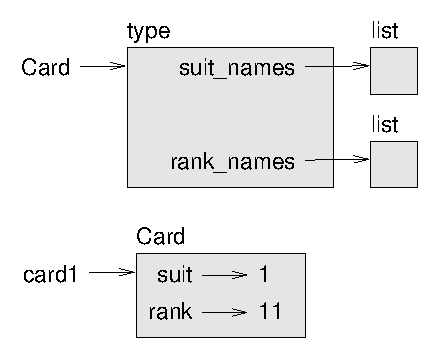
\includegraphics[scale=0.8]{figs/card1.eps}}
\caption{オブジェクト図}
\label{fig.card1}
\end{figure}
%
\section{カードの比較}
組み込み型に関しては比較演算子（{\tt <},{\tt >},{\tt ==},etc）がより大きい、より小さい、他と等しいなどの値の比較に使える。
ユーザ定義型については、``less than"を意味する{\verb"__lt__"}メソッドが提供する組み込み型の操作を再定義することになる。\par
メソッド{\verb"__lt__"}は二つの引数{\tt self}と{\tt other}を受け取り、
{\tt self}が{\tt other}未満であると{\tt Ture}を返す。\par
カードの順位は自明ではない。
例えば、クラブの3とダイアモンドの2ではどちらが上か？
一つは高いランクを持つが、他はスートでは上である。比較を可能にするためには、ランクとスートのどちらが重要かを決めないといけない。
多分この答えは実際のゲームのルールによる。しかし、ここでは問題を簡単にするために、
スートはより重要だと恣意的だが設定しよう。従って、スペードの全てのカードはどんなダイアモンドより高位になる、そして以下同様である。\par
このように決めると比較演算子のメソッド{\verb"__lt__"}を書くことができる。
\begin{verbatim}
# クラスCardの定義に中で:

    def __lt__(self, other):
        #  まずスートを調べる
        if self.suit < other.suit: return True
        if self.suit > other.suit: return False

        # スートは同じなので、ランクを調べる
        return self.rank < other.rank
\end{verbatim}
タプルの比較を用いるともっと簡便に書ける：
\begin{verbatim}
# クラスCardの定義に中で:

    def __lt__(self, other):
        t1 = self.suit, self.rank
        t2 = other.suit, other.rank
        return t1 < t2
\end{verbatim}
(訳注：ここの演算子{\tt <}はタプルに定義されている比較演算子である。）\par
練習問題として、{\tt Time}オブジェクトのための{\verb"__lt__"}メソッドを書け。
タプルの比較を用いることでもよいが、整数の引き算を使うこともできる。
%
\section{積み札}
カードの定義が終わったので、次は積み札の定義である。
積み札は複数のカードからなるので、カードのリストを属性に持つことは自然なことである。
以下は{\tt Deck}クラスの定義である。
{\tt init}メソッドでは属性{\tt cards}を生成、ここでは52枚の標準カードを持たせた。
\begin{verbatim}
class Deck:

    def __init__(self):
        self.cards = []
        for suit in range(4):
            for rank in range(1, 14):
                card = Card(suit, rank)
                self.cards.append(card)
\end{verbatim}
カードの山を作成する最も安易な方法は入れ子のループを使うことだ。
外側のループは0から3までスートを列挙し、内側のループは1から13までランクを列挙している。
繰り返し毎に新しいカードが生成され、{\tt self.cards}に追加される。
%
\section{積み札のプリント}
{\tt Deck}のための{\verb"__str__"}メソッドは以下のようになる：
\begin{verbatim}
# クラスDeckの定義に中で
    def __str__(self):
        res = []
        for card in self.cards:
            res.append(str(card))
        return '\n'.join(res)
\end{verbatim}
このメソッドは大きな文字列を纏める有効な方法を示している。
つまり、文字列のリストを作り、{\tt join}を使い纏める。
カードに対する組み込み関数{\tt str}はカード毎にその{\verb"__str__"}メソッドを発動させ、
文字列の表現を返す（訳注：{{\tt Card}オブジェクトで定義された\verb"__str__"}メソッドは関数{\tt str(card)}でも発動される）。
{\tt join}メソッドは改行文字で発動されているので、各カードは一行毎にプリントされる。以下は結果である：
\begin{verbatim}
>>> deck = Dec()
>>> print deck
Ace of Clubs
2 of Clubs
3 of Clubs
………
10 of Spades
Jack of Spades
Queen of Spades
King of Spades
\end{verbatim}
結果は52行の表示であるが、これは改行文字を含む一つの長い文字列である。
%
\section{追加・移送・シャッフル・ソート}
カードの扱いとして欲しいメソッドとしては、カードの山から一枚のカードを移送する、及び追加するがある。\par
第一のメソッドに対して、{\tt pop}が便利な方法を提供できる：
\begin{verbatim}
# クラスDeckの定義に中で
    def pop_card(self):
        return self.cards.pop()
\end{verbatim}       
{\tt pop}はリストの最後の要素を削除するので、積み札の底からカードを抜き取ることになる。
実際のゲームでは「底から抜き取り」は眉をひそめる行為であるが、今の場合はよしとする。\par
カードの追加は{\tt append}を使う：
\begin{verbatim}
# クラスDeckの定義に中で
    def add_card(self, card):
        self.cards.append(card)
\end{verbatim}
このような大したこともしないで他の関数を使うメソッドは{\bf ベニヤ（veneer）}と呼ばれる。
これは良質の木材の薄い層を張り合わせて廉価な木材を作り出す木工技術の比喩からきている。
ここでは積み札に対して妥当なリストの処理を「薄い」メソッドとして定義している。\par
シャッフルも同様にして、{\tt random}モジュールの{\tt shuffle}関数を使って{\tt shuffle}メソッドを{\tt Deck}の内部に作る：
\begin{verbatim}
# クラスDeckの定義に中で
    def shuffle(self):
        random.shuffle(self.cards)
\end{verbatim}
randomモジュールのインポートを忘れないように。\par
練習問題として、{\tt Deck}のもう一つのメソッド{\tt sort}をリストのメソッド{\tt sort}を使って作成せよ。
メソッド{\tt sort}はソートの順位を決めるために{\tt Card}オブジェクトの{\verb"__lt__"}メソッドを使う。
%
\section{継承}
継承は既存のクラスを改変することで新しいクラスを生成する能力のことだ。
新しいクラスは既存のクラスのメソッドを引き継ぐので、これは「継承」と呼ばれている。
この比喩を拡張して、既存のクラスは{\bf 親クラス（parent class）}、新しいクラスは{\bf 子クラス（child class）}と呼ばれる。 \par
例として、一人のカードプレーヤが保持しているカード、つまり手札を考えてみよう。手札は積み札に似ている。
どちらもカードの集合からなっていて、追加や移送の操作を必要とする。\par
手札は積み札と異なる面もある。積み札では意味を成さないような操作が手札については必要になることがある。
例えば、ポーカーではどちらが勝者かを決めるために二人の手札を比較する必要がある。
また、ブリッジでは賭けをするために、手札のスコアを計算する必要がある。 \par
このようなクラス間の異同はそれ自体で継承という概念に繋がっている。
子のクラスの定義は他のクラスの定義と似ているが、親クラスの名前が括弧の中に入る：
\begin{verbatim}
class Hand(Deck):
    """Represents a hand of playing cards."""
\end{verbatim}
この定義では{\tt Hand}クラスは{\tt Deck}を継承している。
つまり、{\tt Deck}クラスのメソッド{\tt pop\_card}や{\tt add\_card}が{\tt Hand}でも使えるわけだ。
{\tt Hand}は{\tt Deck}クラスの{\verb"__init__"}メソッドも継承できるが、それは欲しいものではない。
52枚のカードを手札とする替わりに{\tt init}メソッドは空のリストで始めることが似つかわしい。
以下は{\tt Hand}クラスの{\tt init}メソッドであるが、これは{\tt Deck}クラスのそれを再定義することになる：
\begin{verbatim}
# クラスHandの定義に中で
    def __init__(self, label=''):
        self.cards = []
        self.label = label
\end{verbatim}
従って、一つの手札を生成するときにはPythonはこの{\tt init}メソッドを発動する：
\begin{verbatim}
hand = Hand('new hand')
print(hand.cards)
[]
print(hand.label)  #訳注：属性label（単なる文字列）の印刷
new hand
\end{verbatim}
しかし、その他のメソッドは継承するので、{\tt pop\_card}や{\tt add\_card}はここでも使える：
\begin{verbatim}
>>> deck = Deck()
>>> card = deck.pop_card()
>>> hand.add_card(card)
>>> print(hand)  #訳注Handクラスのインスタンスhandそのものの印刷
King of Spades
\end{verbatim}
この手続きを{\tt Deck}のメソッド{\tt move\_card}としてカプセル化することは自然なことである：
\begin{verbatim}
# クラスDeckの定義に中で
    def move_cards(self, hand, num):
        for i in range(num):
            hand.add_card(self.pop_card())
\end{verbatim}
{\tt move\_cards}は引数を二つ持ち、一つは{\tt Hand}オブジェクトそして操作するカードの枚数{\tt num}である。
このメソッドは{\tt self}も{\tt hand}を修正し、戻り値は{\tt None}であることに注意。\par
カードゲームのいくつかではカードの移動は手札から手札、
手札から積み札へ戻すなどがあるが、この{\tt move\_cards}を使えばよい。
{\tt self}は{\tt Deck}でも{\tt Hand}でもよい。更に仮引数は{\tt hand}となっているけれど、これは{\tt deck}でもよい。\par
継承は有用な機能だ。継承なしては繰り返しになってしまうプログラムも継承によって綺麗にかけることがある。
継承は親クラスを変更することをしないでも親クラスの振る舞いをカスタマイズできるので、コードの再利用の機能を果たす。
あるケースでは、継承は問題自体が持つ性質を反映することがあり、プログラムをより読みやすくする。
一方、継承はプログラムを読みにくくすることもある。あるメソッドが発動されたとき、その定義がどこにあるのかが明白でないこともある。
関連するコードがいくつかのモジュールに渡って散乱していることもあるうる。継承を使ってなし得る多くのことがそれ無しでも充分にやれることもある。
%
\section{クラス図}
これまでプログラムの状態を示すスタック図、オブジェクトの属性とそれらの値の関係を示したオブジェクト図をみてきた。
これらの図はプログラム進行中のスナップショットであり、プログラムの進行に連れて変わる。
それらは極めて詳細を究め、ある目的には詳細過ぎる。{\bf クラス図（class diagram）}はプログラムの構造をより抽象的に表現したものである。
個々のオブジェクトを示すかわりに、クラスとクラス間の関係を示す。\par
複数のクラスの間にある関係としては以下のものがあり得る：
\begin{itemize}
\item 一つのクラス・オブジェクトが他のクラスのオブジェクトの参照を含む。
例えば、個々の{\tt Rectangle}オブジェクトは{\tt Point}オブジェクトの参照を含んでいるし、
個々のDeckオブジェクトは多くのCardオブジェクトの参照を含んでいる。
この関係は「一つの{\tt Rectangle}は一つの{\tt Point}を持っている」にあるように{\bf HAS-A関係（HAS-A relationship）}と呼ぶ。
\item 一つのクラスが他のクラスを継承する。この関係は「HandはDeckの一種である」にあるように{\bf IS-A関係（IS-A relationship）}と呼ぶ。
\item 一つのクラスの変更が他のもう一つのクラスの変更を要求するといった依存関係にある二つのクラス間の関係。
\end{itemize}
クラス図はこれらの関係を図式したものだ。例えば、図\ref{fig.class1}は{\tt Card}、{\tt Deck}、{\tt Hand}間の関係を示したものだ。
% 
\begin{figure}[htbp]
\centerline
{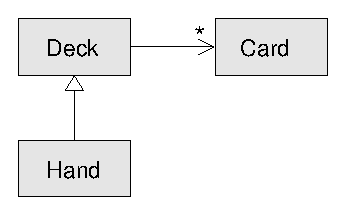
\includegraphics[scale=0.8]{figs/class1.eps}}
\caption{クラス図}
\label{fig.class1}
\end{figure}
%
白抜きの矢印は{\tt IS-A}の関係を表示している。
この図では{\tt Hand}は{\tt Deck}を継承していることを示している。
普通の矢印は{\tt HAS-A}の関係を表示している。
この図では{\tt Deck}は{\tt Card}の参照を持っていることを示している。
矢印の上部のスター（{\tt *}）は{\bf 重複度（multiplicity）}である。
これは{\tt Deck}クラスには何個の{\tt Card}オブジェクトの参照があるかを表示するものである。
これは単に52といった単なる数字、5..7と言った区間、任意の数を示すスターなどでよい。
この図では{\tt Deck}は任意の数のカードを持ち得るのでスターになっている。\par
この図では依存関係は何もない（訳注：「依存関係」の説明は語句の
{\bf 依存関係（dependency）}をみよ）。依存関係があるとこれは破線の矢印で示すか、沢山の依存関係があるときには
それらは省略される。\par
もっと詳細に渡る図にしようとすれば、{\tt Deck}オブジェクトはカードのリストを含んでいることを示すことになるが、
クラス図にはリスト、辞書などの組み込み型は含めない。
%
\section{デバッギング}
継承はあるオブジェクトのあるメソッドの発動がどちらのメソッドの発動か不明であるということがあるので、デバッグは新たな問題をはらんでくる。\par
いまHandオブジェクトに付随した関数を書こうとしたとする。その関数はポーカーの手札、ブリッジの手札だといったどのような手札でも有効したいと思ったとしよう。
こうなると、例えば{\tt shuffl}eというメソッドを発動させたときに、
{\tt Deck}で定義されたものか、そのサブクラスで再定義されたものの１つかということになる。
このように、どのメソッドが発動されたか不確かになってしまう。この簡単な解決法は当該のメソッドの先頭に{\tt print}文を追加しておくことだ。
もし{\tt Deck.shuffle}が発動されると、{\tt 'Running Deck.shuffle'}とメッセージが出るわけである。これで実行の流れが追跡できる。\par
別な方法はオブジェクトとメソッド名（文字列）を引数に取り、そのメソッドを定義しているクラスを返す以下の関数を使うことだ：
\begin{verbatim}
def find_defining_class(obj, meth_name):
    for ty in type(obj).mro():
        if meth_name in ty.__dict__:
            return ty
例だ：
>>> hand = Hand()
>>> find_defining_class(hand, 'shuffle')
<class 'Card.Deck'>　（訳注：モジュール名がCardの場合である）
\end{verbatim}
従って{\tt  Hand}の{\tt shuffle}メソッドはクラス{\tt Deck}で定義されたものを使っていることが分かる。
関数{\tt find\_defining\_class}ではメソッドが探索される
クラスのリストを得るメソッド{\tt mro}が使われている（``MRO"は``method resolution order"の略である）。\par
以下はプログラム設計に際しての示唆である。何らかの理由でメソッドを書き換える必要があるときにはいつでも、
そのインタフェースは古いものと同じにすべきである。同じ型の仮引数で、戻り値も同じ型にする。
つまり、同じ事前条件と同じ事後条件に従うようにする。この条件に従ってプログラムを設計すると、
上位クラス（例えば{\tt Deck}）のインスタンスで有効な関数を作っておくと、
この関数はそのサブクラス（例えば{\tt Hand}や{\tt PokerHand）}のインスタンスでも有効に使えることになる。
このルール（リスコフ({\it Liskov})の置換原理）に違反すると、そのコードはカードで作った家のように簡単に崩壊する。
%
\section{データカプセル化}
前章では「オブジェクト指向設計」とも呼ぶべきプログラム開発設計の過程を示した。
まず必要な実体、{\tt Time}、{\tt Point}、{\tt Rectangle}を確定した。そして、これらを表現するためのクラスを定義した。
各々において、オブジェクトと現実世界の実体との明白な対応関係（少なくとも数学的世界の）がある。\par
しかし、どうようなオブジェクトが必要で、それらがいかに相互作用するのかが明白でない場合も往々にしてある。
このような場合には別の方法を取る必要がある。関数のインタフェースはカプセル化や一般化の原則の実現体であるように、
クラスのインタフェースも{\bf データカプセル化（data encapsulation）}の原則を実現したものにすべきだ。\par
13.8節で議論したマルコフ解析はよい実例を提供してくれる。 \\
\url{https://thinkpython.com/code/markov.py}をダウンロートしてそのコードを眺めると、
いくつかの関数から読み書きされる二つの大域変数{\tt suffix\_map}と{\tt prefix}とが定義されている：
\begin{verbatim}
suffix_map = {}
prefix = ()
\end{verbatim}
これらの変数は大域変数であるので、一度に一つのテキストの解析ができるだけである。
もし二つのテキストを同時に解析するとなると、同じデータ構造に追加することになる（これ自体は興味のある結果を生むが）。
複数の解析を別々なデータ構造に収めようとすると、各解析の状態を一つのオブジェクトにカプセル化する必要がある。それは以下のようになる：
\begin{verbatim}
class Markov:
    def __init__(self):
         self.sufix_map = {}
         self.prefix = ()
\end{verbatim}
次ぎに関数をメソッドに変換する。例として、{\tt process\_word}関数を変換してみる：
\begin{verbatim}
    def process_word(self, word, order=2):
        if len(self.prefix) < order:
            self.prefix += (word,)
            return

        try:
            self.suffix_map[self.prefix].append(word)
        except KeyError:
            # if there is no entry for this prefix, make one
            self.suffix_map[self.prefix] = [word]

        self.prefix = shift(self.prefix, word)        
\end{verbatim}
関数の中味を変えずにデザインを変える手法はプログラムの変更方法に対する再因子分解のもう一つの事例である（4.7節）。\par
この例はオブジェクトやメソッドをデザインするための開発計画を示唆している：
\begin{enumerate}
\item まず、大域変数（もし必要なら）を使って読み・書きする関数を書く。
\item そのプログラムが動くようになったら、それらの大域変数とそれらを使う関数の関係を探す。
\item 関連する変数を一つのオブジェクトの属性としてカプセル化する。
\item 付随する関数は新たなクラスのメソッドになるように変換する。
\end{enumerate} 
練習問題として、\url{https://thinkpython.com/code/markov.py}をダウンロードし、
上記のステップに従い大域変数を新たなクラス{\tt Markov}の属性としてカプセル化せよ。\\
解答例：\url{https://thinkpython.com/code/Markov.py}（大文字の{\tt M}に注目）。
%
\section{語句}

\begin{description}

\item[符号化（encode）：] 二つの集合の対応関係を構築することによって一つ値の集合を他の値の集合で表現する。
%\index{encode}

\item[クラス属性（class attributes）：] クラスオブジェクトに属する属性。クラス属性はクラスの定義の中で定義されるが
如何なるメソッドの外側に置く。
%\index{class attribute}
%\index{attribute!class}

\item[インスタンス属性（instance attributes）：] クラスのインスタンスに属する属性。
%\index{instance attribute}
%\index{attribute!instance}

\item[ベニヤ（veneer）：] 大した計算過程も無く他の関数に異なったインターフェースを提供するメソッドや関数。
%\index{veneer}

\item[継承（inheritance）：] 既存のクラスの改訂版になるような新しいクラスを定義する能力。
%\index{inheritance}

\item[親クラス（parent class）：] それから子クラスが派生する元のクラス。
%\index{parent class}

\item[子クラス（child class）：] 既存のクラスから派生して作られた新しいクラス。「下位クラス」とも呼ばれる。
%\index{child class}
%\index{class!child}

\item[IS-A 関係（IS\_A relationship）：] 子クラスとその親クラスといった関係。
%\index{IS-A relationship}

\item[HAS-A関係 （HAS\_A　relationship）：] 二つのクラスで一つクラスのインスタンスが他のクラスのインスタンスへの参照を含む
ような関係。
%\index{HAS-A relationship}

\item[依存関係（dependency）：] 一つのクラスのインスタンスが他のインスタンスへの参照を含むような二つのクラスの関係。
%\index{dependency}

\item[クラス図（class diagram）：] 一つのプログラムの中に現れるクラスとそれらの間の関係を示すグラフィカルな表現。
%\index{class diagram}
%\index{diagram!class}

\item[重複度（multiplicity）：] HAS-A関係の関係にある二つのクラスで他のクラスののインスタンスへの参照が何回あるかを示す表示法。
%\index{multiplicity}

\item[データカプセル化（data encapsulation）:] プログラムの原型で使っていた大域変数を最終版ではインスタンス属性にして
隠すプログラム開発法。
%\index{data encapsulation}

\end{description}
%
\section{練習問題}

\noindent
{\bf 練習問題\tp.1} 以下のようなプログラムに対してクラスやこのクラスの間の関係を示す{\tt UML}クラス図を作成せよ。
（訳注：統一モデリング言語（{\tt UML}）によるクラス図は本文の図\ref{fig.class1}で表示されているクラス図と思えばよい。この
練習問題では「依存関係」もあることに注意。）

\begin{verbatim}
class PingPongParent:
    pass

class Ping(PingPongParent):
    def __init__(self, pong):
        self.pong = pong


class Pong(PingPongParent):
    def __init__(self, pings=None):
        if pings is None:
            self.pings = []
        else:
            self.pings = pings

    def add_ping(self, ping):
        self.pings.append(ping)

pong = Pong()
ping = Ping(pong)
pong.add_ping(ping)
\end{verbatim} \par

\noindent
{\bf 練習問題\tp.2} 以下はポーカーの可能な手を値打ちの少ない順序（従って確率の大きな順序）に並べたものである：
\begin{description}

\item[pair:] 同じランクを持った二枚のカード
\vspace{-0.05in}

\item[two pair:] 同じランクを持った二枚のカードの二組
\vspace{-0.05in}

\item[three of a kind:] 同じランクを持った三枚のカード
\vspace{-0.05in}

\item[straight:] 引き続くランクからなる五枚のカード（エースは高くも低くにもなれる。
従って、Ace-2-3-4-5はstraight、10-Jack-Queen-King-Aceもstraight、
しかし、Queen-King-Ace-2-3はstraightではない）
\vspace{-0.05in}

\item[flush:] 同じスートの五枚のカード
\vspace{-0.05in}

\item[full house:] 一つのランクの三枚のカードと他のランクの二枚のカード
\vspace{-0.05in}

\item[four of a kind:] 同じランクの四枚のカード
\vspace{-0.05in}

\item[straight flush:] 同じスートで引き続くランク（上で定義したように）からなる五枚のカード
\vspace{-0.05in}

\end{description}

さてこの練習問題の目標は上のような手を引き当てる確率を推定することにある。
\begin{enumerate}
\item 以下のファイルを\url{https://thinkpython.com/code}からダウンロードせよ。
{\tt Card.py} ：これは{\tt Card}、{\tt Deck}、{\tt Hand}のクラス記述の完全版である。\\
{\tt PokerHand.py} ：ポーカーの手を表現するためのクラスの不完全な記述とそのテストコードである。
\item {\tt PokerHand.py}を起動すると ``7-card"ポーカーの七枚の手札が配られ、
この手札にflushが含まれているかをチェックするようになっている。
\item {\tt PokerHand}に{\tt has\_pair}、{\tt has\_twopair}というメソッドを追加せよ。
これらのメソッドは手札に当該の手が含まれていると{\tt True}を、そうでなければ{\tt False}を返す。
コードは任意の枚数の手札でも手を検出できること（5とか7とかがよくある数であるが）。
\item 一つの手札に含まれる最高位の手を調べる{\tt classify}メソッドを作成せよ。
そして属性の{\tt label}をそれに従ってセットせよ。例えば、``7-card"の手としてflushを含んでいたら、
'{\tt flush'}という文字列を{\tt label}に代入する。
\item この{\tt classify}メソッドが動くことが確認できたら、
次ぎのステップは種々の手の確率を求める番だ。{\tt PokerHand.py}内に積み札をシャッフルしてそれを手札に分割し、
各手札を{\tt classify}で分類し、特定の分類値が起こる回数を調べる関数を書け。
\item 分類値とその確率を表にしてプリントせよ。
充分長く実行して沢山の手を発生させその確率が適当な桁で落ち着くまでプログラムを実行せよ。
結果を\url{http://en.wikipedia.org/wiki/Hand_rankings}と比較せよ。
\end{enumerate}
解答例： \url{https://thinkpython.com/code/PokerHandSoln.py}.
%
\chapter{便利グッズあれこれ}
この本の目的は最小限の範囲でPythonを学習できるようにすることである。それ故何か行う上で二つの方法
があるときには、１つだけを取り上げ他は伏せてきた。ときとして二番目の方法は練習問題に含めてきた。\par
この章ではこれまで取り上げなかった便利グッズの幾つかについて触れることにしたい。Pythonは必ずしも
必要としない「呼び物」を幾つか提供している。それら無しで優れたコードを書くことができるが、ときとして
それらを使うと、すっきりして、読みやすく、効率のよい、時としてこの三つを兼ね揃えたコードを書くことが
できる。
%
\section{条件付き表式}
条件文については5.4節でみた。条件文は二つの値の内一つを選択するケースでよく
用いられる。例を上げると：
\begin{verbatim}
if x > 0:
    y = math.log(x)
else:
    y = float('nan')
\end{verbatim}
この文では{\tt x}が正の値か調べる。そうであると{\tt math.log}が実行される。そうでないと
{\tt math.log}は{\tt ValueError}の例外を発生してしまう。これを避けるために、ここでは
``NaN"を生成する。これは``Not a Number"の意味の特別な浮動小数点値である。\par
さてこれを{\bf 条件付き表式（conditional expression）}で書くと以下のようによりすっきりと書ける：
\begin{verbatim}
y = math.log(x) if x > 0 else float('nan')
\end{verbatim}
これは英語を読むように読める：
 ``{\tt y} gets log-{\tt x}
if {\tt x} is greater than 0; otherwise it gets NaN''.　\par
再帰関数もこの条件付き表式を使って書き直すことができる。例として{\tt factorial}関数
の再帰版を取り上げる。元のコードは：
\begin{verbatim}
def factorial(n):
    if n == 0:
        return 1
    else:
        return n * factorial(n-1)
\end{verbatim}
これを書き直すと：
\begin{verbatim}
def factorial(n):
    return 1 if n == 0 else n * factorial(n-1)
\end{verbatim}
となる。\par
もう一つの利用法は選択的引数の処理である。例として
練習問題17.2の{\tt GoodKangaroo}の{\tt init}メソッドを取り上げる。
元は：
\begin{verbatim}
    def __init__(self, name, contents=None):
        self.name = name
        if contents == None:
            contents = []
        self.pouch_contents = contents
\end{verbatim}
書き直すと
\begin{verbatim}
    def __init__(self, name, contents=None):
        self.name = name
        self.pouch_contents = [] if contents == None else contents 
\end{verbatim}
となる。\par
一般に条件分岐の両方が{\tt return}文とか同じ変数への代入とかの簡単な表式であるときには
条件文を条件付き表式に置き換えることができる。
%
\section{リスト内包}
10.7節で写像とフィルターのコードパターンで考察した。例えば以下の関数は文字列のリスト
を引数として文字列の組み込みメソッド{\tt capitalize}を各要素に適用し新たなリストを戻す：
\begin{verbatim}
def capitalize_all(t):
    res = []
    for s in t:
        res.append(s.capitalize())
    return res
\end{verbatim}
これを{\bf リスト内包（list comprehension）}を使って書き直すと：
\begin{verbatim}
def capitalize_all(t):
    return [s.capitalize() for s in t]
\end{verbatim}
となる。角括弧の演算子があることから新たなリスト作成であることが分る。
この角括弧の中の表式はリストの要素を表現し、{\tt for}節がどのような
配列を横断的に処理するのか示している。\par
リスト内包の構文は変数{\tt s}が定義する前に表式に現われるので少し不恰好である。\par
リスト内包はデータフィルタリングでも使うことができる。以下はリスト{\tt t}から大文字だけでできている
文字列の要素を選択し新たなリストを作る関数である：
\begin{verbatim}
def only_upper(t):
    res = []
    for s in t:
        if s.isupper():
            res.append(s)
    return res
\end{verbatim}
これを書き直すと：
\begin{verbatim}
def only_upper(t):
    return [s for s in t if s.isupper()]
\end{verbatim}
となる。\par
リスト内包表現はコンパクトで{\tt for}ループによる同等のものより速く、あるばあいには
ずっと速い。それならばもっと早いところでこれに触れてほしかったとあなたは苦情を言う
かもしれないが、それは予想していたことである。\par
言い訳になるが、リスト内包表現はループの中に{\tt print}文を入れることができないのでデバック
が困難になる難点がある。リスト内包は計算が最初から明白に正しいことがわかっているような
十分に単純なばあいに使うとよい。こんなことは初心者ではないはずだ。
%
\section{ジェネレータ表式}
ジェネレータ表式（generator expressions）はリスト内包に似ているが、角括弧の替わりに
括弧を使う：
\begin{verbatim}
>>> g = (x**2 for x in range(5))
>>> g
<generator object <genexpr> at 0x7f4c45a786c0>
\end{verbatim}
結果は値の配列を通じて如何に繰り返しの演算をするか表現したジェネレータ・オブジェクト
である。しかしリスト内包と異なり、一時に値の計算をすることをしない。問い合わせがあるまで
待っている。組み込み関数{\tt next}がこのジェネレータから次の値を得るのに使われる：
\begin{verbatim}
>>> next(g)
0
>>> next(g)
1
\end{verbatim}
配列の最後の到達すると、{\tt next}関数は{\tt StopIteration}例外を吐き出す。
値を{\tt for}ループで繰り返し取り出す処理でも使える：
\begin{verbatim}
>>> for val in g:
...     print(val)
4
9
16
\end{verbatim}
ジェネレータ・オブジェクトは常に配列の何処にいるかを追尾している{\tt for}ループ
は{\tt next}が抜け出たところを取り出す。ジェネレータを使い切ると、それ以降は
{\tt StopIteration}例外を吐き出す：
\begin{verbatim}
>>> next(g)
StopIteration
\end{verbatim}
ジェネレータ表式は{\tt sum}、{\tt max}そして{\tt min}といった関数と一緒に使われることが多い：
\begin{verbatim}
>>> sum(x**2 for x in range(5))
30
\end{verbatim}
%
\section{{\tt any}と{\tt all}}
Pythonはブーリアン値を要素とする配列を受け取りそれらの値に一つでも{\tt Ture}があると
{\tt Ture}を返す組み込み関数{\tt any}を提供している。これはリストに対して動作する：
\begin{verbatim}
>>> any([False, False, True])
True
\end{verbatim}
この関数はジェネレータ表式と一緒に使われることが多い：
\begin{verbatim}
>>> any(letter == 't' for letter in 'monty')
True
\end{verbatim}
この例題では{\tt in}演算子と同じことをするだけなので有難味がない。
しかし9.3節で展開したような探索関数の幾つかはこの{\tt any}を使って
書き直すことができる。例えば{\tt avoids}は以下のようになる。：
\begin{verbatim}
def avoids(word, forbidden):
    return not any(letter in forbidden for letter in word)
\end{verbatim}
この関数はほぼ英文を読むように書けている：``{\tt word} avoids
{\tt forbidden} if there are not any forbidden letters in {\tt word}.''\par
関数{\tt any}をジェネレータ表式と合わせて使うことは{\tt any}が{\tt Ture}
を検出したらジェネレータは停止するので効率がよい。全ての配列を評価
しないで済む。\par
Pythonはもう一つの組み込み関数{\tt all}を提供している。この関数は
配列の要素全てが{\tt Ture}のとき{\tt Ture}を返す。練習問題として
9.3節の{\tt uses\_all}をこの関数を使って書き直せ。
%
\section{セット}
13.6節では文書に出現したが単語のリストにはない単語を見つける問題に出会った。
そこで作成した関数は文書から出現した単語をキーとする辞書{\tt d1}
と単語のリストを含む辞書{\tt d2}を引数とした。その関数の戻り値も辞書で
{\tt d1}にあって{\tt d2}のない単語をキーとしたものであった。つまり：
\begin{verbatim}
def subtract(d1, d2):
    res = dict()
    for key in d1:
        if key not in d2:
            res[key] = None
    return res
\end{verbatim}
これら辞書では値は全て{\tt None}であった。これは記憶領域を無駄
にしている。\par
Pythonは{\tt set}と呼ばれる組み込み型を提供している。これは
辞書に似ているがキーの集合で値を持たない。セットへの要素の
追加は高速で、要素の検索を速い。
そしてよく知られた集合演算を実行するメソッドや関数が提供
されている。
例えば集合の差を求めるためには{\tt difference}というメソッドか
減算演算子{\tt -}を使えばよい。これを使えば
{\tt subtract}は以下のように書ける：
\begin{verbatim}
def subtract(d1, d2):
    return set(d1) - set(d2)
\end{verbatim}
戻り値は辞書でなく、セットである。しかし繰り返しのような操作
は振る舞いは同じである。\par
この本の練習問題の幾つかはこのセットを使うとコンパクトで
効率のよいものに書き直すことができる。
例えば、辞書を使った練習問題10.7の関数{\tt has\_duplication}の
解答例は：
\begin{verbatim}
def has_duplicates(t):
    d = {}
    for x in t:
        if x in d:
            return True
        d[x] = True
    return False
\end{verbatim}
であるが、これは要素がはじめて現れたものであるとそれは辞書に追加
され、同じ要素が現れると関数は{\tt Ture}を戻り値として終了する。\par
これをセットを使って書き直すと：
\begin{verbatim}
def has_duplicates(t):
    return len(set(t)) < len(t)
\end{verbatim}
一つの要素はセットでは一回のみである。だから配列で同じ要素が二回
以上現れるとそのセットの大きさは配列{\tt t}より小さくなる。配列
{\tt t}の重複がなければ、そのセットの大きさは配列の大きさと同じいなる。\par
第9章の練習問題の幾つかもセットで書き直すことができる。例えば
関数{\tt use\_only}を取り上げてみよう：
\begin{verbatim}
def uses_only(word, available):
    for letter in word: 
        if letter not in available:
            return False
    return True
\end{verbatim}
この関数は文字列{\tt word}の中の全ての文字が文字列{\tt available}
の中にあるものか調べている。書き直すと：
\begin{verbatim}
def uses_only(word, available):
    return set(word) <= set(available)
\end{verbatim}
演算子{\tt <=}は一つのセットが他のサブセット（それらが等しいことも含めて）
であるかどうかを調べる。だから{\tt word}のセットが{\tt available}の
サブセット（または等しい）と{\tt Ture}を返す。\par
練習問題として、関数{\tt avoids}をセットを使って書き直せ。
%
\section{カウンター}
カウンターは要素の重複を許すことを除けばセットに似ている。カウンターはその要素が
何回現れたを常に追跡している。数学の{\bf 多重集合（multiset）}の概念に馴染み
があればカウンターは多重集合を表現する自然な方法である。\par
{\tt Counter}は標準モジュール{\tt collections}の中に納められているのでそれを
インポートする必要がある。カウンターの初期化は文字列、リスト等
繰り返しの操作を伴なう型データで行う：
\begin{verbatim}
>>> from collections import Counter
>>> count = Counter('parrot')
>>> count
Counter({'r': 2, 't': 1, 'o': 1, 'p': 1, 'a': 1})
\end{verbatim}
カウンターは辞書のように振舞う。各々のキーはそれが何回出現したという回数に
写像される。辞書の同じく、キーはハッシュ可能でなければならない。\par
辞書と異なり、存在しないキーにアクセスしようとしても例外を発生しない。替わりに
{\tt 0}を返す。
\begin{verbatim}
>>> count['d']
0
\end{verbatim}
練習問題10.6の{\tt is\_anagram}はこのカウンターを使うとコンパクトに書ける：
\begin{verbatim}
def is_anagram(word1, word2):
    return Counter(word1) == Counter(word2)
\end{verbatim}
もしも二つの単語がアナグラムであると、それらは同じ文字を同じ回数で含んでいるはずである。
それらのカウンターは同等であるはずだ。\par
カウンターは集合の加法、減法、合同、交差などの集合の演算を実行するメソッドや関数を
提供している。そして中でも有用な{\tt most\_common}メソッドがある。これはカウンターの要素
を最大頻度順でソートした値ー頻度の対を要素としたリストを返すメソッドである。
\begin{verbatim}
>>> count = Counter('parrot')
>>> for val, freq in count.most_common(3):
...     print(val, freq)
r 2
p 1
a 1
\end{verbatim}
%
\section{デフォルト辞書}
モジュール{\tt collections}は辞書に似ているが存在しないキーにアクセスしようとすると例外ではなく
その場で新たに新規の値を作ることができる{\tt defaultdict}を提供している。\par
{\tt defaultdict}を作るとき新しい値を如何に作るかを示す関数を合わせて指定する。この関数
をときとしてファクトリー{\tt factory}と呼ぶ。リスト、セットそして他の型のデータを作りだす組み込み
関数がファクトリーとして使える。
\begin{verbatim}
>>> from collections import defaultdict
>>> d = defaultdict(list)
\end{verbatim}
ここで引数が空のリストを作る関数{\tt list()}ではなくクラスオブジェクトの{\tt list}であることに注意。
提供した関数は存在しないキーへのアクセスがあるまで呼ばれることはない：
\begin{verbatim}
>>> t = d['new key']
>>> t
[]
\end{verbatim}
{\tt t}と呼ばれている新しいリストがこのキーと対になる値として辞書に追加される。それ故に
{\tt t}を修正すると、この修正はこの辞書に反映される：
\begin{verbatim}
>>> t.append('new value')
>>> d
defaultdict(<class 'list'>, {'new key': ['new value']})
\end{verbatim}
リストを値として持つような辞書の作成に絡む問題ではこのデフォルト辞書を使うとより簡単
にコードを書くことができる。練習問題12.2（解答例：\url{https://thinkpython.com/code/anagram_sets.py}）
では文字をソートした一つの文字列をそれらの文字から作られる単語のリストの写像する辞書を作る問題だった。
例えば、 {\tt opst'}はリスト{\tt ['opts', 'post', 'pots', 'spot', 'stop', 'tops']}に写像される。
元のコードは
\begin{verbatim}
def all_anagrams(filename):
    d = {}
    for line in open(filename):
        word = line.strip().lower()
        t = signature(word)
        if t not in d:
            d[t] = [word]
        else:
            d[t].append(word)
    return d
\end{verbatim}
（訳注：ここで関数{\tt signature}は単語{\tt word}を受け取りその中の文字をアルファベット
順に並び替えた文字列を戻す。） \par
この例題は{\tt setdefualt}を使うと簡単化できる（これは練習問題11.2）：
\begin{verbatim}
def all_anagrams(filename):
    d = {}
    for line in open(filename):
        word = line.strip().lower()
        t = signature(word)
        d.setdefault(t, []).append(word)
    return d
\end{verbatim}
この解等はそれが必要であるかどうかに拘わらず毎回新たなリストを作るという欠点がある。
リストではこれは大きな問題ではないが、ファクトリー関数が複雑になると問題になるかも
しれない。\par
{\tt defaultdict}を使うとこの問題を避けることができる：
\begin{verbatim}
def all_anagrams(filename):
    d = defaultdict(list)
    for line in open(filename):
        word = line.strip().lower()
        t = signature(word)
        d[t].append(word)
    return d
\end{verbatim}
練習問題18.3の解答例（\url{https://thinkpython.com/code/PokerHandSoln.py}）
では{\tt has\_straightflush}関数で{\tt setdefault}を使っていた。
この解は必要の如何に拘わらずループの繰り返しごとに{\tt Hand}オブジェクトを生成すると
いった欠点を持っていた。練習問題として、その関数を{\tt defaultdict}を使って書き直せ。
%
\section{名前付きタプル}
多くの単純なオブジェクトは基本的に関連性のあるデータの集合である。例えば
第15章の{\tt Point}オブジェクトは二つの数値{\tt x}と{\tt y}を属性として
持っている。このようなクラスを定義するときには、一般的には{\tt init}メソッド
と{\tt str}メソッドで初めてきた：
\begin{verbatim}
class Point:

    def __init__(self, x=0, y=0):
        self.x = x
        self.y = y

    def __str__(self):
        return '(%g, %g)' % (self.x, self.y)
\end{verbatim}
これは少し大袈裟すぎる。Pythonはもっとコンパクトにする方法を提供している：
\begin{verbatim}
from collections import namedtuple
Point = namedtuple('Point', ['x', 'y'])
\end{verbatim}
この関数の第１引数は生成したいクラス名、第２引数はそのオブジェクトに持たせる
属性（文字列で）のリストである。{\tt namedtuple}からの戻り値はクラスオブジェクト
である。
\begin{verbatim}
>>> Point
<class '__main__.Point'>
\end{verbatim}
このクラスオブジェクトは自動的に{\verb"__init__"}メソッドや{\verb"__str__"}メソッド
を提供しているので、改めてそれらを書く必要はない。\par
インスタンスを作るにはこのクラスオブジェクトを関数のように使えばよい：
\begin{verbatim}
>>> p = Point(1, 2)
>>> p
Point(x=1, y=2)
\end{verbatim}
{\tt init}メソッドは引数を指定した変数（オブジェクトの属性）に代入する。
{\tt str}メソッドはクラスオブジェクトとその属性を表示する。\par
このインスタンス{\tt p}が持つ属性へのアクセスは通常のように名前でアクセスできる：
\begin{verbatim}
>>> p.x, p.y
(1, 2)
\end{verbatim}
しかしまたこのインスタンス{\tt p}はタプルのように振舞う。
\begin{verbatim}
>>> p[0], p[1]
(1, 2)

>>> x, y = p
>>> x, y
(1, 2)
\end{verbatim}
{\bf 名前付きタプル（named tuple）}を使うと簡単なクラスの定義を素早くできる。
しかし欠点は簡単はいつも簡単ではないことである。それは名前付きタペルに
メソッドを追加するときである。その名前付きタペルを継承した新たな
クラスを定義すること以外に方法がない：
\begin{verbatim}
class Pointier(Point):
    # add more methods here
\end{verbatim}
このばあいは従来のクラス定義に戻ることも考えた方がよい。
%
\section{キーワード付き引数を纏める}
12.4節では複数の引数を一つのタプルに纏めるような仮引数を持った
関数を書いた：
\begin{verbatim}
def printall(*args):
    print(args)
\end{verbatim}
位置固定引数であれば如何なる個数であっても引数として
この関数を呼ぶことができる：
\begin{verbatim}
>>> printall(1, 2.0, '3')
(1, 2.0, '3')
\end{verbatim}
しかしこの{\tt *}演算子はキーワード付き引数を纏めることはできない：
\begin{verbatim}
>>> printall(1, 2.0, third='3')
TypeError: printall() got an unexpected keyword argument 'third'
\end{verbatim}
キーワード付き引数を纏めるには{\tt **}演算子を使う：
\begin{verbatim}
def printall(*args, **kwargs):
    print(args, kwargs)
\end{verbatim}
このばあいキーワード付き引数は如何なる個数であってもよい。
結果はキーワードを値へ写像する辞書である：
\begin{verbatim}
>>> printall(1, 2.0, third='3')
(1, 2.0) {'third': '3'}
\end{verbatim}
\indent
もしもキーワードと値の辞書があると、これをばらす演算子{\tt **}を
付けて関数を呼ぶことができる：
\begin{verbatim}
>>> d = dict(x=1, y=2)
>>> Point(**d)
Point(x=1, y=2)
\end{verbatim}
ばらす演算子をつけないで関数を呼ぶとその辞書は一つの位置固定引数
と見なされるのでそれは{\tt x}への代入であり、{\tt y}への代入がないので
関数は苦情を言う：
\begin{verbatim}
>>> d = dict(x=1, y=2)
>>> Point(d)
Traceback (most recent call last):
  File "<stdin>", line 1, in <module>
TypeError: __new__() missing 1 required positional argument: 'y'
\end{verbatim}
\indent
もし沢山の仮引数を持つ関数で作業をするときには、頻繁に使う選択値
を特定する辞書を作りこれを関数に渡してやるとよい。
%
\section{語句}

\begin{description}

\item[条件付き表式（conditional expression）：] 条件に依存して二つ値の片方を選択するような表式
%\index{conditional expression}
%\index{expression!conditional}

\item[リスト内包（list comprehension）：] 新規にリストを生成するための角括弧内で{\tt for}ループ
を伴なう表式。
%\index{list comprehension}

\item[ジェネレータ表式（generator expressions）：] ジェネレータオブジェクトを生成する括弧内で {\tt for}
ループを伴なう表式。 
%\index{generator expression}
%\index{expression!generator}

\item[多重集合（multiset）：] 集合の要素とそれが何回出現するかを示す整数との間の写像を表現する
数学的な実体。

\item[ファクトリー（factory）：] 通常オブジェクトを生成するための引数として渡される関数。
%\index{factory}

\end{description}
%
\section{練習問題}
\noindent
{\bf 練習問題\tp.1} 以下の関数は二項係数を再帰的に計算する関数である：
\begin{verbatim}
def binomial_coeff(n, k):
    """Compute the binomial coefficient "n choose k".

    n: number of trials
    k: number of successes

    returns: int
    """
    if k == 0:
        return 1
    if n == 0:
        return 0

    res = binomial_coeff(n-1, k) + binomial_coeff(n-1, k-1)
    return res
\end{verbatim}
この関数の本体を条件付き表式を使って書き直せ。\par
注意：この関数は同じ値を繰り返し計算で終わるので効率が悪い。11.6節
のメモ機能を使うと効率を上げることができる。しかし条件付き表式でこの機能
を使うのは大変に難しい。
%
\appendix
%
\chapter{デバッギング} 
プログラムにはさまざまのエラーが起こり得る。エラーをより早く追跡するためにそれらを区別しておくことが大変有益だ。
\begin{itemize}
\item 構文エラーはPythonがソースコードをバイトコードに変換している過程でPython自身によって吐き出されるものである。
それらは通常はプログラム上に構文違反があることを示す。例えば、{\tt def}文の最後にコロンを忘れると、
少しばかり冗長なメッセージ、{\tt SyntaxError: invalid syntax}が出る。
\item 実行時エラーはプログラムが実行されている過程で何かおかしなことが起こるとインタプリタによって吐き出される。
大抵の実行時エラーメッセージにはどこでそのエラーが発生したか、どの関数を実行中だったかについての情報が含まれる。
例えば、無限の再帰処理は最終的には実行時エラー、{\tt maximum recursion depth exceeded}になる。
\item 意味的エラーはエラーメッセージが発せられないけれど、正しい結果が得られないという問題である。
例えば、ある表現が、あなたが期待したような順序で評価されず、そのため間違った結果になってしまったというような状況である。
\end{itemize}
デバッギングの第一歩はあなたが格闘しているエラーはどのような種類のエラーか見極めることである。
以下の節はエラーの種類に従って叙述されるが、いくつかの技法は一つ状況だけでなく他の状況でも適用できるものである。
%
\section{構文エラー}
　構文エラーはそれが何を意味するか分かれば対処しやすいものである。
不幸にして、エラーメッセージはときとして役に立たない。
最も頻繁なメッセージは{\tt SyntaxError: invalid sysntax}や{\tt Syntaxerror: invalid token}だが、
これらは必要な情報をあまり含むものではない。
一方、メッセージは問題がどこで発生したかを教えてくれる。実際、Pythonはどこで問題に気づいたかを示す。
しかし、これはエラーのある場所であるとは限らない。ときとして、エラーはエラーメッセージの場所より前のことがあり、よくあることはその前の行だったりする。\par
プログラムを少しずつ大きくしているのであれば、そのエラーは新たに追加した個所であると疑ってみることは有益だ。\par
また、プログラムが文献からのコピーである場合には、一字一句の比較が必要である。
ときとして、その本が間違いを含んでいるかもしれないので、もし構文エラーらしいものを見つけたとすると、実はそれはその本の間違いかもしれない。\par
以下はよくある構文エラーを避けるいくつかの方法である：
\begin{enumerate}
\item 変数名としてPythonの予約語を使っていないことを確かめる。
\item 複合文（{\tt for}、{\tt while}、{\tt if}、{\tt def}）の先頭行の末尾にコロンがあるか確かめる。
\item 文字列を表すクオート記号は前後で合っているか確かめる。
\item 多重行文字列を三重クオート（シングルクオートかダブルクオート）で括るとき、末尾が正常に終わっているかを確かめる。
閉じていない文字列はプログラムの最後で{\tt invalid token}のエラーになる。
または、次の文字列が現れるまでプログラムは文字列とみなされてしまう。第二のケースではエラーメッセージは全く現れない。
\item 括弧で展開する表式―{\verb"(、｛、["}―を閉じないと、Pythonは次ぎの行も文の一部をみなす。一般に次ぎの行でエラーメッセージが出る。
\item 条件文の中で{\tt ==}の替わりに{\tt =}にしてしまう古典的な間違い。
\item インデントが意図通りに使われているか調べる。Pythonはタブでも空白でも処理できるが、それらを混在して使うと問題が起こる可能性あり。
問題を避ける最善の方法は自動インデント可能なエディタを使うことだ。
\end{enumerate}
これで解決しないときは、次ぎの節に進んでほしい。

\subsection*{ずうっと修正をしているのに変化なし}
インタプリタがエラーを指摘しているのに、エラーが見つからないのはあなたとインタプリタとが同一のコードを眺めていない可能性がある。
プログラム開発環境をチェックして編集をしているプログラムがPythonが実行しようとしているものであることを確かめること。
もし不安ならば、プログラムの先頭に意図的に分かり易い構文エラーを起こす文を挿入してみることだ。
再実行してインタプリタがこのエラーを指摘しないとすれば、あなたは更新されたコードを走らせているのでないことが分かる。
このようなことが起こるいくつかの犯人を示す：
\begin{itemize}
\item ファイルを編集したが、実行する前に保存するのを忘れた。開発環境によってはこの保存を替わりにやってくれるものもあるが、そうでないものもある。
\item ファイル名を変更したが、実行しているものは古い名前のものだった。
\item 開発環境が正常に構築されていない。
\item モジュールを作成していてインポートを使っているとしたら、Pythonの標準モジュール名と同じ名前は使わないようにする。
\item インポートでモジュールを読み込むことをしているときには、もしもそれが変更されたモジュールであるならば、
インタプリタの再起動か{\tt reload}コマンドで再読み込みを行うこと。さもないと変更が反映されない。
\end{itemize}
これでも行き詰まってしまったら、{\tt 'Hello World!'}のような簡単なプログラムから再出発し、
確認が取れているプログラムが正常に動くことを確かめるのも一つの方法だ。そして、徐々に元のプログラムの一部を新規のプログラムに追加して行くようにする。
%
\section{実行時エラー}
プログラムが構文的の正しいとすると、Pyhtonはそれをコンパイルし、少なくとも実行を開始する。次ぎに起こるとしたらどんなエラーだろうか？
\subsection*{全く反応なし}
この問題の状況はファイルが関数やクラス定義からなるときで、実行を開始するために必要な何ものも発動していない場合である。
そのモジュールをクラスや関数を提供する目的のためにだけ必要な場合は意図的に行うことがある。
そうでないのであれば実行を開始するために関数を発動させるか、インタラクティブモードで関数の一つを実行しなければならない。
以下の「実行の流れ」の項も参照のこと。
\subsection*{プログラムが終わらない}
プログラムが終了しても何もしなかったようにみえるときは、多分に「ハング」した状態にあるためだ。
多くの場合それは無限ループや無限の再帰処理に陥ったことを意味している。
\begin{itemize}
\item もしある特定のループが怪しいと思われるときは、そのループの直前に「ループ開始」の{\tt print}文を入れ、
ループの直後に「ループ終了」の{\tt print}文を入れて再実行してみる。もし最初のメッセージが出て、二番目が出ないとすれば、このループが無限ループである。
\item 大抵の場合、無限再帰処理では実行は暫く続き、
その後に{\tt 'RuntimeError: Maximum recursion depth exceeded'}のエラーが出る。これが状況なら
「無限再帰」の項を参考にしてほしい。このエラーが出ないにしても、再帰メソッドや関数に問題ありと思うときも「無限再帰」の節の手法が役に立つ。
\item これらのステップが有効でないなら、別の個所のループや再帰処理をテストしてみよう。
\item これでもうまく行かないときは、あなたがプログラムの実行の流れを理解しきれていない可能性がある。「実行の流れ」の項をみてほしい。
\end{itemize}
\underline{無限ループ：}
無限ループがあると思えてその原因になっているループが特定できるときは、ループの終わりに{\tt print}文を挿入し、
ループの条件に関わる変数の値とループの条件を表示してみる。\\
例えばこうだ：
\begin{verbatim}
while x > 0 and y < 0 :
    # do something to x
    # do something to y

    print('x: ', x)
    print('y: ', y)
    print("condition: ", (x > 0 and y < 0))
\end{verbatim}
さて、プログラムを再実行すると、そのループを通過する度に上の三行の表示が出力される。ループが終了するときには、
最後の条件は{\tt false}になるからだ。ループが止まらないときには、変数{\tt x}、{\tt y}の値が表示されるので、
なぜこれらの変数が正常に更新されないのか検討ができるはずだ。\\
\underline{無限再帰：}
大抵の場合、無限再帰処理では実行は暫く続き、その後に{\tt 'RuntimeError: Maximum recursion depth exceeded'}のエラーが出る。
もし疑いがある再帰処理の個所が特定できたならば、
先ず初めに、その処理に基底ケースがあるかどうか確かめる。
換言すれば、再帰的な実行を止めてその関数またはメソッドが{\tt return}に達する条件があるはずだということである。
そうでなければ、アルゴリズムの再検討と基底ケースの特定が必要となる。
基底ケースがあるにも拘わらずそこに達していないように思えるときには、
その関数またはメソッドの先頭で仮引数を表示するために{\tt print}文を挿入してみる。
再実行してみると、その関数またはメソッドが発動される度にこの{\tt print}文による表示が現れる。
仮引数の値が基底ケースの条件の方向に向かっていないとすれば、問題の所在についてのヒントが得られるはずである。\\
\underline{実行の流れ：}
プログラムの実行の流れが把握できないときには、「関数{\tt foo}に入る」（この{\tt foo}に関数名が入る）というようなメッセージを
表示する{\tt print}文を関数の先頭に挿入する。プログラムを実行してみるとその{\tt print}文はその関数が発動される軌跡となる。
\subsection*{プログラムを実行すると例外が発生する}
実行時に何か不正があると、Pythonは例外の名称、発生したプログラムの行番号、トレースバックを含んだメッセージを吐き出す。
トレースバックは現在実行されている関数名、その関数を発動した関数、さらにその関数を発動した関数等の特定情報である。
換言すれは、あなたが現在どこにいるかを示す関数の系列を遡って表示する。さらにそれらの関数呼び出しが起きた行番号の情報も含まれる。 \par
最初にすべきことはプログラムのどこでそのエラーが発生したかを特定し、何が起きたかを認識できるかどうか確かめることである。
以下はよく遭遇する実行時エラーとその意味だ：
\begin{description}
\item [{\tt NameError}：] 現在存在しない変数名を参照しようとした。局所変数はローカルでしか通用しない。
それらが定義された関数の外でそれらを参照することはできない。
\item [{\tt TypeError}：] いくつかの原因がある：
\begin{itemize}
\item 値の代入が不正である。例えば、文字列、リスト、タプルのインデックスとして整数以外のものを代入した。
\item 変換記述文字列と変換に渡されるアイテムの間に不一致がある。アイテムの個数の不一致でも、不正な変換でもこのエラーは出る。
\item 関数やメソッドに渡す引数の個数が間違っている。メソッドでは、よく定義を眺めること、第一番目の引数は{\tt self}である。
次ぎにそのメソッドを発動させる側を調べる。そのメソッドを発動させるオブジェクトが正しい型か、引数は正確かどうかを調べる。
\end{itemize}
\item [{\tt KeyError}：] 辞書に存在しないキーを使って辞書の要素にアクセスしようとした。
\item [{\tt AttributeError}：] 存在しない属性やメソッドにアクセスしようとした。まずスペルをチェックしよう。
存在する属性を表示する{\tt dir}コマンドを使うこともできる。
もしその{\tt AttrubuteError}がオブジェクトは{\tt NoneType}であると表示したら、そのオブジェクトは{\tt None}である。
よく遭遇する原因は関数の戻り値を書き忘れたときである。関数の戻り値を与えないで関数定義を終えると、
それは{\tt None}を返す。他の例としては、リストに関連するメソッド、例えば{\tt sort}のような、を使っているときだ。この戻り値は{\tt None}だ。
\item [{\tt IndexError}：] リスト、文字列、タプルにアクセスするために使っているインデックスが（それらの長さ-1）を越えている。
直ちにエラー発生の直前にインデックスの値と配列の大きさを表示する{\tt print}文を挿入する。
配列は予期した長さになっているか？インデックスは正常な値を示しているか？
\end{description}
Pyhtonデバッガー（{\tt pdb}）は種々の例外の原因を突き止めるときに役に立つ。
それはそのエラーは発生する直前までのプログラムの状態を吟味できるからだ。{\tt pdb}については
{\tt pdb} at \url{https://docs.python.org/3/library/pdb.html}を参照のこと。
\subsection*{多くのprint文の追加で出力に埋没}
{\tt print}文を多用したデバッギングの問題は出力に埋没することだ。二つの回避方法がある。出力を簡単化するか、プログラムを簡素化するかだ。\par
出力の簡単化は余分な{\tt print}文を削除またはコメントにし、理解し易いように表示形式を工夫することだ。
プログラムの簡素化はいくつも方法がある。\par
第一に、プログラムで取り組んでいる問題の規模を縮小してみることだ。
例えば、リストの検索の問題であれば、問題のリストを小さいリストで行ってみることだ。
プログラムがユーザから入力を受け取る部分もあるのであれば、問題の引き起こすに足りる最も簡単な入力にしてみることだ。\par
第二に、プログラムを整理してみる。死文化されたコードは削除、理解し易いようにプログラムを再構成してみることだ。
例えば、問題は多重な入れ子に関連するところかという疑いがあるなら、その部分をもっと簡単な構造に書き直してみることだ。
また、問題が大きな関数に由来していると思われるときは、この関数を複数の小さい関数に分割し、それらを別々に検証してみる。\par
ときとして最小単位のテストをしようとする過程がバグを発見することに繋がることがある。
プログラムがある状況では問題なく、他のケースでは動かないというのであると、このことがヒントになる。
同様に、コードの部分的な書き直しは隠されているバグの発見にも役立つ。
プログラムには影響しないと思って変更したことがそうでなかったら、これこそバグの在処を教えているようなものだ。
%
\section{意味的エラー}
ある意味この意味的エラーが最も厄介なエラーである。
何故なら、インタプリタは何が悪いのかの情報を一切持っていなからである。あなたたけがそのプログラムが為すべきことを知っている。\par
第一に、プログラム全体と観察から得られたプログラムの振る舞いとの間の関連を付けることだ。
プログラムが実際に行っていることについて仮説を持つ必要がある。困ることの一つはコンピュータによる実行があまりにも速いことである。
プログラムの実行速度はヒトの速度なみに減速され、デバッカが使えたらと思うことがあるかもしれないが、
適当の位置に{\tt print}文を挿入することの方がデバッガーを起動させ、ブレイクポイントを挿入・除去し、エラーを見つけるためにプログラム
を「ステップ実行」させるより往々にして短時間で済む。
\subsection*{プログラムがまともではない}
以下を自問してみよう：
\begin{itemize}
\item プログラムの中で、実行されるべきなのに実行されていないように思える個所はないか？
その機能を実行している個所を見つけ、それが実行されるべきときに実行されていることを確かめる。
\item 起こるはずがないことが起きていることはないか？その機能を実行している個所をみつけ、起こるはずがないときに実行されているか確認する。
\item 期待していない効果を生成しているようなコードの個所はないか？問題のプログラムコードを自分は理解しているか確認しよう。
特にそのコードがPythonの他のモジュールの発動に関与しているときはそれが必要だ。
発動させている関数のドキュメンテーションをよく読みなさい。小さなプログラムでそれらを使って結果を確かめよう。
\end{itemize} \par
プログラムを作成するためには、そのプログラムが如何に動くかについてのメンタルモデルが必要だ。
もしプログラムを闇雲に書いているとすれば、問題はプログラムにあるのではなく、あなたのメンタルモデルに問題があるのだ。\par
メンタルモデルを修正する最善の方法はプログラムをいくつかの部分（通常は関数やメソッド）に分割し、その分割した部分を個別にテストすることだ。
一度メンタルモデルと現実との不一致が確認できれば抱えている問題は解決できるはずだ。
勿論、それらの分割したものを再構築し、プログラムを開発するに過程に応じてテストしなければならない。
問題に遭遇したら、プログラムに追加する未知の部分は極少量にすべきだ。
\subsection*{大きく不格好な表現があり、それが予想したようには動いていない}
複雑な表現でもそれが読み易く書いてあれば問題ないが、デバッグは難しくなる。
複雑な表現を一時的な変数への代入の組み合わせで分割するのは有益なことが多い。\par
例を上げよう：
\begin{verbatim}
self.hands[1].addCard(self.hands[self.findNeighbor(1)].popcard())
\end{verbatim}
これは以下のように書ける：
\begin{verbatim}
neighbor = self.findNeighbor(1)
pickedCard = self.hands[neighbor].popCard()
self.hands[1].addCard(pickedCard)
\end{verbatim}
一時的な変数名が追加の情報になるのでこのような明確に展開された表現は読みやすい。
中間の変数の値や型も表示し、チェックできるのでデバッグも容易だ。\par
長い表現のもう一つの問題は評価の順序が期待したものにならないというものだ。
例えば、$\frac{x}{2 \pi}$の表現をPythonに置き換えるとするとき以下のように書いたとする：
\begin{verbatim}
x = x / 2 * math.pi
\end{verbatim}
これは正しい表式ではない、何故なら乗算と除算は同じ優先度を持つので、左から右への順序で式は評価されるので、$x \pi / 2$が計算されることになる。
括弧を追加して評価の順序を明確に示しておくとデバッグし易いものになる：
\begin{verbatim}
x = x / (2 * math.pi)
\end{verbatim}
評価の順序が不安なときはこのように括弧を使うとよい。
プログラムが意図したように動くという意味で正しく動くばかりでなく、他の人がみてもより読み易くなる。
%
\subsection*{期待した戻り値を返さない関数やメソッドができてしまった}
複雑な表現を持つ表式を持たせて{\tt return}文を書くと、その直前でその戻り値を表示することができない。
ここでも一時的な変数を使うとよい。以下はその例である：
\begin{verbatim}
return self.hands[i].removeMatches()
\end{verbatim}
の替わりに
\begin{verbatim}
count =  self.hands[i].removeMatches()
retrun count
\end{verbatim}
とする。これで{\tt retrun}文の直前で戻り値{\tt count}の値を表示できる。
%
\subsection*{行き詰まってしまった、助けが必要だ}
まず第一に数分間でよいのでコンピュータの前から離れてみる。コンピュータは以下のような症状を引き起こす波動を放射している：
\begin{itemize}
\item フラストレーションや怒り。
\item 「コンピュータは私を憎んでいる」という妄想や「私が帽子を後ろ向きに被ったとみにのみプログラムは動く」という迷信。
\item 酔歩プログラミング（思いつくままにあれこれとプログラムを変更してみる）。
\end{itemize}
これらの症状の一つにでも当てはまるようだったら、椅子を立ち散歩に行くとよい。
落ち着いてきたらプログラムのことを考えてみよう。何が起きているのか？
何があのような振る舞いの原因なのか？ちゃんと動いたプログラムだったのかいつか？
それに何を追加したのか？\par
ときとして時間が解決してくれるときもある。
私はよくバグが見つけられるのはコンピュータから離れ、
あれこれを考えているときだ。それは列車の中だったり、シャワーを浴びているときだったり、眠りに落ちる寸前のベッドの中だったりする。
%
\subsection*{もうダメだ、助けが必要だ}
これは起こる。最高のプログラマでもときとして行き詰まる。
一つのプログラムに長い間掛かり切りになっているが故にエラーが見えないことがある。新たな目が必要なことがある。\par
他の人を呼び込む前に充分な用意ができていることを確認しよう。
プログラムはできうる限り簡単にすべきだ。また問題を引き起こすに必要な最少の入力データを用意すべきだ。
さらに、適当な場所に{\tt print}文（その出力も充分に意味が分かるもの）を追加すべきである。
最後に、起きている問題を充分に理解できていて、それを簡潔に叙述できる必要がある。
他の人に助けを求める前に、その人が必要な情報が揃っているか確かめよう。
\begin{itemize}
\item もしエラーメッセージがあるなら、それは何で、プログラムの何処を示しているのか？
\item このエラーメッセージが発生するようになる直前にあなたは何をしたのか？あなたが最後に書き加えた部分は何処か？失敗した最近の事列は何か？
\item これまで試したことは何か？それで解ったことは何か？
\end{itemize} \par
バグは見つかったときは、もっと早く発見するためには何をすればよかったのかを僅かな時間でよいから考えてみよう。次回には同じような状況になったときは今より早くバグを見つけるようになるだろう。
そのプログラムが動くようになることだけが目標ではないことを思いだそう。目標は如何にしたら動くプログラムが作れるかを学ぶことだ。
%
\chapter{アルゴリズムの解析}
この章のアプローチはAllan B. Downey著``Think Complexity"(O'Reilly Media: 2011)から編集した抄録である。
今読んでいるこの本を終えてしまったら、そちらの本に進んでみたいと思うかもね。\par
{\bf アルゴリズムの解析（analysis of algorithms）}はアルゴリズムの効率、特に実行時間とメモリー消費を調べるコンピュータ科学の一分野である 
\url{http://en.wikipedia.org/wiki/Analysis_of_algorithms}を参照せよ）。\par
このアルゴリズムの解析の実践的な目標はプログラムを設計するときの目安として異なったアルゴリズムの実行効率を予測することである。\par
2008年の米国大統領選挙キャンペーンの最中、オバマ候補はグーグル社を訪問したとき前触れなしの質問を受けた。
主経営責任者のエリックシュミットは冗談交じりに、「100万個の32ビット整数をソートするのに最も効率のよいのは何でしょうね」と聞いた。
「バブルソートではダメだよね」と即座に答えたことからどうやらオバマ候補は耳打ちされていたようだ。
（\url{http://www.youtube.com/watch?v=k4RRi_ntQc8}を参照せよ）\par
確かにバブルソートは原理的には単純だが、大きなデータセットでは効率が悪い。
シュミットが求めていた答えは多分「基数ソート」だろう 
（\url{http://en.wikipedia.org/wiki/Radix_sort}を参照のこと）。
\footnote{しかし、インタビューで同じような質問を受けたとき、もっとましな答えは以下のようだと私は思う。
「100万個の整数をソートする最速な方法は私が使っている言語が提供しているソート関数をまず使うことです。
それは大抵のアプリケーションに対して充分な性能を持っています。もしそのアプリケーションに対してそれが遅いことが判明したら、
プロファイラを使いどの部分で時間を食っているのか調べます。そして、より速いソートアルゴリズムがこれに対して充分な効果があると判明したら、
基数ソートのうまい実装を探すことにします。」}　\par
アルゴリズムの解析の目標はアルゴリズム間の意味ある比較である。しかし、いくつかの問題がある：
\begin{itemize}
\item アルゴリズムの相対的な実行効率はハードウエアの特性によるかもしれない。
従ってあるアルゴリズムはマシンAではより速いが、マシンBでは他が速いということがある。
このような状況の解決策は{\bf マシンモデル（machne model）}を特定させることだ。
そして、この仮想的なマシンモデルの下でアルゴリズムを実行したときに必要なステップ数、または操作を解析することだ。
\item 相対的な実行効率はテストに使うデータセットの細部に依存するかもしれない。
例えば、あるソートのアルゴリズムは部分的にソートされているデータセットに対してより高速であるが、
今の場合は更に低速だというようなことだ。このような事態を回避する通常の方法は{\bf 最悪の状況（worst case）}で解析することだ。
平均的な実行効率を解析することも有用だが、平均を取るべきデータセットの集まりが何であるかも自明ではない。
\item 相対的な実行効率は問題の大きさにも依存する。
小さいリストに対して高速のソートのアルゴリズムも大きなリストに対しては低速だということもあり得る。
この状況に対する解決法は問題の大きさの関数として実行時間（または操作の回数）を表現し、
問題のサイズが大きくなって行くにつれての漸近的な振る舞いを比較することである。
\end{itemize}
これらの比較の有用な点はそれ自体がアルゴリズムの分類に繋がっていることである。
例えば、入力のサイズ$n$に対してアルゴリズムAは$n$に比例し、
アルゴリズムBは{\tt $n^2$}に比例するとしよう。大きな$n$に対してアルゴリズムAはより高速だと期待できる。\par
この種の解析の結論は注意も必要だ。これについては後に触れる。
%
\section{増加の次数}
二つのアルゴリズムを解析し、実行時間を入力データの個数$n$の関数と表現したとしよう。
アルゴリズムAはある問題を個数$n$で解くのに$100n+1$ステップ掛かったとしよう。一方アルゴリズムBは$n^2$ステップであったとしよう。\par
これから異なった問題サイズnに対して二つ実行時間の表にしてみる： \\

\begin{tabular}{|r|r|r|}
\hline
 入力データの  &  	アルゴリズムAの & アルゴリズムBの \\
 個数  &   実行時間  & 実行時間 \\
\hline
10        &   1 001           & 111         \\
100       &   10 001          & 10 101         \\
1 000     &   100 001         & 1 001 001         \\
10 000    &   1 000 001       & $> 10^{10}$         \\
\hline
\end{tabular} \\
 
この表から$n=10$ではアルゴリズムAは酷く効率が悪いようにみえる。
アルゴリズムBと比較すると10倍も時間が掛かる。しかし、$n=100$では殆ど同じ、更に大きな$n$に対してはAはかなりよい。\par
大きな$n$に対しての振る舞いの基本的な理由は の$n^2$項を含む任意の関数は$n$項を支配項とする任意の関数と比較してより速く増大するからである。
{\bf 支配項（leading term）}とは最高の次数を持つ項である。\par
アルゴリズムAの支配項の係数は100と大きく、これが$ｎ$が小さいときにBが有利な原因である。
しかしこの係数にも拘わらず $an^2>bn$を満たすnは必ずある。\par
この議論は支配的でない項に対しても当てはめることができる。
アルゴリズムAの実行時間が$n + 1000000$と書けたとしても大きな$n$に対してはアルゴリズムBより優秀だと言える。\par
一般に大きな問題に対しては次数の小さい支配項を持つアルゴリズムがより優秀だといえるが、
小さな問題になってくると他のアルゴリズムが有利になる{\bf 切り換え点（crossover point）}がある。
この切り換え点はアルゴリズムの細部、入力データ、ハードウエアに依存する。従って、アルゴリズム解析では通常は無視する。
しかし、この事実は忘れてよいわけではない。\par
もし二つのアルゴリズムの支配項の次数が同じであるときは、どちらが優秀かをいうのは難しい。これも細部による。
従ってアルゴリズム解析ではその支配項が持つ係数が異なっていてもこの二つは同等だと考える。\par
「{\bf 増加の次数（order of growth）}:」はそれらの漸近的な振る舞いが同等とみなされる関数の集合に与えられる。
例えば、$2n$、$100n$、$n+1$は同じ増加の次数に属する。
つまり、{\bf ビック-O記法（Big-Oh notation）}(訳注：Oはギリシャ文字）では$O(n)$と書く。
そしてこの関数の集合は$n$に比例して増大するので、この次数を{\bf 線形（linear）}と呼ぶ。\par
支配項が$n^2$である全ての関数は$Ο(n^2 )$に属し、
それらは{\bf 方形（quadratic）}と呼ばれる。支配項が を持つ関数に付けられたものとしてはおかしな名前だ。\par
以下の表は通常アルゴリズム解析で登場する増加の次数を劣性が増加する順に並べてものである。\\

\begin{tabular}{|r|r|r|}
\hline
増加の &   名称   \\
次数    &             \\
\hline
$O(1)$             & 定数　\\
$O(\log_b n)$      & 対数的（任意の底$b$で） \\
$O(n)$             & 線形　\\
$O(n \log_b n)$    &  線形対数 \\
$O(n^2)$           & 方形（二次） \\
$O(n^3)$           & 立方形（三次） \\
$O(c^n)$           & 指数的（任意の底$c$で） \\
\hline
\end{tabular}　\\\

対数項の場合その底の値は問題ではない。
底が異なることは定数をその項に乗ずることに同値なので増加の次数を変えるものではないからだ。
同様に底が何であろうと指数的な次数の関数は同じ増加の次数に属する。
指数関数は急激に増加するので、指数的なアルゴリズムは小さい問題でしか使えない。\\

\noindent
{\bf 練習問題\tp.1}
ビック-Ο記法\url{http://en.wikipedia.org/wiki/Big_O_notation}を読み、以下の問いに答えよ。
\begin{enumerate}
\item $n^3 + n^2$の増加の次数は何か？
それではこれは$1000000 n^3 + n^2$？
ではこれは$n^3 + 1000000 n^2$？

\item $(n^2 + n) \cdot (n + 1)$の増加の次数は何か？乗算を始める前に、支配項のみが必要な
ことを思い出してみよう。

\item もしも$f$が特別でない関数$g$に対して$O(g)$,のオーダーならば、t $af+b$について何が言えるか？

\item もしも$f_1$と$f_2$とが$O(g)$のオーダーであるならば、$f_1 + f_2$について何が言えるか？

\item もしも$f_1$が$O(g)$のオーダーで $f_2$が$O(h)$のオーダーであるならば、 $f_1 + f_2$について何が言えるか？

\item もしも$f_1$が$O(g)$のオーダーで $f_2$が$O(h)$のオーダーであるならば、$f_1 \cdot f_2$について何が言えるか？

\end{enumerate} \par

実行速度を気にするプログラマはときとしてこの種の解析結果に納得するのが難しい。
係数の大きさや支配項でない項が実際の差に影響することがあるからだ。
ハードウエアの詳細、プログラム言語、入力データ特性が大きな差を作り出すこともある。
そして、小さなサイズの問題では、漸近的な振る舞いは問題とならない。\par
しかしこれらの注意を心に留めて置くとしても、アルゴリズム解析は有益なツールになる。
少なくとも、大きなサイズの問題に対しては、「より優秀」と判定されたアルゴリズムは実際にもより優秀であり、
ときとしてかなり優秀である。同じ増加の次数を持つ二つのアルゴリズムの差はサイズが大きくなっても定数に留まるが、
異なった次数を持つアルゴリズムの差はサイズと共に限界なしで大きくなる。
%
\section{Pythonの基本操作の解析}
大抵の代数演算は一定時間で実行される。乗算は加算、減算より時間を要する。除算はさらに時間が掛かる。
しかし、これらの演算は被演算子の大きさには依らない。極端に大きな整数は例外で、その実行時間は桁数と共に増加する。\par
配列や辞書の要素の読み書きに出てくるインデックスを使って要素を指定する操作はデータ構造の大きさに依らず一定時間で実行される。\par
配列や辞書を横断的に眺めるforループは本体での操作が一定時間である限り、通常は線形だ。例えば、リストの要素の総和を求める操作は線形である：
\begin{verbatim}
total = 0
for a in t:
    total += a
\end{verbatim}
組み込み関数{\tt sum}も同じことをやっているので線形であるが、もっと効果的な方法を実装している。
アルゴリズム解析の言葉では、支配項の係数がより小さいということになる。\par
同じループを文字列のリストの「数え上げ」に適用するとその次数は方形（二次）となる。
文字が基本操作の単位であり文字列の連結は線形となるが、その連結の操作のループだからである。
（訳注：文字列の連結は既存の文字列の最後に新たな文字列を追加することになり、この既存の文字列の最後
を探す操作が線形である。）
文字列メソッド{\tt join}は文字列が基本単位であり文字列の全長に対して線形なので、その次数は線形だ。\par
経験からループの本体の次数が$O(n^a)$であると、全ループは$O(n^{a+1})$になる。
例外はこのループがある決まった有限回数で終了することが示されたときである。
ループは$n$にも拘わらず$k$回で終了するのであれば、その次数は如何に$k$が大きくても$O(n^a)$である。
定数$k$の乗算は次数を変えないし、除算も然りである。
従って本体は$O(n^a)$であり、ループの回数が$n/k$回であっても全体の次数は$O(n^{a+1})$となる。\par
多くの文字列やタプルに対する操作は線形である。
例外はインデッスを使ったアクセスと関数{\tt len}で、これらは定数である。組み込み関数{\tt min}、{\tt max}は線形である。
スライスを使った操作は出力の大きさに比例するが、入力のサイズとは独立である。\par
全ての文字列に対する操作は線形であるが、文字の長さがある定数によって有限であるとすると実行時間の次数は定数となる。
その例としては単独文字の文字列に対する操作がある。\par
リストに対する操作は大抵線形である。これには例外がある：
\begin{itemize}
\item リストの末尾に要素を追加するのは平均にすると一定時間だ。
もし領域が不足してより大きな領域の全体をコピーするという事態であるとそれは線形となる。
しかし、$n$回の追加で必要となる実行時間は$O(n)$であるので、一操作当たりの「償却
時間は$O(1)$になる。
\item リストの末尾のある要素の削除は一定時間である。
\item リストのソートは$O(nlogn)$である。
\end{itemize}
辞書の操作やメソッドの多くは一定時間である。これも例外がある：
\begin{itemize}
\item {\tt copy}の操作は辞書の要素の数に比例する。
しかし、要素の大きさにはよらない（これは参照のコピーであって、要素のコピーでないならばのことである）。
\item {\tt update}の操作は引数として受け取る辞書の大きさに比例するが、更新される辞書にはよらない。
\item メソッド{\tt keys}、{\tt values}、{\tt items}は辞書全体を新規リストとして返すので線形である。
メソッド{\tt iterkeys}、{\tt itervalues}、{\tt iteritems}はイテレータを返すので一定時間である。
しかし、{\tt for}ループでそのイテレータを使って横断的な処理をすると、そのループ処理は線形である。
関数{\tt iter}を使うことは初期処理を節約できるが、処理する要素の数が有限でなければ増加の次数は変わらない。
\end{itemize}
辞書の実行速度はコンピュータ科学に於けるちょっとした奇跡である。この話題はB.4節で取りあげる。\\

\noindent
{\bf 練習問題\tp.2} ソートのアルゴリズムについて
\url{http://en.wikipedia.org/wiki/Sorting_algorithm}を読み、以下の問いに答えよ。
\begin{enumerate}
\item 「比較ソート」とは何か？比較ソートの最悪状況下での最高実行時間の増加の次数は何か？
　また、任意のソートアルゴリズムの増加の次数は何か？
\item バブルソートの増加の次数は何か？また、何故にオバマ候補はこれでは「ダメだよね」と思ったか？
\item 基数ソートの増加の次数は何か？またこのソートが使える前提条件は何か？
\item 安定ソートとは何か？またその機能が実際問題として問題になるのは何故か？
\item 最も効率の悪いソートは何か（名前が付いている）？
\item {\tt C}言語のライブラリで使われているソートアルゴリズムは何か？Pythonではどうか？それらは安定ソートか？
{\tt web}で調べることも手かもしれない。
\item 比較ソート以外のソートの多くは線形である。Pythonでは何故に$O(nlogn)$の比較ソートを使っているのか？
\end{enumerate}
%
\section{探索アルゴリズムの解析}
{\bf 探索（search）}は配列と目的のアイテムとを受け取りそのアイテムがその配列の中に存在するかどうか、
よくあるのは目的アイテムと一致する配列のインデックスを返すアルゴリズムである。\par
最も単純な探索アルゴリズムは「線形探索」である。これは配列のアイテムを一つ一つ横断的に調べ、
目的アイテムと一致するものを見つけたら終了する。最悪のばあいは配列の全ての要素を調べることになるので線形である。\par
配列処理に使う{\tt in}演算子は線形である。{\tt find}、{\tt count}のような文字列で使うメソッドも同様である。\par
もし配列が順序付けられているならば、二分探索が使える。この次数は$O(logn)$である。辞書（本当の）で単語を探すときに使っているアルゴリズムである。
最初から一つ一つ調べる替わりに真ん中の単語あたりから当たり、探している単語はそれより前か後かを調べる。
それがそれ以前になるならば、前後の前半を調べる。そうでなければ後半を調べる。どちらにしても残りの半分は無視する。
配列は1000000要素を持っていたとしても約20回で目的の単語に行き着くか、
該当する単語はないという結論を得る。これは線形探索に比較して50,000倍程度高速である。\par
二分探索は線形探索に比較するとずうっと速いが、配列が順序付けられている必要があり、そのための余分な手間が必要である。
{\bf ハッショ表（hashtable）}と呼ばれているもう一つのデータ構造がある。これはさらに高速である。これは探索を一定時間で行い、
しかもアイテムがソートされている必要もない。Pythonの辞書はそのハッシュ表を使って実装されている。
従って、{\tt in}演算子を含め辞書に対する大半の操作は一定時間である。
%
\section{ハッシュ表}
如何にハッシュ表が有用で、効率がよいかを説明するために、マップの簡単な実装からハッシュ表に到達するまで徐々にそれを改良して行くことにする。\par
この実装を論証するためにPythonを用いる。しかし、実際にはそのようなコードをPythonで書くことはないだろう。
何故ならPythonでは辞書型を使えばよいからだ。この章では辞書型が存在しない世界を想像し、
キーから値を写像するデータ構造を実装したいのだと思ってほしい。実装したい操作は以下のようだ：
\begin{description}
\item[{\tt add(k, v)}：] キーkから値vの写像の追加。Pyhtonの辞書型{\tt d}では{\tt d[k] = v}。
\item[{\tt get(k)}：] {\tt k}がキーであるような値を探索し、その値を返す。Pyhtonの辞書型{\tt d}では{\tt d[k]}または{\tt d.get(k)}。
\end{description} \par
さて以下では各キーは唯一であると仮定しよう。このようなインタフェースの最も簡単な実装はキーと値のペアをタプルとするリストにすることだ：
\begin{verbatim}
class LinearMap:

    def __init__(self):
        self.items = []

    def add(self, k, v):
        self.items.append((k, v))

    def get(self, k):
        for key, val in self.items:
            if key == k:
                return val
        raise KeyError
\end{verbatim}
メソッド{\tt add}はキー・値のペアの一つをアイテムのリストに追加する。
これは（マップの大きさに関係なく）一定時間でできる。
メソッド{\tt get}は一つの{\tt for}ループ使ってリストを探索しその値を返す、
なければ{\tt KeyError}の例外を発生させる。この処理は（マップの大きさに比例して時間がかかるので）線形である。\par
別な方法は予めリストをキーでソートしておくことが考えられる。
これであるとメソッド{\tt get}には二分探索が使えるので、この処理時間は$O(logn)$のオーダーだ。
しかし、新規のアイテムをリストに挿入するためにはリストの横断的処理が必要なのでこの処理は線形になる。
従ってこれはあまり期待できない。\par
{\tt LinearMap}を改良する一つの方法はキー・値ペアのリストを小さいリストに分割することだ。
以下はその実装で{\tt BetterMap}と名付けた。
このリストは100個の{\tt LinearMap}からなる。直ぐにわかるがメソッド{\tt get}は
最終的には{\tt LinearMap}の一つを横断的探索しなければならないので線形のオーダーである。
しかし、{\tt BetterMap}はハッシュ表へ向かう第一歩である：
\begin{verbatim}
class BetterMap:

    def __init__(self, n=100):
        self.maps = []
        for i in range(n):
            self.maps.append(LinearMap())

    def find_map(self, k):
        index = hash(k) % len(self.maps)
        return self.maps[index]

    def add(self, k, v):
        m = self.find_map(k)
        m.add(k, v)

    def get(self, k):
        m = self.find_map(k)
        return m.get(k)
\end{verbatim}
メソッド{\verb"__init__"}は{\tt LinearMap}を複数個入れるリストを作成する。\\
メソッド{\tt find\_map}は組み込み関数{\tt hash}を使う。この関数はPythonの殆ど全ての型を引数として整数を戻す。
実装で唯一の制限はハッシュ可能なデータ型、つまり変更不可のデータ型であることだ。リストや辞書はハッシュには使えない。
ハッショ化するオブジェクトが同じであるとみなされると同じ整数が返ってくる、しかし逆は必ずしも成り立たない。
異なったオブジェクトが同じハッシュ値を持つこともある（だから同一の{\tt LinearMap}に保存される）。
{\tt find\_map}はまたモジュラ演算子を使ってハッシュ値を{\tt 0}から{\tt len(self.maps)}までの整数値に包み込んでいる。
従ってリストの大きさの制限を満たす整数値になっている（勿論このことによって異なったハッシュ値が同一のインデックス値をもつことにもなる）。
しかし元のハッシュ値に大きな片寄りがなければ（これはハッシュ関数の設計によるが）、個々の{\tt LinearMap}のアイテムの個数は$n/100$に近いと期待できる。\par
{\tt LinearMap}の実行時間はアイテムの数に比例するので、{\tt BetterMap}の実行速度は{\tt LinearMap}の$100$倍になる。
しかし、{\tt LinearMap}のオーダーは線形のままなので{\tt BetterMap}も線形である。
支配項の係数は小さくなったのはよいことだが、ハッシュ表のようには行かない。\par
ここでハッシュ表を高速にする決定的な考えを導入する。{\tt LinearMap}の長さを有限にできれば、メソッド{\tt get}は一定時間でできる。
一つの{\tt LinearMap}当たりのアイテムの数の増加を監視し、制限値を超えたら複数の{\tt LinearMap}を追加してハッシュ表を再構成する。
以下のその実装である：
\begin{verbatim}
class HashMap:

    def __init__(self):
        self.maps = BetterMap(2)
        self.num = 0

    def get(self, k):
        return self.maps.get(k)

    def add(self, k, v):
        if self.num == len(self.maps.maps):
            self.resize()

        self.maps.add(k, v)
        self.num += 1

    def resize(self):
        new_maps = BetterMap(self.num * 2)

        for m in self.maps.maps:
            for k, v in m.items:
                new_maps.add(k, v)

        self.maps = new_maps
\end{verbatim}
各{\tt HashMap}は一つの{\tt BetterMap}を含んでいる。
メソッド{\verb"__init__"}ではそれをたった二つの{\tt LinearMap}で始める。
変数{\tt num}はリスト全体に保存するアイテムの個数を監視するのに使う。
メソッド{\tt get}は{\tt BetterMap}のそれをそのまま実行する。
核心はメソッド{\tt add}で、まずアイテムの個数と{\tt BetterMapのサイズ}（つまり、{\tt LinearMap}の個数）を比較する。
それらが等しいとき、つまり{\tt LinearMap}一つ当たりのアイテムの数が平均で1であるときには、{\tt resize}が呼び出される。
メソッド{\tt resize}はそれまでの二倍の個数の{\tt LinearMap}を持つ新規の{\tt BetterMap}を生成し、
それまでの{\tt BetterMap}に保存されているアイテムを「再ハッシュ」し、この新規マップに保存する（約半数の個数の{\tt LinearMap}で充足する）。
この「再ハッシュ」は{\tt find\_maps}で使っているモジュラ演算子の分母である{\tt LinearMap}の個数が変わるので必要である。
これで同じ{\tt LinearMap}に割り当たされてしまったいくつかオブジェクトは分散することになる（このこと自体は期待したことだよね）。\par
「再ハッシュ」はアイテムの個数に比例するので線形であり、{\tt resize}も線形である。
これだけでは{\tt add}メソッドがアイテムの個数に関わらない定数時間でできるという約束からすると期待外れのようにみえるかもしれない。
しかし、{\tt resize}は毎回する必要はない、従って操作{\tt add}は、いつもは定数時間で、時々線形になる。
$n$回の{\tt add}を実行するのに必要な操作は$n$に比例することになるから操作{\tt add}一つあたりの時間はアイテムの数に関わらない定数時間となる。\par
このことを明らかにするために空のハッシュ表から初めて、次々とアイテムを追加して行くと考えよう。
2つの{\tt LinearMap}があるので最初の2つの{\tt add}は速い。例えば各々に必要とする時間を1単位としよう。
次ぎの{\tt add}は{\tt resize}が必要だ。そこで最初の2つは「再ハッシュ」される（それには全てで2単位の時間が必要だ）。
そして三番目のアイテムを{\tt add}するが、これは1単位時間が必要だ。次ぎは１単位、全てで6単位が4つのアイテムに対して必要になる。\par
さて次は{\tt resize}(四のアイテムの)と一個の新規アイテムの{\tt add}で5単位必要になる。
しかし引き続く3アイテムは各1単位で済むから、これで8アイテムに対して必要な時間は8+5+3=14単位になる。\par
さらに次ぎの{\tt add}は{\tt resize}（8アイテムの）と一個の新規アイテムの{\tt add}で9単位、
しかしそれ以降の７アイテムは各々1単位だから16個のアイテムに対して30単位の時間を使う。
32個のアイテムの{\tt add}の処理で62単位が必要となるといった具合で、もうあなたもからくりが分かったと思う。
$n$が2のべき数であるとき、$n$個の{\tt add}に要する時間は$2n-2$単位になる。
従って一つ{\tt add}操作当たり2単位余りの時間が必要となる。$n$が2のべき数のときが最高の効率で、それ以外は若干落ちるがそれは重要ではない。
重要なことが{\tt add}の処理が$O(1)$であることだ。
 %
 \begin{figure}[htbp]
\centerline{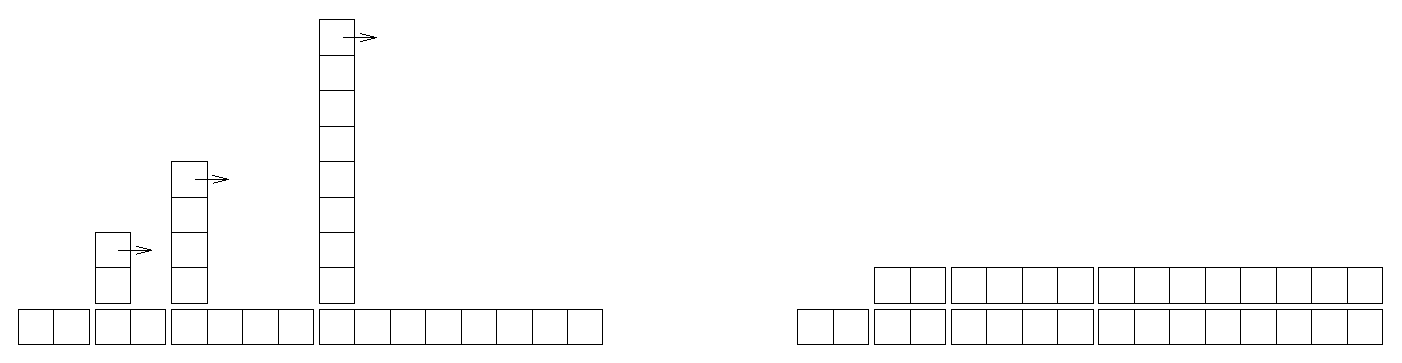
\includegraphics[scale=0.6]{figs/towers.eps}}
\caption{ハッシュ表における{\tt add}操作のコスト\label{fig.hash}}
\end{figure}

\indent　
図\ref{fig.hash}は視覚的な説明の図である。各ブロックは作業の単位時間を表す。
列は左から右へと各{\tt add}で必要とする作業時間を表現している。
「再ハッシュ」で要する作業時間は縦のタワーの系列として表現されている。
このタワーを倒して基本的な{\tt add}に要する時間ブロックに重ねてみると$n$個のアイテムを
追加するときに必要な作業時間は$2n-2$単位であることが視覚的にも分かる。\par
このアルゴリズムの重要な特徴はハッシュ表のサイズを大きくして行くときに、
幾何級数的に増やしていることだ。もしサイズを算術的に増加させる、
つまり毎回一定の固定した数だけ増やすと操作{\tt add}一つ当たりの平均時間は線形となる。\par
ハッシュマップの実装は\url{https://thinkpython.com/code/Map.py}からダウンロードできる。
しかし、Pythonではそれを使う必要はない。単に辞書を使えば済むからだ。
%
\section{語句}

\begin{description}

\item[アルゴリズムの解析（analysis of algorithms）：] 複数のアルゴリズムを実行時間と必要な記憶域
で比較する方法。
%\index{analysis of algorithms}

\item[マシンモデル（machine model）：] アルゴリズムを記述するために用いられるコンピュータの
簡単化された表現。
%\index{machine model}

\item[最悪の状況（worst case）：] そのアルゴリズムにとって実行が最遅（または記憶域を最大）になるような
入力データ。.
%\index{worst case}

\item[支配項（leading term）：] 多項式で最大の指数を持つ項。
%\index{leading term}

\item[切り換え点（crossover point）：] 二つのアルゴリズムで実行速度や必要とする記憶域が拮抗する問題のサイズ。
%\index{crossover point}

\item[増加の次数（order of growth）：] アルゴリズムの解析のために増加が同等とみなされる関数の集合。
例えば増加が線形である全ての関数は細部を無視して同じ増加の次数を持つという。
%\index{order of growth}

\item[ビック-O記法（Big-Oh notation）：] 増加の次数を表現する記法。例えば、 $O(n)$
は線形に増加する関数の照合を表現する。
%\index{Big-Oh notation}

\item[線形（linear）：] 問題のサイズが大きなところで見ると、
実行時間が問題のサイズに比例するようなアルゴリズム。
%\index{linear}

\item[方形（quadratic）：] 問題のサイズの指標$n$に対して、実行時間が$n^2$に
比例するようなアルゴリズム。
%\index{quadratic}

\item[探索（search）：] 集合（例えばリストや辞書）の中の特定の
要素の場所を特定（または存在しないこと示す）する問題。
%\index{search}

\item[ハッショ表（hashtable）：] キーと値のペアの集合であって要素の探索が集合の大きさの
よらず一定j時間でなされるような特性を持つデータ構造。
%\index{hashtable}

\end{description}
%
%
\chapter{日本語の処理（Python2版）}
ここではPythonで日本語の文字を扱うときのポイントを述べる。\par
日本語の文字をコンピュータで扱うときの問題点は第一にどのような文字が扱えるとよいかということがある。
ひらがな、カタカナは文字数が少ないからよいが漢字は文字数が多いから漢字を完璧に扱えるようにするには大変である。
「超漢字」システム（{\verb"http://ja.wikipedia.org/wiki/超漢字"}）は十七万漢字を取り扱うことができるが、これは例外的である。
よく使われる漢字に対して{\bf JIS第一水準漢字}、{\bf JIS第二水準漢字}として規格化されている約一万個の漢字がある
（{\verb"https://ja.wikipedia.org/wiki/JIS漢字コード"}）。後発ではあるがこれとは別の体系として{\bf ユニコード（Unicode）}がある。
東アジア圏の言語を纏めたCKJ統合漢字の中で扱える漢字が約二万個ある（{\verb"http://ja.wikipedia.org/wiki/Unicode"}を参照せよ）。
ユニコードで扱える漢字はJIS第一水準漢字、JIS第二水準漢字を完全に含んでいる。\par
一方漢字をどのように符号化するかも複雑である。歴史的な経緯からJISの水準漢字に対しては、
シフト{\tt JIS}、{\tt JIS}、{\tt EUC-JP}の三つ{\bf エンコード方式（符号化方式）}が使われている。
ユニコードに対しては{\tt UTF-8} のエンコード方式がよく使われる。\par
Pythonではこの四つのエンコード方式をサポートしている。これらのエンコード方式は全て8ビットの数値を一文字として扱う。
漢字一文字も複数バイトに分解して扱うので8ビット文字列と呼ぶ。
%
\section{ユニコード文字列の生成}
　これに対してユニコード文字列は英数字、ひらがな、カタカナ、漢字の一文字を平等に一文字として扱うことができる。
Pythonはこのユニコード文字列で文字列処理を行う機能を持っている。\par
ユニコード文字列を生成する方法の一つが8ビット文字列の前に「{\tt u}」をつける方方式である：
\begin{verbatim}
a = 'あいう'
au = u'あいう'
print len(a), len(au)
\end{verbatim}
この{\tt print}文で文字数を表示すると9 3とでる。
つまり、ユニコード文字列ではひらがな文字（カタカナ、漢字も）も文字数が正確に計測される。
このようにユニコード文字列で日本語を扱うと英数字の文字列に使えた関数やメソッドがそのまま日本語にも適用できる。\par
さて、インタラクティブ・モードであれスクリプト・モードであれそこに現れた日本語は何らかエンコード方式を使ってコード化されたものである。
このエンコード方式を確かめる簡単な方法がある：
\begin{verbatim}
a = 'あいう'
au = unicode(a, 'utf-8')
\end{verbatim}
これはaに代入された文字列が{\tt utf-8}でエンコードされたものみなし、ユニコードに変換を試みる関数{\tt unicode}を使った例である。
第二の引数に間違ったエンコード方式を指定するとエラーとなる。例を示す：
\begin{verbatim}
>>> a = 'あ'
>>> unicode(a,'utf-8')

Traceback (most recent call last):
  File '<pyshell#1>', line 1, in <module>
    unicode(a,'utf-8')
UnicodeDecodeError: 'utf8' codec can't decode byte 0x82 \ 
       in position 0: unexpected code byte
\end{verbatim}
このエラーが吐き出されないエンコード方式がこの日本語をエンコードしているものだとわかる。
%
\section{エンコード方式の指定}
スクリプト・モードではファイルの先頭もしくは二行目にそのファイルの日本語のエンコード方式を明示的に指定できる：
\begin{verbatim}
#coding: sjis
\end{verbatim}
このようにエンコード名（今の場合はシフト{\tt JIS}）を指定するとこのファイル内の日本語は
この指定したエンコード方式でエンコードされることになる。
このエンコード方式を明示することで簡単にユニコード文字列が生成できる。つまり、前に紹介したように文字列の前に「{\tt u}」を付ける：
\begin{verbatim}
u'あいう'
\end{verbatim}
である（インタラクティブ・モードではこの指定はできないので「{\tt u}」を付ける方法では期待したものにならない場合があるので注意）。\par
Pythonで使えるエンコード名は以下の表のようになる： \\

\begin{tabular}{|c|c|} \hline
 エンコード名の名称	&  Pythonで使うエンコード名 \\ \hline
 シフト{\tt JIS}  &  {\tt sjis}, {\tt shift-jis}, {\tt shift\_jis} \\ \hline
 {\tt JIS}  &  {\tt iso-2022-jp}  \\ \hline
 {\tt EUC-JP}  &  {\tt euc-jp}  \\ \hline
 {\tt UTF-8}  &  {\tt utf-8}  \\ \hline
\end{tabular} \\
%
\bigskip

\indent
ユニコード文字列の生成の第二の方法は{\tt unicode}関数を使うものだ：
\begin{verbatim}
a = 'あいう'
au = unicode(a, 'sjis')
\end{verbatim}
関数の第二の引数はエンコード名で明示したエンコード名を入れる。\par
第三の方法は文字列メソッドを使う方法である。
\begin{verbatim}
a = 'あいう'
au = a.decode('sjis')
\end{verbatim}
ここでもメソッドの引数には指定したエンコード名が入る。\par
さて、日本語のエンコード方式にはいくつかあることが分かったが、どのエンコード指定を使えばよいのだろうか？
スクリプト・モードでは日本語をユニコード文字列として扱うことが理想であるので、
ユニコードを一貫的に扱えるエンコード方式である{\tt UTF-8}が妥当ということになる。
%
\section{ユニコード文字列のエンコード変換}
ユニコード文字列を明示的な仕方で8ビット文字列に変換したいときには、ユニコード文字列のメソッド{\tt encode}を使う：
\begin{verbatim}
au = u'あいう'
a = au.encode('utf-8')
\end{verbatim}
これでユニコード文字列{\tt au}は{\tt utf-8}でエンコード変換され変数{\tt a}に代入される。
%
\section{辞書やタプルで日本語}
日本語を辞書やタプルで使ってみる。辞書、リスト、タプルの要素としてユニコードを使う。以下はその例である：
\begin{verbatim}
#coding: utf-8
d = { u'甲':(u'コウ', u'きのえ'),
      u'乙':(u'オツ', u'きのと'),
      u'丙':(u'ヘイ', u'ひのえ'),
      u'丁':(u'テイ', u'ひのと'),
      u'戊':(u'ボ', u'つちのえ')}
for key, value in d.items():
    print key, value
\end{verbatim}
結果の表示は以下のようになる。
\begin{verbatim}
乙 (u'\u30aa\u30c4', u'\u304d\u306e\u3068')
丙 (u'\u30d8\u30a4', u'\u3072\u306e\u3048')
丁 (u'\u30c6\u30a4', u'\u3072\u306e\u3068')
甲 (u'\u30b3\u30a6', u'\u304d\u306e\u3048')
戊 (u'\u30dc', u'\u3064\u3061\u306e\u3048')
\end{verbatim}
ユニコード文字列が辞書のキーに使えることが分かる。
この例では辞書の値はユニコード文字列のタプルになっている。
この値のタプル表示はユニコードのコードポインタに対する数字である（この状況はユニコード文字列を辞書などのデータ構造の要素とする場合に起こる）。
これを対応する文字列として表示するためにはタプルの要素を直接表示するとよい。つまり
\begin{verbatim}
for key, (v1,v2) in d.items():
    print key, v1, v2
\end{verbatim}
結果は以下のようになる：
\begin{verbatim}
乙 オツ きのと
丙 ヘイ ひのえ
丁 テイ ひのと
甲 コウ きのえ
戊 ボ つちのえ
\end{verbatim}
%
\section{日本語を含むファイル}
簡単な日本語を含むテキストファイルを作成する。
ファイル名は{\tt abc.txt}で文字コードは{\tt sjis}とする。このファイルをPythonで作成する。以下はそのプログラムである：
\begin{verbatim}
#coding: utf-8
fout = open('abc.txt','w')
uword = u'あいうえお'
fout.write(uword.encode('sjis'))
fout.close()
\end{verbatim}
ユニコード文字列を{\tt sjis}でエンコード変換してファイルに書き込んだ。 \par
今度はこのファイルを読み込んでみよう。プログラムは以下である：
\begin{verbatim}
#coding: utf-8
fin = open('abc.txt','r')
for line in fin:
    word = line.strip()
    print word, len(word)
    uword = unicode(word, 'sjis')
    print uword, len(uword)
fin.close()
\end{verbatim}
{\tt word}は8ビット文字列（{\tt sjis}）で、{\tt uword}はユニコード文字列である。結果の表示は以下のようになる：
\begin{verbatim}
あいうえお 10
あいうえお 5
\end{verbatim}
文字列の長さを{\tt len}で調べてとユニコード文字列は日本語の長さを適切に処理していることが分かる。\par
データベースに使ってみる
第14章で扱ったデータベースにユニコード文字列を使ってみる。
\begin{verbatim}
#coding: utf-8
import anydbm
import pickle
d = {u'子':u'ね', u'丑':u'うし',u'寅':u'とら',
     u'卯':u'う', u'辰':u'たつ'}
     
db = anydbm.open('abc.db','c')
for key, value in d.items():
    print key, value
    skey = pickle.dumps(key)
    svalue = pickle.dumps(value)
    db[skey] = svalue
db.close()
\end{verbatim}
データベースのキーや値としてユニコード文字列を直接使うことができないので、
{\tt dumps}関数でユニコード文字列を{\tt string}に変換して使う。\par
このデータベースの読み込みには、{\tt loads}関数を使い元のユニコードに戻す。一例を示す：
\begin{verbatim}
#coding: utf-8
import anydbm
import pickle
db = anydbm.open('abc.db')
for skey, svalue in db.items():
    key = pickle.loads(skey)
    value = pickle.loads(svalue)
    print key, len(key), value, len(value)
db.close()
\end{verbatim}
表示の結果は以下のようになる：
\begin{verbatim}
丑 1 うし 2
寅 1 とら 2
卯 1 う 1
子 1 ね 1
辰 1 たつ 2
\end{verbatim}
日本語文字の長さが正確に計測されているのが分かる。\\

\noindent
{\bf [参考文献]} \\
柴田　淳「みんなのPython」（ソフトバンククリエイティブ：2006年）
%
\chapter{日本語の処理（Python3版）}
コンピュータで扱える日本語文字の範囲については付録Cの冒頭を参照してほしい。\par
Python3ではユニコードの位置付けが著しく改良された。これは日本語にとっても朗報である。
Python3では引用符（{\tt '}）、二重引用符（{\tt "}）、三連二重引用符（{\t """}）
で囲まれた文字は全てユニコード文字として扱う。つまり{\tt str}型はユニコード文字から
なる：
\begin{verbatim}
>>> a='これも'
>>> print(a,type(a),len(a))
これも <class 'str'> 3
>>> b="これも"
>>> print(b,type(b),len(b))
これも <class 'str'> 3
>>> c="""これもユニコード"""
>>> print(c,type(c),len(c))
これもユニコード <class 'str'> 8
\end{verbatim}
文字列の長さが適切の処理されていることに注目。\par
8ビット文字列はこのユニコード文字列に{\tt b}をつけると得られる。
\begin{verbatim}
>>> d=b'a'
>>> print(d, type(d), len(d))
b'a' <class 'bytes'> 1
\end{verbatim}
しかしこの方法はマルチバイト文字では構文エラーとなる。
\begin{verbatim}
>>> e=b'あ'
SyntaxError: bytes can only contain ASCII literal characters.
\end{verbatim}
このばあいは{\tt encode}メソッドを使う：
\begin{verbatim}
>>> e='あ'
>>> f=e.encode('utf-8')
>>> print(f, type(f), len(f))
b'\xe3\x81\x82' <class 'bytes'> 3
\end{verbatim}
Python3で文字列を扱う上でよく引用される助言は：
\begin{quote}
ソフトウェアは内部では ユニコード文字列のみを利用し、入力データはできるだけ早期にデコードし、出力の直前でエンコードすべきです。
\end{quote}
%
\section{辞書やタプルで日本語}
日本語を辞書やタプルで使ってみる。辞書、リスト、タプルの要素としてユニコードを使う。以下はその例である：
\begin{verbatim}
#coding: utf-8
d = { '甲':('コウ', 'きのえ'),
      '乙':('オツ', 'きのと'),
      '丙':('ヘイ', 'ひのえ'),
      '丁':('テイ', 'ひのと'),
      '戊':('ボ', 'つちのえ')}
for key, value in d.items():
    print(key, value)
\end{verbatim}
結果は
\begin{verbatim}
甲 ('コウ', 'きのえ')
乙 ('オツ', 'きのと')
丙 ('ヘイ', 'ひのえ')
丁 ('テイ', 'ひのと')
戊 ('ボ', 'つちのえ')
\end{verbatim}
となる。辞書、タプルでも日本語が問題なく使えることがわかる（Python2ではユニコード文字列が
コードポインタに対する数字になる難点があった）。
%
\section{日本語を含むファイル}
簡単な日本語を含むテキストファイルを作成する：
\begin{verbatim}
#coding: utf-8
fout = open('abc.txt','w',encoding='utf-8')
word = '五月雨坊主'
fout.write(word)
fout.close()
\end{verbatim}
ファイル名は{\tt abc.txt}でユニコード文字列はパラメータ{\tt encoding}で指定されたエンコード方式
で8ビット文字列として保存される。今のばあいは{\tt utf-8} 。\par
このファイルを読み込むには：
\begin{verbatim}
#coding: utf-8
fin = open('abc.txt','r',encoding='utf-8')
for line in fin:
    word = line.strip()
    print(word, len(word))
    print(type(word))
fin.close()
\end{verbatim}
読み込むばあいもエンコード方式を指定する（どのような方式でエンコードされたデータであるかを
指定）。これが誤っていると読み込まれた文字列は文字化けしたものになってしまう。\par
今のばあいの結果の表示は以下のようになる：
\begin{verbatim}
五月雨坊主 5
<class 'str'>
\end{verbatim}
適切なユニコード文字列になっていることがわかる。\par
データベースに使ってみる
第14章で扱ったデータベースにユニコード文字列を使ってみる。
例として：
\begin{verbatim}
#coding: utf-8
import dbm
d = {'子':'ね', '丑':'うし','寅':'とら',
     '卯':'う', '辰':'たつ'}

db = dbm.open('abc2.db','c')
for key, value in d.items():
    print(key, value)
    db[key] = value
db.close()
\end{verbatim}
ここではユニコード文字列でできた辞書をデータベース{\tt abc2.bd}
に書き込んだ。Python3ではデータベースにユニコードを書く込む際
には文字列は自動的にエンコードされて保存される。エンコード
は{\tt utf-8}が既定値である。\par
読み込みはそのままでは8ビット文字列であるので{\tt decode}
メソッドを使ってデコードしてユニコード文字列とする：
\begin{verbatim}
#coding: utf-8
import dbm
db = dbm.open('abc2.db')
for bkey, bvalue in db.items():
    key = bkey.decode('utf-8')
    value = bvalue.decode('utf-8')
    print(key, len(key), value, len(value))
db.close()
\end{verbatim}
{\tt print}文の出力を見ると：
\begin{verbatim}
子 1 ね 1
丑 1 うし 2
寅 1 とら 2
卯 1 う 1
辰 1 たつ 2
\end{verbatim}
とユニコードとして適切に処理されていることがわかる。
%
\section{クラスで使う}
クラス定義で再定義された{\verb"__str__"}メソッドでユニコード文字列
を扱ってみる。例として：
\begin{verbatim}
coding: utf-8
class Garden(object):
    def __init__(self, plants):
        self.plants = plants
        
    def __str__(self):
        t = [ object.__str__(self) + '咲いている草花は' ]
        for obj in self.plants:
            s = '    ' + object.__str__(obj)
            t.append(s)
        return '\n'.join(t)

mygarden=Garden(['なずな','はこべら','ほどけのざ'])
print(mygarden)
\end{verbatim}
このクラス定義の{\verb"__str__"}はこの{\tt Garden}クラスのインスタンス
オブジェクトの{\tt print}に使う。この例では{\tt mygarden}がインスタンス
で{\tt print(mygarden)}がそれである。
結果の表示：
\begin{verbatim}
<__main__.Garden object at 0x0000000002F32400>咲いている草花は
    'なずな'
    'はこべら'
    'ほどけのざ'
\end{verbatim}
この例でもユニコード文字列が適切に処理されている（Python2
ではユニコード文字列に対する{\tt print}文がコードポイントの数になる難点があった）。\\

\noindent
{\bf [参考文献]} \\
\url{https://docs.python.jp/3/howto/unicode.html}
%
%
\clearpage
\phantomsection
 \addcontentsline{toc}{chapter}{訳者あとがき}
 \chapter*{訳者あとがき\markboth{訳者あとがき}{}}
 \markboth{訳者あとがき}{}
Allen Downey著``Think Python: How to Think Like a Computer Scientist(2nd Edition)"の日本語訳である。
訳者も大学の情報科学系の学生に初級プログラミングの担当をしたことがある。
{\tt C}言語を取りあげたがいくつかの問題点を感じていた。それらは、
\begin{enumerate}
\item {\tt C}言語の教育にも拘わらずポインタは難易度が高いとして省略せざるをえない。D.Knuthによればポインタは{\tt C}言語の宝庫である。
\item オブジェクト指向プログラミングについては別の言語で学習する必要がある。
\item 日本語は継子扱いである。
\end{enumerate}
Pythonはこれらの問題点のほとんどを解決してくれると訳者には思えた。\par
Pythonの大きな難点は日本語で読めるよい教科書がないことである。そのようなときに出会ったのがこのThink Pythonである。
原著者の「はじめに」にもあるように、この本は大学のプログラミングの教科書として書かれたものでる。
教科書として特徴的なことはプログラムを作成する上で不可欠のデバッグについて多くのページを割いていることである。
この点が原書を翻訳してみようとした大きな動機でもある。
原著の第二版では第一版と比べより基礎的なところから丁寧に叙述がなされおり、より教科書として
整備されてきていると感じた。\par
日本語の取り扱いについては原著では一切触れていない。Python3になってユニコードの位置づけが大幅
に変更になったので訳書では付録Cと付録DとしPython2とPython3による日本語の処理を纏めておいた。\par
この訳書が如何にプログラミングをするかといったことに感心がある読者にとって助けになれば幸である。\\

\noindent
相川利樹 \\
仙台





















\end{document}